% Copyright (c) 2002-2015 Tampere University of Technology.
%
% This file is part of TTA-Based Co-design Environment (TCE).
% 
% Permission is hereby granted, free of charge, to any person obtaining a copy
% of this software and associated documentation files (the "Software"), to
% deal in the Software without restriction, including without limitation the
% rights to use, copy, modify, merge, publish, distribute, sublicense, and/or
% sell copies of the Software, and to permit persons to whom the Software is
% furnished to do so, subject to the following conditions:
% 
% The above copyright notice and this permission notice shall be included in
% all copies or substantial portions of the Software.
% 
% THE SOFTWARE IS PROVIDED "AS IS", WITHOUT WARRANTY OF ANY KIND, EXPRESS OR
% IMPLIED, INCLUDING BUT NOT LIMITED TO THE WARRANTIES OF MERCHANTABILITY,
% FITNESS FOR A PARTICULAR PURPOSE AND NONINFRINGEMENT. IN NO EVENT SHALL THE
% AUTHORS OR COPYRIGHT HOLDERS BE LIABLE FOR ANY CLAIM, DAMAGES OR OTHER
% LIABILITY, WHETHER IN AN ACTION OF CONTRACT, TORT OR OTHERWISE, ARISING
% FROM, OUT OF OR IN CONNECTION WITH THE SOFTWARE OR THE USE OR OTHER DEALINGS
% IN THE SOFTWARE.
\documentclass[twoside]{tceusermanual}
\usepackage{pslatex,verbatim}

% for index
\makeindex

\begin{document}
\title{TTA-based Co-design Environment v1.13}
\ver{31}
\firstday{2006-10-25}
\lastday{2016-02-18}
% id number in P- sequence
\docnum{1000}
% draft/complete/committedt
\state{complete}
\maketitle

% Table of contents
\tableofcontents

% Document text
\chapter{INTRODUCTION}

%\section{Document Overview}
This is the user manual for TTA Co-design Environment (TCE)
\cite{tcewww}
\cite{lptce1}
%\cite{lptce}. 
The document describes all the tools in the toolset, and a set of common use 
cases in the form of tutorials.

Fig.\ref{fig:tce_overview} shows a simplified overview of TCE. TCE supports
programs written in C/C++ and OpenCL. User can easily design new customized
Transport-Triggered Architecture (TTA) processors, compile the program,
analyze the performance, and generate HDL implementations of the designed
processors. The generated application-specific processor HDL can be 
synthesized for example to an FPGA chip. Then, user can modify the 
application and upload new program image to continue development.

\begin{figure}
  \begin{center}
    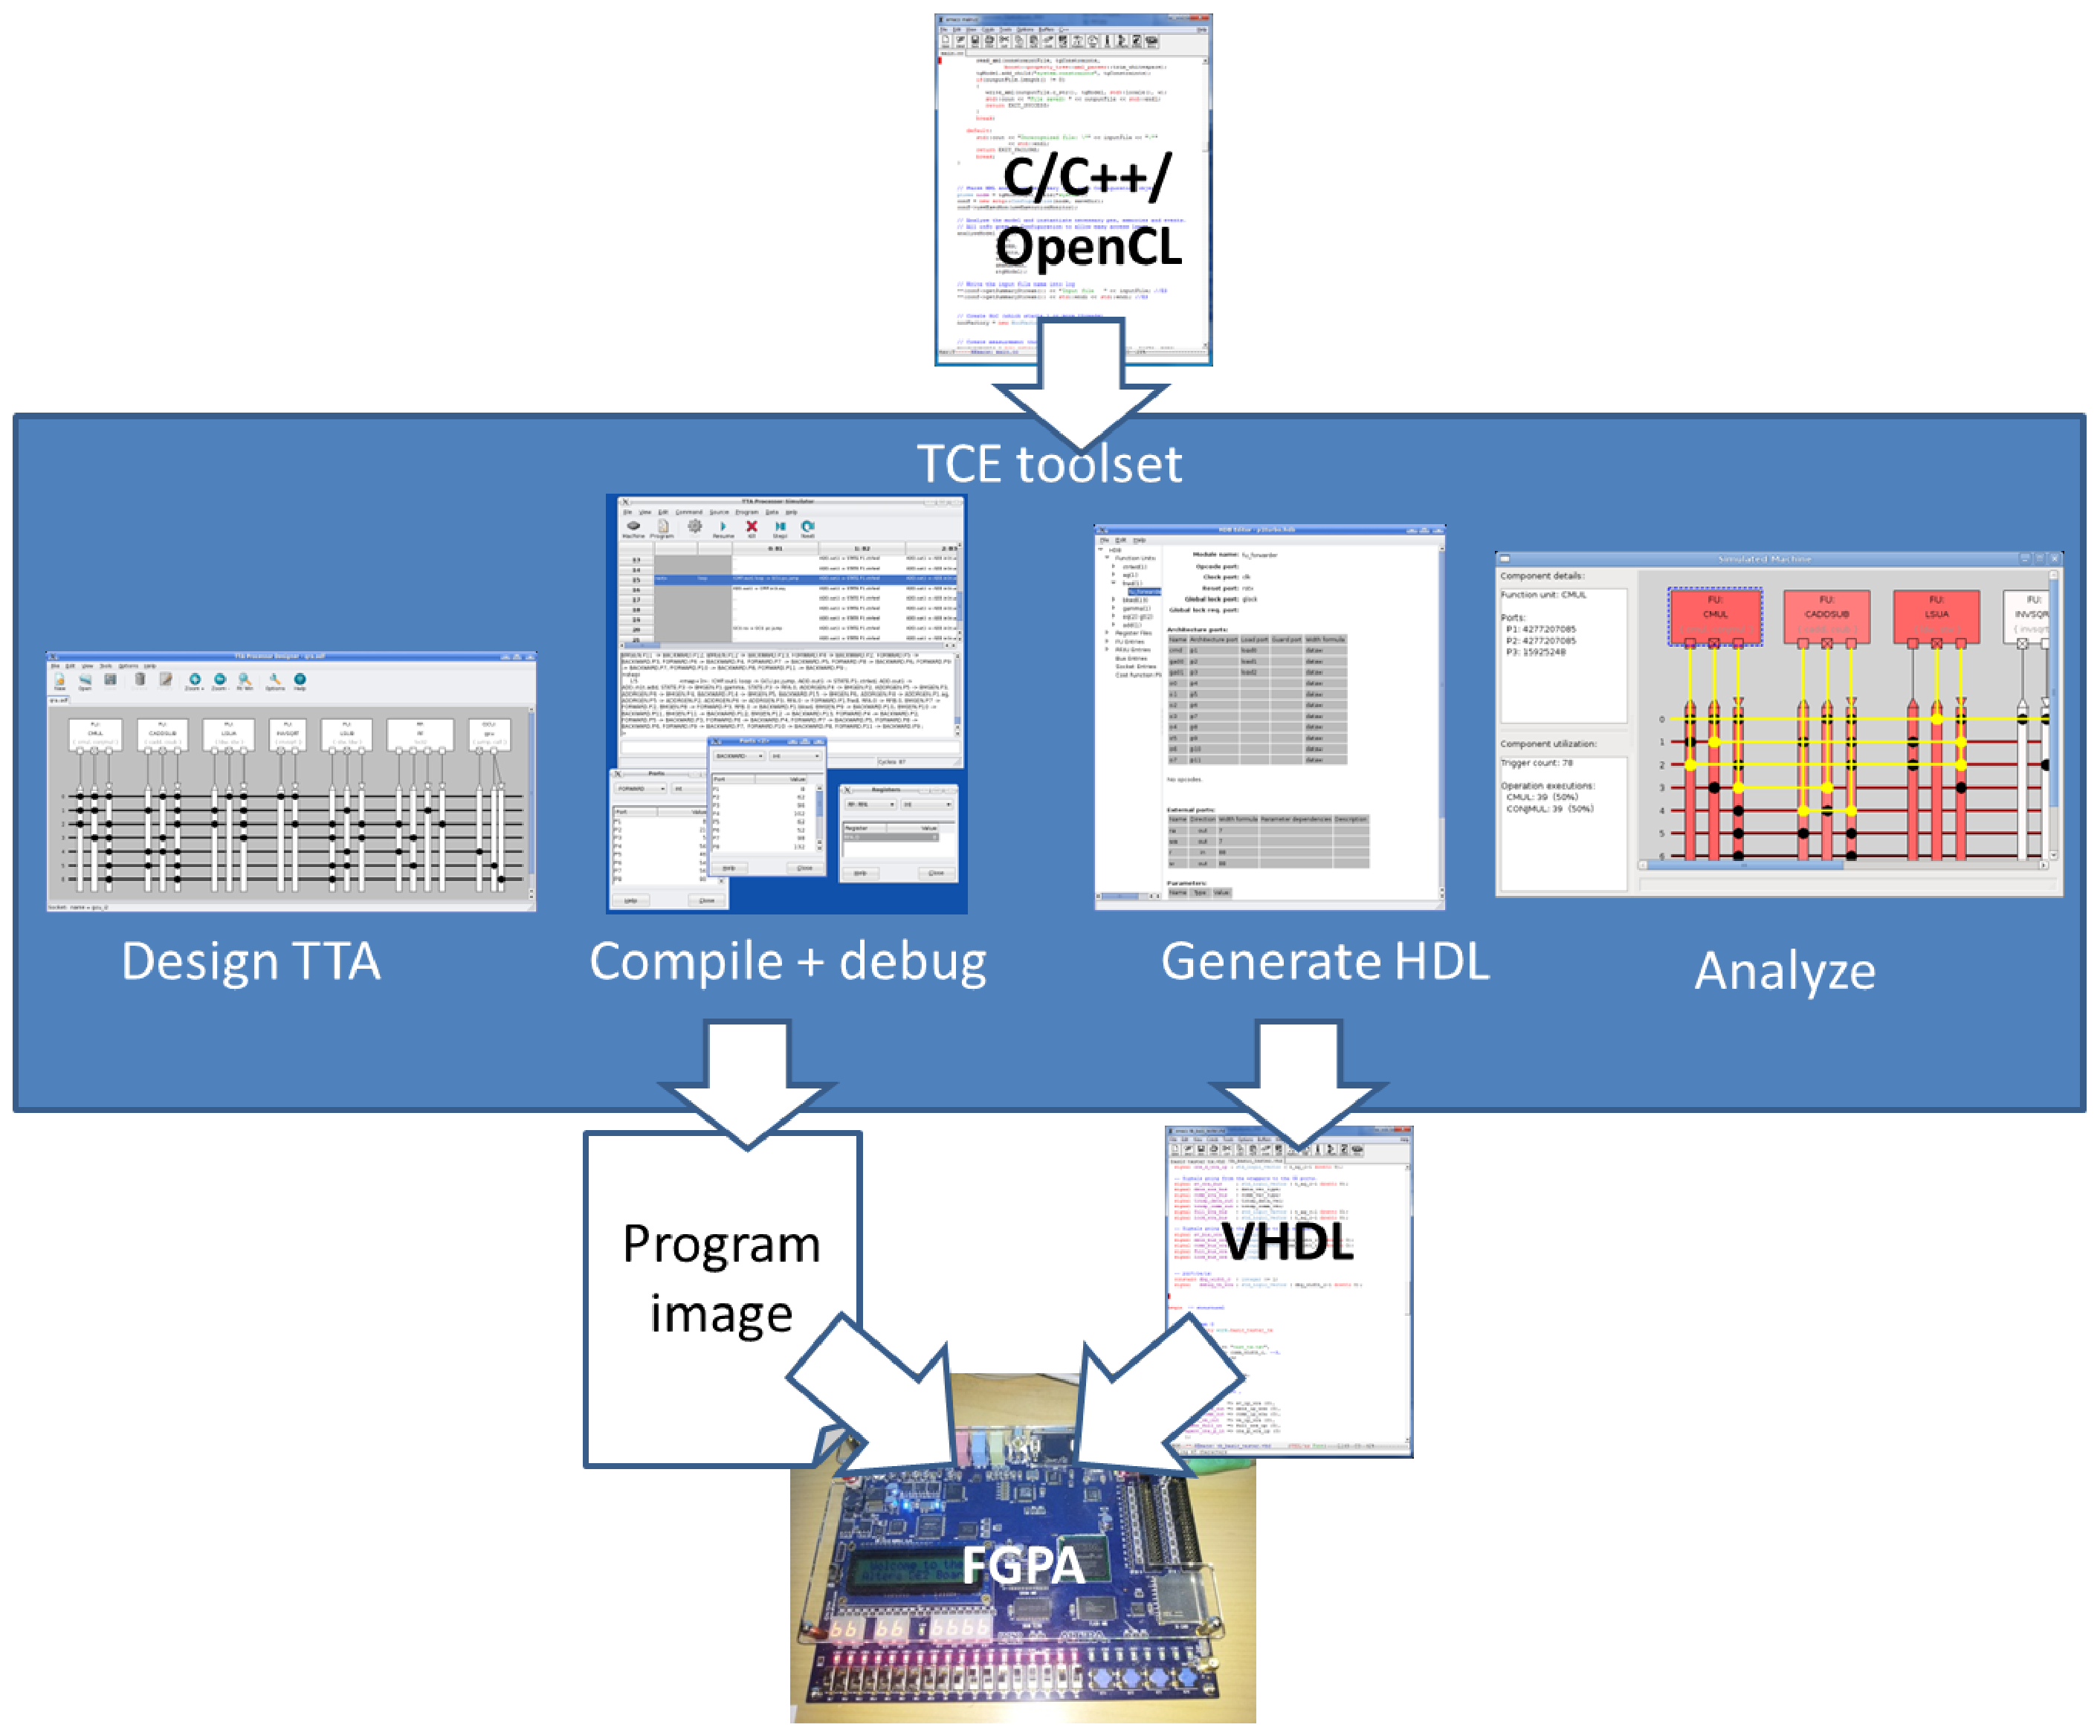
\includegraphics[width=10cm]{eps/tce_overview}
    \caption{Overview of TTA Co-design Environment (TCE).}
    \label{fig:tce_overview}
  \end{center}
\end{figure}

Application-specific instruction-set processor (ASIP) is a
programmable processor which is tailored to certain application
(domain). Hence, it can outperform general-purpose processors in terms
of performance, area, and power. On the other hand, the programmability
and the powerful ASIP tools should provide increased productivity in
comparison to fixed function accelerator implementations, which offer the
highest performance.

With TCE, TTA ASIP configuration, SW compilation, and simulation can
be carried out in the order of minutes and hence most of the time can
be reserved to application and architecture co-development. It is fast
to iterate over new TTA configurations, e.g., change the number and
type of function units (FU), configure interconnection network (IC),
register files (RF), or experiment with special function units 
(custom operations).  

Simple TTA designs with support for a couple of
parallel arithmetic operations consume in the order of
approx. 1000-5000 LUTs (look-up tables), which means that modern FPGA's
can easily include even tens of TTA cores. The operating clock frequency can
be optimized to match the soft cores offered by FPGA vendors.

\section{Document Overview}

Chapter~\ref{chapter:tceFlow} provides an overview to the TCE
processor design flow, and Chapter~\ref{chapter:tutorials} contains
tutorials for several common TCE use cases. These should be sufficient
for starting to use the TCE toolset.  The rest of the chapters
describe the use of each tool separately, and they can be referred to
for information on more advanced usage the tools.

Many people have contributed to this document, most notably Pekka
J��skel�inen, Otto Esko, Heikki Kultala, Vladimir Guzma and Erno
Salminen.


\section{Acronyms, Abbreviations and Definitions}
\begin{tabular}[h]{p{0.15\textwidth}p{0.80\textwidth}}
ADF & (Processor/Machine) Architecture Definition File.\\
BEM & Binary Encoding Map. Describes the encoding of instructions.\\
CLI & Command Line Interface\\
ExpResDB  & Exploration Result Database.\\
GUI & Graphical User Interface \\
GPR & General Purpose Register \\
HDB & Hardware Database \\
HDL & Hardware Description Language. \\
HLL & High Level (Programming) Language. \\
IDF & (Machine/Processor) Implementation Definition File.\\
ILP & Instruction Level Parallelism.\\
LLVM & Low Level Virtual Machine \\
MAU & Minimum Addressable Unit\\
PIG & Program Image Generator\\
SQL & Structured Query Language.\\
TCE & TTA Co-design Environment.\\
TPEF & TTA Program Exchange Format \\
TraceDB & Execution Trace Database. \\
TTA & Transport Triggered Architecture.\\
VHDL & VHSIC Hardware Description Language. \\
XML & Extensible Markup Language. \\
\end{tabular}

\section{Typographic Conventions Used in the Document}

\begin{center}
\begin{tabular}{p{0.30\textwidth}|p{0.63\textwidth}}
\hline
\textbf{Style} &\textbf{Purpose}\\
\hline
\hline
\emph{italic}     & parameter names in running text\\
\hline
[brackets]        & bibliographic references\\
\hline
`single quoted'   & keywords or literal strings in running
                    text\\
\hline
\file{file name}   & file and directory names in running text\\
\hline
\textbf{bold}     & Shorthand name of a TCE application.\\
\hline
\shellcmd{courier}     & UNIX commands\\
\hline
\end{tabular}
\end{center}


\chapter{PROCESSOR DESIGN FLOW}
\label{chapter:tceFlow}


The main goal for the TTA Co-design Environment (TCE) is to provide a
reliable and effective toolset for designing programmable application
specific processors, and generate machine code for them from
applications written in high-level languages, such as C, C++ or
OpenCL.
\begin{figure}
  \begin{center} 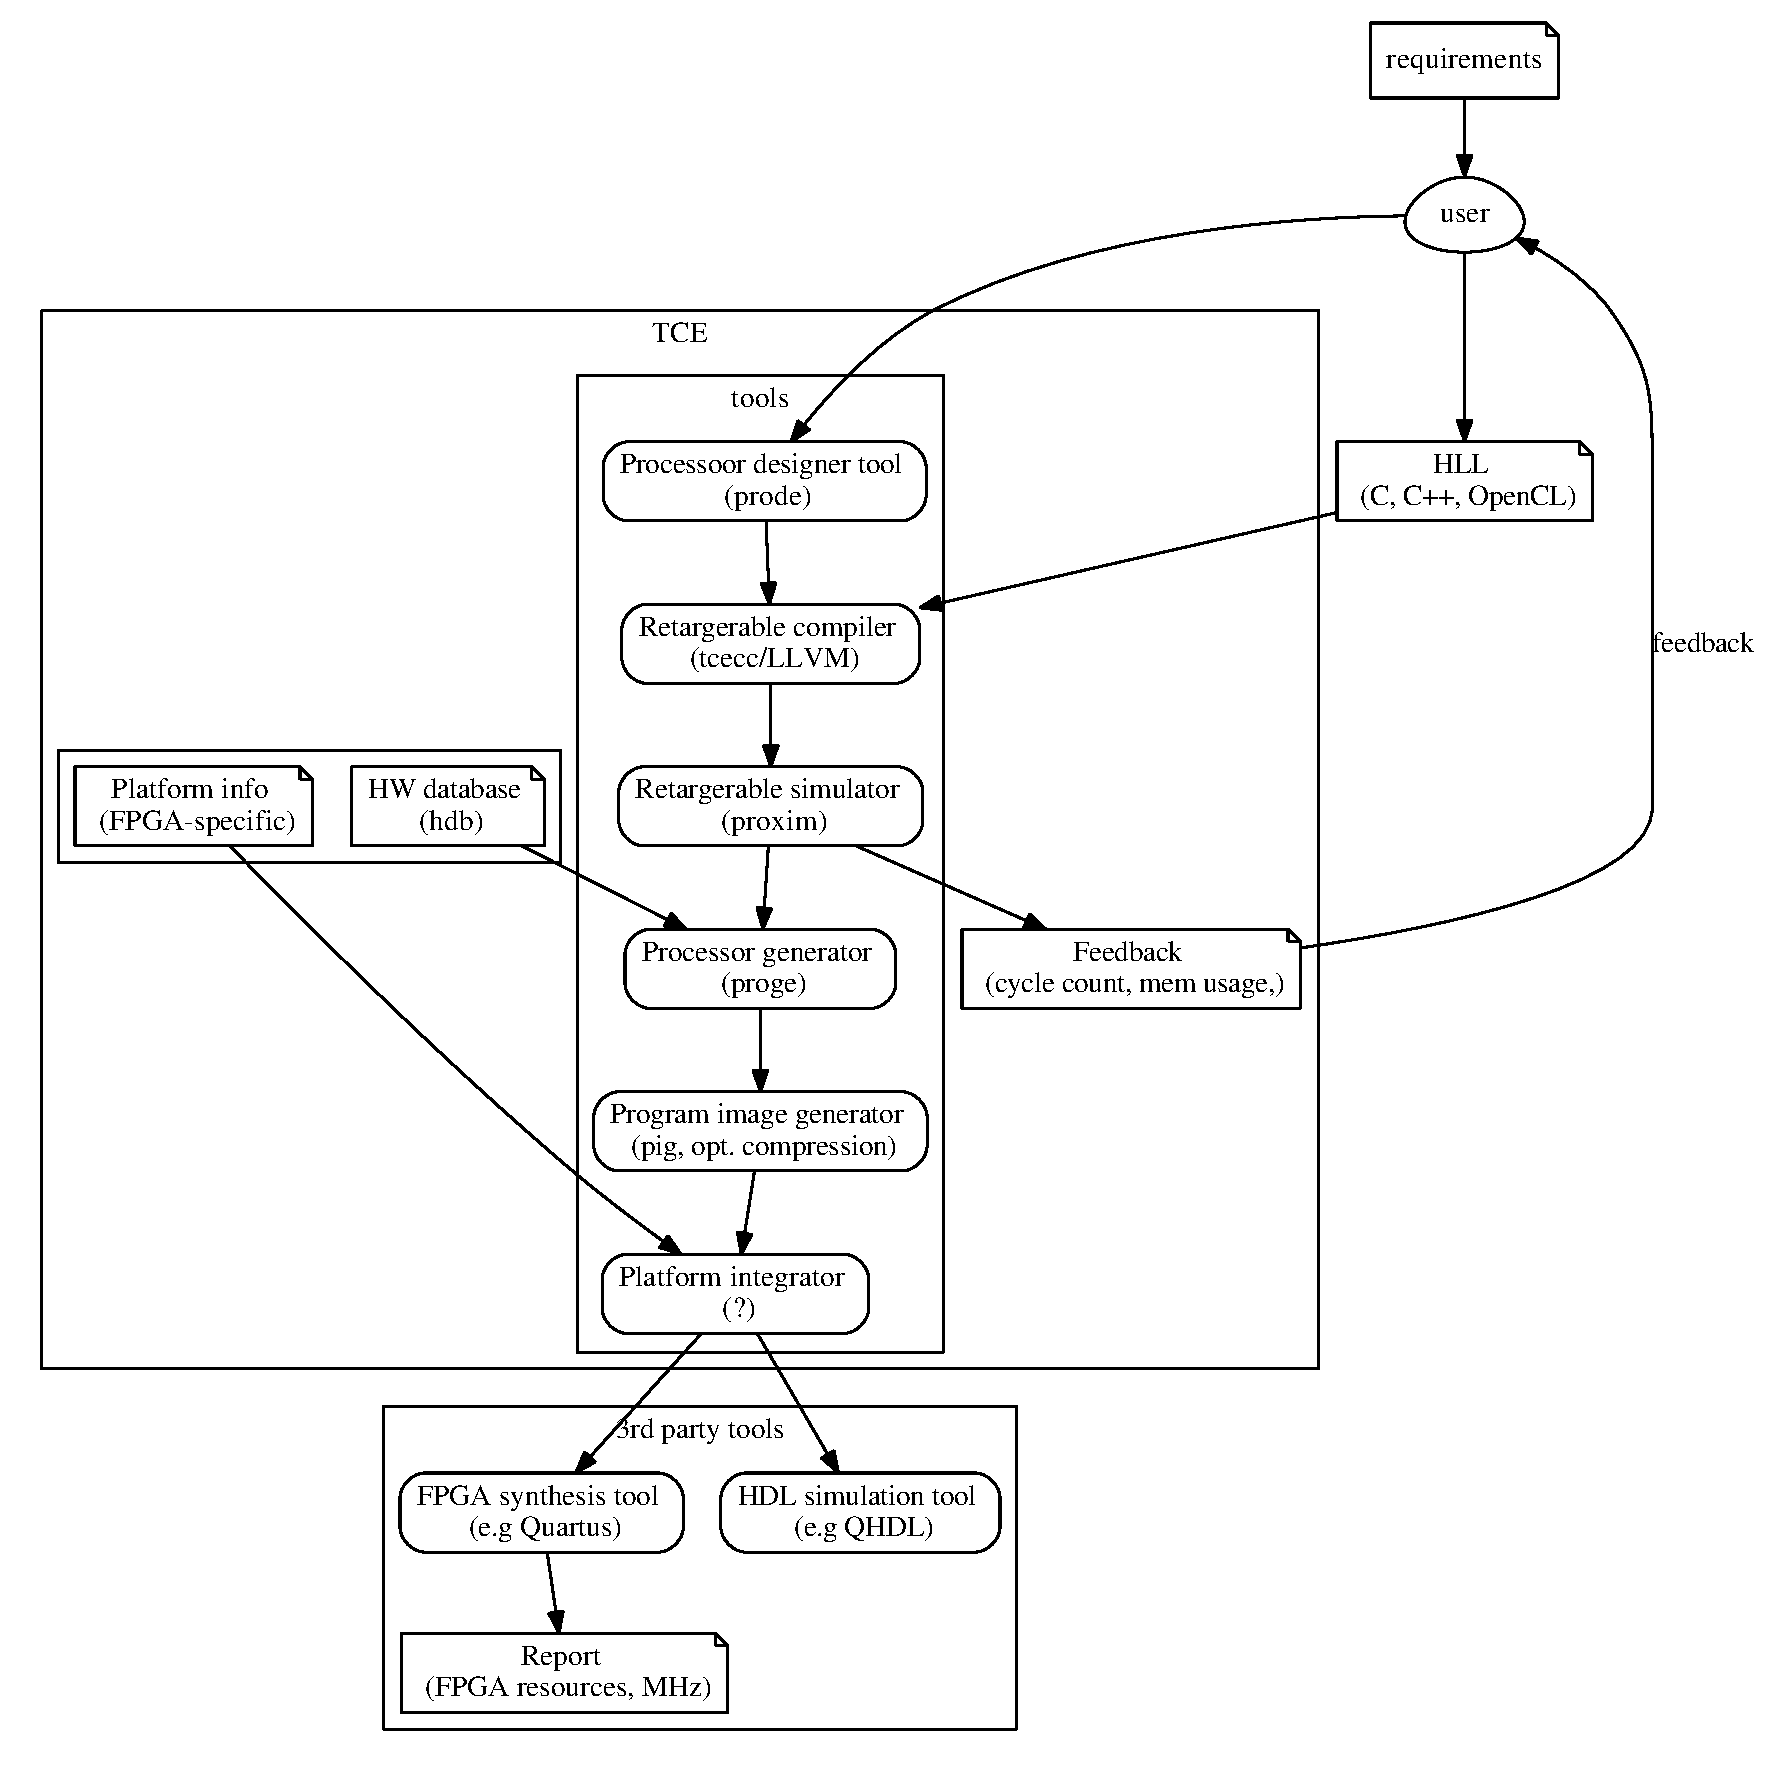
\includegraphics[width=10cm]{eps/tce_flow}
  \caption{Overview of TTA Co-design Environment (TCE). } 
  \label{fig:tce_flow} \end{center}
\end{figure}

In addition, TCE provides an extensible research platform for 
experimenting with new ideas for Transport Triggered Architectures (TTAs), 
retargetable ILP code generation, and application specific processor 
design methodology, among others.

\section{Design Flow Overview}

The main phases in the TCE are illustrated in
Figure~\ref{fig:tce_flow} and listed in Table~\ref{tab:phases} The
TCE design flow starts from an application described in a high level
language (currently the C language).  The initial software development
phase is intended to be separate from the actual co-design flow of
TCE. That is, the program is expected to be implemented and tested
natively (on a workstation PC) before ``porting'' it to the TTA/TCE
platform. The porting includes ensuring that TTA/TCE runs the program
correctly, and optimizing the hardware together with the software by
modifying the resources and architecture of the processor to fit the
application at hand -- a process called hardware/software co-design.

Once the user has implemented the software based on requirements, he
designs a TTA processor with a graphical tool, or selects an existing
TTA, and compiles and simulates the SW. Both compiler are simulator are
\textit{retargetable} so they need an architectre definition as 
input in addition to SW source codes. The instruction set simulator (Proxim
or ttasim) produces statistics about cycle counts and utilization of function 
unit, to assist in iteration of the SW of TTA HW until results are satiscatory.

The LLVM compiler framework~\cite{llvm-home-page} is used to compile
the application to 'bitcode', the intermediate representation of
LLVM. The resulting bitcode is then compiled and scheduled to a
particular TTA processor by TCE. Traditional compiler optimizations
are done in LLVM before bitcode generation, so it is possible to
utilize the same bitcode file when exploring different TTA processors
for running an application.
% ISO C99 if LLVM/TCE is used

Once the performance requirement is met, the user maps the
architectural resources i.e. function units and register files, to
their respective RTL implementations which are stored in Hardware
Databases (HDB). The distinction between architectural models and
component implementations makes it possible to have several
implementations, each e.g. targeted for different FPGA families or
ASIC technologies, stored in HDBs. Ideally, changing the target
platform might only require changes to the implementation mapping
without any changes to the architecture.

After the implementation mapping, the Processor Generator (ProGe) can
produce synthesizable HDL, which instantiates all FUS and creates the
interconnection network and control unit, which is responsible of
fetching, decoding and issuing instructions. ProGe tool also includes
a platform integrator feature which can interface the TTA with memory
components of an FPGA board and create synthesis settings. Moreover,
the platform integrator can ``package'' the TTA (and optionally also the
SW) into an easily re-usable format. In practice, this means generating
IP-XACT documents which describe the details in XML. Synthesing and
simulating the HDL are done with 3rd party tools, such as Altera's
Quartus and Mentor Graphics' Modelsim.

Finally, Program Image Generator (PIG) is utilized to convert the 
compiled SW format into actual binaries. PIG supports various
different output formats ranging from plain binary format to FPGA
vendor specific embedded RAM formats.

More details about the tools and design phases are given in Chapters
\ref{sec:prode} - \ref{section:codesign}. The TCE tour tutorial in
section~\ref{sec:tcetour} provides a hands-on introduction to the design
flow.

\begin{table}
  \begin{center}
    \caption {Summary of tools. Some of the tools have grahical
    user interface (GUI) and others executed from the shell command
    line (CLI).}
    \label {tab:phases}
    \begin{tabular}{l | l | l | l }
      \hline
      Tool & Purpose & Type & Output file(s)\\
      \hline
      \hline
      ProDe                & Define FUs, registers, intercconects of TTA core & GUI  & .adf \\
      tcecc                & Compile software                                 & CLI  & .tpef \\
      Proxim               & Simulate TTA cores (architectural level)         & GUI  & report \\
      ttasim               & Simulate TTA cores (architectural level)         & CLI  & report \\
      OSEd                 & Operation Set Abstraction Layer database editor  & GUI  & operation db \\
      HDBEditor            & HW implementation database editor                & GUI  & HDB  \\
      \hline
      ProGe / generateprocessor             & Generate HDL                    & CLI (+GUI) & VHDL or Verilog \\
      PIG / generatebits   & Generate program image                           & CLI  & e.g. .mif  \\
      Platform integrator  & Interface with memories, generate IP-XACT        & CLI  & e.g. .xml, project files \\
      \hline
      3rd party Synthesis  & Convert VHDL to netlist and program FPGA         & G/C  &  e.g. .sof\\
      3rd party Simulation & Simulate VHDL                                    & G/C  &  report, .wave \\
      \hline
    \end{tabular}
  \end{center}
\end{table}


\section{Main File Formats}
\label{section:fileFormats}

The flow consists of many separate tools and information is exchanged
with files.  This chapter gives an overview of 8 file and database
types manipulated by TCE applications and accessible to users of the
toolset, architecture definition .adf and SW binary
.tpef being the most important ones. Many files are XML so
user can easily access them, if needed.

There a 3 kind of files:

\begin{enumerate}
 \item HW definitions: adf, hdb, and idf
 \item SW definitions: tpef, bem, opp, cc, opb
 \item Simulation and exploration data: dsdb, set of the files above
\end{enumerate}

%%% !!! INSERT BASIC EXPLANATION !!!

%\begin{figure}
%  \centerline{\psfig{figure=eps/design_flow_selection.eps,width=0.35\textwidth
%  }}
%  \caption{Processor Configuration Selection.}
%  \label{fig:design_flow_selection}
%\end{figure}

%\begin{figure}
%  \centerline{\psfig{figure=eps/design_flow_codegen.eps,width=0.6\textwidth}}
%  \caption{Code Generation and Analysis.}
%  \label{fig:design_flow_codegen}
%\end{figure}

%\begin{figure}
%  \centerline{\psfig{figure=eps/design_flow_generation.eps,
%      width=0.85\textwidth}}
%  \caption{Processor and Program Image Generation.}
%  \label{fig:design_flow_generation}
%\end{figure}

%Figure~\ref{fig:design_flow_exploration} the design space 
%exploration phase, Figure~\ref{fig:design_flow_selection} the processor 
%configuration selection phase, Figure~\ref{fig:design_flow_codegen} the 
%code generation and analysis phase, and Figure~\ref{fig:design_flow_generation} 
%the generation of the final outputs: the processor description and the 
%program bit image.

\subsection{Architecture Definition File (ADF)}
\label{sec:adf}

Filename extension: .adf

Architecture Definition File (ADF) is a file format for
defining target processor architectures, e.g. which function units are
used and how they are connected \cite{ADF-specs}.  ADF can be created with
ProDe manually or, e.g., by automated design space exploration tools. ADF 
is a specification of the target ``processor architecture'', meaning that only 
the information needed to generate valid programs for the processor is stored, 
but nothing else. This file is needed by many tools, such as tcecc, ttasim, and ProGe.

The XML snippet below gives an idea of ADF.
\begin{verbatim}
<adf version="1.7">

  <bus name="B1">
    <width>32</width>
    <guard>
      <always-true/>
    ...
  <socket name="alu_comp_i1">
    <reads-from>
      <bus>B1</bus>
    ...
  <function-unit name="alu_comp">
    <port name="in1t">
      <connects-to>alu_comp_i1</connects-to>
      <width>32</width>
      <triggers/>
    ...
    <operation>
      <name>add</name>
      <bind name="1">in1t</bind>
      ...
  <register-file name="RF">
    <type>normal</type>
    ...
  <address-space name="data">
    <width>8</width>
    ...
\end{verbatim}

\subsection{TTA Program Exchange Format (TPEF)}
\label{section:TPEF}

Filename extension: .tpef

TTA Program Exchange Format (TPEF) is a file format for storing
compiled TTA programs which can be either unscheduled, partially
scheduled, or scheduled
\cite{TPEF-specs}. TPEF supports auxiliary sections for storing
additional information related to the program, such as execution
profiles, machine resource data, and target address space definitions.
This file is needed, e.g.  by ttasim and Pig.

\subsection{Hardware Database (HDB)}
\label{section:hdb}
% Describe what is shipped by default in TCE
Filename extension: .hdb

Hardware Database (HDB) is the main SQLite database used by the
Processor Generator and the Cost Estimator.  The data stored in HDB consist
of hardware description language definitions (HDL) of TTA components
(function units, register files, buses and sockets) and metadata that
describe certain parameters used in implementations. In addition, HDB may
include data of each implementation needed by the cost estimation
algorithms.

TCE ships with an example HDB that includes implementations for several
function units and register files in VHDL, and cost data for the default
interpolating cost estimation plugin. 

\subsection{Implementation Definition File (IDF)}
\label{sec:idf}

Filename extension:  .idf

Describes which implementations to use for each component in the
architecture. Hence, this links architectural components described in 
ADF files to implementation alternatives stored in HDB. Using this
information it is possible to fetch correct hardware description
language (HDL) files from the hardware block library for cost
estimation and processor generation. This file is needed, by
ProGe and PIG.


The XML snippet below gives an idea of IDF.
\begin{verbatim}
 <adf-implementation>
  ...
  <fu name="LSU">
    <hdb-file>asic_130nm_1.5V.hdb</hdb-file>
    <fu-id>62</fu-id>
  </fu>
  ...
\end{verbatim}



\subsection{Binary Encoding Map}
\label{sec:bem}

Filename extension: .bem 

Provides enough information to produce an executable uncompressed bit
image 
%(Section~\ref{sec:db_bim}) 
from TPEF program data.


\subsection{Operation Set Abstraction Layer (OSAL) Files}
\label{section:osal}
% Describe what is shipped by default in TCE
Filename extension: .opp, .cc, .opb

OSAL stores the simulation behavior and static properties of operations 
that can be added to the function units in the designed processors.

Simulation behavior of function unit operations is described by implementing
simulation functions which can be plugged in to the simulator run time.

The .opp file is an XML file for defining the static properties of
operations (for example, how many inputs and outputs an operation
has). The .cc is the C++ source file that defines the behavior model
for a set of operations. The .opb is the plugin module compiled from
the .cc.  OSAL is quite complex and further details are presented in
Section~\ref{section:osal_details}.


\subsection{Simulation Trace Database}
\label{sec:tracedb}

Filename extension: .tracedb

Stores data collected from simulations and used by instruction scheduler
(profiling data) and cost estimator (utilization statistics, etc.).

\subsection{Exploration Result Database}
\label{sec:expresdb}

Filename extension: .dsdb

Exploration Result Database (ExpResDB) contains the configurations that have
been evaluated during exploration (manual or automatic) and a summary of
their characteristics. Files that define each tested configuration (ADF and
IDF) are stored in the database as well. 



\subsection{Summary of file types}
\label{sec:summary}

Table~\ref{tab:files} summarizes briefly the most common TCE file types.

\begin{table}[b]
  \begin{center}
    \caption {Summary of file types}
    \label {tab:files}
    \begin{tabular}{l | l | l }
      \hline
      Postfix  & Purpose                                    & Format \\
      \hline
      \hline
      adf      & Architecture description                 & XML \\
      idf      & Implementation/microarchitecture description & XML \\
      hdb      & HW database                                & SQLite \\
      \hline
      tpef     & TTA program exchange format                & bin \\
      bem      & Binary encoding map                        & bin \\
      opp      & Operation properties                       & XML \\
      cc       & Simulation behavior of an operation                   & C++\\
      opb      & Compiled operation behavior                & bin \\
      \hline
      tracedb  & Database of simulation and cost estimation results     & SQLite \\
      dsdb     & Database of exploration results and TTA configurations & SQLite \\
      \hline
    \end{tabular}
  \end{center}
\end{table}


\chapter{TUTORIALS AND HOW-TOS}
\label{chapter:tutorials}

This section presents 11 tutorials covering the basics, printing and
streaming I/O, floating-point computation, parallel assembly, multiple
memories, FPGA considerations and programming TTAs using OpenCL C.

Let's start with the simplest one.

\section{TCE Tour}
\label{sec:tcetour}

This tutorial goes through most of the tools in TCE using a fairly simple
example application. It starts from C code and ends up with VHDL of the
processor and a bit image of the parallel program. This tutorial will also
explain how to accelerate an algorithm by customizing the instruction
set, i.e., by using custom operations. The total time to go through
the tutorial is about $2-3$ hours.

The tutorial file package is available at:

\url{http://tce.cs.tut.fi/tutorial_files/tce_tutorials.tar.gz}\\

Fetch and unpack it to a working directory and then enter the directory:

\begin{verbatim}
> wget http://tce.cs.tut.fi/tutorial_files/tce_tutorials.tar.gz
> tar -xzf tce_tutorials.tar.gz
> cd tce_tutorials/tce_tour
> ls -la

total 84
drwxr-xr-x 3 tce tce  4096 2010-05-28 11:40 .
drwx------ 7 tce tce  4096 2012-05-18 13:22 ..
-rw------- 1 tce tce  5913 2010-03-08 20:01 crc.c
-rw------- 1 tce tce  1408 2008-11-07 11:35 crc.h
-rw------- 1 tce tce  3286 2008-11-07 11:35 crcTable.dat
-rw-r--r-- 1 tce tce  2345 2010-03-08 13:04 custom_operation_behavior.cc
-rw-r--r-- 1 tce tce   855 2010-05-28 11:41 custom_operations.idf
-rw------- 1 tce tce  1504 2010-03-08 20:01 main.c
-rw-r--r-- 1 tce tce 45056 2010-03-10 16:09 tour_example.hdb
drwxr-xr-x 2 tce tce  4096 2010-05-28 11:40 tour_vhdl
\end{verbatim}


\subsection{The Sample Application}

The test application counts a 32-bit CRC (Cyclic Redundant Check)
check value for a block of data, in this case 10 bytes. The C code
implementation is written by Michael Barr and it is published under
Public Domain. The implementation consists of two different version of
crc, but we will be using the fast version only.

The program consists of two separate files: \file{main.c} contains the
simple main function and \file{crc.c} contains the actual
implementation. Open \file{crc.c} in your preferred editor and take a
look at the code. Algorithm performs modulo-2 division, a byte at a
time, reflects the input data (MSB becomes LSB) depending on the
previous remainder, and XORs the remainder with a predefined
polynomial (32-bit constant). The main difference between the crcSlow
and crcFast implementations is that crcFast exploits a precalculated
lookup table. This is a quite usual method of algorithm optimization.

% \subsection{Generating LLVM Bitcode}
% 
% We first generate LLVM bitcode from the C code. The bitcode
% will be later compiled to an architecture dependent TTA program.
% Compile the C code with the 'tcecc' compiler:
% 
% \shellcmd{tcecc -O3 -o crc.bc -k result -D\_DEBUG crc.c main.c}
% 
% This produces an architecture independent bitcode program \file{crc.bc}
% of the C code. The switch -k was used to tell the
% compiler to keep the \textit{result} symbol in the
% generated program in order to access them by name in the simulator.

\subsection{Starting Point Processor Architecture}
\label{ssec:start_point}
We use the {\em minimal architecture} as the starting point. File
\file{minimal.adf} describes a minimalistic architecture containing
just enough resources that the TCE compiler can still compile programs for it. 
Function units in \file{minimal.adf} are selected from the hardware
database (HDB, Section~\ref{section:hdb}) so we are able to generate a VHDL
implementation of the processor automatically later in the tutorial.
% It is also possible to
% design all the components from scratch in order to evaluate the architecture
% without actually implementing the components in VHDL.

Copy the \file{minimal.adf} included in TCE distribution to a new ADF
file which is your starting point architecture. You can view it using the
graphical Processor Designer (ProDe, Section~\ref{sec:prode}) tool:

\shellcmd{cp \$(tce-config -{}-prefix)/share/tce/data/mach/minimal.adf start.adf}

\shellcmd{prode start.adf \&}

Fig.~\ref{fig:prode} shows how Prode should look like. There is 1 bus
and 5 units: global control unit (GCU), 2 register files , 1 ALU ,and
1 LSU.
\begin{figure}
  \begin{center}
    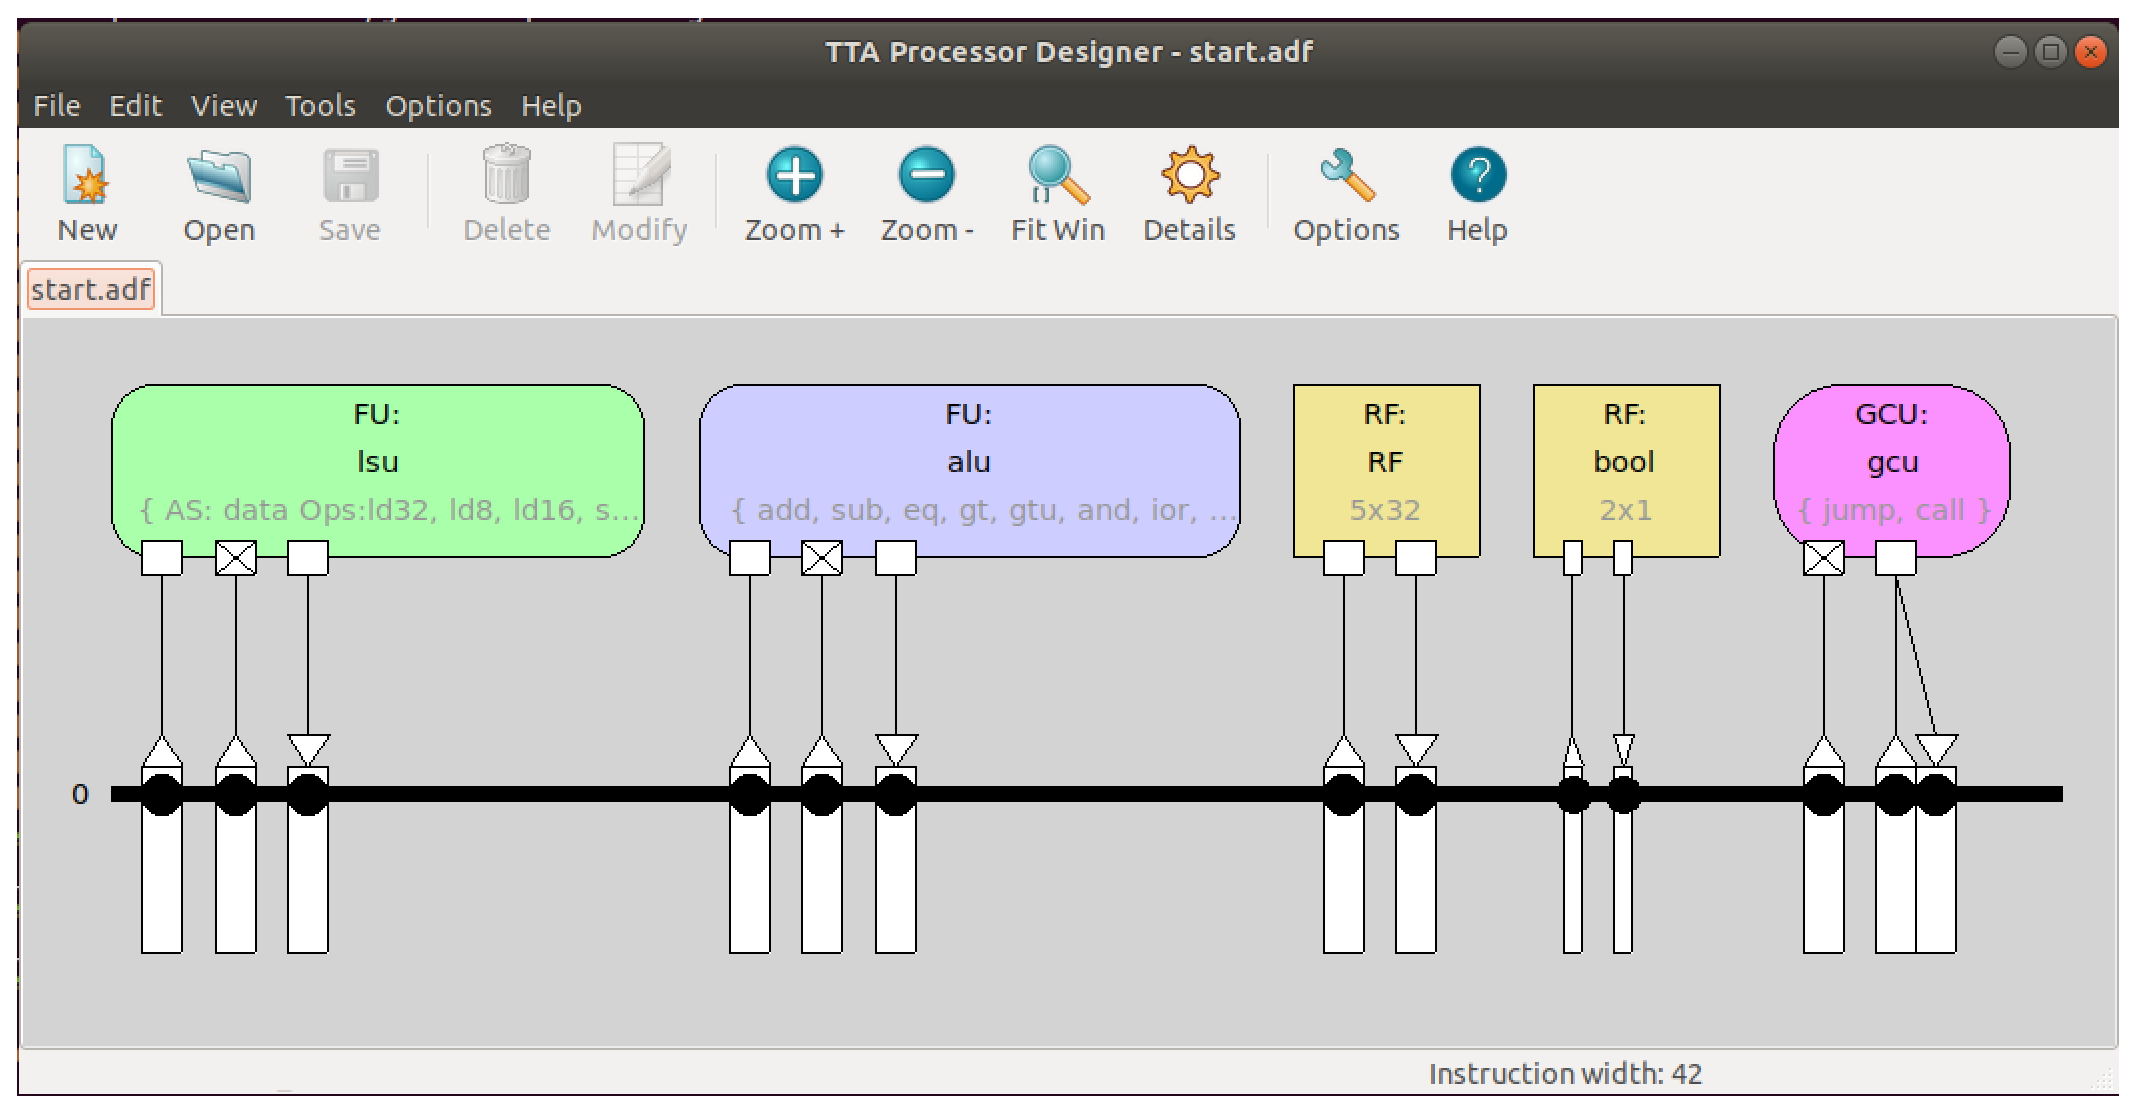
\includegraphics[width=10cm]{eps/prode_scrshot}
    \caption{Processor Designer (prode) when minimal ADF is opened}
    \label{fig:prode}
  \end{center}
\end{figure}

You'll learn how to edit the TTA with ProDe later in this tutorial.

If you want later to simulate the generated processor using GHDL
(Section \ref{ssec:tcetour_final_products}), you should decrease the
amount of memory in the processor already now. Otherwise the GHDL
executing the generated testbench might consume tremendous amount of
memory on your computer and even crash. Select
\textit{Edit -> Address Spaces} in ProDe. Then edit the bit widths of
data and instruction address spaces and set them to $15$ bits which
should be plenty for our case.


\subsection{Compiling and simulating}
\label{ssec:eval_start}
Now we want to know how well the starting point architecture executes
our program. We must compile the source code for this architecture
with command:

\shellcmd{tcecc -O3 -a start.adf -o crc.tpef -k result main.c crc.c}

In addition to source codes, the compiler needs the TTA architecture
definition \file{start.adf}. It will produce a parallel program called
\file{crc.tpef} which can only be executed on this architecture. The
switch $-k$ tells the compiler to keep the \textit{result} symbol
(variable on line 29 of main.c) also in the generated program in order
to access the variable contents by name in the simulator later on.

Successful compilation does not print anything and we can now simulate
the program. Let's use graphical user interface version of the
simulator called Proxim (Section~\ref{section:proxim}):

\shellcmd{proxim start.adf crc.tpef \&}

The simulator will load the architecture definition and the program
and wait for commands. Proxim shows one line per instruction. Minimal
TTA has only bus and hence there is only instruction slot
(column). The total number of instructions is about $1~200$.

Execute the program by clicking ``Run'' and Proxim should look like
Fig.~\ref{fig:proxim}.  Write down this cycle count in the bottom bar
of the simulator, you can use Table~\ref{tab:cyclecounts}. for future comparison.
\begin{figure}
  \begin{center}
    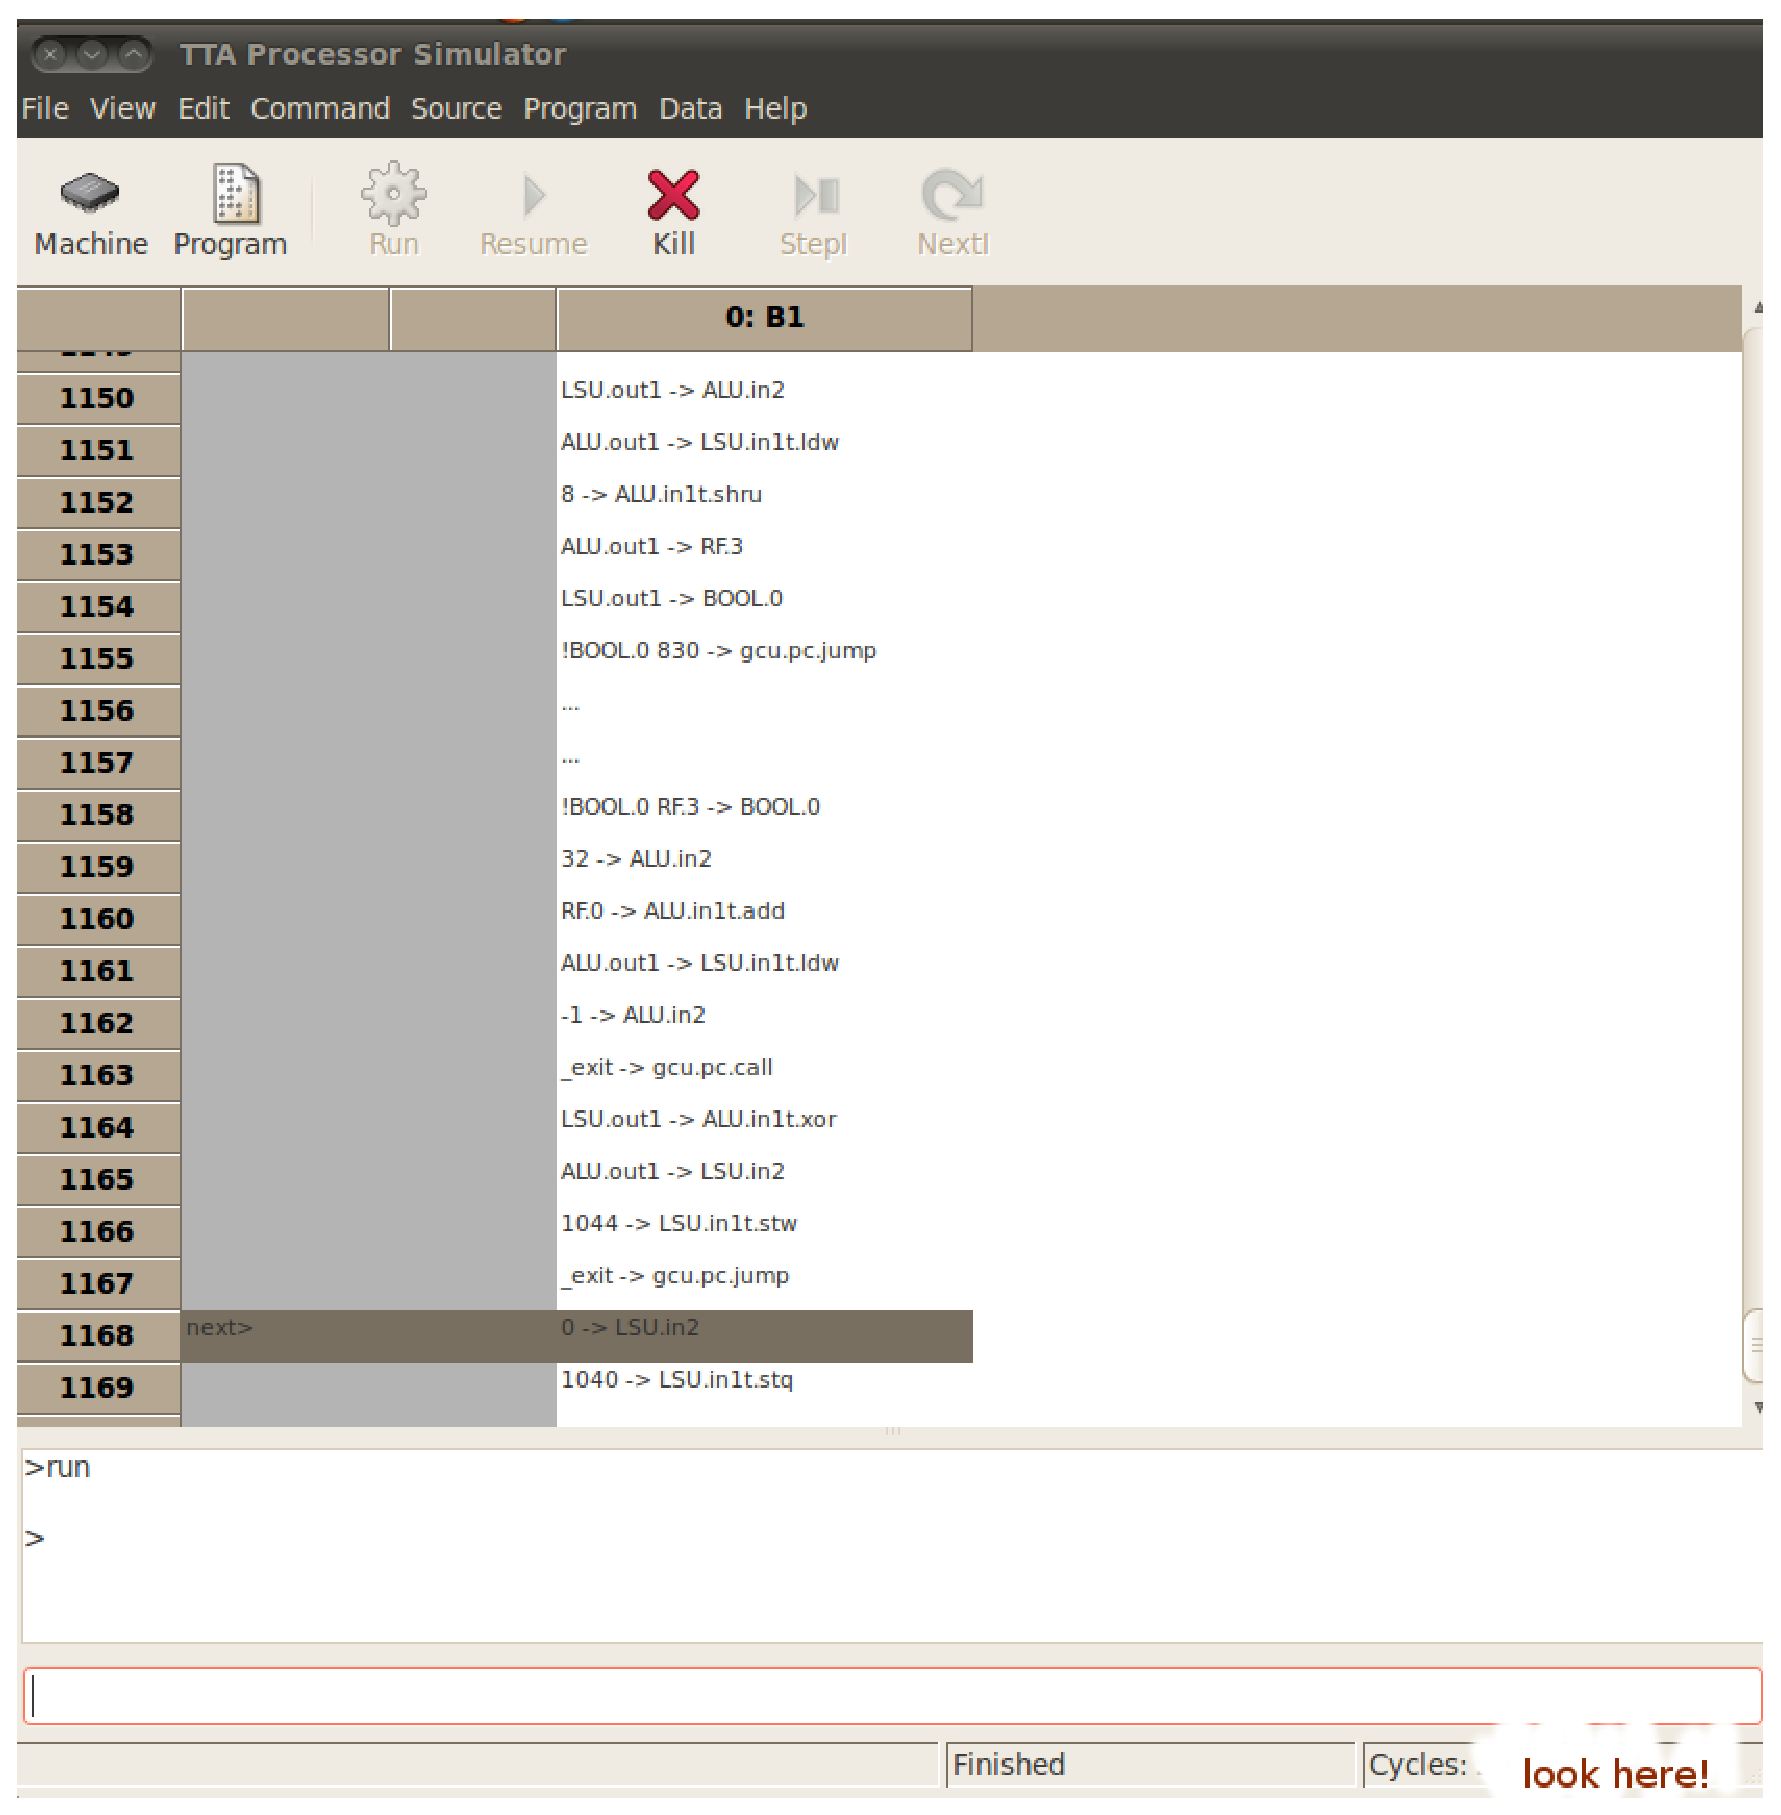
\includegraphics[width=10cm]{eps/proxim_scrshot.eps}
    \caption{Processor Simulator (proxim) when minimal ADF 
             and crc.tpef are opened and simulated.}
    \label{fig:proxim}
  \end{center}
\end{figure}

You can check the result straight from the processor's memory by writing this
command to the command line at the bottom of the simulator:

\shellcmd{x /u w result}

The correct checksum result is \textbf{0x62488e82}.

Processor resource utilization data can be viewed with command:

\shellcmd{info proc stats}

This will output a lot of information like the utilization of transport buses,
register files and function units, for example: 

\begin{verbatim}
utilizations
------------
buses:
B1              87.7559% (4415 writes)

sockets:
lsu_i1          17.4319% (877 writes)
lsu_o1          10.4949% (528 writes)
...

operations executed in function units:
LSU:
...
TOTAL           17.4319% (877 triggers)

ALU:
...
TOTAL           25.2037% (1268 triggers)
...

register accesses:
RF:
0               855 reads,     0 guard reads,      1 writes       
...

\end{verbatim}

Your output may vary depending on the compiler version, the optimizations
used and your architecture.

Proxim can also show othes various pieces of information about the
program's execution and its processor resource utilization. For
example to check the utilization of the resources of our architecture,
select \textit{View>Machine Window} from the top menu. The parts of
the processor that are utilized the most are visualized with darker
red color.

% Next, check the profiling data to see which instructions were executed the
% most. Select: \textit{Source>Profile data>Highlight Top Execution Counts}.
% Now the disassembly window has the most executed instructions highlighted.
% You should be able to spot the main loop of the program easily.
\begin{figure}
  \begin{center}
    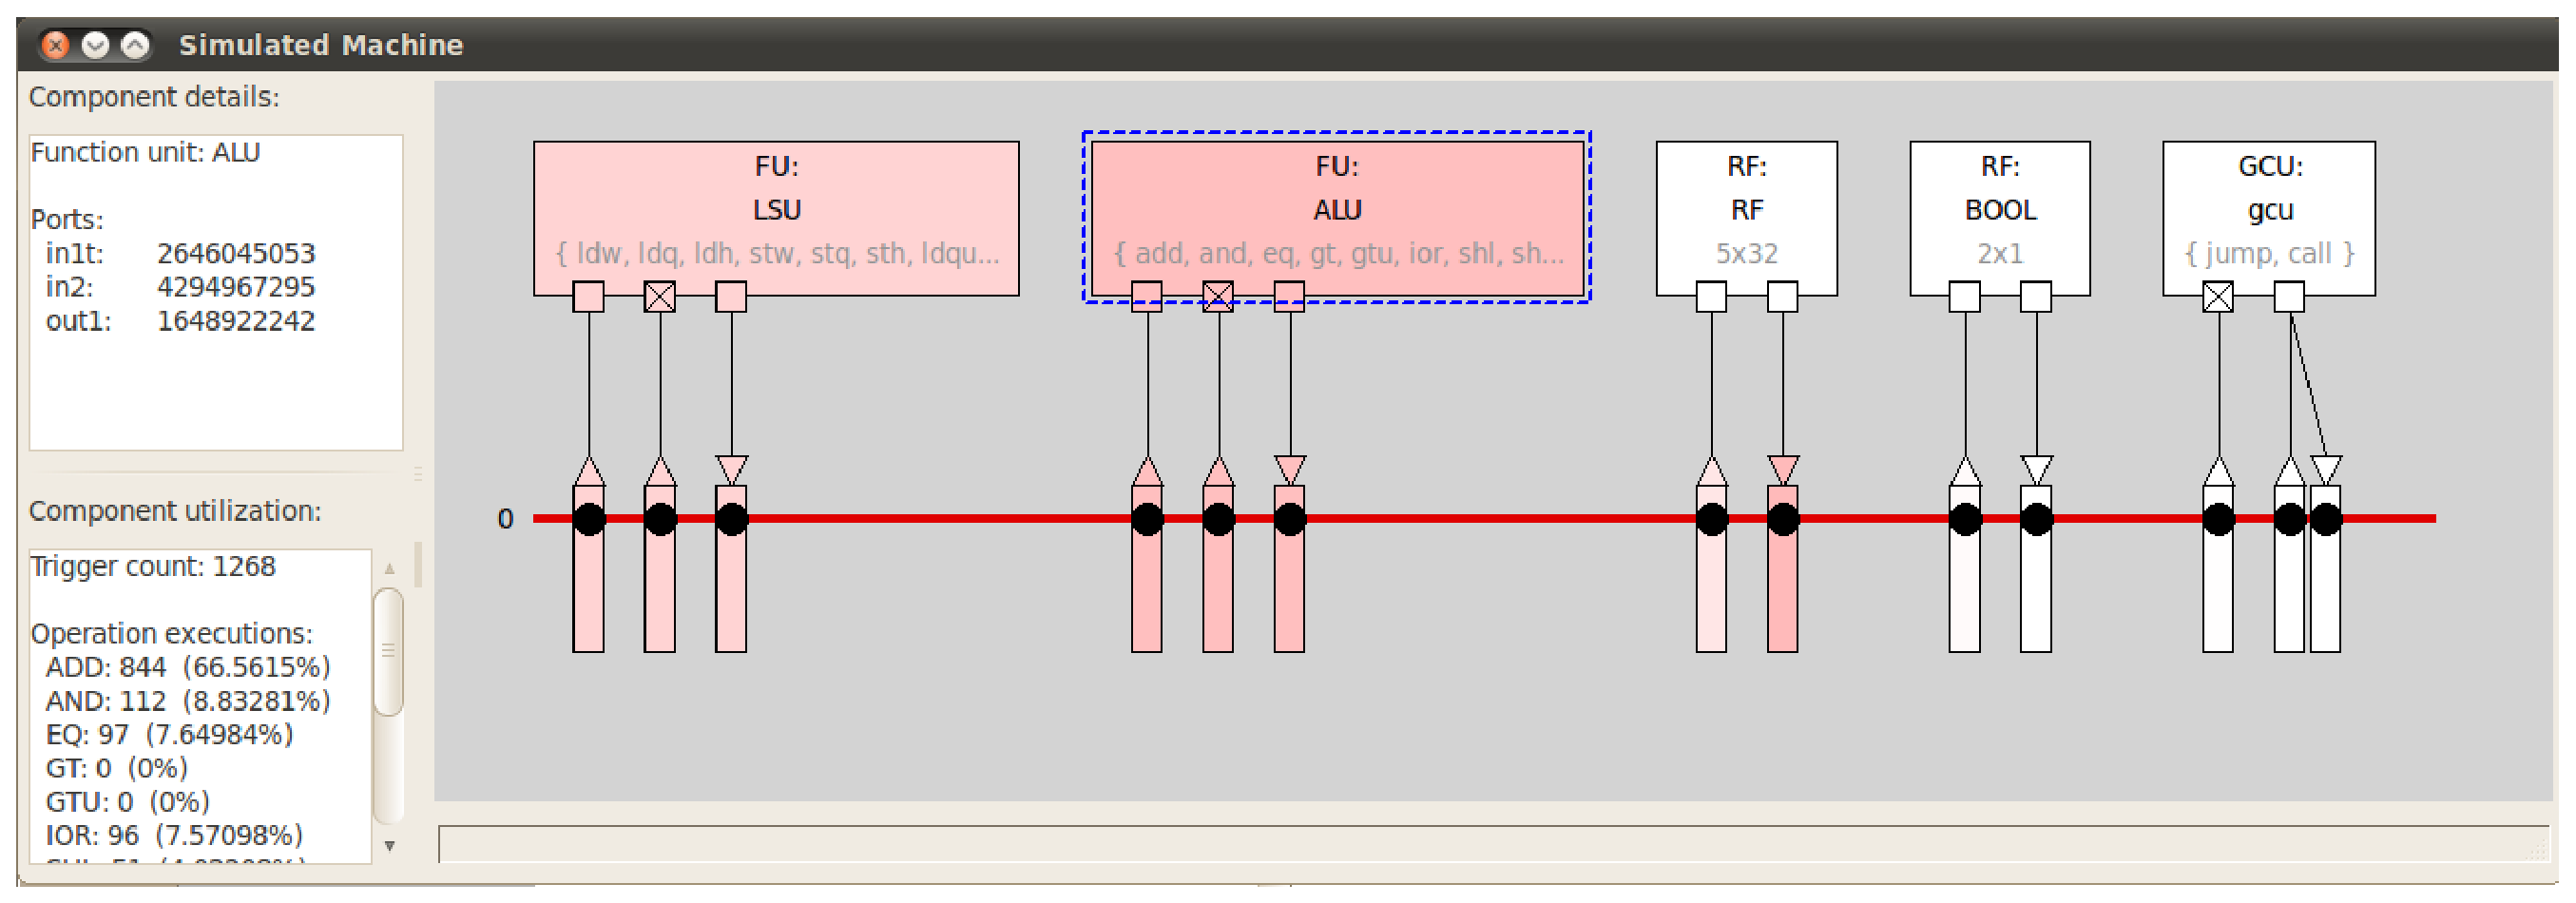
\includegraphics[width=0.7\textwidth]{eps/proxim_util.eps}
    \caption{Processor Simulator (proxim) shows the utilizations of each FU and bus.}
    \label{fig:proxim_util}
  \end{center}
\end{figure}


\begin{table}[b]
  \begin{center}
    \caption {Cycle counts in different TTA configurations. You'll fill this during the tutorial}
    \label {tab:cyclecounts}
    \begin{tabular}{l  l r |  l l }
      \hline
          &             & Approx. relative &            &          \\
      ADF & Cycle count & cycle count      & Section(s) &  Comment \\
      \hline
      \hline
      start.adf            &  & $1~~$  & \ref{ssec:eval_start} & \\ % % 5031 cycles
      \hline
      large.adf            &  & $1/2~$ & \ref{ssec:large} & start + 3 buses \\ % 2383 cycles
      large.adf            &  & $1/5~$ & -''-             & start + 3 buses + RF \\% 935 cycles
      large.adf            &  & $1/6~$ & -''-             & start + 3 buses + RF + new ALU \\ % 778 cycles
      \hline
      custom.adf           &  & $1/5~$ & \ref{ssec:anal_custom} - \ref{ssec:tcetour_final_products} \\ % 958 cycles
      \hline
      large\_custom.adf    &  & $1/50$ & \ref{ssec:large_custom} \\ % 100 cycles! wow!
      \hline
    \end{tabular}
  \end{center}
\end{table}



There are 3 basic ways to accelerate computation in TTAs:
\begin{enumerate}
\item Modify the algorithm itself. Beyond the scope of this tutorial.
\item Add more basic resources (FUs, RFs, buses) to TTA
\item Add custom operation(s) to TTA
\end{enumerate}


\subsection{Increasing performance by adding resources}
\label{ssec:large}
As the current architecture is minimalistic we can increase the performance
even further by adding resources to the processor.

\paragraph{Transport buses.} 
The architecture has only one transport bus, thus the compiler can't exploit 
any instruction level parallelism. Let's start the architecture customization by 
adding another transport bus. After this there can be 2 moves per clock cycle. 
First copy the current architecture:

\shellcmd{cp start.adf large.adf}

and open the new architecture in ProDe:

\shellcmd{prode large.adf \&}

A new transport bus can be added simply by selecting the current bus and
pressing ``ctrl+c'' to copy the bus and then pressing ``ctrl+v'' to paste it.
Add 3 more buses. After you have added the buses you have to connect it to the
sockets. Easiest way to do this is to select ``Tools->Fully connect IC''.
Save the architecture, recompile the source code for the new architecture:

\shellcmd{tcecc -O3 -a large.adf -o crc.tpef -k result crc.c main.c}

This time simulate the program using the command line instruction set simulator:

\shellcmd{ttasim -a large.adf -p crc.tpef}

The command will load the architecture and program and execute
it. Once the simulation is finished, you should see the ttasim command prompt:

\begin{verbatim}
> ttasim -a large.adf -p crc.tpef

(ttasim) 
\end{verbatim}

Now when you check the cycle count from the simulator:

\shellcmd{info proc cycles}

You might see a significant drop in cycles. 
% approx 50% reduction to 2383 cycles
Also check the processor utilization statistics from the simulator
with command:

\shellcmd{info proc stats}

\paragraph{Register files.}

From the previous simulator statistics you can see from ``operations'' table
that there are a lot of load and store operations being executed. As the
architecture has only 5 general purpose registers this tells us that there
are a lot of register spilling to memory. Let's try how the amount of registers affect
the cycle count. There are two options how we can add registers. We can either
increase the number of registers in a register file or add a new register file.

Let's try the latter option because this way we increase the number of registers
that can be accessed simultaneously on one clock cycle. This can be done by
selecting the RF and using copy and paste. Then connect it to the IC.
Simulation statistics should indicate performance increase. As expected, the
number of load and store opertations decreased. But notice also that the number
of add operations decreased quite a lot. The reason is simple: addition is used
to calculate stack memory addresses for the spilled registers.
% over 50% further reduction to 935 cycles

\paragraph{Function units.}
Next subject for the bottleneck is the ALU as now all the basic operations
are performed in a single function unit. From the simulator statistics you can
see that logical operations and addition are quite heavily utilized. Instead
of duplicating the ALU let's add more specific FUs from the Hardware Database.
Select ``Edit->Add From HDB->Function Unit...''. Select a FU which has
operations and(1), ior(1), xor(1) and click ``Add''. Then select FU with operation
add(1) and click ``Add''. Close the dialog, connect the function units and save the
architecture. Recompile and simulate to see the effect on cycle count.
% about 20 further reduction to 778 cycles

The architecture could be still modified even further to drop the cycle count
but let's settle for this now and move on to custom operations. 


\subsection{Analyzing the Potential Custom Operations}
\label{ssec:anal_custom}
%\subsection{Accelerating the CRC Algorithm}
Custom operations implement application specific functionality in TTA
processors. This part of the tutorial teaches how to accelerate the
CRC computation by adding a custom operation to the starting point
processor design.

%\subsubsection{Evaluating Custom Operation Candidates}

First of all, it is quite simple and efficient to implement CRC
calculation entirely on hardware. Naturally, using the whole CRC
function as a custom operation would be quite pointless and the
benefits of using a processor based implementation would get
smaller. Instead, we will concentrate on trying to accelerate
smaller parts of the algorithm, which is the most useful way for most
algorithms.

 The steps needed for custom opeation are:
\begin{enumerate}
\item Analyze the code for bottlenecks

\item Speculatively add a new module and operation to operation
  database with OSEd. Define the behavior of the new operation
  (copy-paste from original code and add few macros). Optionally, you
  can also simulate the operation behavior. Bind the new operation to
  a new function unit in ProDe

\item Modify your source code so that it utilizes the new operation
  and simulate. Go back to step 2 if you wish to explore other
  operations

\item Create VHDL for the operation and add it to HDB.
 
\item Finally, generate HDL implementation of the TTA with ProGe.
\end{enumerate}
%\subsubsection{Finding the Bottlenecks}

% The first thing to do when trying to optimize code is to profile the execution.
% In Proxim you can trace the most executed instructions (see section
% \ref{sec:ProfileProxim} for more information). Another way to produce 
% program profile data is to enable
% ``setting profile\_data\_saving 1'' in ttasim before initializing the simulation.
% This produces a crc.tpef.trace file from which one can dump the function
% profile using a command ``dump\_function\_profile crc.tpef.trace''. 
% A call profile helps locating the functions that are executed the most. 
% Refer to section \ref{sec:traces} for further
% information.

Finding the operation to be optimized is quite obvious in this case if
you look at function crcFast(). It consists of a for-loop in which the
function reflect() is called through the macro REFLECT\_DATA. If you
look at the actual function (shown also in Fig.~\ref{fig:reflect} you
can see that it is quite simple to implement on hardware, but requires
many instructions if done with basic operations in software. The
function ``reflects'' the bit pattern around the middle point like a
mirror. For example, the bit pattern \textbf{1101 0010} becomes
\textbf{0100 1011}. The main complexity of the function is that the bit 
pattern width is not fixed. Fortunately, the width cannot be
arbitrary. If you examine the crcFast()-function and the reflect
macros you can spot that function reflect() is only called with 8 and
32 bit widths (unsigned char and 'crc' which is an unsigned long).

%\subsection{Analyzing the Custom Operation}

A great advantage of TCE is that the operation semantics, processor
architecture, and implementation are separate abstractions. This
simplifies designing custom operations since you can simulate your
design by simply defining the simulation behaviour of the operation
and setting the latency of the operation to the processor architecture
definition. This is nice as you do not need an actual hardware
implementation of the operation at this point of the design, but can
evaluate different custom operation possibilities at the architectural
level. However, this brings up an awkward question: how to determine
the latency of the operation? Unrealistic or too pessimistic latency
estimates can produce inaccurate performance results and bias the
analysis.

One approach to the problem is to take an educated guess and simulate
some test cases with different custom operation latencies. This way
you can determine a latency range in which the custom operation would
accelerate your application to the satisfactory level. For example,
custom operation with 1 cycle delay might give $3x$ speedup but $10$
cycles gives just 3\%.  After this you can sketch how the operation
could be implemented in hardware, or consult someone knowledgeable in
hardware design to figure out whether the custom operation can be
reasonably implemented within the latency constraint.

\begin{figure}
  \begin{center} 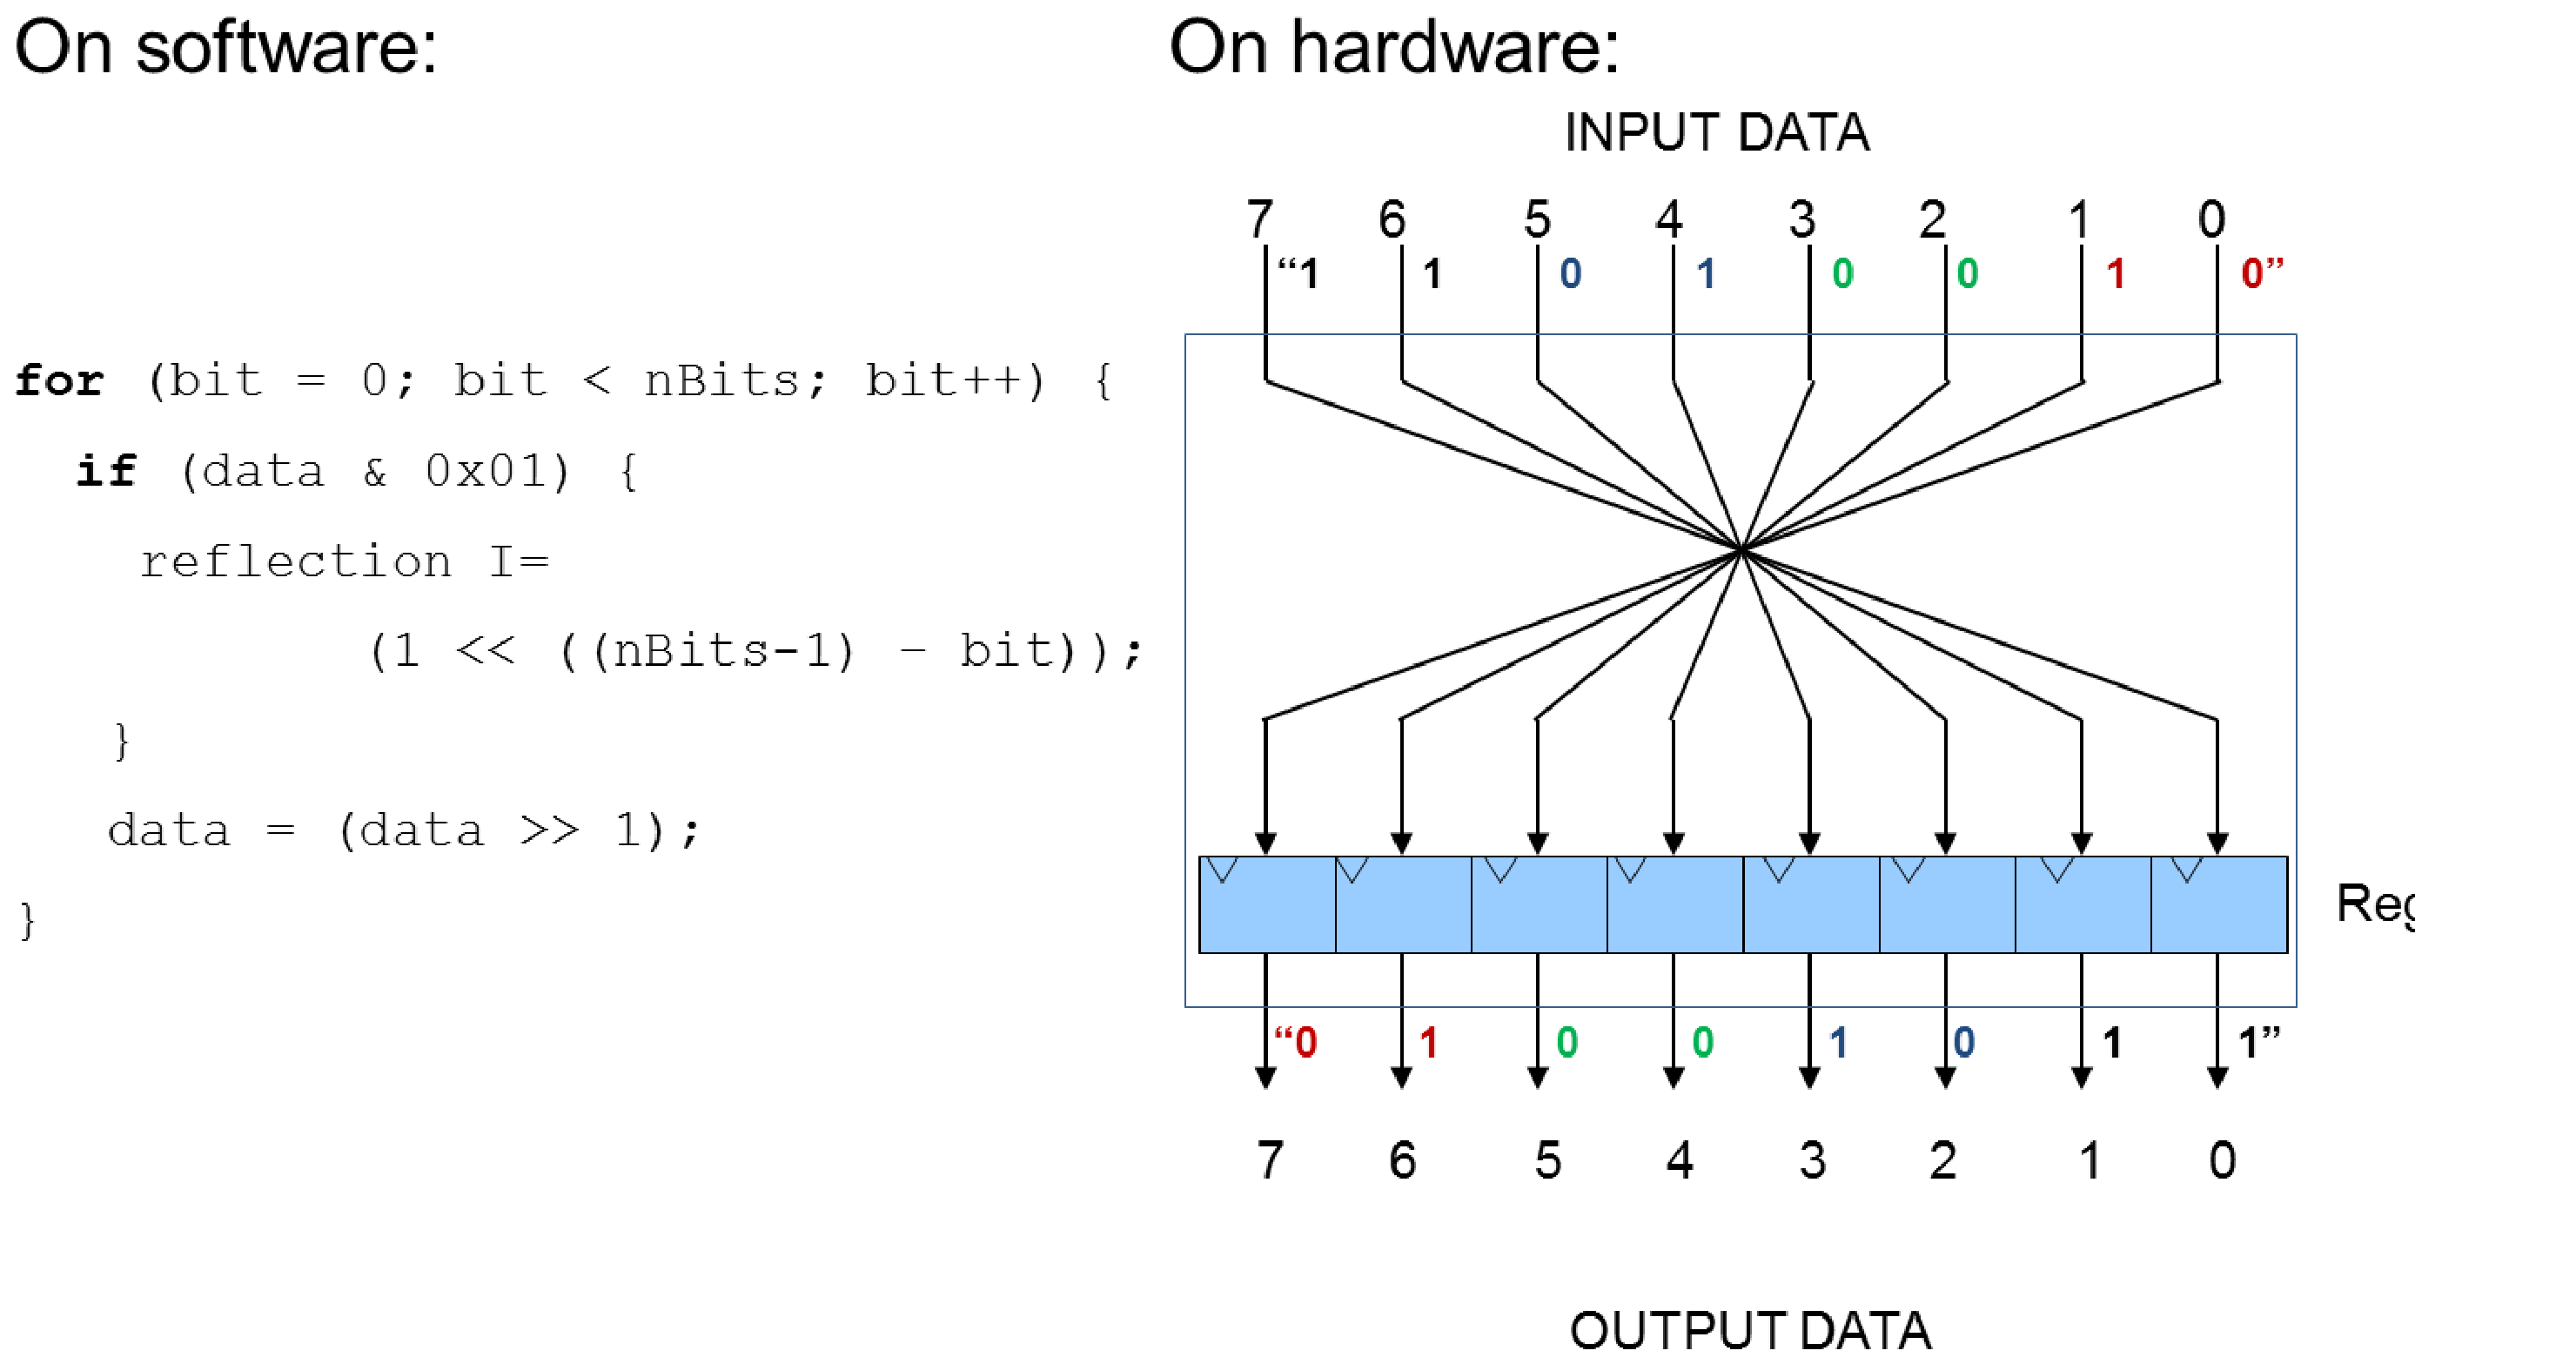
\includegraphics[width=0.8\textwidth]{eps/reflect}
  \caption{Reflect function of CRC} 
  \label{fig:reflect} \end{center}
\end{figure}

Another approach is to try and determine the latency by examining the
operation itself and considering how it could be implemented. This
approach requires some insight in digital design.

Besides latency you should also consider the size of the custom
function unit.  It will consume extra die area, but the size limit is
always case-specific, especially when area taken by memories is
accounted. Accurate size estimation requires the actual HW
implementation and synthesis.

Let us consider the reflect function. If we had fixed width we could
implement the reflect by hard wiring (and registering the output)
because the operation only moves bits to other locations in the
word. This could be done easily in one clock cycle, as in right side
of Fig.~\ref{fig:reflect}. But we need two different bit widths so it
is somewhat more complicated. We could design the HW in such way that
it has two operations: one for 8-bit data and another for 32-bit
data. One way to implement this is to have 32-bit wide crosswiring and
register the output. The 8-bit value would be reflected to the 8 MSB
bits of the 32-bit wiring. Then we need to move the 8 MSB bits to the
LSB end and set rest to zero. This moving can be implemented using
multiplexers. So concerning the latency this can all be done easily
within one clock cycle as there is not much logic needed.




\subsection{Creating the Custom Operation}
\label{section:customOperations}
% includes adding a FU that implements the custom operation to HDB and
% adding the operation to OSAL

Now we have decided the operation to be accelerated and its
latency.


Next we will create a function unit implementing the
operation and add it to our processor design. First, a description of
the semantics of the new operation must be added at least to Operation
Set Abstraction Layer (Sections~\ref{section:osal} and
\ref{section:osal_details}). OSAL stores the semantic properties of
the operation, which includes the simulation behavior, operand count
etc., but not the latency. OSAL definitions can be added by using the
OSAL GUI, \emph{OSEd} (Section~\ref{sec:osed}).

Synthesis or simulation at the VHDL level requires that at least one
function unit implementing the operation must be added to the Hardware
Database (Section~\ref{section:hdb}).  In this tutorial we add the FU
implementation for our custom operation so the processor
implementation can be generated, but omit the cost data required for
the cost estimation. In general case, cost data should be added to
cost database as well.

\paragraph{Using Operation Set Editor (OSEd) to add the operation data.}

OSEd is started with the command 

\shellcmd{osed \&}

Create a new operation module, which is a container for a set of
operations.  You can add a new module in any of the predefined search
paths, provided that you have sufficient file system access
permissions.

For example, choose directory
\file{/home/\emph{user}/.tce/opset/custom}, where \emph{user} is the
name of the user account being used for the tutorial.  This directory
is intended for the custom operations defined by the current user, and
should always have sufficient access rights.

\begin{figure}
  \begin{center} 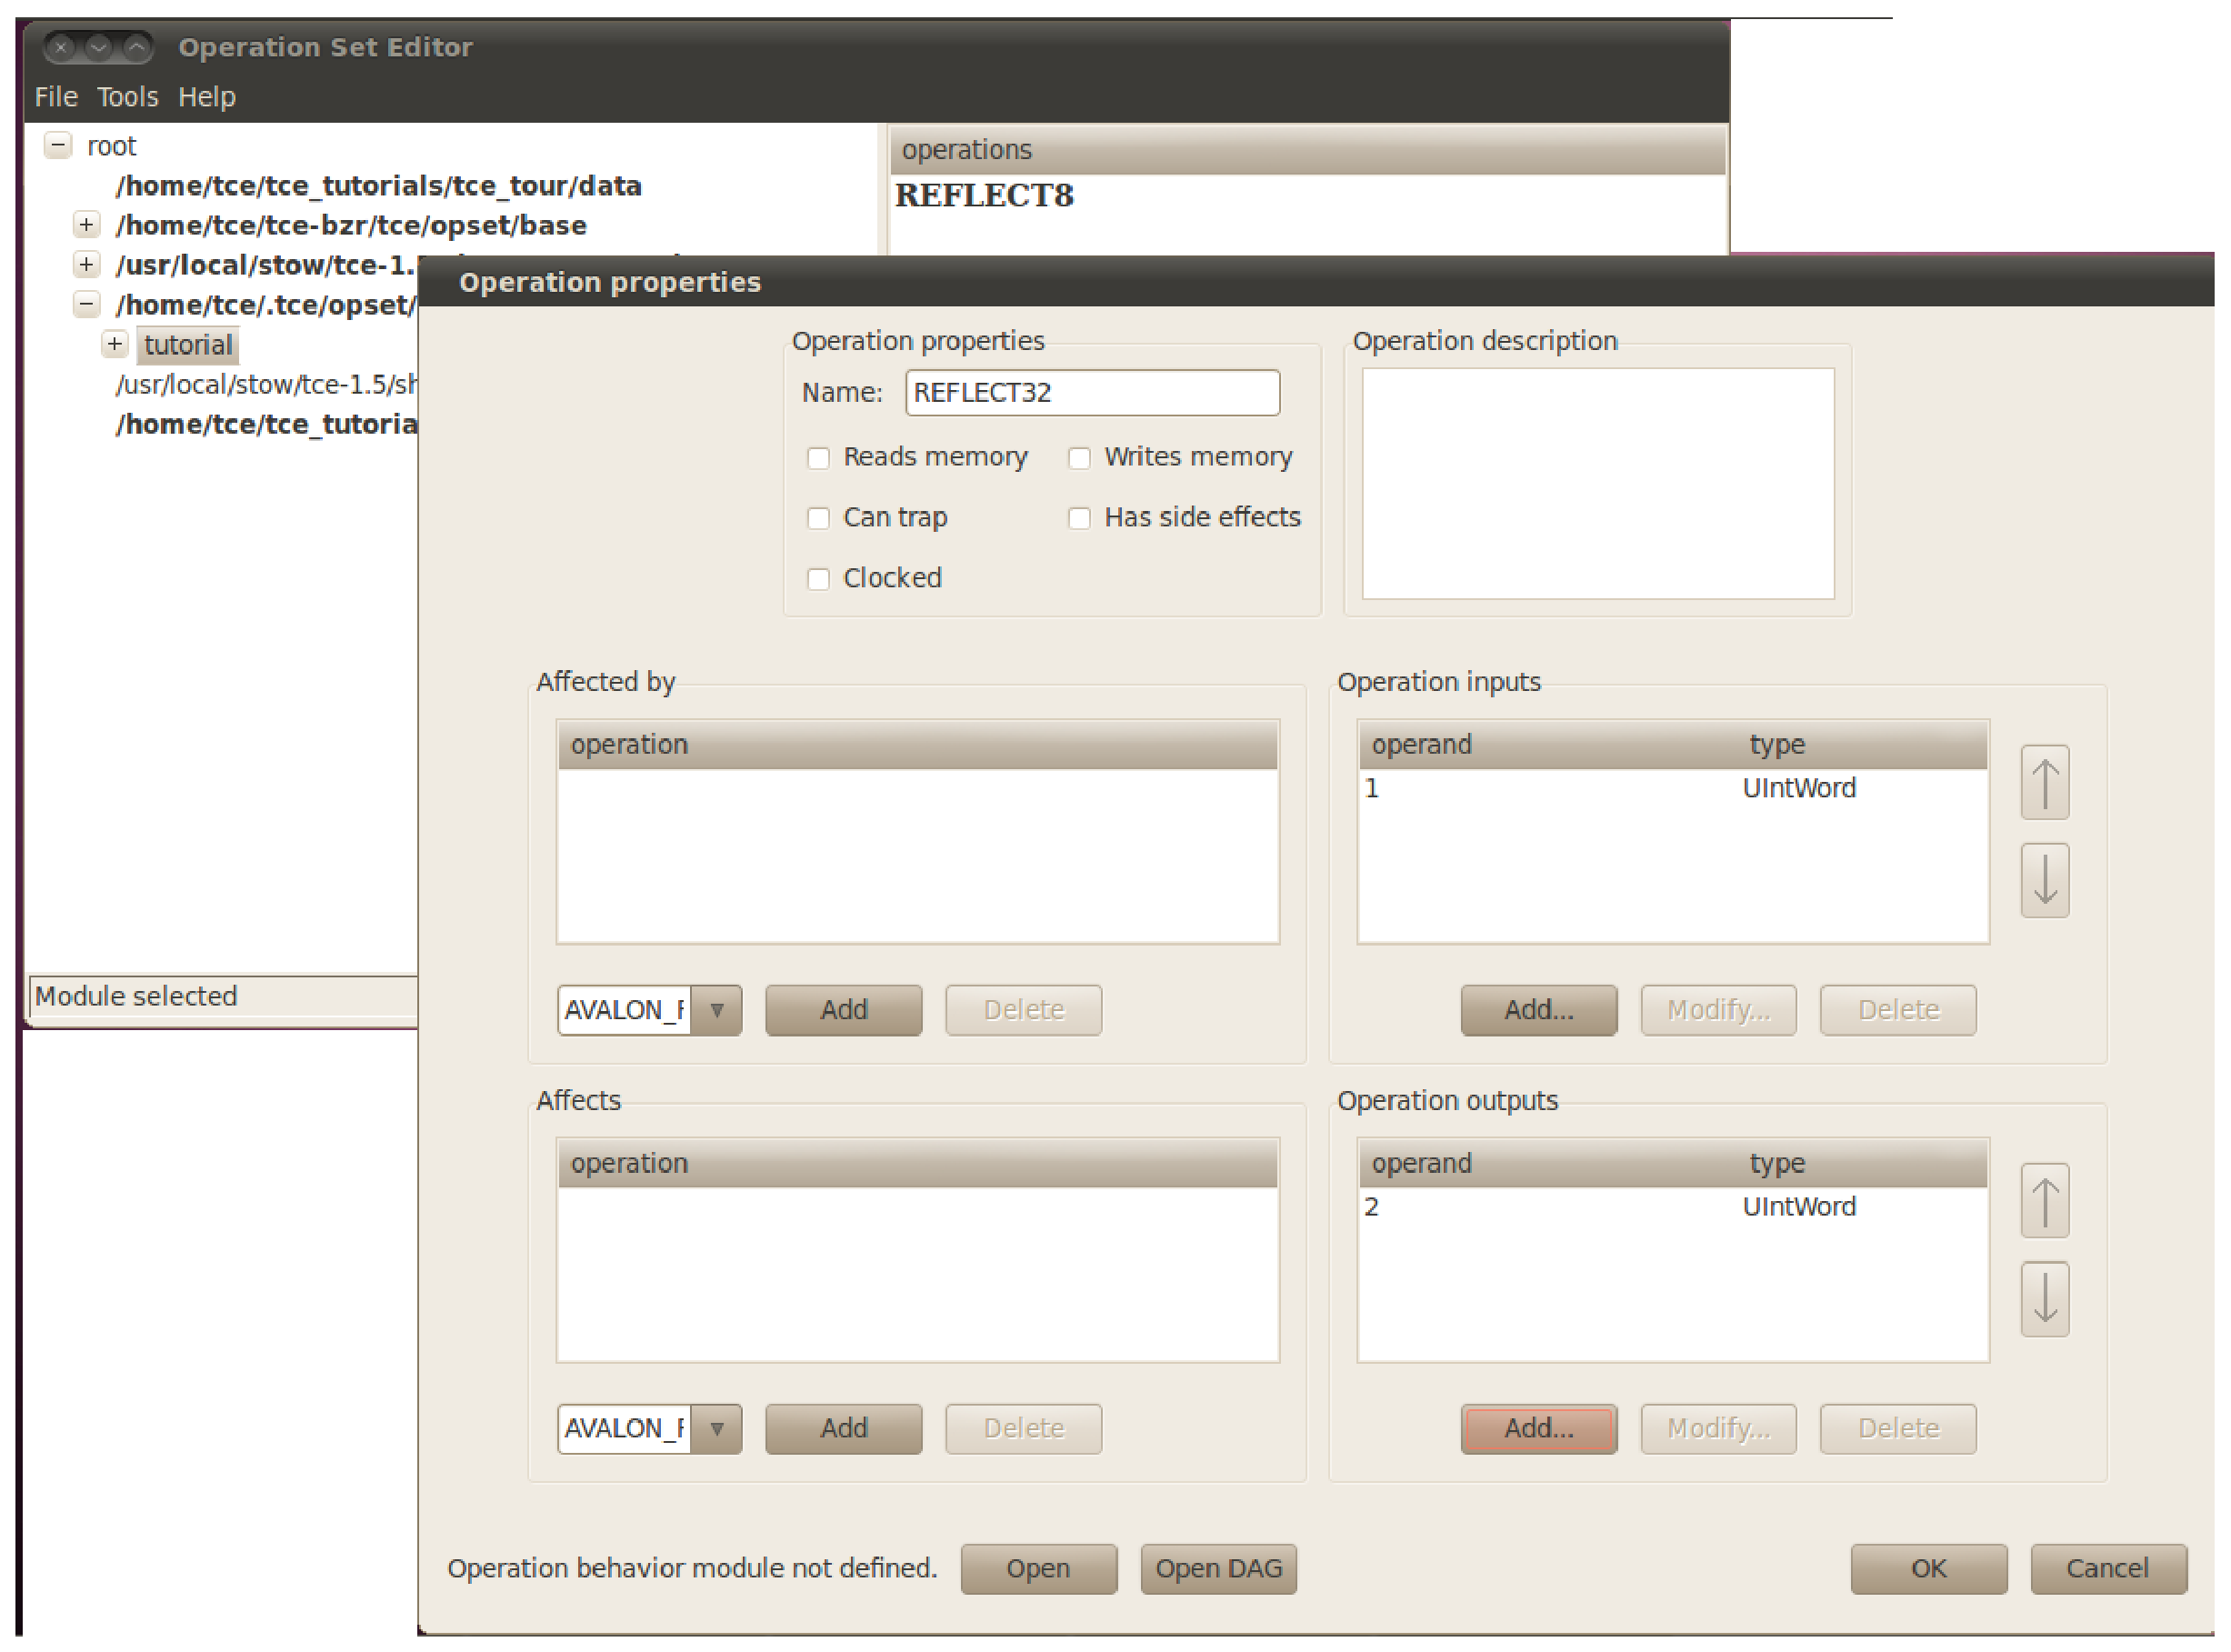
\includegraphics[width=0.8\textwidth]{eps/osed}
  \caption{Operation Set Editor when adding new operation REFLECT32.} 
  \label{fig:osed} \end{center}
\end{figure}


\begin{enumerate}
\item%
  Click the root in the left area of the main window which opens list
  of paths. Right-click on a path name
  \file{/home/\emph{user}/.tce/opset/custom}. A drop-down menu appears
  below the mouse pointer.
\item%
  Select \textbf{Add module} menu item. 
\item%
  Type in the name of the module (for example, `tutorial') and press \emph{OK}.
  The module is now added under the selected path.
\end{enumerate} 

\paragraph{Adding the new operations.} We will now add the operation
definitions to the newly created operation module.

\begin{enumerate}
\item%
  Select the module that you just added by right-clicking on its name,
  displayed in the left area of the main window. A drop down menu appears.
\item%
  Select \textbf{Add operation} menu item.
\item%
  Type `REFLECT8' as the name of the operation.
\item%
  Add one input by pressing the \emph{Add} button under the operation input
  list. Select \textit{UIntWord} as type.
\item%
  Add one output by pressing the \emph{Add} button under the operation output
  list. Select \textit{UIntWord} as type.
\item%
  After the inputs and the output of the operation have been added, close
  the dialog by pressing the \emph{OK} button. A confirmation dialog will pop
  up. Press \emph{Yes} to confirm the action. The operation definition is
  now added to the module.
\item%
  Then repeat the steps for operation `REFLECT32', as shown in Fig.~\ref{fig:osed}
\end{enumerate}

\paragraph{Defining the simulation behaviour of the operations} The new operations
REFLECT8 and REFLECT32 do not yet have simulation behavior models, so
we cannot simulate programs that use these operations with the TCE
processor simulator. Open again the operation property dialog by
right-clicking REFLECT8, then choosing \emph{Modify properties}. Now
press the \emph{Open} button at the bottom to open an empty behavior
source file for the module. Copy-paste (or type if you have the time!) 
the following code in the editor window:

\begin{verbatim}
#include "OSAL.hh"
OPERATION(REFLECT8)
 TRIGGER

 unsigned long data = UINT(1);
 unsigned char nBits = 8;

 unsigned long  reflection = 0x00000000;
 unsigned char  bit;

 /*
  * Reflect the data about the center bit.
  */
 for (bit = 0; bit < nBits; ++bit)
 {
     /*
      * If the LSB bit is set, set the reflection of it.
      */
     if (data & 0x01)
     {
         reflection |= (1 << ((nBits - 1) - bit));
     }

     data = (data >> 1);
 }

 IO(2) = static_cast<unsigned> (reflection);

 return true;
 END_TRIGGER;
 END_OPERATION(REFLECT8)

OPERATION(REFLECT32)
 TRIGGER

 unsigned long data = UINT(1);
 unsigned char nBits = 32;

 unsigned long  reflection = 0x00000000;
 unsigned char  bit;

 /*
  * Reflect the data about the center bit.
  */
 for (bit = 0; bit < nBits; ++bit)
 {
     /*
      * If the LSB bit is set, set the reflection of it.
      */
     if (data & 0x01)
     {
         reflection |= (1 << ((nBits - 1) - bit));
     }

     data = (data >> 1);
 }

 IO(2) = static_cast<unsigned> (reflection);

 return true;
 END_TRIGGER;
 END_OPERATION(REFLECT32)
\end{verbatim}

This code has the behaviours for the both operations. These behavior
definitions reflect the input operand integer (id 1, assigned to
variable 'data') and writes the result to the ''output operand`` (id
2, assigned from variable 'reflection') which is the first output and
signals the simulator that all results are computed successfully.

Open file \file{crc.c} in your preferred editor. Compare the behaviour
definition of reflect operations and the original
reflect-function. The function is mostly similar except for parameter
passing and adding few macros added, such as OPERATION(), TRIGGER,
IO(2) etc. Custom hardware operation behavior reads data from the
function unit's input ports and writes to output ports. The value of
nBits is determined from the operation code (REFLECT8 or REFLECT32).

Save the code and close the editor. REFLECT8 and REFLECT32 operations
now have TCE simulator behaviour models.

\paragraph{Compiling operation behavior.} REFLECT-operations have been
added to the test module. Before we can simulate the behavior of our
operation, the C++-based behavior description must be compiled to a plugin
module that the simulator can call.

\begin{enumerate}
\item%
  Right-click on the module name ('tutorial') displayed in the left area to bring up the
  drop down menu.
\item%
  Select \textbf{Build} menu item. 
\item%
  Hopefully, no errors were found during the compilation! Otherwise, re-open
  the behaviour source file and try to locate the errors with the
  help of the diagnostic information displayed in the build dialog.
\end{enumerate}

After the operation simulation model has been added and compiled the operation
can be simulated. But for the sake of speed up we will skip the operation
simulation here. Interested readers are referred to Section~\ref{sec:osed}
You can close osed now.

%  Simulation section removed
% \begin{enumerate}
% \item%
%   Right-click on the operation name displayed in the left area of the
%   main window, under the operation module that contains it.
% \item%
%   Select \textbf{Simulate} menu item from the drop-down menu. 
% \item%
%   Edit the input values of REFLECT8 (or REFLECT32) by selecting the input
%   operand from the list and typing the values in the text input field and
%   pressing the \emph{Update} button next to the field. In this case it is
%   handy to choose the format to be binary.
% \item%
%   Press the \emph{Trigger} button. The value of the output should be updated.
% \item%
%   The format of the displayed input and output values can be modified by
%   selecting different formats from the choice list next to the label
%   `Format:'. It might be more illustrating if you change input and output
%    format to binary.  This way we can enter binary patterns, 
%    for example '11001100' (as binary) for the first operand. The trigger
%    should produce the reflected value '00110011' for operation REFLECT8
% 
% \item%
%   The state of operation can be reset by pressing the \emph{Reset} button.
% \item%
%   Repeat the test with different input values. After you are convinced
%   the behavior definition works, close the dialog by clicking on the \emph{OK} button.
% \end{enumerate}

\paragraph{Adding a Customized Function Unit to the Architecture.}

Now the operation definitions of the custom operations have been added to the
Operation Set Abstraction Layer (OSAL) database. Next we need to add at
least one functional unit (FU) which implements these operations so that they
can be used in the processor design. Note the separation between ''operation`` and
an ''function unit`` that implements the operation(s) which allows using the
same OSAL operation definitions in multiple FUs with different latencies.

First, add the architecture of the FU that implements the custom operations
to the starting point processor architecture. Let's take a copy of the starting
point processor design which we can freely modify and still be able to easily
compare the architecture with and without the custom operation support later on:

\shellcmd{cp start.adf custom.adf}

Open the copy in ProDe:

\shellcmd{prode custom.adf \&}

\begin{figure}
  \begin{center} 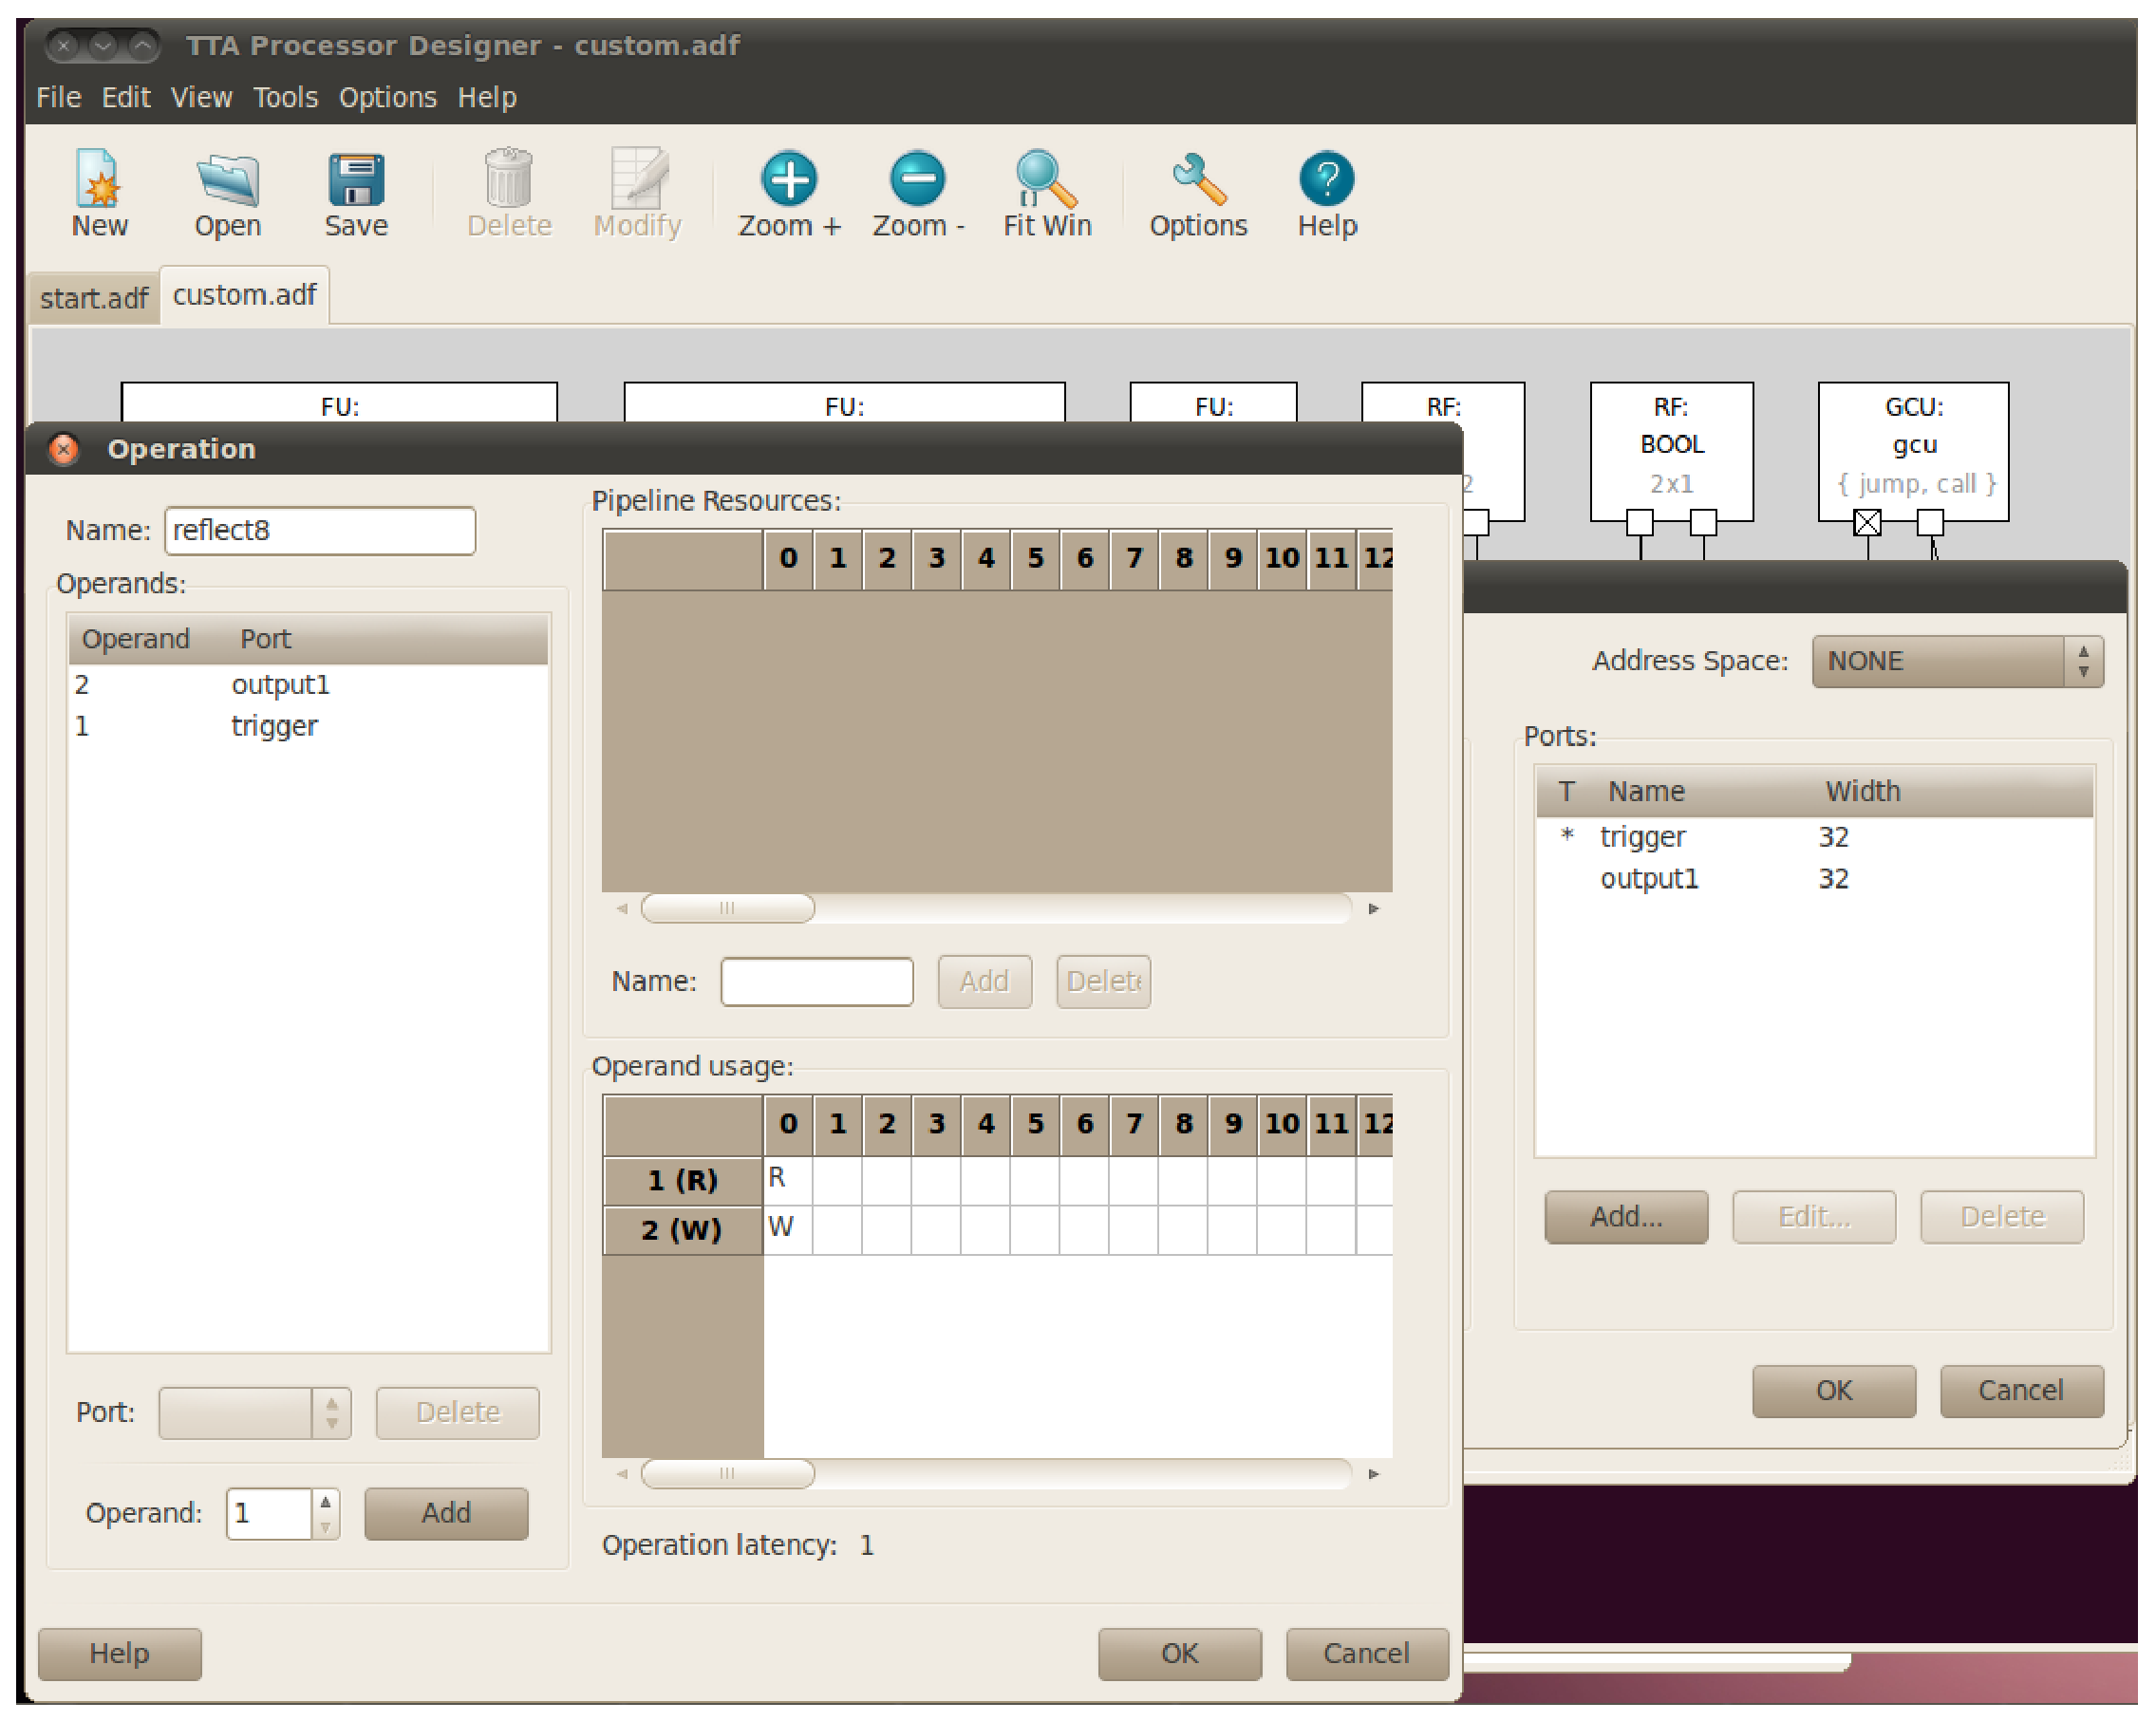
\includegraphics[width=0.8\textwidth]{eps/reflecter}
  \caption{Adding operation REFLECT8 to a new function unit in ProDe} 
  \label{fig:reflecter} \end{center}
\end{figure}

Then:
\begin{enumerate}
\item%
  Add a new function unit to the design, right click the canvas and
  select: \textit{Add>Function Unit}. Name the FU ''REFLECTER``. Add
  one input port (named as trigger) and an output port (output1) to
  the FU in the Function unit dialog. Set the input port (trigger)
  triggering (\textit{Click the port named trigger->Edit->Check dialog
    ''triggers``}). This port starts the execution of the operation
  when it is written to.
\item%
  Add the operation ''REFLECT8`` we defined to the FU: \textit{Add
    from opset>REFLECT8>OK} and set the latency to 1. Click on the
  REFLECT8 operation and ensure that the operation input is bound to
  the input ports and the output is bound to the output port. Check
  that the operand usage is in such a way that input is read at cycle
  0 and the result is written at the end of the cycle (can be read
  from the FU on the next cycle), as in
  Fig.~\ref{fig:reflecter}. Thus, the latency of the operation is 1
  clock cycles.
\item%
  Repeat the previous step for operation ''REFLECT32``
\item%
  Now an FU that supports the custom operations has been added to the
  architecture. Next, connect the FU to the rest of the
  architecture. This can be most easliy done by selecting
  \textit{Tools->Fully Connect IC} which connects all FUs to all the
  buses. Save the architecture description by clicking Save.
\end{enumerate}


\subsection{Use the custom operation in C code.}

To get some benefits from the added custom hardware, we must use it
from the C code. This is done by replacing a C statement with a custom
operation invocation.

Let us first backup the original C code.

\shellcmd{cp crc.c crc\_with\_custom\_op.c}

Then open \file{crc\_with\_custom\_op.c} in your preferred text editor.

\begin{enumerate}
\item%
Add \#include ``tceops.h'' to the top of the file. This includes 
automatically generated macros which allow us to use specific 
operations from C code without getting our hands dirty with
inline assembly.

Usage of these macros is as follows:

\begin{verbatim}
 _TCE_<opName>(input1, ... , inputN, output1, ... , outputN);
\end{verbatim}

where <opName> is the name of the operation in OSAL. Number of input and 
output operands depends on the operation. Input operands are given first 
and they are followed by output operands if any. 

In our case we need to write operands into the reflecter and read the
result from it. We named the operations ``REFLECT8'' and ``REFLECT32'', thus
the macros we are going to use are as follows:

\begin{verbatim}
 _TCE_REFLECT8(input1, output);
 _TCE_REFLECT32(input1, output);
\end{verbatim}

Now we will modify the crcFast function to use the custom op.
First declare 2 new variables at the beginning of the function:

\begin{verbatim}
 crc input;
 crc output;
\end{verbatim}

These will help in using the reflect FU macro.

Take a look at the REFLECT\_DATA and REFLECT\_REMAINDER macros. The first one
has got a magic number 8 and ``variable'' X is the data. This is used in the
for-loop of crcFast().

The input data of reflect function is read from array message[] in the for-loop the.
Let us modify this so that at the beginning of the loop the input data is
read to the input variable. Then we will use the \_TCE\_REFLECT8 macro to run
the custom operations, and finally replace the REFLECT\_DATA macro with the
output variable. After these modifications the body of the for-loop should
look like this:

\begin{verbatim}
 input = message[byte];
 _TCE_REFLECT8(input, output);
 data = (unsigned char) output ^ (remainder >> (WIDTH - 8));
 remainder = crcTable[data] ^ (remainder << 8);
\end{verbatim}

Next we will modify the return statement. Originally it uses
REFLECT\_REMAINDER macro where nBits is defined as WIDTH and data is
remainder. Simply use \_TCE\_REFLECT32 macro before return statement and
replace the original macro with the variable output:

\begin{verbatim}
 _TCE_REFLECT32(remainder, output);
 return (output ^ FINAL_XOR_VALUE);
\end{verbatim}

And now we are ready. Remember to save the file.

\item%
Compile the custom operation using C code to a parallel TTA program using the new 
architecture which includes a FU with the custom operation:

\shellcmd{tcecc -O3 -a custom.adf -o crc\_with\_custom\_op.tpef -k result }\verb#\#\\
\shellcmd{\ \ crc\_with\_custom\_op.c main.c}

\item%
Simulate the parallel program. This time we will use the command line simulator
ttasim. We will also enable writing of bus trace. It means that the simulator
writes a text file containing the bus values of the processor from every
executed clock cycle. This bus trace data will be used to verify the processor
RTL implementation. Start the simulator with command:

\shellcmd{ttasim}

Then enable the bus trace setting:

\shellcmd{setting bus\_trace 1}

Load architecture and program and run the simulation

\shellcmd{mach custom.adf}

\shellcmd{prog crc\_with\_custom\_op.tpef}

\shellcmd{run}

Verify that the result is the same as before (\textit{x /u w result}). It
should be the same as earlier (\textbf{0x62488e82}).
Check the cycle count \textit{info proc cycles}  % about 958 cycles
and compare it to the cycle 
count of the version which does not use a custom operation. You should see 
a very noticeable drop compared to the starting point architecture without
the custom operations. Write this cycle count down for a later step and quit ttasim.

The simulator execution also created a file
\file{crc\_with\_custom\_op.tpef.bustrace} which contains the bus
trace.

\end{enumerate}

\subsection{Adding HDL implementation of the FU to the hardware database
(HDB).}
\label{par:AddToHDB}

Now we have seen that the custom operation accelerates our application. Next
we'll add a VHDL implementation of the custom FU to Hardware Database (hdb).
This way we will be able to generate a VHDL implementation of our processor.

If you want to skip this phase you can use the given \file{tour\_example.hdb}
instead of creating it yourself.

Start HDBEditor (see Section~\ref{sec:hdbedit}):

\shellcmd{hdbeditor \&}

TCE needs some data of the FU implementation in order to be able to 
automatically generate processors that include the FU. \\
\begin{enumerate}
 \item% Create a new hdb and name it tour.hdb. Add the ''reflecter``
 function unit from \file{custom.adf} file (\textit{edit->add->FU
 architecture from ADF}).  You can leave the checkboxes ''parametrized
 width`` and ''guard support`` unchecked, which is the default.  Then
 define implementation for the added function unit entry \textit{right
 click reflect -> Add implementation....}\\

\item%
Open file \file{tour\_vhdl/reflect.vhdl} that was provided in the tutorial
package with the editor  you prefer, and take a look. This is an example
implementation of  a TTA function unit performing the custom 'reflect8'
and 'reflect32' operations.

%!!! VHDL needs comments and a header !!!
\begin{figure}
  \begin{center} 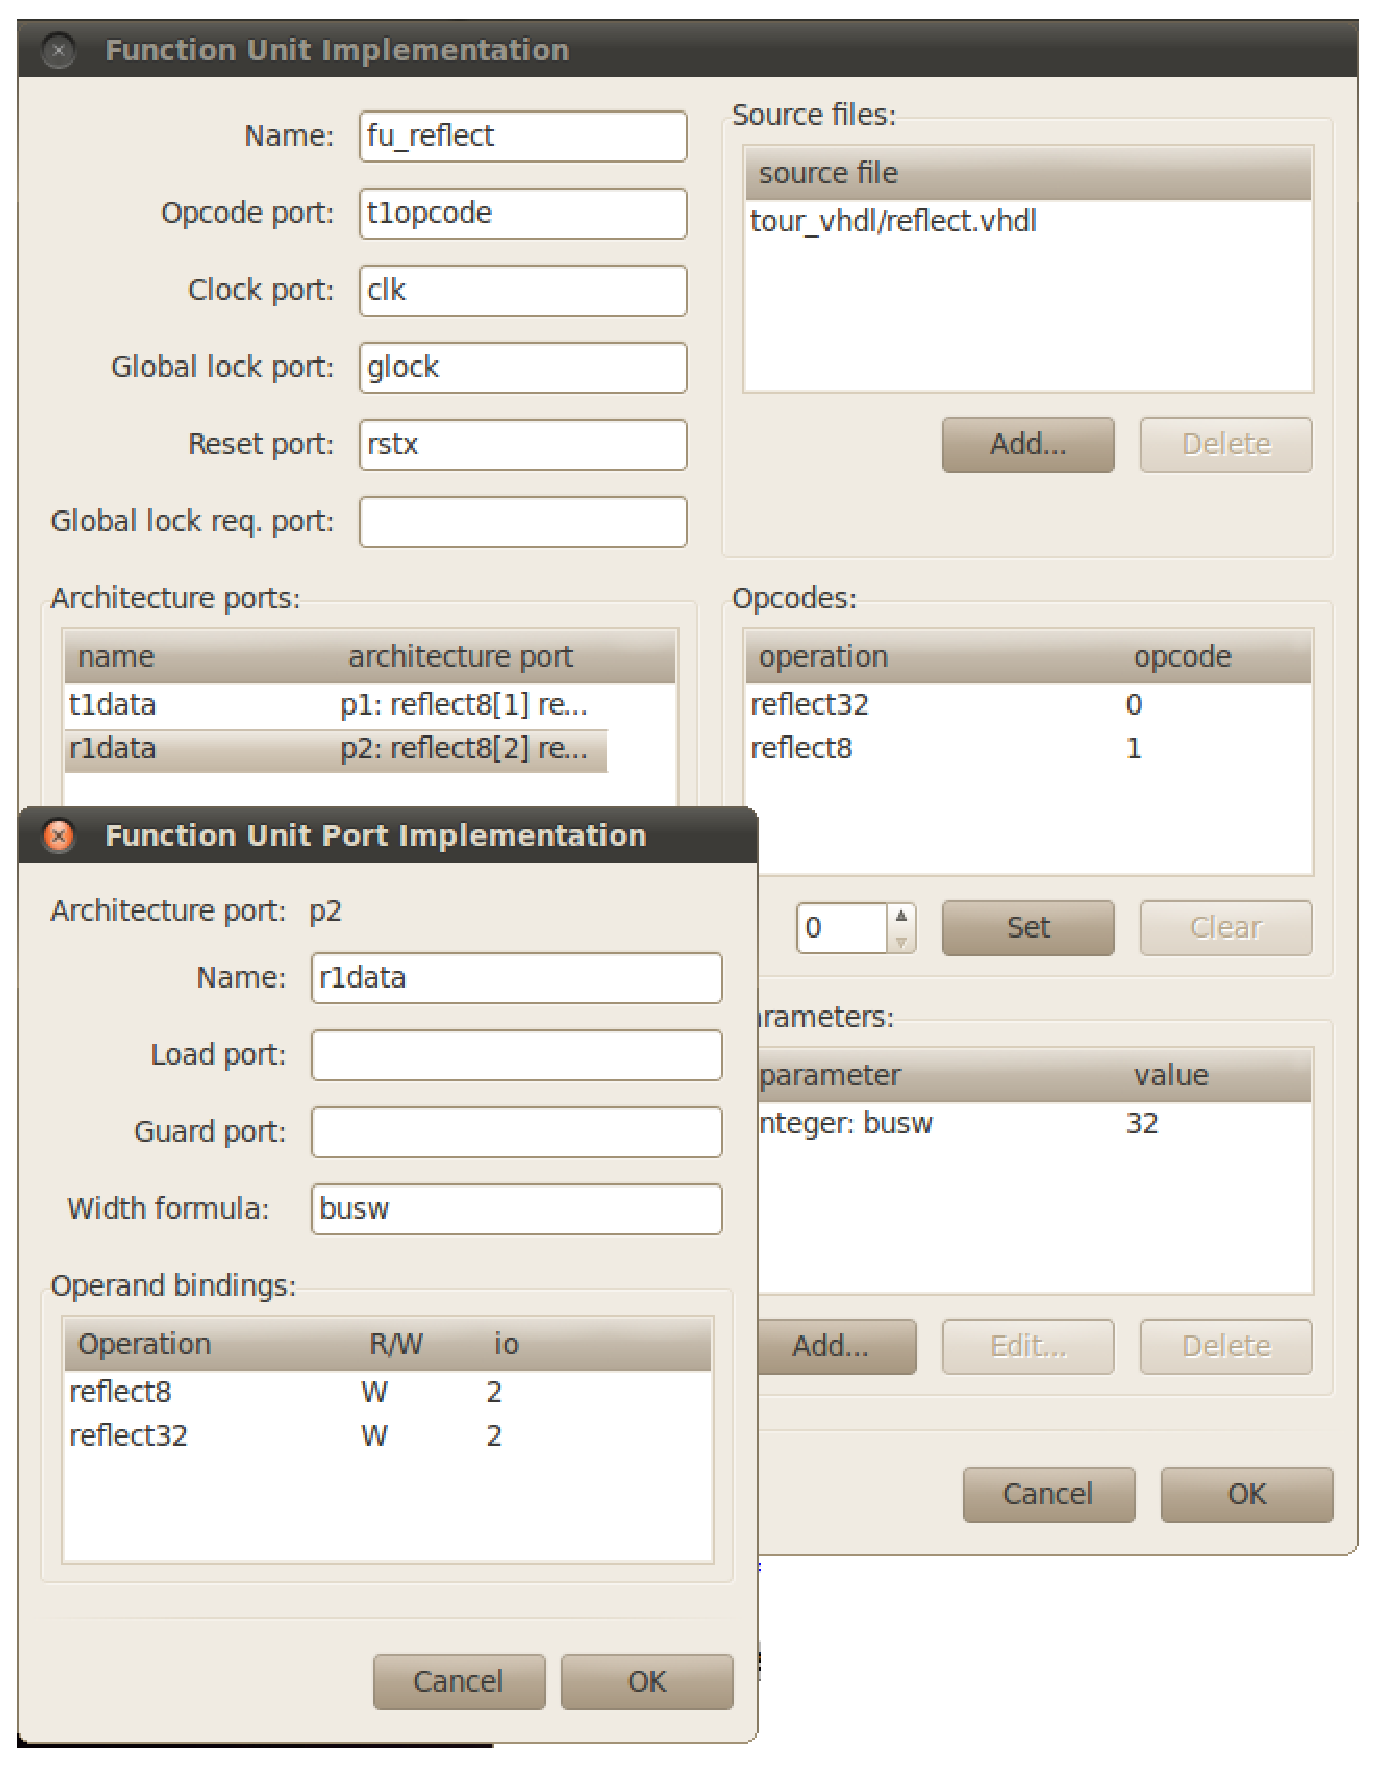
\includegraphics[width=0.8\textwidth]{eps/hdbeditor_scrshot}
  \caption{Adding the implementation of custom operations to HW database} 
  \label{fig:hdbed} \end{center}
\end{figure}

\item%
The HDB implementation dialog needs the following information from the VHDL:\\

\textbf{1. Name of the entity and the naming of the FU interface ports.}

Name the implemention after the top level entity: ``fu\_reflect''.

By examining the VHDL code you can easily spot the clock port (clk),
reset (rstx) and global lock port (glock). Operation code (opcode)
port is t1opcode. Write these into the appropriate text boxes. You do
not have to fill the Global lock req. port field because the function
unit does not stall, i.e. does not request a global lock to the
processor during its execution.

\textbf{2. Opcodes.}

Set the operation codes as they are in the top of the vhdl file. REFLECT32
has operation code ``0'' and REFLECT8 has operation code ``1''. 

The operation codes must be always numbered according to the alphabetical order of 
the OSAL operation names, starting at 0. For example, in this case REFLECT32 is 
earlier than REFLECT8 in the alphabetical order (i.e. 3 becomes before 8).

\textbf{3. Parameters.}

Parameters can be found from the VHDL generics. On top of the file there is one
parameter: busw. It tells the width of the transport bus and thus the maximum
width of input and output operands.

Thus, add parameter named busw, type it as integer and set the value to 32 in the
Parameter dialog.

\textbf{4. Architecture ports.}

These settings define the connection between the ports in the
architectural description of the FU and the VHDL implementation.
Each input data port in the FU is accompanied with a load port that
controls the updating of the FU input port registers.

Choose a port in the Architecture ports dialog and click edit.  Name
of the architecture port p1 is t1data (as in VHDL) and associated load
port is t1load.  Width formula is the parameter busw. No guard port is
needed in this case.

Name the output port (p2) to r1data and the width formula is now busw
because the output port writes to the bus.
The output port does not have a load port.

\textbf{5. Add VHDL source file.}

Add the VHDL source file into the Source code dialog. Notice that the HDL
files must be added in the compilation order (see section \ref{sec:hdbedit}).
But now we have only one source file so we can simply add it without
considering the compilation order (Add -> Browse -> tour\_vhdl/reflect.vhdl).

Now you are done with adding the FU implementation, see Fig.~\ref{fig:hdbed}. Click OK.

\end{enumerate}

\subsection{Generating the VHDL and memory images}
\label{ssec:tcetour_final_products}

In this step we generate the VHDL implementation of the processor, and the
bit image of the parallel program.

\paragraph{Select Function Unit Implementations}

% Then create an encoding for the instructions in the architecture:
% 
% \shellcmd{createbem custom.adf}
% 
% This should generate \file{custom.bem} which is a description on how
% instructions should be encoded in the architecture.
% 
% You can print the encoding info in a more human readable format with:
% 
% \shellcmd{viewbem custom.bem}
% 
% The program should print details on how each type of source/destination, etc.
% is encoded. You do not have to care about this, it is just for curiosity.
% Maybe the only important part in the printout is the length of the
% instruction word. In this case, even though the processor has only
% one move slot, the instruction word width is more than 40 bits. The size can
% be reduced with instruction compression and smaller immediate width, 
% which is skipped in the tutorial.

You can either use the given \file{custom\_operations.idf} included in the
tutorial files or select the implementations yourself. If you use the given
file replace \file{custom.idf} with \file{custom\_operations.idf} in the
following commands.

Next, we must select implementations for all components in the architecture.
Each architecture component can be implemented in multiple ways, so we must
choose one implementation for each component to be able to generate the
implementation for the processor.

This can be done in the ProDe tool:

\shellcmd{prode custom.adf}

Then we'll select implementations for the FUs which can be done in
\textit{Tools>Processor Implementation...}. Note that the selection window
is not currently very informative about the different implementations, so a
safe bet is to select an implementation with parametrizable width/size.

\begin{enumerate}
\item%
Selecting implementations for register files, immediate units and function
units can be done two different ways.

\begin{enumerate}
\item%
Manual selection - user chooses the implementations from HDB files.

\begin{enumerate}
\item%
Select implementation for RF: Click the RF name, 'Select Implementation',
find the TCE's default HDB file (PREFIX/share/tce/hdb/asic\_130nm\_1.5V.hdb) 
from your tce installation path and select an implementation for the RF from 
there.

\item%
Next select implementation for the boolean RF like above. But this time
select an implementation which is guarded i.e. select an implementation which
has word ``guarded\_0'' in its name.

\item%
Similarly, select implementations for the function units from TCE's default
HDB. Notice that it is vital that you choose the implementation for LSU from
the asic\_130nm\_1.5V.hdb. Then select implementation for the reflecter but
this time you have to use the \file{tour.hdb} created earlier to find the FU
we added that supports the REFLECT custom operations.
\end{enumerate}

\item%
Automatic selection - ProDe chooses the implementations from HDB files.

\begin{enumerate}
\item% 
Select implementations for register files and function units all at once: 
Click Auto Select Implementations, find the TCE's default HDB file from your 
TCE installation path (PREFIX/share/tce/hdb/asic\_130nm\_1.5V.hdb), make sure
'Register Files' and 'Function Units' checkboxes are checked and press 'Find'.
A dialog should appear saying 4 implementations were found; 2 for register
files and 2 for function units. Click 'Yes'. If the number of found
implementations was under 4 in your case, refer to the manual implementation 
selection above.

\item%
Browse to Function Units page if you were not on it already. You should see, 
that reflecter FU is still without implementation (because it is not defined 
in asic\_130nm\_1.5V.hdb). Select Auto Select Implementations again, find 
\file{tour.hdb} as the HDB file, and press 'Find'. 1 FU implementation should
be found (the reflecter), click 'Yes'. Now all your register files and 
function units should have implementations.
\end{enumerate}

\end{enumerate}

\item%
Next select the IC/Decoder generator plugin used to generate the
decoder in the control unit and interconnection network:
\textit{Browse... (installation\_path)/share/tce/icdecoder\_plugins/base/
DefaultICDecoderPlugin.so>OK}. This should be selected by default.

\item%
Enable bus tracing from the Implementation-dialog's IC / Decoder Plugin tab.
Set the bustrace plugin parameter to ``yes'' and the bustracestartingcycle to
``5''. The IC will now have a component which writes the bus value from every
cycle to a text file. Notice that this option cannot be used if the processor
is synthesized.

You do not have to care about the HDB file text box because we are not going 
to use cost estimation data.

\item%
Click ``Save IDF...''
\end{enumerate}



% TODO: Add this when unit tester is stable enough
%\paragraph{Unit testing}
%
%Now that we have selected the implementations for FUs we can run unit tests on
%them. TTA unit tester checks that the operation simulation behaviour model and
%RTL implementation of an FU are equal. Testing is done with command:
%
%\shellcmd{ttaunittester -a custom.adf custom.idf}
%
%Test will output that it cannot test one FU implementation because it has
%external ports. This is not a failure. If some implementation is not equal
%to operation definitions


\paragraph{Generate the VHDL for the processor using Processor Generator
(ProGe).}

You can start processor generation from ProDe's implementation selection dialog:
Click ``Generate Processor''. For Binary Encoding Map: Select the
``Generate new'', see Fig.~\ref{fig:proge} 

In the target directory click ``Browse'' and create a new
directory \file{proge-output} and select it. Then click OK to create the
processor.

\begin{figure}
  \begin{center} 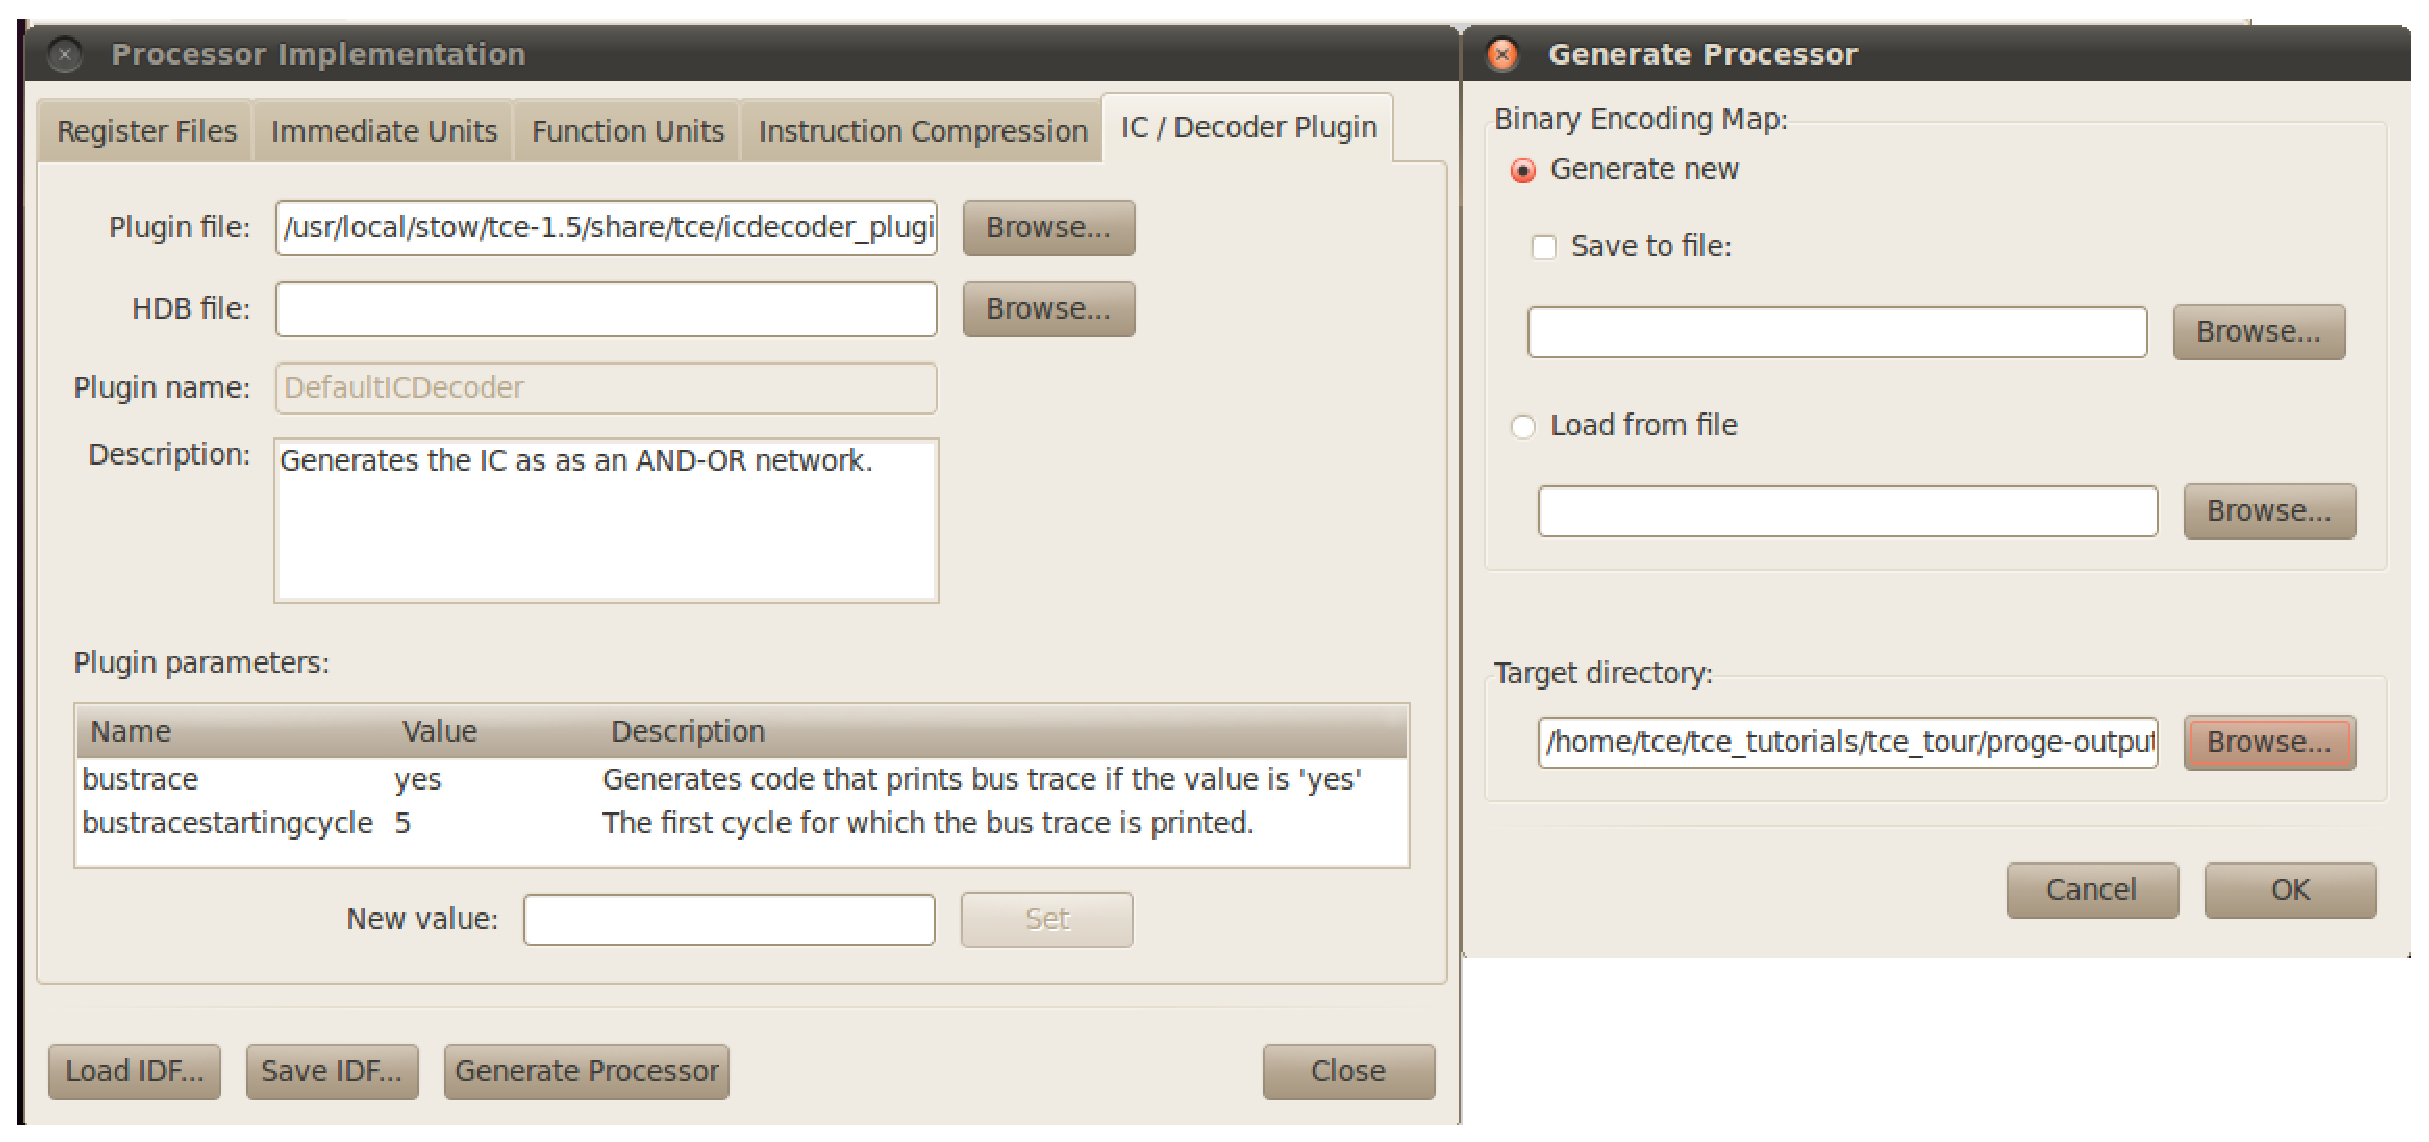
\includegraphics[width=0.8\textwidth]{eps/proge_scrshot}
  \caption{Generating TTA VHDL with ProGe} 
  \label{fig:proge} \end{center}
\end{figure}


Or alternatively execute ProGe from command line:

\shellcmd{generateprocessor -t -i custom.idf -o proge-output
custom.adf}

Flag $-t$ generates a testbench, $-i$ defines the implementation file,
and $-o$ the output directory.  Now directory \file{proge-output}
includes the VHDL implementation of the designed processor except for
the instruction memory width package which will be created by Program
Image Generator. You can take a look what the directory includes, how
the RF and FU implementations are collected up under
\file{vhdl} subdir and the interconnection network has been generated to
connect the units (the \file{gcu\_ic} subdir). The \file{tb} subdir
contains testbench files for the processor core. Moreover, there are 4
shell scripts for compiling and simulating the VHDL codes in Modelsim
and GHDL.

\paragraph{Generate instruction memory bit image using Program Image Generator.}

Finally, to get our shiny new processor some bits to chew on,
we use generatebits to create instruction memory and data memory images:

\shellcmd{generatebits -d -w 4 -p crc\_with\_custom\_op.tpef -x proge-output custom.adf} 

Flag $-d$ creates data images, $-w 4$ set data memory width 4 MAUs
(Minimum Addressable Units, bytes in this case), $-p$ defines the
program, $-x$ defines the HDL directory, and adf is given without a
flag.

Now the file \file{crc\_with\_custom\_op.img} includes the instruction memory
image in ``ascii 0/1'' format. Each line in that file represents a single
instruction. Thus, you can get the count of instructions by counting the
lines in that file:

\begin{verbatim}
 wc -l crc_with_custom_op.img
\end{verbatim}

%% NOTE: bem is not generated in this version of tutorial
%By multiplying the count with the instruction width we found earlier you
%can get the required size of instruction memory for the program.

Accordingly, the file \file{crc\_with\_custom\_op\_data.img} contains the data
memory image of the processor. Program Image Generator also created file
\file{proge-output/vhdl/tta0\_imem\_mau\_pkg.vhdl} which contains the 
width of the instruction memory (each designed TTA can have a different 
instruction width). The \_imem\_mau\_pkg.vhdl file is appended with the top
level entity name, which in this case is ``tta0''.

\paragraph{Simulation and verification}

If you have GHDL installed you can now simulate the processor VHDL. First
cd to proge-output directory:

\shellcmd{cd proge-output}

Then compile and simulate the testbench:

\shellcmd{./ghdl\_compile.sh}

\shellcmd{./ghdl\_simulate.sh}

Compilation gives a couple of warnings from Synopsys' std\_arith
package but that should do no harm.  Simulation will take some time as
the bus trace writing is enabled. If you did not change the memory
widths in Prode (Section~\ref{ssec:start_point} ), the simulation will crash and print
``Killed''. There will be many warnings at $0 ns$ due uninitialized
signals but you can ignore them. 

Aftern simulation, you should see a message
\shellcmd{./testbench:info: simulation stopped by --stop-time}
The simulation produces file ``bus.dump'' which looks like this:
\begin{verbatim}
           0 |            0 | 
           1 |            4 | 
           2 |        32760 | 
           3 |           24 | 
           ...
\end{verbatim}


As the testbench is ran for constant amount of cycles we
need to get the relevant part out of the bus dump for
verification. This can be done with command:

\shellcmd{head -n <number of cycles> bus.dump > sim.dump}

where the <number of cycles> is the number of cycles in the previous
ttasim execution (same as line ocunt in
crc\_with\_custom\_op.tpef.bustrace). Then compare the trace dumps
from the VHDL simulation and the architecture simulation:

\shellcmd{diff -u sim.dump ../crc\_with\_custom\_op.tpef.bustrace}

If the command does not print anything the dumps were equal and GHDL
simulation matches the ttasim. Now you have succesfully added a custom
operation, verified it, and gained notably performance increase. Well
done!


\subsection{Further acceleration by adding custom operation to large TTA}
\label{ssec:large_custom}

As a final step, let us add the custom operation to the large TTA.

\shellcmd{cp large.adf large\_custom.adf}

\shellcmd{prode large\_custom.adf}

%% Copy-paste between ProDe windows might be a bit fragile..
%
%Open also custom.adf. Copy-paste the REFLECTER unit from it to
%large\_custom.adf. Fully connect the IC, as in
%Fig.\ref{fig:prode_largecustom} and save.

Add the reflecter FU from the tour.hdb like done earlier. Fully
connect the IC, as in Fig.\ref{fig:prode_largecustom} and save.

\begin{figure}
  \begin{center}
    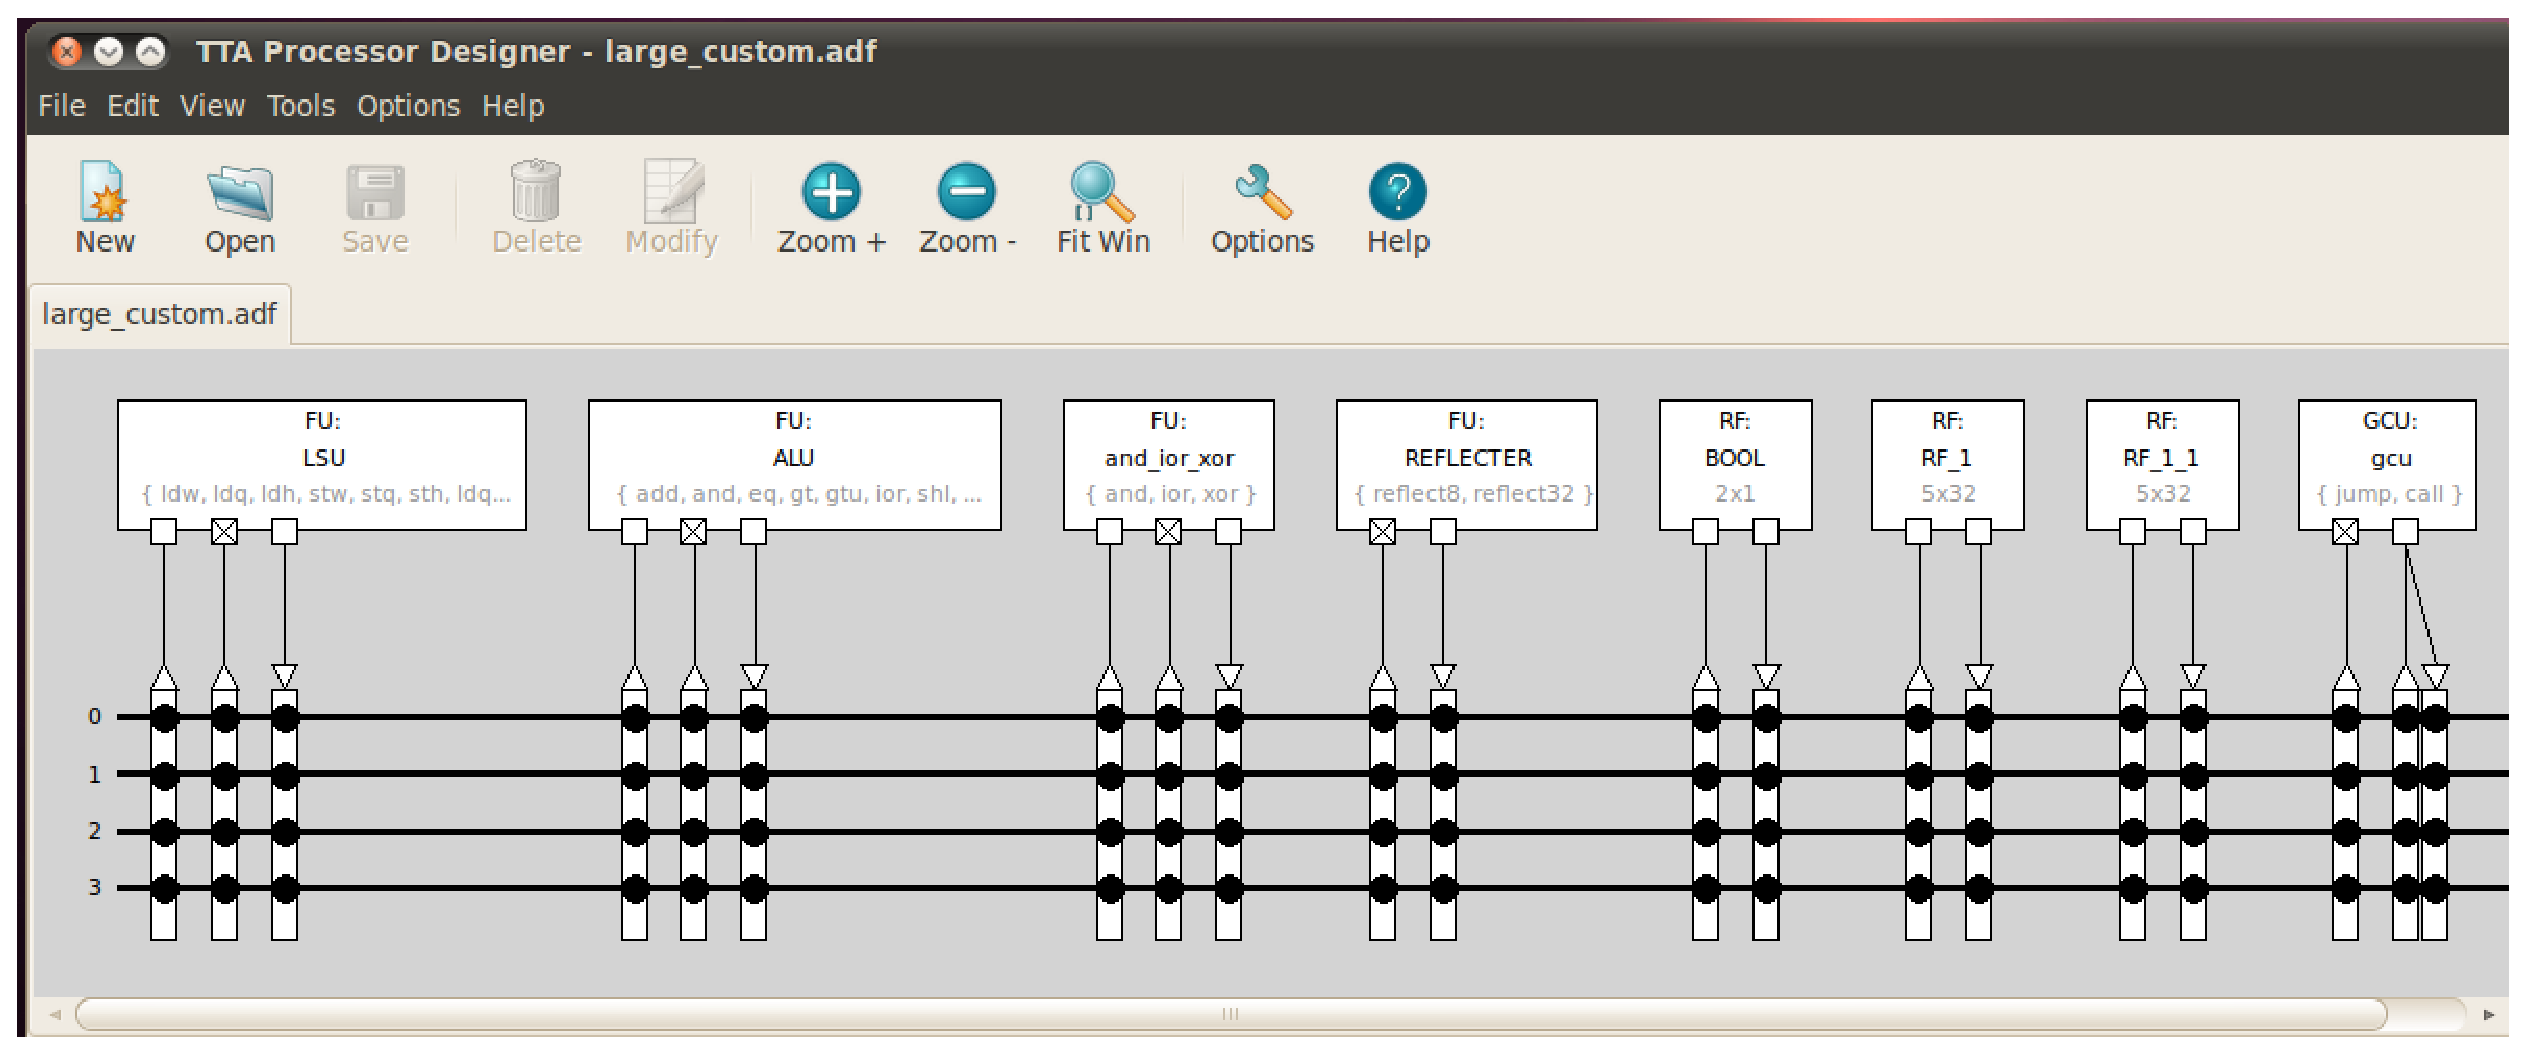
\includegraphics[width=10cm]{eps/prode_largecustom}
    \caption{Processor Designer (prode) with large\_custom.adf}
    \label{fig:prode_largecustom}
  \end{center}
\end{figure}


\shellcmd{tcecc -O3 -a large\_custom.adf -o crc\_with\_custom\_op.tpef -k result crc\_with\_custom\_op.c main.c}

\shellcmd{ttasim -a large\_custom.adf -p crc\_with\_custom\_op.tpef}

\shellcmd{info proc cycles}

Voila! Now you have a lightning fast TTA. % 100 cycles

\subsection{Final Words}

This tutorial is now finished. Now you should know how to customize
the processor architecture by adding resources and custom operations,
as well as generate the processor implementation and its instruction
memory bit image.

This tutorial used a ``minimalistic'' processor architecture as our
starting point. The machine had only 1 transport bus and 5 registers
so it could not fully exploit the parallel capabilities of TTA.  Then
we increased resources in the processor and the cycle count dropped to
half. Adding 2 simple custom operations to the starting point
architecture gives a similar speedup and in large machine the speedup
in cyclecount is about $50x$.

\section{From C to VHDL as Quickly as Possible}
\label{section:fromCtoVHDL}
% NOTE: when updating this update also c2vhdl systemtest if needed.
% TODO: Also add compilation and simulation of VHDL code using GHDL
 
This tutorial introduces a fast way to generate a processor VHDL model
from C source code using the Design Space Explorer.
 
If you haven't already downloaded the tutorial file package, you can get it 
from:\\
\url{http://tce.cs.tut.fi/tutorial_files/tce_tutorials.tar.gz} \\
Unpack it to a working directory and then cd to tce\_tutorials/c2vhdl/

A script named c2vhdl should generate all the needed files from the C source
code. The script is a bash script using various TCE command line tools, and
can be inspected for detailed instructions to generate the VHDL and other
files manually.

\shellcmd{c2vhdl application1/complex\_multiply.c}

Now directory called ``proge-output'' should include the VHDL implementation
of the processor.
The current working directory should also contain the instruction memory bit
image file and the instruction encoding (bem) file along with the processor
architecture definition and implementation definition files.

Passing "-e" as the first parameter to c2vhdl script tells it to print
estimation data, like area and energy requirements for the processor it
generates.

Tutorial is now finished and you can simulate the generated VHDL
implementation of the processor with a VHDL simulator and synthesize it.


%%%%%%%%%%%%%%%%%%%%%%%%%%%%%%%%%%%%%%%%%%%%%%%%%%%%
% THESE ARE TODO's
%%%%%%%%%%%%%%%%%%%%%%%%%%%%%%%%%%%%%%%%%%%%%%%%%%%%
%
%\section{Manual Exploration}
%\label{section:manualExpl}
% Modify the arch manually until it meets the requirements

%\section{Automated Design Space Exploration}
%\label{section:automatedExploration}
% Add requirements and sequential programs, 
% Click, click, *wait a couple of weeks*, done! ;-)


\section{Hello TTA World!}

What would a tutorial be without the traditional ``Hello World!''
example? Interestingly enough, printing out ``Hello World'' in a
standalone (operating system free) platform like the TTA of TCE is not 
totally straightforward. That is the reason this tutorial is not the first 
one in this tutorial chapter.

The first question is: where should I print the string? Naturally 
it is easy to answer that question while working with the simulator: to
the simulator console, of course. However, when implementing the final
hardware of the TTA, the output is platform dependent. It can be a
debugging interface, serial port output, etc.

In order to make printing data easier from TTAs designed
with TCE, we have included an operation called STDOUT in the ``base operation 
set'' that is installed with the TCE. The simulation behavior of the 
operation reads its input, expects it to be a 8bit char and writes the char
verbatim to the simulator host's standard output. Of course, in case the 
designer wants to use the operation in his final system he must provide the 
platform specific implementation for the function unit (FU) implementing the 
operation, or just remove the FU after the design is fully debugged and
verified.

The default implementation of \textit{printf()} in TCE uses the STDOUT
operation to print out data. Therefore, implementing a ``Hello World''
application with TCE is as simple as adding an FU that implements
the STDOUT to the processor design and then calling \textit{printf()} in
the simulated program. The simulator should print out the greeting
as expected.

Here is a simple C code (hello.c) that prints the magic string:

\begin{verbatim}
#include <stdio.h>

int main() {
    printf("Hello TTA World!");
    return 0;
}
\end{verbatim}

Next, compile it to an architecture that implements the
STDOUT. TCE ships with a minimal architecture that also includes
the STDOUT function unit, which you can use:

\begin{verbatim}
cp $(tce-config --prefix)/share/tce/data/mach/minimal_with_stdout.adf .
tcecc --swfp -O0 hello.c -a minimal_with_stdout.adf -o hello.tpef
\end{verbatim}

%$ this dollar sign ``closes'' the equation, so syntax highlight works correctly

It should compile without errors. Beware: the compilation can take
a while on a slower machine. This is because \textit{printf()} 
is actually quite a large function and the compiler is not yet optimized for 
speed.

Finally, simulate the program to get the greeting:

\begin{verbatim}
ttasim -a minimal_with_stdout.adf -p hello.tpef --no-debugmode
Hello TTA World!
\end{verbatim}

That's it. Happy debugging!

\section{Streaming I/O}
\label{section:streamIO}

Because TTA/TCE is an environment without operating system, there is also
no file system available for implementing file-based I/O. Therefore, one
popular way to get input and output to/from the TTA is using shared memory
for communicating the data. For stream processing type of applications,
one can also use an I/O function unit that implements the required 
operations for streaming.

TCE ships with example operations for implementing stream type input/output. 
These operations can be used to read and write samples from streams in the
designed TTA processor. The basic interface of the operations allows reading and 
writing samples from the streams and querying the status of an input or output stream 
(buffer full/empty, etc.). The status operations are provided to
allow the software running in the TTA to do something useful while the
buffer is empty or full, for example switch to another thread. Otherwise,
in case one tries to read/write a sample from/to a stream whose buffer is 
empty/full, the TTA is locked and the cycles until the situation resolves
are wasted.

The example streaming operations in the base operation set are 
called STREAM\_IN, STREAM\_OUT, STREAM\_IN\_STATUS, and STREAM\_OUT\_STATUS.
These operations have a simulation behavior definition which simulates the
stream I/O by reading/writing from/to files stored in the file system of 
the simulator host.

Here is an example C code that implements streaming I/O with the operations:

\begin{verbatim}
#include "tceops.h"

int main()
{
    char byte;
    int status;

    while (1)
    {
        _TCE_STREAM_IN_STATUS(0, status);

        if (status == 0)
            break;

        _TCE_STREAM_IN(0, byte);
        _TCE_STREAM_OUT(byte);
    }

    return 0;
}
\end{verbatim}

This code uses the TCE operation invocation macros from \textit{tceops.h}
to read bytes from the input stream and write the same bytes to the
output stream until there is no more data left. This situation is indicated
with the status code 0 queried with the STREAM\_IN\_STATUS operation. The
value means the stream buffer is empty, which means the file simulating the
input buffer has reached the end of file.

You can test the code by creating a file \textit{<FU\_NAME>.in} with some test
data, compiling the code and simulating it. The code should create a copy of
that file to the stream output file \textit{<FU\_NAME>.out}. These files
should reside in the directory where the simulator is started. You can get
the FU\_NAME from the streaming function units in the adf file.

\subsection{Streaming I/O function units}
VHDL implementations and HDB entries for streaming I/O have been included 
in TCE since version 1.4. The \textit{stream.hdb} -file in the TCE installation
directory contains one function unit with STREAM\_IN and
STREAM\_IN\_STATUS -operations, and another FU contains the STREAM\_OUT and STREAM\_OUT\_
STATUS
-operations. These FUs can directly be instantiated in ProDe and synthesized
on an FPGA along with the rest of the processor.

When these function units are instantiated in ProDe, they are realized with
specific operation latencies. STREAM\_IN and STREAM\_OUT
take 3 clock cycles, and STREAM\_IN\_STATUS and STREAM\_OUT
\_STATUS execute in 1 clock cycle.

The Stream In -FU has three external ports. \textit{ext\_data} is 8 bits wide
and is used to communicate the data byte from the external stream source to the 
TTA FU. When the TTA application program invokes the STREAM\_IN -operation, the
\textit{ext\_data} signal is sampled by the FU and the Stream In -FU automatically sends
an acknowledge-signal back to the stream source through the \textit{ext\_ack}
port of the FU. The external stream source is supposed to provide the next stream
data value to \textit{ext\_data} upon noticing a rising edge in \textit{ext\_ack}.
The three cycle latency of the operation allows some time for this to happen. Finally,
the TTA application program can query the availability of stream data by invoking
the STREAM\_IN\_STATUS -operation. This command reads the value of the \textit{ext\_status}
port of the Stream In FU and the external stream device is expected to keep the signal
high in this port when there is still data available, and low when the stream 
device has run out of data. The application program sees the status as a numerical 
value '1' or '0'.

The Stream Out -FU works in a similar fashion. The \textit{ext\_data} port is now 
an output and provides the data to the external stream sink. The external stream
sink is expected to sample the value of \textit{ext\_data} when \textit{ext\_dv}
(data valid) is high. \textit{ext\_dv} is automatically operated by the FU when
the application program invokes the operation STREAM\_OUT. STREAM\_OUT has also
a latency of 3 clock cycles to allow the external stream sink to take care of the
data sample. Invoking the STREAM\_OUT\_STATUS operation samples the signal in
the \textit{ext\_status} -port, which the external stream sink is expected to keep
high if there is still space in the stream sink. When the stream sink is full, the
signal in the \textit{ext\_status} -port must be pulled low by the stream sink.

Having several distinct stream sources or sinks must at the moment be realized
by manually copying the FUs along with their HDB and VHDL parts. The operations
must have distinct names so that the compiler is explicitly instructed to read
from a specific source or write to a specific sink.

\section{Implementing Programs in Parallel Assembly Code}
\label{section:parallelAssemblyCoding}
% TODO: add example of implementing a sort RISC assembly code as
% a parallel TTA program. How to compile it (refer to assembler section) and
% how to simulate and estimate it, etc.

This tutorial will introduce you to TTA assembly programming. It is
recommended that you go through this tutorial because it will certainly
familiarize you with TTA architecture and how TTA works.

\subsection{Preparations}

For the tutorial you need to download file package from
\url{http://tce.cs.tut.fi/tutorial_files/tce_tutorials.tar.gz} and unpack it
to a working directory. Then cd to parallel\_assembly-directory.

The first thing to do is to compile the custom operation set called cos16 shipped
within the parallel\_assembly-directory. The easiest way to do this is:

\shellcmd{buildopset cos16}

This should create a file named \file{cos16.opb} in the directory.

\subsection{Introduction to DCT}

Now you will be introduced to TCE assembler language and assembler usage.
Your task is to write TCE assembly code for 2-Dimensional 8 times 8 point 
Discrete Cosine Transform (DCT\_8x8).
First take a look at the C code of DCT\_8x8
\file{dct\_8x8\_16\_bit\_with\_sfus.c}.  
The code is written to support fixed point datatype with sign plus 15 fragment
bits, which means coverage from $-1\ to\ 1-2^{15}$. The fixed point
multiplier, function \textit{mul\_16\_fix}, and fixed point adder, function
\textit{add\_16\_fix},  used in the code scale inputs automatically to prevent
overflow. Function \textit{cos16} takes $x(2i+1)$ as input and returns
the corresponding cosine value $cos\left(\frac{x(2i+1)\pi}{16}\right)$. The code calculates
following equations:

\begin{equation}
F(x) = \frac{C(x)}{2}\sum_{i = 0}^7 \left[f(i)cos\left(\frac{x
\left(2i+1\right)\pi}{16}\right)\right] \nonumber
\end{equation}
\begin{equation}
F(y) = \frac{C(y)}{2}\sum_{i = 0}^7 \left[f(i)cos\left(\frac{y
\left(2i+1\right)\pi}{16}\right)\right] \nonumber
\end{equation}

\begin{equation}
C(i) = 
\left\{
\begin{array}{c c}
\frac{2}{\sqrt2} &,  i = 0 \\
1 &,  else 
\end{array} \right . . \nonumber
\end{equation}

\begin{equation}
F(x,y) = F(x)F(y) \nonumber
\end{equation}

\subsection{Introduction to TCE assembly}

First take a look at assembly example in file \file{example.tceasm}
to get familiar with syntax. More help can be found from
section \ref{section:TCEAsm}

Compilation of the example code is done by command:

\shellcmd{tceasm \ -o \ example.tpef \ dct\_8x8\_16\_bit\_with\_sfus.adf \
example.tceasm}

The assembler will give some warnings saying that ``Source is
wider than destination.'' but these can be ignored.

The compiled tceasm code can be simulated with TCE
simulator, ttasim or proxim(GUI).

\shellcmd{ttasim -a \ dct\_8x8\_16\_bit\_with\_sfus.adf -p example.tpef} , or

\shellcmd{proxim \ dct\_8x8\_16\_bit\_with\_sfus.adf example.tpef}

It is recommended to use proxim because it is more illustrating to track the
execution with it. Especially if you open the Machine Window (View -> Machine
Window) and step through the program.

Check the result of example code with command (you can also write this in
proxim's command line at the bottom of the main window):

\shellcmd{x /a IODATA /n 1 /u b 2}. 

the output of x should be 0x40.

\subsection{Implementing DCT on TCE assembly}

Next try to write assembly code which does the same functionality as the
C code. The assembly code must be functional with the given machine
\file{dct\_8x8\_16\_bit\_with\_sfus.adf}. Take a look at the processor by
using prode:

\shellcmd{prode dct\_8x8\_16\_bit\_with\_sfus.adf \&}

The processor's specifications are the following:

\textbf{Supported operations} \\
Operations supported by the machine are: \textit{mul}, \textit{mul\_16\_fix},
\textit{add}, \textit{add\_16\_fix}, \textit{ldq}, \textit{ldw}, \textit{stq},
\textit{stw}, \textit{shr}, \textit{shl}, \textit{eq}, \textit{gt},
\textit{gtu}, \textit{jump}, \textit{cos16} and \textit{immediate transport}.

When you program using TTA assembly you need to take into account 
operation latencies. The \textit{jump} latency is four clock cycles and load
latencies (\textit{ldq} and \textit{ldw}) are three cycles. Latency for
multiplications (\textit{mul} and \textit{mul\_16\_fix}) are two clock cycles.

\textbf{Address spaces} \\
The machine has two separate address spaces, one for data and another for
instructions. The data memory is 16-bit containing 128 memory slots and the
MAU of data memory is 16-bits. The instruction memory has 1024 memory slots
which means that the maximum number of instructions of 1024.

\textbf{Register files} \\
The machine contains 4 register files, each of which have 4 16-bit registers,
leading to total of 16 16-bit registers.  The first register file
has 2 read ports.

\textbf{Transport buses} \\
The machine has 3 16-bit buses, which means maximum of 3 concurrent
transports. Each bus can contain a 8-bit short immediate.

\textbf{Immediates} \\
Because the transport buses can only contain 8-bit short immediates you must
use the immediate unit if you want to use longer immediates. The immediate unit
can hold a 16-bit immediate. There is an example of immediate unit usage in
file \file{immediate\_example.tceasm}. Basically you need to transfer the value to the
immediate register. The value of immediate register can be read on the next
cycle.

The initial input data is written to memory locations 0-63 in the file
\file{assembler\_tutorial.tceasm}. Write your assembly code in that file.

\subsubsection{Verifying the assembly program}

The reference output is given in \file{reference\_output}. You need to
compare your assembly program's simulation result to the reference
output. Comparision can be done by first dumping the memory contents in the
TCE simulator with following command:

\shellcmd{x /a IODATA /n 64 /u b 0}

The command assumes that output data is stored to memory locations 0-63.

The easiest way to dump the memory into a text file is to execute ttasim with
the following command:

\shellcmd{ttasim -a dct\_8x8\_16\_bit\_with\_sfus.adf -p
assembler\_tutorial.tpef < input\_command.txt > dump.txt}

After this you should use sed to divide the memory dump into separete lines
to help comparison between your output and the reference output. Use the
following command to do this (there is an empty space between the
first two slashes of the sed expression):

\shellcmd{cat dump.txt | sed 's/ /$\backslash$n/g' > output.txt}

And then compare the result with reference:

\shellcmd{diff -u output.txt reference\_output}

When the TCE simulator memory dump is the same as the reference output your
assembly code works and you have completed this tutorial. Of
cource you might wish to improve your assembly code to minimize cycle
count or/and instruction count.

You should also compile the C program and run it because it gives more
detailed information which can be used as reference data if you need to debug
your assembly code.

To compile the C code, enter:

\shellcmd{gcc -o c\_version dct\_8x8\_16\_bit\_with\_sfus.c}

If you want the program to print its output to a text file, you can use the
following command:

\shellcmd{./c-version > output.txt}


To get some idea of the performance possibilities of the machine,
one assembly code has 52 instructions and it runs the DCT8x8 in
3298 cycles.

\section{Using multiple memories from C code}

TCE supports accessing multiple address spaces from C code via the
\_\_attribute\_\_((address\_space(N)) extension. The numerical id from
the attribute is used to connect the memory reference to the ADF 
address space using the XML element \textbf{numerical-id}. There can be
one or more numerical ids mapped to a single ADF address space.

The following is from an ADF with three separate data address spaces with
numerical ids 0, 1, and 2. The numerical id 0 is reserved for the default 
data address space which stores the stack, heap and the global constant 
data.

\begin{verbatim}
   <address-space name="data">
    <width>8</width>
    <min-address>0</min-address>
    <max-address>16777215</max-address>
    <numerical-id>0</numerical-id>
  </address-space>

  <address-space name="data1">
    <width>8</width>
    <min-address>0</min-address>
    <max-address>65535</max-address>
    <numerical-id>1</numerical-id>
  </address-space>

  <address-space name="data2">
    <width>8</width>
    <min-address>0</min-address>
    <max-address>16383</max-address>
    <numerical-id>2</numerical-id>
  </address-space>
\end{verbatim}

The address spaces can be referred to from the C program with code
like this:

\begin{verbatim}
#include <stdio.h>

#define ASIZE 4

volatile int space0[ASIZE] __attribute__((address_space(0)));
volatile int space0_1[ASIZE] __attribute__((address_space(0)));
volatile int space1[ASIZE] __attribute__((address_space(1)));
volatile int space1_1[ASIZE] __attribute__((address_space(1)));
volatile int space2[ASIZE] __attribute__((address_space(2)));
volatile int space2_1[ASIZE] __attribute__((address_space(2)));

int main() {
    int i = 0;

    /* The start addresses of the tables should overlap as
       they are allocated in different address spaces. */
    iprintf("space0@%x space0_1@%x space1@%x space1_1@%x space2@%x space2_1@%x\n",
            (unsigned)space0, (unsigned)space0_1, (unsigned)space1, (unsigned)space1_1,
            (unsigned)space2, (unsigned)space2_1);

    return 0;
}
\end{verbatim}

The effect of having multiple disjoint address spaces is visible when 
simulating the code as the arrays allocated to the different memories share 
the same addresses but different storage:

\begin{verbatim}
space0@a84 space0_1@a94 space1@4 space1_1@14 space2@4 space2_1@14
\end{verbatim}

The space0 array is stored in the default address space. In the beginning
of the default address space there is usually some global data for 
some C library functions
such as the iprintf or the emulation library, thus ending up with the
start address of 0xa84 for the array0. For the extra address spaces
1 and 2, the arrays start from 4 which is the first valid storage address in
those address spaces. Storing data to address 0 is not done to avoid 
problems with NULL pointers pointing to valid data (in this case space1 and
space2 would have been stored at address 0 = NULL).

When using custom operation calls to manually execute operations that access
memory on processors that have multiple data address spaces,
it should be done using \_TCEAS\_OPERATIONNAME macro instead of using
\_TCE\_OPERATIONNAME macro. See section~\ref{sec:tceccCustOp}
 for more information about these custom operation call macros.

\section{Running TTA on FPGA}
\label{sec:fpgatutorial}

This tutorial illustrates how you can run your TTA designs on a FPGA board.
Tutorial consists of two simple example sections and a more general case
description section.

Download the tutorial file package from:

\url{http://tce.cs.tut.fi/tutorial_files/tce_tutorials.tar.gz}\\

Unpack it to a working directory and cd to tce\_tutorials/fpga\_tutorial

\subsection{Simplest example: No data memory}
\subsubsection{Introduction}
This is the most FPGA board independent TTA tutorial one can make. The
application is a simple led blinker which has been implemented using register
optimized handwritten TTA assembly. In other words the application
doesn't need a load store unit so there is no need to provide data memory. In
addition the instruction memory will be implemented as a logic array.

\subsubsection{Application}
The application performs a 8 leds wide sweep in an endless loop. Sweep 
illuminates one led at a time and starts again from first led after reaching
the last led. There is also a delay between the iterations so that the sweep
can be seen with human eye.

As stated in the introduction the application is coded in assembly. If you went
through the assembly tutorial the code is probably easy to understand. The code
is in file \file{blink.tceasm}. The same application is also written in C code
in file \file{blink.c}.

\subsubsection{Create TTA processor core and instruction image}
The architecture we're using for this tutorial is \file{tutorial1.adf}. Open it
in ProDe to take a look at it:

\shellcmd{prode tutorial1.adf}

As you can see it is a simple one bus architecture without a LSU. There are
also 2 ``new'' function units: rtimer and leds. Rtimer is a simple tick
counter which provides real time clock or countdown timer operations. Leds is
function unit that can write '0' or '1' to FPGA output port. If those ports
are connected to leds the FU can control them.

Leds FU requires a new operation definition and the operation is defined in
\file{led.opp} and \file{led.cc}. You need to build this operation defintion:

\shellcmd{buildopset led}

Now you can compile the assembly code:

\shellcmd{tceasm -o asm.tpef tutorial1.adf blink.tceasm}

If you wish you can simulate the program with proxim and see how it works but
the program runs in endless loop and most of the time it stays in the
``sleep'' loop.

Now you need to select implementations for the function units. This can be
done in ProDe. See TCE tour section \ref{ssec:tcetour_final_products} for more
information. Implementations for leds and rtimer are found from the fpga.hdb
shipped with the tutorial files. Notice that there are 2 implementations for
the rtimer. ID 3 is for 50 MHz clock frequency and ID 4 for 100 MHz. All other
FUs are found from the default hdb.

Save the implementation configuration to \file{tutorial1.idf}.
% After you have generated \file{tutorial1.idf} generate the binary encoding for
% the arhitecture:

% \shellcmd{createbem tutorial1.adf}

Next step is to generate the VHDL implementation of the processor:

% -b tutorial1.bem

\shellcmd{generateprocessor -i tutorial1.idf -o asm\_vhdl/proge-output tutorial1.adf}

Then create the proram image:

% -b tutorial1.bem

\shellcmd{generatebits -f vhdl -p asm.tpef -x asm\_vhdl/proge-output tutorial1.adf}

Notice that the instruction image format is ``vhdl'' and we request
generatebits to not create data image at all. Now, move the generated 
\file{asm\_imem\_pkg.vhdl} to the asm\_vhdl directory and cd there.

\shellcmd{mv asm\_imem\_pkg.vhdl asm\_vhdl/}

\shellcmd{cd asm\_vhdl}

\subsubsection{Final steps to FPGA}
We have successfully created the processor core and instruction memory image.
Now we need an instruction memory component that can use the generated image.
Luckily you don't have to create it as it is shipped with the tutorial files.
The component is in file \file{inst\_mem\_logic.vhd} in asm\_vhdl directory
and it can use the generated \file{asm\_imem\_pkg.vhdl} without any
modifications.

Next step is to connect TTA toplevel core to the memory component and connect
the global signals out from that component. This has also been done for you in
file \file{tutorial\_processor1.vhdl}. If you are curious how this is done
open the file with your preferred text editor. All the signals coming out of
this component are later connected to FPGA pins.

Now you need to open your FPGA tool vendor's FPGA design/synthesis program and
create a new project for your target FPGA. Add the three files in 
asm\_vhdl-directory (toplevel file \file{tutorial\_processor1.vhdl}, 
\file{inst\_mem\_logic.vhd} and \file{asm\_imem\_pkg.vhdl}) and all the
files in proge-output/gcu\_ic/ and proge-output/vhdl directories to the
project. The toplevel entity name is 'tutorial\_processor1'.

Then connect the toplevel signals to appropriate FPGA pins. The pins are most
probably described in the FPGA board's user manual. Signal 'clk' is obviously
connected to the pin that provides clock signal. Signal 'rstx' is the reset
signal of the system and it is active low. Connect it to a switch or
pushbutton that provides '1' when not pressed. Signal bus 'leds' is 8 bits
wide and every bit of the bus should be connected to an individual led. Don't
worry if your board doesn't have 8 user controllable leds, you can leave some
of them unconnected. In that case all of the leds are off some of the time.

Compile and synthesize your design with the FPGA tools, program your FPGA and
behold the light show!

\subsection{Second example: Adding data memory}

In this tutorial we will implement the same kind of system as above but this
time we include data memory and use C coded application. Application has
the same functionality but the algorithm is a bit different. This time we read the
led pattern from a look up table and to also test store operation the pattern
is stored back to the look up table. Take a look at file \file{blink\_mem.c}
to see how the timer and led operations are used in C code.

\subsubsection{Create TTA processor core and binary images}

The architecture for this tutorial is \file{tutorial2.adf}. This architecture
is the same as \file{tutorial1.adf} with the exception that now it has a load
store unit to interface it with data memory.

You need to compile the operation behaviour for the led function unit if you
already haven't done it:

\shellcmd{buildopset led}

Then compile the program:

\shellcmd{tcecc -O3 -a tutorial2.adf -o blink.tpef blink\_mem.c}

Before you can generate processor vhdl you must select implementations for
the function units. Open the architecture in ProDe and select Tools->Processor
Implementation...

\shellcmd{prode tutorial2.adf}

It is important that you choose the implementation for LSU from the fpga.hdb
shipped with the tutorial files. This implementation has more FPGA friendly
byte enable definition. Also the implementations for leds and timer FUs are
found from fpga.hdb. As mentioned in the previous tutorial, timer
implementation ID 3 is meant for 50 MHz clock frequency and ID 4 for 100 MHz
clock. Other FUs are found from the default hdb.

%Now create binary enconding for the architecture and 

Generate the processor VHDL:
% \shellcmd{createbem tutorial2.adf}

\shellcmd{generateprocessor -i tutorial2.idf -o c\_vhdl/proge-output tutorial2.adf}

Next step is to generate binary images of the program. Instruction image will
be generated again as a VHDL array package. But the data memory image needs
some consideration. If you're using an Altera FPGA board the Program Image
Generator can output Altera's Memory Initialization Format (mif).
Otherwise you need to consult the FPGA vendor's documentation to see what kind
of format is used for memory instantiation. Then select the PIG output format
that you can convert to the needed format with the least amount of work. Of
course you can also implement a new image writer class to PIG. Patches are
welcome.

Image generation command is basically the following:

\shellcmd{generatebits -f vhdl -d -w 4 -o mif -p blink.tpef 
-x c\_vhdl/proge-output tutorial2.adf}

Switch '-d' tells PIG to generate data image. Switch '-o' defines the data
image output format. Change it to suit your needs if necessary. Switch '-w'
defines the width of data memory in MAUs. By default MAU is assumed to be 8
bits and the default LSU implementations are made for memories with 32-bit
data width. Thus the width of data memory is 4 MAUs.

Move the created images to the vhdl directory:

\shellcmd{mv blink\_imem\_pkg.vhdl c\_vhdl/}

\shellcmd{mv blink\_data.mif c\_vhdl/}

\subsubsection{Towards FPGA}
Go to the vhdl directory:

\shellcmd{cd c\_vhdl}

TTA vhdl codes are in the proge-output directory. Like in the previous
tutorial file \file{inst\_mem\_logic.vhd} holds the instruction memory
component which uses the created \file{blink\_imem\_pkg.vhdl}. File
\file{tutorial\_processor2.vhdl} is the toplevel design file and again the
TTA core toplevel is connected to the instruction memory component and global
signals are connected out from this design file.

\textbf{Creating data memory component} \\
Virtually all FPGA chips have some amount of internal memory which can be used
in your own designs. FPGA design tools usually provide some method to easily
create memory controllers for those internal memory blocks. For example
Altera's Quartus II design toolset has a MegaWizard Plug-In Manager utility
which can be used to create RAM memory which utilizes FPGA's internal
resources.

There are few points to consider when creating a data memory controller:
\begin{enumerate}
 \item%
 \textbf{Latency.} Latency of the memory should be one clock cycle. When LSU 
 asserts a read command the result should be readable after one clock
 cycle. This means that the memory controller shouldn't register the memory
 output because the registering is done in LSU. Adding an output register
 would increase read latency and the default LSU wouldn't work properly.
\item%
 \textbf{Address width.}
 As stated before the minimal addressable unit from the TTA programmer's point
 of view is 8 bits by default. However the width of data memory bus is 32 bits
 wide in the default implementations. This also means that the address bus to
 data memory is 2 bits smaller because it only needs to address 32-bit units.
 To convert 8-bit MAU addresses to 32-bit MAU addresses one needs to leave the
 2 bits out from LSB side.

 How this all shows in TCE is that data memory address width defined in ADF is
 2 bits wider than the actual address bus coming out of LSU. When you are
 creating the memory component you should consider this.
\item%
 \textbf{Byte enable.}
 In case you were already wondering how can you address 8-bit or 16-bit wide
 areas from a 32-bit addressable memory the answer is byte enable (or byte
 mask) signals. These signals can be used to enable individual bytes from
 32-bit words which are read from or written to the memory. And those two
 leftover bits from the memory address are used, together with the memory
 operation code, to determine the correct byte enable signal combination.

 When you are creating the memory controller you should add support for byte
 enable signals.
\item%
 \textbf{Initialization.}
 Usually the internal memory of FPGA can be automatically initialized during
 FPGA configuration. You should find an option to initialize the memory with
 a specific initialization file.
\end{enumerate}

\textbf{Connecting the data memory component} \\
Next step is to interface the newly generated data memory component to TTA
core. LSU interface is the following:
\begin{verbatim}
 fu_lsu_data_in     : in  std_logic_vector(fu_lsu_dataw-1 downto 0);
 fu_lsu_data_out    : out std_logic_vector(fu_lsu_dataw-1 downto 0);
 fu_lsu_addr        : out std_logic_vector(fu_lsu_addrw-2-1 downto 0);
 fu_lsu_mem_en_x    : out std_logic_vector(0 downto 0);
 fu_lsu_wr_en_x     : out std_logic_vector(0 downto 0);
 fu_lsu_bytemask    : out std_logic_vector(fu_lsu_dataw/8-1 downto 0);
\end{verbatim}

Meanings of these signals are:

\begin{tabular}{p{0.25\textwidth}p{0.75\textwidth}}
 \textbf{Signal name} & \textbf{Description} \\
 fu\_lsu\_data\_in & Data from the memory to LSU \\
 fu\_lsu\_data\_out & Data from LSU to memory \\
 fu\_lsu\_addr & Address to memory \\
 fu\_lsu\_mem\_en\_x & Memory enable signal which is active low. LSU asserts
 this signal to '0' when memory operations are performed. Otherwise it is '1'.
 Connect this to memory enable or clock enable signal of the memory
 controller. \\
 fu\_lsu\_wr\_en\_x & Write enable signal which is active low. During write
 operation this signal is '0'. Read operation is performed when this signal
 '1'. Depending on the memory controller you might need to invert this
 signal. \\
 fu\_lsu\_bytemask & Byte mask / byte enable signal. In this case the signal
 width is 4 bits and each bit represents a single byte. When the enable bit is
 '1' the corresponding byte is enabled and value '0' means that the byte is
 ignored. \\
\end{tabular} \\

Open file \file{tutorial\_processor2.vhdl} with your preferred text editor.
From the comments you can see where you should add the memory component
declaration and component instantiation. Notice that those LSU signals are 
connected to wires (signals with appendix '\_w' in the name). Use these wires
to connect the memory component.

\textbf{Final steps} \\
After you have successfully created the data memory component and connected it
you should add the rest of the design VHDL files to the design project. All of
the files in proge-output/gcu\_ic/ and proge-output/vhdl/ directories need to
be added.

Next phase is to connect toplevel signals to FPGA pins. Look at the final
section of the previous tutorial for more verbose instructions how to
perform pin mapping.

Final step is to synthesize the design and configure the FPGA board. Then sit
back and enjoy the light show.

\subsubsection{More to test}
If you simulate the program you will notice that the program uses only STW and
LDW operations. Reason for this can be easily seen from the source code. Open
\file{blink\_mem.c} and you will notice that the look up table 'patterns' is
defined as 'volatile unsigned int'. If you change this to 'volatile unsigned
char' or 'volatile unsigned short int' you can test STQ and LDQU or STH and
LDHU operations. Using these operations also means that the LSU uses byte
enable signals.

Whenever you change the source code you need to recompile your program and
generate the binary images again. And move the images to right folder if it's
necessary.

In addition you can compile the code without optimizations. This way the
compiler leaves function calls in place and uses stack. The compilation
command is then:

\shellcmd{tcecc -O0 -a tutorial2.adf -o blink.tpef blink\_mem.c}


%\subsection{FPGA process in general}
%Yet to be written.


\section{How to print from Altera FPGAs}

TCE comes with a special function unit which enables character output
from Altera FPGAs. This SFU utilizes Altera JTAG UART IP core and
nios2-terminal host program for this functionality. Neither of them
are included in TCE so you need the appropriate Altera software and
libraries (namely Quartus~II and Nios~II EDS) in order to use the
printing capability.

\subsection{Hello World 2.0}

If you haven't already downloaded the tutorial file package, you should
download it now from:

\url{http://tce.cs.tut.fi/tutorial_files/tce_tutorials.tar.gz}\\

Then unpack it to a working directory and cd to tce\_tutorials/fpga\_stdout

Let's begin by examining our tutorial architecture. Open the given test.adf
architecture in ProDe:

\shellcmd{prode test.adf \&}

As you can see, the architecture includes IO function unit which implements the
STDOUT operation. In addition the architecture also has a timer function unit
which we will also be used in this tutorial.

\subsubsection{Examine the first version}

Open source code file \file{std\_print.c} in your preferred text
editor. As you can see, the code includes \file{stdio.h} and uses
\textit{printf()} for printing ``Hello World!''. Furthermore,
operation RTC is used to measure how long the printing takes and this
time is then printed at the end of the program. Writing value ``0'' to
the RTC resets the real time clock in timer FU. When the RTC is
invoked with a non-zero value, the current time is written to the
given variable (in this case to variable ``timestamp''). RTC counts
the time in milliseconds and by default, the instruction set simulator
assumes clock frequency of 100 MHz.

Now compile the source code with the following command:

\shellcmd{tcecc -O0 -{}-swfp -a test.adf -o std\_print.tpef std\_print.c}

The compilation command contains a few flags that should be explained
in more detail. Let's first look into the \textit{-{}-swfp} flag: this
tells the compiler to link the program with the floating point
emulation library. Floating point support is needed because
\textit{printf()} function includes support for printing floating
point values and our architecture does not contain floating point
function units. To emphasize the lesson of this tutorial it is
important that you compile the code without optimizations i.e. with
\textit{-O0} flag. Otherwise our witty compiler will optimize the
first \textit{printf()} call (which just prints a constant character
string) into inlined \_TCE\_STDOUT operations.

After compiling, execute the program in the instruction set simulator:

\shellcmd{ttasim -a test.adf -p std\_print.tpef}

You should see the printed text in your terminal. By the time of
writing this tutorial, the duration of the ``Hello World'' printing
with \textit{printf()} took 61 ms (time may vary depending on the TCE
version).

But speaking of the lesson, execute the following command to examine
the minimum memory consumption of this program:

\shellcmd{dumptpef -m std\_print.tpef}

As you should notice, the instruction count is high (around 45 000 at
the time of writing this tutorial) on this simple sequential TTA
architecture with optimizations disabled. Major part of the
instructions are spent on the \textit{printf()} and floating point
emulation functions.

First step in reducing the instruction count is to use
\textit{iprintf()} instead of \textit{printf()}. Function
\textit{iprintf()} is a simplified version of \textit{printf()} which
drops the support for printing floating points. In our test case we
don't need to print floats, so open the source code file
\file{std\_print.c} in your preferred text editor and change the two
\textit{printf()} calls to \textit{iprintf()}. Alternatively, you can
do this with program \textit{sed}:

\shellcmd{sed -i 's/printf/iprintf/g' std\_print.c}

Now recompile the program and check the instruction count:

\shellcmd{tcecc -O0 -a test.adf -o std\_print.tpef std\_print.c}

\shellcmd{dumptpef -m std\_print.tpef}

You should see a significant drop in the instruction count. If you
simulate the new program, you notice no difference in the behavior
(except that the measured time might be a bit lower).

\subsubsection{Light weight printing}

TCE includes a Light Weigth PRinting (lwpr) library to provide small
and simple functions for printing strings and integers for further
reducing the instruction count overhead of print support. Take a look
at the source code file \file{lightweight\_print.c} to see how these
functions are used. The library is included with header \file{lwpr.h}.
Function \textit{lwpr\_print\_str()} is utilized to output strings and
function \textit{lwpr\_print\_int()} is used for printing
integers. There is also function for printing integers in hexadecimal
format called \textit{lwpr\_print\_hex()}, but it is not used in this
tutorial.

Compile the new code to see the difference of using lwpr:

\shellcmd{tcecc -O0 -llwpr -a test.adf -o lightweight\_print.tpef lightweight\_print.c}

Notice the new compilation flag \textit{-llwpr} for including the light
weight printing library.

First, check the instruction count with:

\shellcmd{dumptpef -m lightweight\_print.tpef}

You should notice that the instruction count has dropped dramatically
and also the initialized data memory is a lot smaller that previously.

Next, simulate program:

\shellcmd{ttasim -a test.adf -p lightweight\_print.tpef}

Printed text is the same as previously except that the measured duration
has dropped significantly.

\subsection{FPGA execution}

Next step is to get the program running on an FPGA. Prerequisite for
this step is that you have Altera Quartus~II and nios2-terminal
programs installed and you have a Stratix II DSP FPGA board. But don't
worry if you don't have this specific board, this tutorial can be
completed with other Altera FPGA boards as well. In case you are using
alternative board you must do a few manual changes before synthesizing and
executing the design. Disclaimer: we assume no liability in case you
fry your FPGA :)

\subsubsection{Preparations}

Before starting to generate the processor we first must adjust the
address space sizes of the architecture. In order to do this, open the
architecture in ProDe and open the address space dialog (\textit{Edit
  -> Address Spaces...}).

\shellcmd{prode test.adf \&}

Adjust both the data and instruction address space to be 10 bits
wide. This should be enough for our application according to the
\textit{dumptpef} output.

Next recompile the application so it adapts to the new address space
sizes:

\shellcmd{tcecc -O0 -llwpr -a test.adf -o lightweight\_print.tpef lightweight\_print.c}

If you wish you can execute the program with ttasim to verify that it
still works after the address space sizes changed.

Before generating the processor, you must also select the RF and FU
implementations. If you wish to skip this step, you can use the given
IDF by renaming it: 

\shellcmd{mv preselected.idf test.idf}

Then move on to section~\ref{tut:fpga_stdout_gen_proc}. If you choose
to learn and do this step manually, keep following the
instructions. In case you don't already have the architecture open, do
it now:

\shellcmd{prode test.adf \&}

Then select \textit{Tools -> Processor Implementation...} to open the
implementation dialog. First select the Register Files implementations
from the \file{asic\_130nm\_1.5V.hdb}. It doesn't matter which
implementation you choose for this tutorial.

After selecting RFs, click open the Function Unit tab. Now you must
choose the implementations carefully:

\begin{enumerate}
\item%
\textbf{LSU:} Change the HDB to \file{stratixII.hdb} (don't worry if you are
using another Altera FPGA) and select the
fu\_lsu\_with\_bytemask\_always\_3.

\item%
\textbf{ALU:} Change the HDB back to \file{asic\_130nm\_1.5V.hdb} and
select any available implemenation.

\item%
\textbf{IO:} Change the HDB to \file{altera\_jtag\_uart.hdb} and select
altera\_jtag\_uart\_stdout\_always\_1 as the implementation.

\item%
\textbf{TIMER:} Change the HDB again to \file{stratixII.hdb} and select
the timer implementation with id 5. This implementation is for 100 MHz
clock frequency (you can check it by opening the stratixII.hdb with
hdbeditor and examining the generic parameters).
\end{enumerate}

Rememeber to \textbf{save IDF} before closing the dialog.


\subsubsection{Generate the processor}
\label{tut:fpga_stdout_gen_proc}

Now we will use the Platform Integrator feature (see section
\ref{sec:platformIntegrator} for more information) of ProGe. Execute
the following command to generate the processor implementation:

\shellcmd{generateprocessor -i test.idf -o proge-out -g Stratix2DSP 
-d onchip -f onchip \\ -p lightweight\_print.tpef -e hello\_tta test.adf}

The new flag \textit{-g} commands to use Stratix II DSP board Platform
Integrator and \textit{-d} and \textit{-f} tells the Platform
Integrator to implement instruction and data memory as FPGA onchip
memory. Flag \textit{-p} defines the name of the program we want to
execute on the processor (it is just needed for naming the memory
initialization files) and flag \textit{-e} defines the toplevel entity
name for our processor.

Next, generate the memory images from the tpef program:

\shellcmd{generatebits -d -w 4 -f mif -o mif -x proge-out
-p lightweight\_print.tpef -e hello\_tta test.adf}

Important flags to notice here are the \textit{-x} which tells where
the HDL files generated by ProGe are stored and \textit{-e} which
defines the toplevel entity name (must be the same you gave to
ProGe). Data and instruction memory image formats are defined as
\textit{mif} (Altera's memory initialization format for onchip
memories).


\subsubsection{Modifications for using alternative Altera FPGA boards}

If you are using the Stratix II DSP FPGA board you can skip this
section. Otherwise you \textbf{must} complete the tasks described here
to get the processor running on your alternative FPGA.

\paragraph{HDL changes}

Open file \file{proge-out/platform/hello\_tta\_toplevel.vhdl} in your
preferred text editor. Change the value of the toplevel generic
\textit{dev\_family\_g} according to your FPGA. For example if you are
using Altera DE2 board with a Cyclone II FPGA, change the string from
``Stratix II'' to ``Cyclone II''. Save the file before exit.

\paragraph{Changes to Quartus~II project files}

Open file \file{hello\_tta\_toplevel.qsf} in your preferred text
editor. You \textbf{must} locate and change the following settings
according to the FPGA board you are using (all the examples are given
for the DE2 board for illustrative purposes):

\begin{enumerate}
\item%
\textbf{FAMILY:} Set the FPGA device family string according to your
FPGA. Example: ``Cyclone II''

\item%
\textbf{DEVICE:} Set the specific FPGA device name according to your
FPGA. Example: EP2C35F672C6

\item%
\textbf{FMAX\_REQUIREMENT:} Set the target clock frequency according to
the oscillator you are using to drive clock signal. Example: ``50
MHz''

\item%
\textbf{Pin assignments:} Change the pin assignments for clk and rstx
accorind to your FPGA board. Reset signal \textit{rstx} is active low
so take this into consideration in the pin mapping. Example: PIN\_N2
-to clk (50 MHz oscillator to clk signal) and PIN\_G26 -to rstx (push
button KEY0 to rstx)
\end{enumerate}

\subsubsection{Synthesize and execute}

Synthesize the processor simply by executing the generated script:

\shellcmd{./quartus\_synthesize.sh}

Assuming that your FPGA is set up, on and properly connected via USB
Blaster to your PC, you can program the FPGA with the following script:

\shellcmd{./quartus\_program\_fpga.sh}

Or if you prefer, you can also use the graphical Quartus programmer
tool for FPGA programming.

After the programmer has finished, open \textit{nios2-terminal}
program in order to capture the printed characters:

\shellcmd{nios2-terminal -i 0}

After the connection is open and program starts to run, you will the
see the characters printed to the terminal. Notice that the measured
printing time may vary according to your FPGA board and clock
frequency as the timer implementation was set for 100 MHz clock.

\subsection{Caveats in printing from FPGA}

There are few caveats in printing from FPGA you should be aware
of. First of all the transfer speed between the host PC and FPGA is
finite and in order to avoid extra stalls the STDOUT FU uses a
character buffer. When this buffer is full, the TTA processor pipeline
is stalled until there is space again in the buffer. This happens
especially when the nios2-terminal is not open i.e. there's no host
process to clear the buffer. In otherwords, if your application uses
STDOUT you must open nios2-terminal with the correct instance number
to avoid the execution getting stuck.

Because of the stalling behavior you should avoid print during
profiling as the results may be affected. You should not print during
the execution of timing critical code as the real time characteristics
cannot be guaranteed due to the possibility of stalls.


\subsection{Summary}

This tutorial illustrated how to print from Altera FPGAs. In addition
this tutorial discussed different ways to print from C code and
demonstrated their impact on the instruction count.

For demonstrational purposes all the compilations were done without
optimizations. However, in case optimizations are applied,
\textit{printf()} or \textit{iprintf()} may sometimes produce the
smallest code overhead when printing \textbf{only constant strings}.
This is possible when the compiler is able to reduce the function call
into direct \_TCE\_STDOUT macro calls and fill NOP slots with the
STDOUT operations. But in general it is advisable to use light weight
printing library functions whenever applicable.


\section{Designing Floating-point Processors with TCE}

TCE supports single and half precision floating-point calculations. Single-precision calculations
can be performed by using the \emph{float} datatype in C code, or by using macros from 
\emph{tceops.h}, such as \emph{\_TCE\_ADDF}. 

If the compilation target architecture does not support these operations, 
they can be emulated using integer arithmetic in software. Passing the switch \emph{--swfp} 
to tcecc enables the software emulation library linkage.

A set of floating-point FU implementations is included with TCE, in a HDB file named 
\emph{fpu\_embedded.hdb}, which can be found at \emph{PREFIX/share/tce/hdb/fpu\_embedded.hdb}. 
The FUs operate with 32-bit, single-precision floating point numbers. 
Supported operations include addition, subtraction, negation, absolute value, 
multiplication, division, square root, conversion between floats and integers, 
and various comparisons.

The FUs are based on the VHDL-2008 support library (http://www.vhdl.org/fphdl/), 
which is in public domain. Changes include:

\begin{itemize}
 \item Full pipelining.
 \item Radix-2 division changed to Radix-4.
 \item Simple newton's iteration square root (with division in each pass) replaced 
by Hain's algorithm from paper "Fast Floating Point Square Root" by Hain T. and Mercer D.
\end{itemize}

The FUs are optimized for synthesis on Altera Stratix II FPGA's, and they have been 
benchmarked both on a Stratix II EP2S180F1020C3, and a Stratix III 
EP3SL340H1152C2. They have maximum frequencies between 190-200 MHz on the 
Stratix II, and between 230-280 MHz on the Stratix III. 
Compared to an earlier implementation based on the Milk coprocessor 
(coffee.cs.tut.fi), they are between 30\% and 200\% faster.

\subsection{Restrictions}

The FUs are not IEEE compliant, but instead comply to the less strict OpenCL 
Embedded Profile standard, which trades off accuracy for speed. Differences include:

\begin{itemize}
    \item Instead of the default rounding mode round-to-nearest-even, round-to-zero is used.
    \item Denormal numbers as inputs or outputs are flushed to zero.
    \item Division may not be correctly rounded, but should be accurate within 4 ulp.
\end{itemize}

The TCE Processor Simulator uses IEEE-compliant floats. With a processor simulated on GHDL or 
synthesized on actual hardware, the calculation results are thus slightly different from the 
ones from Processor Simulator.

\subsection{Single-precision Function Units}

The emph{fpu\_embedded} and emph{fpu\_half} function units are described in detail below.


\begin{description}
 \item[fpu\_sp\_add\_sub]

Supported operations: addf, subf

Latency: 5

Straightforward floating-point adder.

 \item[fpu\_sp\_mul]

Supported operations:         mulf

Latency:             5

Straightforward floating-point multiplier.

\item[fpu\_sp\_div]

Supported operations:         divf

Latency:             15 (mw/2+3)

Radix-4 floating-point divider.

\item[fpu\_sp\_mac]

Supported operations:         macf, msuf

Latency:             6

Single-precision fused multiply-accumulator.

Parameters are ordered so that MACF(a,b,c,d) is equal to d=a+b*c and MSUF(a,b,c,d) to d=a-b*c. Special case handling is not yet supported.

\item[fpu\_sp\_mac\_v2]

Supported operations:         macf, msuf, addf, subf, mulf

Latency:             6

Single-precision fused multiply-accumulator. Performs addition/subtraction by multiplying by 1,
and multiplication by adding 0. fpu\_sp\_mac\_v2 will replace fpu\_sp\_mac completely if benchmarking shows it
to be reasonably fast.

Parameters are ordered so that MACF(a,b,c,d) is equal to d=a+b*c and MSUF(a,b,c,d) to d=a-b*c.

\item[fpu\_sp\_sqrt]

Supported operations:         sqrtf

Latency:             26 (mw+3)

Floating-point square root FU, using Hain's algorithm.

Note that the C standard function sqrt does not take advantage of hardware acceleration; the
\emph{\_TCE\_SQRTF} macro must be used instead.

\item[fpu\_sp\_conv]

Supported operations:         cif, cifu, cfi, cfiu

Latency:             4

Converts between 32-bit signed and unsigned integers, and single-precision floats. OpenCL embedded allows no loss of accuracy in these conversions, so rounding is to nearest even.

\item[fpu\_sp\_compare]

Supported operations:         absf, negf, eqf, nef, gtf, gef, ltf, lef

Latency:             1

A floating-point comparator. Also includes the cheap absolute value and negation operations.


\end{description}

\subsection{Half-precision Support}

A set of half-precision arithmetic units is included with tce in \emph{PREFIX/share/tce/hdb/fpu\_half.hdb}. In C and C++,
half-precision operations an only be invoked with \emph{tceops.h} macros. It may be helpful to define a \emph{half}
class with overloaded operators to wrap the macros. The test case \emph{testsuite/systemtest/proge/hpu} is written
using such a class. There is ongoing work to add acceleration for the \emph{half} datatype in OpenCL.

Like their single-precision counterparts, the half-precision FPUs round to zero and lack support for denormal numbers.
In addition, they do not yet handle special cases such as INFs and NaNs.

\subsection{Half-precision Function Units}

The emph{fpu\_half} function units are described in detail below.

\begin{description}

\item[fpu\_chf\_cfh]

Supported operations: cfh, chf

Latency: 1

Converter between half-precision and single-precision floating points.

\item[fpadd\_fpsub]

Supported operations: addh, subh

Latency: 1

Straightforward half-precision floating-point adder.

\item[fpmul]

Supported operations:         mulh, squareh

Latency:             2

Straightforward half-precision floating-point multiplier. Also supports a square-taking operation.

\item[fpmac]

Supported operations:         mach, msuh

Latency:             3

Half-precision fused multiply-accumulator.

Parameters are ordered so that MACH(a,b,c,d) is equal to d=a+b*c and MSUH(a,b,c,d) to d=a-b*c.

\item[fpmac\_v2]

Supported operations:         mach, msuh, addh, subh, mulh

Latency:             3

Half-precision fused multiply-accumulator. Performs addition/subtraction by multiplying by 1,
and multiplication by adding 0. fpmac\_v2 will replace fpmac completely if benchmarking shows it
to be reasonably fast.

Parameters are ordered so that MACH(a,b,c,d) is equal to d=a+b*c and MSUH(a,b,c,d) to d=a-b*c.


\item[fp\_invsqrt]

Supported operations: invsqrth

Latency:             5

Half-precision fast inverse square root using Newton's iteration.

\item[fpu\_hp\_compare]

Supported operations:         absh, negh, eqh, neh, gth, geh, lth, leh

Latency:             1

Half-precision floating-point comparator. Also includes the absolute value and negation operations.

\end{description}


\subsection{Benchmark results}

Most of the single-precision FPUs have been benchmarked on the FPGAs Stratix II EP2S180F1020C3 and 
Stratix III EP3SL340H1152C2. As a baseline, a simple TTA processor 
was synthesized that had enough functionality to support an empty C program. 
After this, each of the FPUs was added to the baseline processor and synthesized. 
The results are shown below in Tables \ref{table:fpu_benchmark1}
and \ref{table:fpu_benchmark2}.

\begin{table}
\begin{center}
\begin{tabular}{|l|l|l|l|l|l|l|l|}\cline{1-8}
 & mul & add\_sub & sqrt & conv & comp & div & baseline \\\cline{1-8}
Comb ALUTs & 1263 & 1591 & 4186 & 1500 & 1012 & 2477 & 907 \\\cline{1-8}
Total regs & 892 & 967 & 2444 & 917 & 669 & 1942 & 567 \\\cline{1-8}
DSP blocks & 8 & 0 & 0 & 0 & 0 & 0 & 0 \\\cline{1-8}
$F_{max} (MHz)$ & 196.39 & 198.81 & 194.78 & 191.5 & 192.2 & 199.32 & 222.82 \\\cline{1-8}
Latency & 5 & 5 & 26 & 4 & 1 & 15 & - \\\cline{1-8}
\end{tabular}
\end{center}
\caption{Synthesis results for Stratix II EP2S180F1020C3}
\label{table:fpu_benchmark1}
\end{table}

\begin{table}
\begin{center}
\begin{tabular}{|l|l|l|l|l|l|l|l|}\cline{1-8}
 & mul & add\_sub & sqrt & conv & comp & div & baseline \\\cline{1-8}
Comb ALUTs & 1253 & 1630 & 4395 & 1507 & 1002 & 2597 & 1056 \\\cline{1-8}
Total regs & 819 & 1007 & 2401 & 997 & 665 & 2098 & 710 \\\cline{1-8}
DSP blocks & 4 & 0 & 0 & 0 & 0 & 0 & 0 \\\cline{1-8}
$F_{max} (MHz)$ & 272.03 & 252.4 & 232.07 & 232.88 & 244.32 & 260.82 & 286.45 \\\cline{1-8}
Latency & 5 & 5 & 26 & 4 & 1 & 15 & - \\\cline{1-8}
\end{tabular}
\end{center}
\caption{Synthesis results for Stratix III EP3SL340H1152C2}
\label{table:fpu_benchmark2}
\end{table}

\subsection{Alternative bit widths}

The \emph{fpu\_embedded} Function Units have mantissa width and exponent width as generic 
parameters, so they can be used for float widths other than the IEEE single precision. 
The FPUs are likely prohibitively slow for double-precision computation, and the \emph{fpu\_half} units
should be better fit for half-precision.

The parameters are \emph{mw} (mantissa width) and \emph{ew} (exponent width) for all FUs. In addition, the float-int converter FU 
\emph{fpu\_sp\_conv} has a parameter \emph{intw}, which decides the width of the integer to be 
converted.

Use of these parameters has the following caveats:

\begin{itemize}
    \item The TCE-CC compiler converts floating-point literals into 32-bit floats, so they have to be entered some other way, f.ex. by casting integer bitpatterns to floats, or with a \emph{cif} operation.
    \item TCE does not include a HDB file for alternative bit widths
    \item Mantissa width affects the latency of the divider and square root FUs. The divider FU's latency is $(mw/2)+3$, and the square root FU's latency is $mw+3$.
    \item Bit widths other than single-precision have not been exhaustively tested. Half-precision floats appear to work in a simple test case.
\end{itemize}

\subsection{Processor Simulator and Floating Point Operations}

Designers of floating point TTAs should note that ttasim uses the simulator 
host's floating point (FP) hardware to simulate floating point operations (for 
speed reasons). Thus, it might or might not match the FP implementation of 
the actual implemented TTA as it depends on the standard compliance, the
default rounding modes, and other differences between floating point 
implementations.

\section{Multi-TTA Designs}

In order to add multiple TTA cores to your system level design, there are
two useful switches in the Processor Generator and Program Image Generator 
tools. 

One of them is \textit{--shared-files-dir} which can be used to define 
a directory to which HDL files that can be shared between multiple TTAs are 
copied. This avoids name clashes, e.g. on FU names when two or more TTAs 
use the same implementation. 

The second useful switch is \textit{--entity-name}. This switch allows
naming the generated core in the HDL files with a custom name. The name 
string is also inserted to all the core-specific component names to make
them unique to avoid name clashes in HDL compilation of the system. It
should be noted that the Program Image Generator (generatebits) also
supports the \textit{--entity-name} switch and the same entity name should
be given for both tools to produce functioning TTA cores.

Using these switches, generating cores to designs with multiple TTAs can
be done by using a shared HDL directory for all the cores (--shared-files-dir) 
and then naming each core with a different entity name (--entity-name) to 
avoid name clashes. How the cores are connected and the generation of
the shared memory hierarchy is currently out of scope of TCE. While
these switches assist in HDL generation of multi-TTA designs, the
designer can also simulate multi-TTA designs at system level by
using the TCE SystemC API (see Section~\ref{sec:SystemC}).

\section{OpenCL Support}

TCE has experimental support for running both OpenCL C kernels and the host 
runtime in a same statically linked program. This can be used to benefit from
parallelizable kernels written in OpenCL C without requiring a host processor 
with an OpenCL C compiler.

The OpenCL support uses the {Portable OpenCL (pocl)} project. In order to
add OpenCL support to tcecc, you should download and install the latest version of 
pocl. At the end of the configure run, the script 
mentions whether the OpenCL support was enabled or not. After building TCE
You can check if the OpenCL C support is enabled via ``tcecc --supported-languages''
switch.

It must be emphasized that the OpenCL support is a work in progress and
does not provide full support for the standard. The missing APIs are
implemented ``as needed''.

The ``statically compiled OpenCL C'' support works by relying on the
\textit{reqd\_work\_group\_size} kernel attributes. It uses the work
group dimensions defined with the attributes to statically parallelize 
multiple work items (WI) in a single work group (WG) to produce highly 
parallel code for the compiler instruction scheduler.

For example: the dot\_product example must be written as follows to
produce four parallel WIs per WG:

\begin{verbatim}
/* dot.cl */
 __attribute__((reqd_work_group_size(4, 1, 1)))
kernel void
dot_product (global const float4 *a,
             global const float4 *b, 
             global float *c) {
    int gid = get_global_id(0);

    c[gid] = dot(a[gid], b[gid]);    
} 
\end{verbatim}

Currently the host API must know about the WG dimensions and use the
same ones when launching the kernel, otherwise undefined behavior
occurs. For the other parts, the OpenCL host runtime API can be used 
similarly as in the ``regular mode`` where the kernels are (or can be)
compiled and linked at runtime. This enables easier porting 
of OpenCL programs to the TCE standalone OpenCL mode. In the
standalone mode, the compiler invokation APIs of the OpenCL host runtime 
are implemented as dummy functions to produce source code level 
compatibility with most of the OpenCL programs.

For example, the host program for invoking the dot\_product code
can be written identically as it was done in the original OpenCL
example. The host program can invoke the compiler etc. to make
the program run in the regular OpenCL environments while in TCE
standalone mode the kernel is compiled offline, linked to the
main program, and the compiler calls are no-operations.

The command line to compile both the host code and the kernel to
a single program is as follows:

\begin{verbatim}
 tcecc -a mytta.adf -O3 host.c dot.cl -o dot_product -loclhost-sa
\end{verbatim}

The resulting program can be simulated and executed like any 
other TTA program produced by tcecc.

The \textit{oclhost-sa} library provides the more-or-less dummy
implementations of the host runtime APIs to enable launching the
kernel and moving the buffers etc. 

\chapter{PROCESSOR DESIGN TOOLS}
\label{chapter:procgen}

\section{TTA Processor Designer (ProDe)}
\label{sec:prode}

Processor Designer (\textbf{ProDe}) is a graphical application mainly for
viewing, editing and printing processor architecture definition files. 
It also allows selecting implementation for each component of the processor,
and generating the HDL implementation of the processor. The application is
very easy to use and intuitive, thus this section provides help only for the
most common problematic situations encountered while using the toolset.

\textbf{Input}: ADF

\textbf{Output}: ADF, VHDL

The main difficulty in using the tool is to understand what is being
designed, that is, the limitations placed by the processor template. 
Details of the processor template are described in \cite{ADF-specs}.


\subsection{Starting ProDe}

Processor Desinger can simply be executed from command line with:

\shellcmd{prode}

\subsection{Function Unit Operation Dialog}

The most complex part of ProDe is the operation property dialog which pops
up when editing the operations inside a function unit.

% TODO: insert screen capture here

The upper right side of the dialog contains the function unit resource table.
The resource table is used to describe the pipeline resource usage of the
operation inside the function unit.
When the function unit is fully pipelined, there are no limitations on
executing of successive instructions, thus it should be empty in that case.

If there is some limitation, for example pipeline component, which is used in 
some clock cycles of the operation execution, so that it limits the execution of 
successive operations, one ore more pipeline resources should be added to model 
this component. Each operation that uses the resources (that can be arbitrarily
named), should include timing information by marking the clock cycles the resource
is used from the start of the operation.

For example, in a multiplication function unit, which has a 4-cycle latency,
and is not pipelined at all; the resource called, for example, ``multiplier'' 
should be created, by pressing the add button. All the operations which use the 
multiplier component should have the first 4 clock cycles marked to use this 
resource in the resource usage table. Pressing the ``add'' button adds row to 
the resource usage table.

The lower right side of the dialog contains the operand I/O timing information.
This describes when the operands are read or written from/to the function unit
ports. R letter here means reading an input operand and W means writing a result to 
an output operand.

Note: the instruction scheduler of TCE cannot yet take advantage of scheduling 
input operands after the triggering operand, so all the input operands should be 
read at cycle 0.

% TODO: should we force these to 0? gray out the possibility to give them
% later? Or is there some Teemu-Assembly around which used this?

The writes of the results effectively mark the latency of the operation.
\textbf{Important:\ }
The cycles from this table for the result writes start one cycle after the
trigger of the operand. So write in cycle 0 means that the result is ready
on the cycle \textbf{following\ } the triggering of the operation, 
not the same cycle as the trigger is executed.

If an operation produces multiple results, they can be written at different
clock cycles.

\section{Operation Set Abstraction Layer (OSAL) Tools}
\label{sec:osalTools}

 
\textbf{Input}: OSAL definitions 

\textbf{Output}: OSAL definitions

\subsection{Operation Set Editor (OSEd)}
\label{sec:osed}

Operation Set Editor (\textbf{OSEd}) is a graphical application for managing
the OSAL (Section~\ref{section:osal}) operation database. OSEd makes it possible
to add, simulate, edit and delete operation definitions. 

\subsubsection{Capabilities of the OSEd}

OSEd is capable of the following operations:

\begin{enumerate}
\item%
  All operations found in pre-defined search paths (see Section
  ~\ref{sec:osalpaths}) are organised in a tree-like structure which can be
  browsed.
\item%
  Operation properties can be examined and edited.
\item%
  Operations with a valid behavior model can be tested (simulated).
\item%
  New operation modules can be added to search paths.
\item%
  Operation definitions can be added to a module.
\item%
  Modules containing operation behaviors can be compiled, either all at
  once, or separately.
\item%
  Modules can be removed.
\item%
  Contents of the memory can be viewed and edited.
\end{enumerate}

\subsubsection{Usage}

This chapter introduces the reader to the usage of OSEd. Instructions to
accomplish the common tasks are given in detail.

Operation Set Editor can simply be executed from command line with:

\shellcmd{osed}

\begin{figure}[tb]
\centerline{\psfig{figure=eps/osed/MainWindow.eps,width=0.75\textwidth}}
\caption{OSEd Main window.}
\label{fig:osed_main_window}
\end{figure}

The main window is split in two areas. The left area always displays a
tree-like structure consisting of search paths for operation definition
modules, operation modules, and operations.  The right area view depends on the
type of the item that is currently selected in the left area. Three cases are
possible.
%
\begin{enumerate}
\item %
  If the selected item is a search path, the right area shows all operation
modules in that path.
\item %
  If the item is a module, the right area shows all the operations defined
  in the module.
\item %
  If the item is an operation, the right area displays all the properties of
  the operation.
\end{enumerate}

Figure~\ref{fig:osed_main_window} shows an example of the second situation, in
which the item currently selected is a module. The right area of the window
shows all the operations in that module. If an operation name is shown in
bold text, it means that the operation definition is ``effective'', that is,
it will actually be used if clients of OSAL request an operation with that
name. An operation with a given name is effective when it is the first
operation with that name to be found in the search paths. Other operations
with the same name may be found in paths with lower search priority. Those
operations are not effective.

Figure~\ref{fig:osed_operation_property_view} shows an example of an operation 
property view, that is shown in the right side when an operation is selected 
on the left side.

\begin{figure}[tb]
\centerline{\psfig{figure=eps/osed/StaticOperationProperties.eps,
width=0.50\textwidth}}
\caption{Operation property view.}
\label{fig:osed_operation_property_view}
\end{figure}

\paragraph{Editing Static Operation Properties}

Figure~\ref{fig:osed_operation_window} shows the dialog for editing the
static properties of an operation. 
 
\begin{figure}[tb]
\centerline{\psfig{figure=eps/osed/OperationProperties.eps,
width=0.70\textwidth}}
\caption{Operation property window}
\label{fig:osed_operation_window}
\end{figure}

Operation inputs and outputs (henceforth, ``terminal'' is used to denote both)
can be deleted by selecting an item from the list and clicking the \emph{Delete}
button. New terminals can be added
by clicking the \emph{Add} button, and can be modified by clicking the \emph{Modify}
button. The order of the terminals can be changed by selecting a terminal
and pushing on of the arrow buttons. By pushing the downward arrow button, the
terminal is moved one step downwards in the list; by pushing the upward arrow
button, it is moved one step up on the list.

Operand properties can be modified by clicking on the check boxes. The set
of operands that can be swapped with the operand being edited are shown as a
list of references to operands (input indentification numbers).  A reference
to an operand can be removed by selecting the corresponding item in the `can
swap' list and clicking the \emph{Delete} button.  A new reference to another
operand can be added by selecting an item from the choice list and clicking
the \emph{Add} button.

\paragraph{Operation Behaviour Model}

Behaviour models of operations are stored in separate source files.  If the
operation definition includes a behaviour model, the behaviour source file
can be opened in a text editor of choice by clicking on the \emph{Open}
button. If the operation does not have behavior source file, clicking
\emph{Open} will open an empty file in an editor. The text editor to use can
be defined in the options dialog. All changes to operation properties are 
committed by clicking the \emph{OK} button and canceled by clicking the \emph{Cancel} 
button.

\paragraph{Operation Directed Acyclic Graph}

By treating each operation as a node and each input-output pair as an directed
arc, it is possible to construct operation's Directed Acyclic Graph (DAG)
presentation. For primitive operations which do not call any other operations,
this graph is trivial; one node (operation itself) with input arcs from root
nodes and output arcs to leafs. With OSAL DAG language, it is possible to
define operation behavior model by composing it from multiple operations'
respective models.

Operation's OSAL DAG code sections can be edited by pressing the \emph{Open DAG}
button, which opens the DAG editor window. Code section shows the currently
selected DAG code from the list box below. A new DAG section can be created
either by selecting \emph{New DAG} list box item or pressing the \emph{New} button.
By pressing the \emph{Undo} button, it is possible to revert changes to current
code from the last saved position. DAG can be saved to operation's definition
file by pressing the \emph{Save} button. Unneccessary DAG sections can be deleted
by pressing the \emph{Delete} button.

If code section contains valid OSAL DAG code, then the editor window shows
a DAG presentation of that code.  In order to view the graph, a
program called \file{dot} must be installed. This is included in Graphviz graph
visualization software package and can be obtained from www.graphviz.org. 

\paragraph{Operation Modules}

Figure~\ref{fig:osed_add_module_dialog} shows the dialog for adding a new
operation module to a search path. The name of the module can be entered
into the text input field.  

Operation modules may consist also of a behaviour source file. Before
operation behaviour modules can be simulated, it is necessary to compile the
source file.  Figure~\ref{fig:osed_build_result_dialog} shows a result dialog of
module compilation. 

%
\begin{figure}[tb]
\centerline{\psfig{figure=eps/osed/AddModule.eps,width=0.32\textwidth}}
\caption{Dialog for adding new operation module.}
\label{fig:osed_add_module_dialog}
\end{figure}
%
\begin{figure}[tb]
\centerline{\psfig{figure=eps/osed/BuildResult.eps,width=0.55\textwidth}}
\caption{Result of module compilation}
\label{fig:osed_build_result_dialog}
\end{figure}

\paragraph{Data Memory Simulation Model}

The contents of the data memory simulation model used to simulate
memory accessing operations can be viewed and edited.
Figure~\ref{fig:osed_memory_dialog}
shows the memory window. Memory can be viewed as 1, 2, 4, or 8 MAUs.
The format of the data is either in binary, hexadecimal, signed integer,
unsigned integer, float, or double format.
The contents of the memory can be changed by double clicking a memory cell. 

\begin{figure}[tb]
\centerline{\psfig{figure=eps/osed/Memory.eps,width=0.60\textwidth}}
\caption{Memory window}
\label{fig:osed_memory_dialog}
\end{figure}

\paragraph{Simulating Operation Behavior}

The behavior of operation can be simulated using the dialog in 
Figure~\ref{fig:osed_simulate_dialog}. Input values can be edited by selecting
a input from the input list and typing the new value in a text field below
the input list. Change can be committed by pushing \emph{Update} button.
Trigger command and advance clock command are executed 
by pushing \emph{Trigger} and \emph{Advance clock} buttons.
The format of the inputs and outputs can be modified by selecting a new format
from the choice list above the \emph{Trigger} button.

\begin{figure}[tb]
\centerline{\psfig{figure=eps/osed/Simulate.eps,width=0.85\textwidth}}
\caption{Operation Simulation}
\label{fig:osed_simulate_dialog}
\end{figure}

\subsection{Operation Behavior Module Builder (buildopset)}
\label{sec:buildopset}

The OSAL Builder is an external application that simplifies the process of
compiling and installing new (user-defined) operations into the OSAL system.

The OSAL Builder is invoked with the following command line:

\shellcmd{buildopset <options> operation\_module} 

where \emph{operation\_module} is the name of the operation module. 
Operation module is the base name of a definition file, e.g., the module
name of \emph{base.opp} is `base'. The \emph{operation\_module} can also be
a full path, e.g., `/home/jack/.tce/opset/custom/mpeg'.

The behavior definition source file is searched in the directory of the
\emph{operation\_module}. The directory of the \emph{operation\_module} is
by 
default the current working directory. User may also enter the directory of
the source file explicitly with switch `-s'. The suffix of the
behavior definition source file is `.cc'.
%
If no options are given, the output file is a dynamic module and is stored
in the directory of the \emph{operation\_module}.  

The OSAL Builder accepts the following command line options:

\begin{center}
\begin{longtable}[htb]{@{}p{.10\textwidth}@{}p{.20\textwidth}@{}p{.15\textwidth}%
                     @{}p{.65\textwidth}}

\textbf{Short Name} &\textbf{Long Name} &\textbf{Description} \\
\hline

b & \verb|ignore|         & \emph{boolean} &

Ignores the case whereby the source file containing operation behavior model
code are not found.  By default, the OSAL Builder aborts if it cannot build
the dynamic module.  This option may be used in combination with
\emph{install} option to install XML data files before operation behavior
definitions are available.\\

s & \verb|source-dir|         & \emph{directory} &

Enter explicit directory where the behavior definition source file to
be used is found.

\end{longtable}
\end{center}

Third-party libraries can be used in the operation behavior model.
\emph{buildopset} uses the environment variables \emph{CPPFLAGS}, 
\emph{CXXFLAGS} and \emph{LDFLAGS} to search for the external library. E.g.: 

\shellcmd{CPPFLAGS=-I/opt/mpeg/inlucde LDFLAGS=-lmpeg buildopset /home/jack/.tce/opset/custom/mpeg} 


\subsection{OSAL Tester (testosal)}
\label{sec:testosal}

The OSAL Tester is a small external application meant for debugging 
operation behavior models.  The Tester lets user to specify lists of
operations and constant input values and the outputs the corresponding sequence
of result values.

The OSAL Tester can be run in interactive mode or in batch mode (like a
script interpreter).  The batch mode is especially useful to create input
data sets of regression tests.

For all operations having state, a single operation state instance is
constructed the first time the operation is simulated. This state instance
is then used through the testing session by all operations that share the
same operation state.

When started, the OSAL Tester enters interactive mode and prompts the user
for operations. Any nonempty line entered by the user is interpreted as one
operation (e.g. ``ADD 1 2``), unless the character `!' is given at the beginning of 
the string. This character (which is not allowed in operation names) introduces
\emph{meta-commands} that are recognized by the interpreter and are not
treated as potential operations in the architecture repertoire. For example, the
OSAL Tester can be quit with the meta-command \textit{!quit}. See \textit{!help}
for a list of meta commands and \textit{!help <cmdname>} for their usage.

Single operands of operations may only be constants and are separated by
blanks.

For any line entered by the user, the Tester responds with a text line
containing the results computed by the operation.


\section{OSAL files}
\label{section:osal_details}
Operations are divided in ``operation modules''. For example, `base' module,
included in the TCE distribution, contains all the operations available 
to the front end compiler's code generation.

An operation in OSAL is defined by its properties
and its behavior.  The properties defined by OSAL do not restrict in any
way the hardware implementation.  For example, latency, bit width or the
fact that reading the result of an operation can lock the processor are
properties of the implementation, and are not defined in OSAL module.

\subsection{Operation Properties}
\label{ssec:operation-properties}

The following properties define a TTA operation in TCE:

\begin{itemize}
\item name (unique string)
\item description (string)
\item number of inputs (integer)
\item number of outputs (integer)
\item accesses memory (yes/no)
%\item can cause trap (yes/no)
\item has side effects (yes/no)
\item clocked (yes/no)
\item affected-by (set of operations)
\item affects (set of operations)
\end{itemize}

\paragraph{operation name}
The operation name is a string of characters starting with a character in
set [A-Z\_] and followed by one or more character in set [0-9A-Z\_] 
(i.e.\ lowercase letters are not allowed).  All
names of operations of the database must be unique. Different data bases 
can contain operations with equal names. 

\paragraph{operation description}
Optional description of the operation.

\paragraph{inputs}
Number of inputs of the operation. The number of inputs is a
nonnegative integer. It must be positive if the number of outputs is
zero.

\paragraph{outputs}

Number of outputs of the operation. The number of outputs is a
nonnegative integer. It must be positive if the number of inputs is
zero.

\paragraph{reads/writes-memory}

Indicates that this operation can access memory.  Normally, memory access is
also implied from the properties `mem-address' and `mem-data' of operation
inputs (or the `mem-data' property of operation outputs).  However, it is
possible to define operations that perform \emph{invisible} accesses to
memory, whereby no input or output is related to the memory access itself.
That is, neither the address nor the data moved into or out of memory is
explicitly specified by the operation.  In these operations, memory accesses
occur as a side effect, and none of the inputs or outputs have
memory-related properties.  To avoid potential errors, the memory property
must be specified explicitly even when it is implied by some of the inputs
or outputs of the operation.  See sections on input and output declarations,
below.

\paragraph{clocked}
Clocked attribute indicates that the operation can change its state
synchronously with clock signal and independently from its input.

\paragraph{side-effect}

Indicates that two subsequent executions of this operation with the same
input values may generate different output values.  An operation marked with
``side-effect'' is an operation which writes some state data, affecting
further executions of the same operation and other operations sharing
that same state data. The other operations that read or write
the same state data written by an operation marked with ``side-effect'' 
must be marked ``affected-by'' that operation (see later for an example).

Note: only operations that write the state should marked to
have ``side-effects''. Operations that only read the state data do not
have side effects and may be reordered more freely by the compiler.

\paragraph{affected-by}

In case an operation reads or writes state data written by another 
operation sharing the same state data (that is marked with the
``side-effect'' property), the operation should be marked ``affected-by''
that operation. 

This property restricts the compiler's reordering optimizations 
from moving operations that read or write state data above an operation
that also writes the same data, which would result in potentially
producing wrong results from the execution.

\paragraph{affects}

This is an optional convenience property that allows defining
the state data dependency the other way around. If an operation
is listed in the ``affects'' list it means that the operation
is writing state data that is read or written by the affected operation.

Note: it is not necessary that, if operation A `affects' operation B, then B
must contain A in its `affected-by' list.  Vice versa, if A is `affected-by'
B, it is not needed that B must contain A in its `affects' list. This
allows, for example, a user to add new operations that share state with 
the base operations shipped with TCE, without needing to modify the base
operations.

\paragraph{An example of defining multiple operations that share the
same state.} A common use case for multiple operations that share
state data is a case where one or more operations initialize an
internal register file in an FU and one or more operations use the
data in the register file to compute their results.

For example, INIT\_RF could initialize the internal register
file with the given number. This operation should be marked
``side-effects''. Let's say that another two operations COMPUTE\_X and
COMPUTE\_Y only read the internal RF data, thus they can be freely
reordered by the computer with each other in the program code in case
there are no other dependencies. As they only read the state data,
they don't have and visible side effects, thus they should not
be marked with the ``side-effects'' property. However, as they read
the data written by the INIT\_RF operation, both operations should
be marked to be ``affected-by'' the INIT\_RF.

\subsection{Operation Input Properties}
\label{ssec:opinput-properties}

Each input of an operation requires an independent declaration of its
properties.  An operation input is completely defined by the following
properties:
\begin{itemize}
\item identification number (integer)
\item memory address (yes/no)
\item memory data (yes/no)
\item can be swapped (set of integers)
\end{itemize}

\paragraph{identification number}
Integer number in the range [1,N] where N is the number of inputs as defined
in section~\ref{ssec:operation-properties} of operation declaration.  If N
is zero, then no input declarations can be specified. TCE does not currently
allow operations with zero inputs to be defined.

\paragraph{can-swap}
A list of identification numbers.  All the inputs listed can be swapped with
this input.  The identification number of this input definition is not
allowed in the list.  The can-swap property is commutative, thus any of the
listed inputs is implicitly `can-swap' with this input and all the other
inputs listed.  The can-swap declaration need not be symmetrical, but it is
not an error if the implied declaration is also specified.

\paragraph{mem-address}
Optional.  Indicates that the input is used to compute (affects the value
of) the memory address accessed by this operation.

\paragraph{mem-data}
Optional.  Indicates that the input is used to compute (affects the value
of) the data word written to memory by this operation.  This property
implies that the operation writes to memory.

\subsection{Operation Output Properties}
\label{ssec:opoutput-properties}

Note: it is not an error if a program, before instruction scheduling,
contains an operation where one of the output moves is missing. If all
output moves of an operation are missing, then the only useful work that can
be performed by the operation is state change.

\paragraph{mem-data}
Optional.  Indicates that the output contains a value that depends on a
data word read from memory by this operation.  This property implies that
the operation reads data from memory.

\subsection{Operation DAG}
\label{ssec:operation-dag}

The semantics of an operation may be modeled with a simple dag-based language.
This can be used to both simulate the operation without writing the 
simulation code, and to allow the compiler to automatically use custom
operations.

The optional field to describe the Operation DAGs is 
\textit{trigger-semantics}. It contains description of the operation 
semantics as a directed acyclic graph (DAG). 

The OperationDAG language description is given as the content of this element.
The OperationDAG language has the following syntax:

All commands end in semicolon.

\begin{description}

\item[SimValue \emph{name}\{, \emph{name2}, ... \}] %
  Creates a temporary variables with given name. Usage examples:

SimValue temp;

SimValue temp1, temp2;

\item[EXEC\_OPERATION(\emph{operationname}, \emph{input1}, ..., \emph{inputN}, \emph{output1}, ..., \emph{outputN})] 
 Calls another operation with the given operand values. 

The input values can be either temporary variables, inputs to the operation
whose semantics is being modeled, or integer constants.

The output value can be either temporary variables or outputs of the operation
whose semantics is being modelled.

Operands of the modeled operation are referred with name IO(<number>) 
where 1 is first input operand, 2 second input operand, and after input 
operands come output operands. 

Temporary values are referred by their name, and integer constants are given
in decimal format.

Example OperationDAG of the ADDSUB operation:

\begin{verbatim}
     <trigger-semantics>
       EXEC_OPERATION(add, IO(1), IO(2), IO(3));
       EXEC_OPERATION(sub, IO(1), IO(2), IO(4));
     </trigger-semantics>
\end{verbatim}


\end{description}


\subsection{Operation Behavior}
\label{ssec:operation-behavior}

To be complete, the model of an operation needs to describe the
behavior of the operation. The behavior is specified in a restricted
form of C++, the source language of the TCE toolset, augmented with
macro definitions.  This definition is used for simulating the
operation in the instruction set simulator of TCE.

\paragraph{Definition of Operation Behavior}

Operation behavior simulation functions are entered inside an operation
behavior definition block. There are two kinds of such blocks: one for
operations with no state, and one for operations with state.

\begin{description}
\item[OPERATION(\emph{operationName})] %
  Starts an operation behavior definition block for an operation with name 
  \emph{operationName}. Operations defined with this statement do not 
  contain state. Operation names must be written in upper case letters!
\item[END\_OPERATION(\emph{operationName})] %
  End an operation behavior definition block for an operation with no state.
  \emph{operationName} has to be exactly the same as it was entered in the
  block start statement \verb|OPERATION()|.
\item[OPERATION\_WITH\_STATE(\emph{operationName}, \emph{stateName})] %
  Starts an operation behavior definition block for an operation with state.
  \emph{operationName} contains the name of the operation, \emph{stateName}
  name of the state. DEFINE\_STATE() definition for the \emph{stateName}
must 
  occur before this statement in the definition file. Operation and state
  names must be written in upper case letters!
\item[END\_OPERATION\_WITH\_STATE(\emph{operationName})] %
  Ends an operation behavior definition block for an operation with state.
  \emph{operationName} has to be exactly the same as it was entered in the
  block start statement \verb|OPERATION_WITH_STATE()|.
\end{description}

The main emulation  function definition block is given as:
\begin{description}
\item[TRIGGER ... END\_TRIGGER;] %
  Main emulation function.

% \item[LATE\_RESULT ... END\_LATE\_RESULT;] %
%   Function that emulates late-coming results.
\end{description}

% Only the first definition is mandatory.  The LATE\_RESULT definition allows 
% the user to define operations with complex, nondeterministic behavior.

The bodies of the function definitions are written in the operation behavior
language, described in Section~\ref{ssec:behaviour-commands}.

\paragraph{Operations with state.}

To define the behavior of an operation with state it is necessary to
declare the state object of the operation.  An operation state declaration
is introduced by the special statement \verb#DEFINE_STATE()#.  See
Section~\ref{ssec:behaviour-commands} for a description of this and related
statements. State must be declared before it is used in operation behavior
definition. 

A target processor may contain several \emph{implementations} of the
same operation.  These implementations are called Hardware Operations and
are described in~\cite{ADF-specs}.
%
Each Hardware Operation instance belongs to a different function unit and is
independent from other instances.
%
When an operation has state, each of its Hardware Operations uses a
different, independent instance of the state class (one for each function
unit that implements that operation).

An operation state object is unambiguously associated with an operation (or
a
group of operations, in case the state is shared among several) by means of
its name, which should be unique across all the operation definitions.%

Operation state can be accessed in the code that implements the behavior of
the operation by means of a \verb#STATE# expression.  The fields of the
state object are accessed with the dot operator, as in C++.  See
Section~\ref{ssec:behaviour-commands} for a complete description of this
statement.

\paragraph{Main emulation function.}
The behavior model of an operation must include a function that, given a
set of input operand values and, optionally, an operation state instance,
produces one or more output values that the operation would produce.

The definition of an emulation function is introduced by the statement
\verb#TRIGGER# and is terminated by the statement \verb#END_TRIGGER;#.  

An emulation function is expected to read all the inputs of its operation
and to update the operation outputs with any new result value that can be
computed before returning.

\subsection{Behavior Description language}
\label{ssec:behaviour-commands}

The behavior of operations and the information contents of operation state
objects are defined by means of the behavior description language.

The emulation functions that model operation behavior are written in C++
with some restrictions.
The  OSAL behavior definition
language augments the C++ language with a number of statements.  For
example, 
control may exit the definition body at any moment by using a special 
statement, a set of statements is provided to refer to operation inputs
and 
outputs, and a statement is provided to access the memory model.

\paragraph{Base data types.}
The behavior description language defines a number of base data
types.  These types should be used to implement the operation behavior
instead of the C base data types, because they guarantee the bit width and
the format.
\begin{description}
\item[IntWord] %
  Unsigned integer 32-bit word.
\item[FloatWord] %
  Single-precision (32-bit) floating-point word in IEEE-754 format.
\item[DoubleWord] %
  Double-precision (64-bit) floating-point word in IEEE-754 format.
\item[HalfWord] %
  Half-precision (16-bit) floating-point word in IEEE-754 format.
\end{description}

\paragraph{Access to operation inputs and outputs.}
Inputs and outputs of operations (henceforth referred to as
\emph{terminals}, when a distinction is not needed) are referred to by a
unique number.  The inputs are assigned a number starting from 1 for the
first input.  The first output is assigned the number $n+1$, where $n$ is
the number of inputs of the operations, the second $n+2$, and so on.

Two sets of expressions are used when accessing terminals. The value of
an input terminal
can be read as an unsigned integer, a signed integer, a single precision 
floating point number, or
a double precision floating point number using the following expressions:
\begin{description}
\item[UINT(\emph{number})] %
  Treats the input terminal denoted by \emph{number} as a number of type
  IntWord, which is an unsigned integer of 32 bits maximum length.
\item[INT(\emph{number})] %
  Treats the input terminal denoted by \emph{number} as a number of type
  SIntWord, which is a signed integer of 32 bits maximum length.
\item[FLT(\emph{number})] %
  Treats the input terminal denoted by \emph{number} as a number of type
  \emph{FloatWord}.
\item[DBL(\emph{number})] %
  Treats the input terminal denoted by \emph{number} as a number of type
  \emph{DoubleWord}.
\end{description}

Output terminals can be written using the following expression:
\begin{description}
\item[IO(\emph{number})] %
   Treats the terminal denoted by \emph{number} as an output terminal.
   The actual bit pattern (signed, unsigned or floating point) written to
   the output terminal is determined by the right hand expression
   assigned to the IO() expression.
\end{description}

Since the behavior of certain operations may depend in non-trivial ways on
the bit width of the terminals of a given implementation, it is sometimes
necessary to know the bit width of every terminal.  The expression
\begin{description}
\item[BWIDTH(\emph{number})]
\end{description}
returns the bit width of the terminal denoted by \emph{number} in the
implementation of the calling client.

Bit width of the operands can be extended using two different expressions.

\begin{description}
\item[SIGN\_EXTEND(\emph{integer}, \emph{sourceWidth})]%
  Sign extends the given integer from \emph{sourceWidth} to 32 bits.
 
  Sign extension means that the sign bit of the source word is duplicated
  to the extra bits provided by the wider target destination word.

  For example a sign extension from 1001b (4 bits) to 8 bits provides
  the result 1111 1001b.

\item[ZERO\_EXTEND(\emph{integer}, \emph{sourceWidth})]%
  Zero extends the given integer from \emph{sourceWidth} to 32 bits.

  Zero extension means that the extra bits of the wider target destination
  word are set to zero. 

  For example a zero extension from 1001b (4 bits) to 8 bits provides
  the result 0000 1001b.

\end{description}

\emph{Example.} The following code implements the behavior of an accumulate
operation with one input and one output, where the result value is saturated
to the ``all 1's'' bit pattern if it exceeds the range that can be expressed
by the output:
\begin{verbatim}
  STATE.accumulator += INT(1);
  IntWord maxVal = (1 << BWIDTH(2)) - 1;
  IO(2) = (STATE.accumulator <= maxVal ? STATE.accumulator : maxVal);
\end{verbatim}

\paragraph{Definition of operation state.}
Operation state consists of a data structure.  Its value
is shared by one or more operations, and it is introduced by the statement
\begin{description}
\item[DEFINE\_STATE(\emph{name})]
\end{description}
where \emph{name} is a string that identifies this type of operation state.
This statement is followed by a list of data type fields. The state name
string must be generated with the following regular expression:
\begin{quote}
  [A-Z][0-9A-Z\_]*
\end{quote}
Note that only upper case letters are allowed.

A state definition block is terminated by the statement
\begin{description}
\item[END\_DEFINE\_STATE]
\end{description}

\emph{Example.} The following declaration defines an operation state class
identified by the name string ``BLISS'', consisting of one integer word, one
floating-point word and a flag:
\begin{verbatim}
DEFINE_STATE(BLISS) 
  IntWord data1;
  FloatWord floatData;
  bool errorOccurred;
END_DEFINE_STATE;
\end{verbatim}

%% These were already defined a couple a pages before:
% The data type IntWord represents a 32-bit integer number; the data type
% FloatWord represents a 32-bit floating-point IEEE-754 number.

Some operation state definitions may require that the data is initialized to
a predefined state, or even that dynamic data structures are allocated when
the operation state object is created. In these cases, the user is required
to provide an initialization definition inside the state definition block.
\begin{description}
\item[INIT\_STATE(\emph{name})]%
  Introduces the code that initializes the operation state.
\item[END\_INIT\_STATE]%
  Terminates the block that contains the initialization code.
\end{description}

Some state definitions may contain resources that need to be released when the
state model is destroyed. For example, state may contain dynamically
allocated data or files that need to be closed. In these cases, the user
must define a function that is called when the state is deallocated. This
function is defined by a finalization definition block, which must be
defined inside the state definition block.
\begin{description}
\item[FINALIZE\_STATE(\emph{name})]%
  Introduces the code that finalizes the operation state, that is,
  deallocates the dynamic data contained in an operation state object.
\item[END\_FINALIZE\_STATE]%
  Terminates the block that contains finalisation code.
\end{description}

The state model provides two special definition blocks to support emulation
of operation behaviour.

\begin{description}
\item[ADVANCE\_CLOCK \ldots END\_ADVANCE\_CLOCK]%
  In case the model of operations state is synchronous, this definition can
  be used to specify activity that occurs ``in the raising edge of the clock
  signal'', that is, at the end of a simulation cycle. The C `return'
  statement can used to return from this function.
\end{description}

\paragraph{Access to operation state.}
Operation state is denoted by a unique name string and is accessed by means
of the statement
\begin{description}
\item[STATE]
\end{description}

Typically, an operation state data structure consists of several fields,
which are accessed using the dot operator of C++.  For example, the
expression \verb#STATE.floatData# in a simulation function refers to the
field \verb#floatData# of the state object assigned to the operation
being defined.  The precise format of an
operation state structure is defined by means of the \verb#DEFINE_STATE()#
statement, and it is specific for an operation. State must be defined before it
can be used in an operation definition.

\paragraph{Access to control registers.}
Operations that can modify the program control flow can access the program
counter register and the return address of the target processor by means of
the following expressions:
\begin{description}
\item[PROGRAM\_COUNTER] %
\item[RETURN\_ADDRESS] %
\end{description}
Not all operations can access the control registers.  Only operations
implemented on a Global Control Unit (see~\cite{ADF-specs}) provide the
necessary data.  It is an error to use \verb#PROGRAM_COUNTER# or
\verb#RETURN_ADDRESS# in operations that are not implemented on a Global
Control Unit.

\paragraph{Context Identification}

Each operation context can be identified with a single integer which
can be accessed with \verb#CONTEXT_ID#.

\paragraph{Returning from operation behavior emulation functions.}
Normally, an emulation function returns control to the caller when control
flows out of the definition body.  To return immediately, from an arbitrary
point in the definition body, the following normal C++ return 
statement can be used. The return value is boolean indicating the success
of the operation execution. In pratice, 'true' is always returned:
\verb|return true;|.

\paragraph{Memory Interface.}

The memory interface of OSAL is very simplified allowing easy modeling of
data memory accessing operations. The following keywords are used
to define the memory access behavior:

\begin{description}
\item[MEMORY.read(address, count, target)]%
  Reads \emph{count} units of data from the \emph{address} to the variable
  \emph{target}.
\item[MEMORY.write(address, count, data)]%
  Writes \emph{count} units of data in variable \emph{data} to 
  the \emph{address}.
\end{description}

\section{OSAL search paths}
\label{sec:osalpaths}

Default paths, where OSAL operations are searched allows local overriding of 
global operation definitions. The search paths are the following (the path
where the operation is first found will be effective):\\

\begin{enumerate}

\item
   A custom path in the \textit{\$TCE\_OSAL\_PATH/} environment variable. 

\item
   Operations in current working directory:\\
   \textit{\$PWD/}
      
\item
   \textit{\$PWD/data/} \\ where \$PWD is your current working directory
      

\item
   \textit{TCE\_SRC\_ROOT/opset/base/} \\ where TCE\_SRC\_ROOT/ is the
   TCE source code directory.

\item
   Users local custom operations: \\
   \textit{\$HOME/.tce/opset/custom/} \\ where \$HOME is users home directory.

\item
   System-wide shared custom operations:
   \textit{TCE\_INSTALLATION\_DIR/opset/base/} \\ where
   TCE\_INSTALLATION\_DIR is the path where TCE accessories is installed (for
   example /usr/local/share/tce).

\item
   Default predefined and standard operations: \\
   \textit{TCE\_INSTALLATION\_DIR/opset/base/} \\ where
   TCE\_INSTALLATION\_DIR is the path where TCE accessories is installed (for
   example /usr/local/share/tce).

\end{enumerate}


\section{Processor Generator (ProGe)}
\label{sec:proge}

Processor Generator (\textbf{ProGe}) produces a synthesizable hardware
description of a TTA target processor specified by an architecture
definition file (Section~\ref{sec:adf}) and implementation definition file
(Section~\ref{sec:idf}).

\textbf{Input}: HDB, ADF, IDF

\textbf{Output}: VHDL implementation of the processor

There is a command line client for executing this functionality, but the
functionality can also be used in the Processor Designer
(Section~\ref{sec:prode}). This section is a manual for the command line
client.

Processor generation can be customized with plugin modules. The customizable
parts are the generation of control unit and the interconnection network.

The CLI-based version of the processor generator is invoked by means of a
command line with the following syntax:

  \textit{generateprocessor <options> target}

The sole, mandatory argument \emph{target} gives the name of the file that
contains the input data necessary to generate the target processor. The file
can be either a processor configuration file or an architecture definition
file. If the file specified is a PCF, then the names of ADF, BEM and IDF are
defined in it.

The given PCF may be incomplete; its only mandatory entry is the reference
to the ADF that defines the architecture of the target processor.  If the
file specified is an ADF, or if PCF does not contain BEM and IDF references,
then a BEM is generated automatically and the default implementation of every
building block that has multiple implementations is used.

The processor architecture must be synthesizable, otherwise an error message
is given. \\

\begin{center}
\begin{longtable}[htb]{@{}p{.10\textwidth}@{}p{.20\textwidth}%
                     @{}p{.65\textwidth}}

\textbf{Short Name} &\textbf{Long Name} &\textbf{Description} \\
\hline

b & \verb|bem| &
BEM file or the processor. If not given, ProGe will generate it. \\

l & \verb|hdl| &
Specifies the HDL of the top-level file which wires together the blocks
taken from HDB with IC and GCU.\footnote{In the initial version, the only
keyword accepted is `vhdl'.} \\

i & \verb|idf| &
IDF file. \\

o & \verb|output| &%
Name of the output directory. If not given, an output directory called
`proge-output' is created inside the current working directory.
\\

u & \verb|plugin-parameter| &%
Shows the parameters accepted by an IC/Decoder generator plug-in and a short
description of the plug-in. When this options are given, any other type of
option is ignored and ProGe returns immediately without generating any output
file or directory.  Even though other options are ignored they must
be valid.
\\
\end{longtable}
\end{center}

\subsection{IC/Decoder Generators}
\label{ssec:ICDecoderGenerators}

IC/Decoder generators are implemented as external plug-in
modules. This enables users to provide customizable instruction
decoder and IC implementations without recompiling or modifying the
existing code base. One can easily add different plug-ins to
experiment with different implementation alternatives, and as easily
switch from one to another plug-in. To create a new plug-in, a
software module that implements a certain interface must be created,
compiled to a shared object file and copied to appropriate
directory. Then it can be given as command line parameter to the
generator.

\paragraph{Default IC Decoder Plugin}

The plugin that is selected by default  ProDe's Processor Implementation dialog. 
Parameters that can be passed to default ic decoder plugin are listed below. Note
that if bustrace or locktrace is enabled the processor can not be synthesized.

\begin{center}
\begin{longtable}[htb]{@{}p{.25\textwidth}@{}p{.65\textwidth}}
\textbf{Plugin parameter} &\textbf{Description} \\
\hline
bustrace &% 
Value ``yes'' on the parameter adds code to IC implementation that 
prints values of busses into a file called ``bus.dump''. The values are
captured every clock period. By default the feature is disabled.
\\
bustracestartingcycle &%
The cycle when the bus tracing starts. Parameter is unset by default.
\\
locktrace &%
Value ``yes'' on the parameter adds code to decoder implementation that 
prints signal value of global lock into a file called ``lock.dump''. The
value is captured every clock period. By default the feature is disabled.
\\
locktracestartingcycle &%
Parameter is unset by default. When numeric value is given it will be
the cycle when the global lock tracing starts. When value is 
``bustracestartingcycle'' then the value is inherited from bustracestartingcycle
parameter.
\\


\end{longtable}
\end{center}

\section{Platform Integrator}
\label{sec:platformIntegrator}

Platform Integrator is a part of the Processor Generator tool. Platform
Integrator supports automated integration of TTA cores to different
FPGA platforms. The main use case for platform integrator is to
create IP-components out of TTAs for SoC designs for vendor-specific system
level design flows. In addition, standalone processor integration to FPGA
chips is supported. Platform Integrator is invoked
with switches to the \textit{generateprocessor} command.

Platform Integrator specific command line parameters are the following:

\begin{center}
\begin{longtable}[htb]{@{}p{.10\textwidth}@{}p{.20\textwidth}%
                     @{}p{.65\textwidth}}

\textbf{Short Name} &\textbf{Long Name} &\textbf{Description} \\
\hline

a & \verb|absolute-paths| &
Use absolute paths in generated platform integrator files. By default
integrator uses relative paths.\\

c & \verb|clock-frequency| &
Defines the target clock frequency. If not given integrator specific default
value will be used. \\

d & \verb|dmem| &
Data memory type. Available types depends on the platform integrator. Types are
'vhdl\_array', 'onchip', 'sram', 'dram' and 'none'. \textbf{Required}. \\

e & \verb|entity-name| &
Name of the toplevel entity of the TTA core. Platform integrator creates a
toplevel entity called \textit{entity-name}\_toplevel.
\textbf{Required}. \\

f & \verb|imem| &
Instruction memory type. Available types depends on the platform integrator.
Types are 'vhdl\_array', 'onchip', 'sram' and 'dram'. \textbf{Required}. \\

w & \verb|imem-width| &
Defines instruction memory width. This value overrides the instruction width
from BEM. \\

g & \verb|integrator| &
Selects the platform integrator. \textbf{Required}. \\

n & \verb|list-integrators| &
List available integrators and information about them. \\

p & \verb|program| &
Name of tpef program. \textbf{Required}.

\end{longtable}
\end{center}

Here is an example how to use platform integrator:

\shellcmd{generateprocessor -i arch.idf -o proge-output -g Stratix2DSP
-d onchip -f vhdl\_array -e FFTmuncher -p fft\_app.tpef arch.adf}

This command would try to integrate processor arch.adf to Stratix2DSP FPGA
board using vhdl rom array for instruction memory and FPGA's onchip memory for
data memory. HDL files created by Platform Integrator be stored to directory
proge-output/platform and project files etc. are written to current working
directory.

\section{Supported Platforms}

This section introduces the Platform Integrators which are shipped with TCE.

\subsection{Altera based devices}

Notice that TCE does not contain the vendor specific IP components such as
on-chip memory components. In order to simulate and synthesize the hardware
you need to have Altera Quartus~II software and libraries installed.

\subsubsection{Stratix2DSP}
\label{stratix2dspIntegrator}

Stratix2DSP integrator is targeted to integrate TTA core onto a
Stratix~II DSP Pro board with EP2S180F1020C3 FPGA device. By default,
integrator maps the processor clock signal (clk) to FPGA pin AM17
which provides 100 MHz clock signal from an oscillator. Reset signal
(rstx), which is active low, is mapped to FPGA pin AG18 which is
connected SW8/CPU RESET pushbutton on the FPGA board. Pin AG18 will be
connected to ground when this button is pressed down thus reseting the
processor.

Interfacing to FPGA board components can be done by using function units
stored in stratixII.hdb. External ports of these function units will be
automatically mapped to FPGA pins. It is also vital that the load store unit
of the processor is selected from this HDB, otherwise integrator will fail to
create the memory component mappings. Unidentified external ports will be connected
to the new toplevel entity but they are not mapped to any FPGA pin by default.
In this case, the integrator will give a warning message: ``Warning: didn't find
mapping for signal name <signal>''.

Stratix2DSP integrator will also generate project files for Altera Quartus~II
software. These files will be written to the current working directory and they
are named as <entity\_name>.qpf and <entity\_name>.qsf. Project files contain
device settings, pin mappings and lists design HDL files. The integrator also
creates a \textit{quartus\_synthesize.sh} shell script which will execute the synthesis
process and \textit{quartus\_program\_fpga.sh} which can be used to program the FPGA
after successful synthesis.

Available instruction memory types are:
\begin{center}
\begin{longtable}[htb]{@{}p{.20\textwidth}%
                     @{}p{.80\textwidth}}

\textbf{Mem Type} &\textbf{Description} \\
\hline
onchip & Instruction memory is reserved from FPGAs internal memory blocks and
the memory contents will be automatically instantiated during FPGA programming.
Designer must ensure that instruction memory contents will fit on the FPGA.
Otherwise synthesis process will fail. \\
vhdl\_array & Instruction memory is written as a vhdl ROM array and it is
synthesized into the design. Increased synthesis time can be expected when this
memory type is used. Updating instruction memory requires resynthesis.
\end{longtable}
\end{center}

Available data memory types are:
\begin{center}
\begin{longtable}[htb]{@{}p{.20\textwidth}%
                     @{}p{.80\textwidth}}

\textbf{Mem Type} &\textbf{Description} \\
\hline
none & Indicates that the processor doesn't have a load store unit or that the
integrator shouldn't try to make memory connections. \\

onchip & Data memory is reserved from FPGA's internal memory blocks. Memory
contents will be initialized during FPGA programming. When this option is used,
load store unit implementation must be selected as
fu\_lsu\_with\_bytemask\_always\_3 which is stored in stratixII.hdb.\\

sram & SRAM chip on the FPGA board will be used as data memory. Load store unit
implementation must be selected as fu\_lsu\_sram\_static which is stored in
stratixII.hdb. Notice that data memory will be uninitialized when this option
is used.
\end{longtable}
\end{center}

\textbf{Usage examples:} 
\begin{enumerate}

% use case: onchip mem for dmem and imem
 \item There's a processor with onchip memory compatible LSU and instruction
memory will also use onchip memory. Let the name of the new toplevel entity
be example1. Command to execute Stratix2DSP integrator is \\
\shellcmd{generateprocessor -i proc.idf -o proge-out -g Stratix2DSP -d onchip
-f onchip -e example1 -p program.tpef proc.adf}

% use case: user defined clock freq
\item Same case as before, but now we want to specify target clock frequency
of 150~MHz. Quartus~II will then try to reach the specified clock frequency in
synthesis process. Command is \\
\shellcmd{generateprocessor -i proc.idf -o proge-out -c 150 -g Stratix2DSP
-d onchip -f onchip -e example1 -p program.tpef proc.adf}

Notice that the clock signal will still be connected to a 100~MHz clock
oscillator. You'll have to provide the 150~MHz clock signal yourself. This can
be done for example by instantiating and connecting a PLL component in
proge-out/platform/example1.vhdl file, which is the new toplevel HDL file.

% use case: SRAM for dmem, onchip mem for imem and use absolute paths
\item There's a processor with SRAM compatible LSU and instruction memory will
be implemented as VHDL array. In addition we wish to use absolute paths in
project files. Command is then \\
\shellcmd{generateprocessor -i proc.idf -o proge-out -a -g Stratix2DSP -d sram
-f vhdl\_array -e example1 -p program.tpef proc.adf}

\end{enumerate}

\subsubsection{Stratix3DevKit}
\label{stratix3devkitIntegrator}

Stratix3DevKit integrates a TTA core onto the Stratix III FPGA
Development Kit board from Altera with an EP3SL150F1152C2 FPGA
device. Default clock signal is routed to 125 MHz oscillator connected
to pin B16. Active low reset is connected to CPU RESET button on pin
AP5.

Board specific function units are stored in stratixIII.hdb. For
successfull integration, you must select the Load Store Unit from this
HDB. This integrator will create project files for Altera Quartus~II
software in the same manner as Stratix2DSP integrator (see
subsection~\ref{stratix2dspIntegrator}).

Available instruction memory types are:
\begin{center}
\begin{longtable}[htb]{@{}p{.20\textwidth}%
                     @{}p{.80\textwidth}}

\textbf{Mem Type} &\textbf{Description} \\
\hline
onchip & Instruction memory is reserved from FPGAs internal memory blocks and
the memory contents will be automatically instantiated during FPGA programming.
Designer must ensure that instruction memory contents will fit on the FPGA.
Otherwise synthesis process will fail. \\
vhdl\_array & Instruction memory is written as a vhdl ROM array and it is
synthesized into the design. Increased synthesis time can be expected when this
memory type is used. Updating instruction memory requires resynthesis.
\end{longtable}
\end{center}

Available data memory types are:
\begin{center}
\begin{longtable}[htb]{@{}p{.20\textwidth}%
                     @{}p{.80\textwidth}}

\textbf{Mem Type} &\textbf{Description} \\
\hline
none & Indicates that the processor doesn't have a load store unit or that the
integrator shouldn't try to make memory connections. \\

onchip & Data memory is reserved from FPGA's internal memory
blocks. Memory contents will be initialized during FPGA
programming. When this option is used, load store unit implementation
must be selected as fu\_onchip\_ram\_lsu\_with\_bytemask (FU entry ID
1) which is stored in stratixIII.hdb.
\end{longtable}
\end{center}


\subsubsection{AvalonIntegrator}

AvalonIntegrator can be used to create an Altera SOPC Builder component from
TTA processor which includes a function unit that implements Avalon Memory
Mapped Master interface.

Function units which implement the Avalon Memory Mapped Master interface are stored
in avalon.hdb. There are two ways of interfacing with the Avalon bus:

\begin{enumerate}
 \item \textbf{The load-store unit implements the Avalon MM Master interface.} 
The load store unit implementation must be mapped to \textit{avalon\_lsu} which is 
stored in \textit{avalon.hdb}. In this method the data memory is selected in SOPC Builder and thus
the data memory type parameter must be set to 'none' when integrator is
executed. Due to the lack of memory mapper in the current TCE version, 
the data memory address space must be set to start from 0 in SOPC Builder. Also the size of
data memory should match the data memory address space size defined in ADF.
It is also possible to include Avalon SFU (see the next bullet) to a processor
which has an Avalon LSU but the same data memory restrictions still apply.

 \item \textbf{A special function unit implements the Avalon MM Master interface.}
In this case a special function unit (SFU) is used to interface with Avalon and
custom operation macros must be used to communicate with other Avalon components.
This SFU is called \textit{avalon\_sfu} and it's stored in \textit{avalon.hdb}.
It is also possible to include multiple Avalon SFUs to the processor but
currently there is no method to differentiate which SFU is used from C code.


\end{enumerate}

In both cases the instruction memory of TTA is not visible to nor accessible
via Avalon. Instruction memory options are the same for Avalon Integrator as
for Stratix2DSP Integrator. See section~\ref{stratix2dspIntegrator} for more
information.

Supported data memory configurations are:
\begin{center}
\begin{longtable}[htb]{@{}p{.20\textwidth}%
                     @{}p{.80\textwidth}}

\textbf{Mem Type} &\textbf{Description} \\
\hline
none & This option indicates that data memory type will be selected in SOPC
Builder and data memory is accessed through Avalon. LSU implementation must
be mapped to avalon\_lsu which is stored in avalon.hdb.\\
onchip & Data memory will be reserved from FPGA's internal memory blocks and
the data memory is not visible to Avalon. LSU implementation must be mapped to
fu\_lsu\_with\_bytemask\_always\_3 which is stored in stratixII.hdb (despite
the name, the LSU implementation is quite generic for Altera onchip memories).
\end{longtable}
\end{center}

Avalon Integrator creates a SOPC Builder component file <entity\_name>\_hw.tcl
to current working directory. This file can be used to import the TTA processor
to the SOPC Builder component library. It can be done by either editing 
the IP search path from SOPC Builder's options or adding a new component using 
the created tcl-file.

If the processor has other function units with external ports, these external
ports are connected to the interface of the new toplevel entity. These
ports are then added to a conduit interface in the SOPC Builder component
file which means that they will also be exported out of the SOPC Builder
design.

\textbf{Usage examples:}

\begin{enumerate}
% use case: avalon LSU
 \item A TTA with an Avalon LSU. Because of this, the data memory type
must be set to 'none'. Instruction memory is reserved from onchip memory in this
case. Let the name of the new toplevel entity be tta\_sopc.
The command to execute Avalon Integrator is

\shellcmd{generateprocessor -i proc.idf -o proge-out -a -g AvalonIntegrator
-d none -f onchip -e tta\_sopc -p program.tpef proc.adf}

The integrator will generate file tta\_sopc\_hw.tcl which can be used to import the
component to SOPC Builder.

% use case: avalon SFU
\item A TTA with an Avalon SFU, the instruction memory is implemented
as VHDL array and data memory is reserved from the FPGA's internal memory. Let the
name of the new toplevel entity be tta\_sopc. Command is

\shellcmd{generateprocessor -i proc.idf -o proge-out -a -g AvalonIntegrator
-d onchip -f vhdl\_array -e tta\_sopc -p program.tpef proc.adf}

Integrator will generate file tta\_sopc\_hw.tcl which can be used to import the
component to SOPC Builder. Avalon SFU must be used with custom operation macros
from C code. These macros are named as \textit{\_TCE\_AVALON\_<memory\_operation>}.
For example \textit{\_TCE\_AVALON\_STW(addr, data)} performs 32-bit store operation
to address addr.

% use case: both avalon LSU and avalon SFU
\item A TTA with an Avalon LSU and an Avalon SFU. Because Avalon LSU is
used, data memory type must be set to 'none'. Instruction memory is reserved
from the onchip memory in this case. Let the name of the new toplevel entity be
dual\_avalon\_tta\_sopc. Command is

\shellcmd{generateprocessor -i proc.idf -o proge-out -a -g AvalonIntegrator
-d none -f onchip -e dual\_avalon\_tta\_sopc -p program.tpef proc.adf}

The integrator will generate file dual\_avalon\_tta\_sopc\_hw.tcl which can be
used to import the component to SOPC Builder. Component will now have 2 Avalon
Memory Mapped Master interfaces.

\end{enumerate}


\subsubsection{KoskiIntegrator}

Koski Integrator can be used to create a Koski/Kactus2 toolset
compatible IP blocks from TTA processors. The integrated TTA must have
an function unit that interfaces with HiBi bus to be compatible with
this integrator. Currently this integrator only works with Altera
FPGA devices.

HiBi compatible load store unit can be found from hibi\_adapter.hdb. Currently
it is the only function unit shipped with TCE which implements the HiBi interface.
This means that the only option for data memory type is 'onchip'. In addition,
the onchip memory is generated as a dual port ram which means that the FPGA
device must have support for dual port onchip memories.

Instruction memory options are the same as for Stratix2DSP integrator. See
section~\ref{stratix2dspIntegrator} for more information.

Koski Integrator will generate an IP-XACT (version 1.2) description file of the
integrated component. File is written to the current working directory and it
is named as spirit\_comp\_def\_<entity\_name>.xml. This file is used to import
the created TTA IP-component to Koski tools.

\textbf{Usage example:} \\
There's a processor with HiBi LSU and instruction memory is implemented using
FPGA's internal memory and toplevel entity will be named as 'koski\_tta'.
Command is then:

\shellcmd{generateprocessor -i proc.idf -o proge-out -a -g KoskiIntegrator
-d onchip -f onchip -e koski\_tta -p program.tpef proc.adf}

Integrator creates IP-XACT file 'spirit\_comp\_def\_koski\_tta.xml' to
current working directory.


\section{Hardware Database Editor (HDB Editor)}
\label{sec:hdbedit}
% TODO: some text, describe at least the most important use cases [VP]
% describe createhdb
% Hardware Database (HDB) is the main database used by the
% Processor Generator and the Cost Estimator.  The data stored in HDB consist
% of hardware description language definitions (HDL) of TTA components
% (function units, register files, buses and sockets) and ``meta-data'' that
% describe certain parameters used in implementations. In addition, HDB may
% include data of each implementation needed by the cost estimation
% algorithms.
% TCE ships with an example HDB that includes implementations for several
% function units and register files and cost data for the default
% interpolating cost estimation plugin.
 

HDB Editor (hdbeditor) is a graphical frontend for creating and
modifying Hardware Databases i.e. HDB files (see Section~\ref{section:hdb}
for details). By default, all the example HDB files are stored in the directory
hdb/ of the TCE installation directory.

\subsection{Usage}

This section is intended to familiarize the reader to basic usage of the HDB
Editor.

HDB editor can be launched from command line by entering:

\shellcmd{hdbeditor}

You can also give a .hdb-file as parameter for the hdbeditor:

\shellcmd{hdbeditor customHardware.hdb}

\subsubsection{Creating a new HDB file}

Choose ``File'' | ``Create HDB...''. 
From there, type a name for your .hdb file and save it in the default HDB path
(tce/hdb).

After that, you can start adding new TTA components such as function units,
register files, buses and sockets from ``Edit'' | ``Add''.

\subsubsection{Adding new components}
A new function unit's architecture can only be added through an existing ADF
file unlike register files, which can only be added by hand. The ADF files
can be done in the ProDe tool. After adding a new architecture, one can add an
implementation for it by right-clicking on it and choosing ``Add
implementation''

The architecture implementation can be given either by hand or by a VHDL file.

After setting up the architecture, one can add new entries (function units,
register files, buses, sockets) for the architectures.

\subsubsection{Adding FU/RF HDL source files}
HDL files of Function Unit and Register File implementations must be added in
right compilation order i.e. the source file which needs to be compiled first
is first in the list and so on.

\begin{figure}[tb]
\centerline{\psfig{figure=eps/hdbeditor/MainWindow.eps,width=0.66\textwidth}}
\caption{HDB Editor Main window.}
\label{fig:hdbeditor_main_window}
\end{figure}

\subsubsection{Using SRAM based Register File Implementations}
Register files of TTA machines may be implemented using synchronous
SRAM memory blocks. To support SRAM memory based register files the
requirements are:

\begin{enumerate}
  \item SRAM memory blocks have fixed latency of one for read operation.
  \item SRAM memory blocks can handle as many writes and reads in a
    single clock cycle as specified in the ADF.
  \item TCE's Default IC / Decoder Plugin is used to generate the
    decoder of the processor.
  \item \label{itm:bypass_req} SRAM bypasses write data to reading
    port if the accesses occurs at same cycle and at same
    address. Alternatively, the SRAM is wrapped in a module with the
    bypass logic.
\end{enumerate}

To enable SRAM based register files in the implementation TCE must be
notified if a implementation of RF requires separate address
cycle. This is done in HDBEditor by setting option ``Separate address
cycle'' to true in the Register File Implementation dialog. This
option adjusts the timing of read accesses to be a cycle earlier. The
option is effective only if default IC / Decoder Plugin (see:
\ref{ssec:ICDecoderGenerators}) is used to generate the machine since
it does necessary modification to the instruction pipeline to tweak
timings.

HDB includes a single SRAM register file implementation using
dual-port block RAM inferred by Xilinx XST synthesis tool.

\section{Hardware Database Tester}
\label{sec:hdbtester}

HDB tester is an utility program which tests that a function unit or register
file implementation in HDB is equal to its simulation model. Tester can be used
to test one or all implementations from HDB.

HDB tester uses simulation behaviour models to create reference output values
from input stimulus. Then it creates an RTL testbench with the unit under test
and compares the output to the reference. HDB tester requires an RTL simulator
to be installed. Currently 'ghdl' and 'modelsim' are supported.

\subsection{Usage}

HDB tester executable is called \textit{testhdb} and it is used as follows:

\shellcmd{testhdb <options> hdb-file}

HDB tester accepts following command line options:

\begin{center}
\begin{tabular}[htb]{@{}p{.10\textwidth}@{}p{.20\textwidth}%
                     @{}p{.65\textwidth}}

\textbf{Short Name} &\textbf{Long Name} &\textbf{Description} \\
\hline

f & \verb|fuid| &
Entry id of FU component to be tested. If this is or RF ID are not defined
whole HDB will be tested. \\

d & \verb|leave-dirty| &
Don't delete created files \\

r & \verb|rfid| &
Entry id of RF component to be tested. If this is or FU ID are not defined
whole HDB will be tested. \\

s & \verb|simulator| &
HDL simulator used to simulate testbench. Accepted values are 'ghdl' and
'modelsim'. Default is ghdl. Simulator executable must be found from PATH. \\

v & \verb|verbose| &
Enable verbose output. Prints all executed commands. \\

\end{tabular}
\end{center}

Example: test all FU and RF implementations in HDB:

\shellcmd{testhdb asic\_130nm\_1.5V.hdb}

Example: test FU implementation id 1 from HDB, keep testbench files and print
commands:

\shellcmd{testhdb -d -v -f 1 asic\_130nm\_1.5V.hdb}

Example: test RF implementation id 125 from HDB and use modelsim as RTL
simulator:

\shellcmd{testhdb -r 125 -s modelsim asic\_130nm\_1.5V.hdb}

If 'verbose' option is not defined HDB tester won't output anything when test
passes.

\subsection{Test conditions}

Function units is \textbf{not} tested if it meets one of these conditions:

\begin{enumerate}
 \item Function unit does not have an architecture in HDB

 \item Function unit does not have an implementation in HDB

 \item Function unit accesses memory

 \item Function unit is not pipelined

 \item Function unit has external ports

 \item Function unit has only one port
\end{enumerate}

Register file is \textbf{not} tested if it meets one of these conditions:

\begin{enumerate}
 \item register file does not have an architecture in HDB

 \item Register file does not have an implementation in HDB

 \item Register file does not have a read port

 \item Register file does not have a write port

 \item Register file has bidirectional port(s)

 \item Register file does not have latency of 1 cycle
\end{enumerate}


\section{Processor unit tester}

Processor unit tester validates that the function units and register files of
a processor are equal to their simulation models. The basic operation of processor
unit tester is similar to the HDB tester (section \ref{sec:hdbtester}).

\subsection{Usage}

Processor unit tester is invoked as follows:

\shellcmd{ttaunittester <options> idf-file}

Accepted command line options are:

\begin{center}
\begin{longtable}[htb]{@{}p{.10\textwidth}@{}p{.20\textwidth}%
                     @{}p{.65\textwidth}}

\textbf{Short Name} &\textbf{Long Name} &\textbf{Description} \\
\hline

a & \verb|adf| &
If ADF file is given IDF will be validated \\

d & \verb|leave-dirty| &
Don't delete created files \\

s & \verb|simulator| &
HDL simulator used to simulate testbench. Accepted values are 'ghdl' and
'modelsim'. Default is ghdl. Simulator executable must be found from PATH. \\

v & \verb|verbose| &
Enable verbose output. Prints all executed commands. \\

\end{longtable}
\end{center}

Example: Test units defined in idf:

\shellcmd{ttaunittester arch.idf}

Example: Test units defined in idf and validate idf against adf:

\shellcmd{ttaunittester -a arch.adf arch.idf}

Example: Test units defined in idf, enable verbose output, don't delete created
files and use modelsim:

\shellcmd{ttaunittester -v -d -s modelsim arch.idf}


\section{Function Unit Interface}

Function unit interfaces follow a certain de facto standard in TCE. Here is
an example of a such interface:

\begin{verbatim}
entity fu_add_sub_eq_gt_always_1 is
  generic (
    dataw : integer := 32;
    busw  : integer := 32);
  port (
    -- trigger port / operand2 input port
    t1data   : in std_logic_vector (dataw-1 downto 0);
    t1opcode : in std_logic_vector (1 downto 0);
    t1load   : in std_logic;
    -- operand1 input port
    o1data : in std_logic_vector (dataw-1 downto 0);
    o1load : in std_logic;
    -- result output port
    r1data : out std_logic_vector (busw-1 downto 0);
    -- control signals
    glock  : in  std_logic;
    rstx   : in  std_logic;
    clk    : in  std_logic);
end fu_add_sub_eq_gt_always_1;
\end{verbatim}

As you can see the actual implementation interface has more inputs/outputs
than the architecture model of a FU. Architecture input ports are
called o1data and t1data and the output port is called r1data. In addition
there are load ports, operation code port and some control signals.

It is good practice to use (integer) generics for the port widths in the data
I/O ports. This makes the managing of Hardware Database (HDB) easier because
you can use the name of the generic to define port width formulas instead of
using magic numbers. Whether the value of a generic is constant or
parametrizable depends on how you define it in the HDB. In the example
entity declaration we have used two different generics, data width (dataw)
and bus width (busw). The input data ports depend on the dataw and the
output port is defined using busw. You can also use only one generic but
with 2 generics you can define different widths for input and output data if
needed.

The names you set for the ports in VHDL code is up to you. When you define
an FU implementation in HDB you'll have to do port mapping where you map the
VHDL implementation names to the HDB counterparts. I strongly recommend to
use a consistent naming convention to avoid confusion. HDBEditor prefills 
the common control signal dialog fields with the defacto standard
names. If you use your own naming style for the ports I still recommend to
use the standard names for control signals which are used in the example
above (glock = Global Lock, rstx = reset (x stands for active low), clk =
clock).

The input ports have also load ports. The load signal is active high when the
input value of an input port is valid and should be read (most probably to a
register inside the FU). If the input port is also a trigger port the
operation should be initiated.

If the FU has multiple operations there is also an operation code port in the
interface. Opcode port is usually bound to the trigger port because operations
have at least one input. And if you wish to initiate an operation with one
input operand, the operand has to be written to the trigger port. Operation
codes also have to be declared in HDB.

FUs can also have ports connecting to the external of the TTA processor
core. They are declared like any other ports in the entity declaration but
these ports must be defined as external in HDB.

See the TCE Tour-tutorial (Section~\ref{sec:tcetour}) for an example how to
add an FU implementation to hdb.

\subsection{Operation code order}
\label{sec:opcodeorder}
If there are multiple operations in a Function Unit the operation codes
should be numbered according to their alphabetical order. E.g. if there is
an ALU with following operations: `Add', `Sub', `And', `Xor' and `Not' the
operation codes should be ordered as following:

\begin{tabular}{|c|c|}
 \hline
 Operation name & Operation code \\ \hline
 Add & 0 \\ \hline
 And & 1 \\ \hline
 Not & 2 \\ \hline
 Sub & 3 \\ \hline
 Xor & 4 \\ \hline
\end{tabular}

HDBEditor and Processor Generator will issue a warning message if this
guideline is not used in operation code numbering. Currently other
numbering conventions can still be used but the support might be dropped
in future versions of TCE. In order to ensure compatibility it is recommended
that you use this new convention.


\subsection{Summary of interface ports}
\subsubsection{Input/Output operand ports}
\verb|VHDL-type: std_logic_vector| \\
TCE naming convention is to use \verb|t1data| for the triggering input port
and \verb|o1data, o2data ...| etc. for the rest of input operands. Output port
is usually called \verb|r1data|.

Use generics when you define widths for these ports.

\subsubsection{Input load ports}
\verb|VHDL-type: std_logic| \\
The load ports are named after the input operand ports. For example load port
of t1data is \verb|t1load| and o1data is \verb|o1load|.

\subsubsection{Operation code port}
\verb|VHDL-type: std_logic_vector| \\
Operation code port is usually called \verb|t1opcode| and it is bound to the
trigger port.

\subsubsection{Control signals}
\verb|VHDL-type: std_logic| \\
There are four control signals available in FUs:

\verb|clk| is the most obvious, it is the clock signal

\verb|rstx| is active low reset (x stands for active low)

\verb|glock| is a Global Lock signal. For example if the global control unit
(GCU) issues global lock the ongoing operation should freeze and wait for
the global lock signal to become inactive before resuming execution.

\verb|glock_r| is global lock request. Rarely used in normal function units.
It can be used to request global lock state, for example, in case the
result does not arrive in the time set by the static latency of the
operation. 

A common example using this signal is a load-store unit of which
memory latency is sometimes larger than the static latency informed to the
compiler due to dynamic behavior of the memory system. In that case, a
global lock is requested after the static number of cycles has passed and
the data has not arrived to the load-store-unit from the memory system.

\subsection{Reserved keywords in generics}

Currently there is only one reserved keyword in generic definitions and it is
\verb|addrw|. This keyword is used in load-store units to define trigger
port's width according to the data address space width. Processor Generator
identifies this keyword and defines the port width from the data address space
assigned to the LSU in the ADF.


\chapter{CODE GENERATION TOOLS}

\section{TCE Compiler}
\label{sec:frontend}

\textbf{TCE compiler} compiles high level language (such as 
C/C++) source files provided by the toolset user and produces a bitcode
program or a parallel TTA program. Bitcode program is a non-architecture
specific sequential program. Parallel TTA program, however, is 
a architecture specific program that is optimized for the target architecture.

The main idea between these two program formats is that you can compile your
source code into bitcode and then compile the bitcode into architecture
dependent parallel code. This way you do not have to compile the source code
again every time you make changes in the architecture. Instead you only need
to compile the bitcode into parallel code.

The frontend compiler uses the LLVM C compiler which again is built on GCC
version 4.

\textbf{Input}: program source file(s) in high-level language

\textbf{Output}: a fully linked TTA program

\subsection{Usage of TCE compiler}

The usage of the \emph{tcecc} application is as follows:

\begin{verbatim}
tcecc <options> source-or-bc-file1 source-or-bc-file2 ...
\end{verbatim}

The possible options of the application are the following:\\
\begin{longtable}[htb]{@{}p{.10\textwidth}@{}p{.20\textwidth}%
                     @{}p{.65\textwidth}}
%\begin{longtable}[htb]{@{}p{0.10\textwidth}@{}p{0.20\textwidth}%
%                     @{}p{0.75\textwidth}}
\textbf{Short Name} &\textbf{Long Name} &\textbf{Description} \\
\hline
a & adf-file & Architectures for which the program is scheduled after the 
                        compilation. This switch can be used once for each 
                        target architecture. Note: there must be 'schedule'
                        installed.\\
s & scheduler-config & Configure file for scheduling command. \\
O & optimization-level & Optimization level. 0=no optimizations, 1=preserve
                       program API, 2=do not respect original API, 3 = same
                       that 2 \\
k & keep-symbols & List of symbols whose optimization away is prevented.
                   If you are using this, remember to define at least the
                   'main' symbol. \\
o & output-name & File name of the output binary. \\
d & leave-dirty & Does not delete files from each compilation phase. \\
c & compile-only & Compiles only. Does not link or optimize. \\
v & verbose & Prints out commands and outputs for each phase. \\
h & help & Prints out help info about program usage and parameters.\\
D & preprocessor-define & Preprocessor definition to be passed to gcc. \\
I & include-directory & Include directory to be passed to gcc. \\
L & library-directory & Passed to gcc. \\
l & library-link & Passed to gcc. \\
W & warning & Ignored. \\
- & scheduler-binary & Scheduler binary to use instead of 'schedule' in path. \\
- & extra-llc-flags & Options passed to llc. \\
- & plugin-cache-dir & Directory for cached llvm target plugins. \\
- & no-plugin-cache & Do not cache generated llvm target plugins. \\
- & rebuild-plugin & Rebuild plugin in the cache \\
- & clear-plugin-cache & Clear plugin cache completely. \\
\end{longtable}


\subsubsection{Examples of usage}
% introduce most common use cases

Usage of tcecc quite alike to gcc, excluding that warning options are
ignored.

If you wish to compile your source code into optimized bitcode the
usage is:

\shellcmd{tcecc -O2 -o myProg myProg.c} \\

On the other hand if you already have an architecture definition file of the
target processor you can compile the source code directly to parallel program:

\shellcmd{tcecc -O2 -a myProcessor.adf -o myProg.tpef myProg.c} \\

To compile the bitcode program into parallel program use:

\shellcmd{tcecc -a myProcessor.adf -o myProg.tpef myProg.bc}

Or if you want to a different scheduling configuration than the default:

\shellcmd{tcecc -s /path/to/mySchedulerConfiguration.conf -a myProcessor.adf
-o myProg.tpef myProg.bc} \\

Tcecc also has a ``leave dirty'' flag -d which preserves the intermediate
files created by the compiler. After compilation is complete tcecc will tell
you where to find these files (usually it is /tmp/tcecc-xxxxxx/). For example
if you try to compile your C-code straight into a scheduled program and
something goes wrong in scheduling you can find the bitcode program from the
temp directory.

\shellcmd{tcecc -d -O2 -a myProcessor.adf -o myProg.tpef myProg.c}

After compilation you should see this kind of message:

\textit{Intermediate files left in build dir /tmp/tcecc-xxxxxx}

where \textit{xxxxxx} is a random pattern of characters. \\

If you only want to compile the source code without linking
(and optimization) use -c flag. Output file is named after the source file
with .o appendix if you do not define an output name with -o.

\shellcmd{tcecc -c myProg.c}

\shellcmd{tcecc -c -o ~/another/path/myProg.o myProg.c} \\

With tcecc you can explicitly define symbols you wish to preserve in the
binary. This can be useful in debugging and profiling if the compiler removes
needed function labels.
Symbols are given in a comma seperated list.

\shellcmd{tcecc -O2 -a myMach.adf -k main,foo,bar -o myProg.tpef myProg.c}

\paragraph{Plugins}
% TODO: explain about tcecc plugins

\subsection{Custom operations}
\label{sec:tceccCustOp}

Tcecc compiler automatically defines macros for operations found from
operation definition files in OSAL search paths and includes them
when compiling your program.

The macros use the following format:

\begin{verbatim}
_TCE_<opName>(input1, ... , inputN, output1, ... , outputN);
\end{verbatim}
where <name> is the operation name defined in OSAL. Number of input and
output operands depends on the operation.

There are also versions of the custom operation macros which can be used
to explicitly target an function unit (FU). 

Usage of the ``explicit-FU`` macros is as follows:

\begin{verbatim}
 _TCEFU_<opName>(<fuName>, input1, ... , inputN, output1, ... , outputN);
\end{verbatim}

where <fuName> is the name of the target function unit in ProDe. 

There are also versions of the custom operation macros which can be
used to target specific address space for operations that use memory.
These may be need to be used for custom memory operations on architectures with
multiple memory address spaces, as the address space information of a pointer
may be lost with the ordinary custom operation call.

\begin{verbatim}
 _TCEAS_<opName>("#<as-numerical-id>", input1, ... , inputN, output1, ... , outputN);
\end{verbatim}

or

\begin{verbatim}
 _TCEAS_<opName>("<as-name>", input1, ... , inputN, output1, ... , outputN);
\end{verbatim}

where <as-numerical-id> is the numerical id  of the target address space, 
and <as-name> is the name of the target address space.
This name is NOT necessaryly the same as the keyword in C code,
this is the name visible in ProDE. Numerical id 0 is always where
where the stack is located.

Examples of usage:

\begin{verbatim}
 
 _TCE_MAC(a, b, c);
 _TCEFU_MAC("MAC1", a, b, c);
 _TCEAS_LDW("#1", a, b)
 _TCEAS_LDW("my_huge_global_addresspace", a, b)

\end{verbatim}

% AS name intentionally long and cumbersome in the example to make people 
% easily understand it's not necessarily same 
% "global" , "private", "shared", or "local" that's visible in OpenCL/C code.

\subsection{Unsupported C Language Features}

Currently the compiler supports the ISO C99 standard and its standard library 
almost perfectly. Therefore, it is easier to list the features which are 
known \textit{not} to be supported. They are as follows:

\begin{enumerate}
 \item Variable sized local arrays.

Sizes of the arrays that reside in stack must be compile time known. This is
due to the lack of frame pointer (fp) in the default ABI of TTA which makes dynamic
stack allocation hard to implement. We have considered adding an fp as a customizable
feature but it hasn't been seen as an important enough feature just yet.

\item alloca().

While strictly not a standard function, some legacy code uses this to allocate
memory dynamically on the stack. See the previous item for an explanation.

\end{enumerate}



\subsection{Known issues}
\label{sec:tceccIssues}
\begin{enumerate}

\item
Currently it is not possible to simulate a bitcode format program. But the
advantage of bitcode simulation is quite non-existent because the bitcode
does not even contain the final basic blocks that the architecture dependent
program has.
\end{enumerate}

% TODO: Add an explanation of llvm target plugins?


\section{Binary Encoding Map Generator (BEMGenerator)}
\label{section:bemgen}
% TODO: from Lasse's thesis, specs
Binary Encoding Map Generator (\textbf{BEMGenerator}) creates a file that
describes how to encode TTA instructions for a given target processor into
bit patterns that make up the executable bit image of the program (before
compression, if used).

\textbf{Input}: ADF

\textbf{Output}: BEM

\subsection{Usage}

The usage of BEMgenerator is the following:

\shellcmd{createbem -o outName.bem myProcessor.adf}

\section{Parallel Assembler and Disassembler}
\label{section:TCEAsm}

\textbf{TCE Assembler} compiles parallel TTA assembly programs to a TPEF
binary. The \textbf{Disassembler} provides a textual disassembly of
parallel TTA programs. Both tools can be executed only from the command
line.

\paragraph{Assembler}

\textbf{Input}: program source file in the TTA parallel assembler language
and an ADF

\textbf{Output}: parallel TPEF

\paragraph{Disassembler}

\textbf{Input}: parallel TPEF

\textbf{Output}: textual disassembly of the program

Rest of this section describes the textual appearance of TTA programs, that
is, how a TTA program should be disassembled.  The same textual format is
accepted and assembled into a TTA program.

\subsection{Usage of Disassembler}

The usage of the \emph{tcedisasm} application is as follows:

\begin{verbatim}
tcedisasm <options> adffile tpeffile
\end{verbatim}

The \emph{adffile} is the ADF file. \\
The \emph{tpeffile} is the parallel TPEF file.

The possible options of the application are as follows:\\

\begin{tabular}{p{0.10\textwidth}p{0.20\textwidth}
                p{0.75\textwidth}}
\textbf{Short Name} &\textbf{Long Name} &\textbf{Description} \\
\hline
o & outputfile  & The name of the output file.\\
h & help        & Prints out help info about program usage and parameters.\\
\end{tabular}\\

The application disassembles given parallel TPEF file according to given ADF
file. Program output is directed to standard output stream if specific output
file is not specified. The output is TTA parallel assembler language.

The program output can then be used as an input for the assembler program
tceasm.

The options can be given either using the short name or long name. If
short name is used, a hyphen (-) prefix must be used. For example -o
followed by the name of the output file. If the long name is used, a
double hyphen (- -) prefix must be used, respectively.

\subsubsection{An example of the usage}

The following example generates a disassemble of a parallel TPEF in the file
\emph{add4\_schedule.tpef} and writes the output to a file named
\emph{output\_dis.asm}.
 
\begin{verbatim}
tcedisasm -o output_dis.asm add4_supported.adf add4_schedule.tpef 
\end{verbatim}

\subsection{Usage of Assembler}

The usage of the \emph{tceasm} application is as follows:

\begin{verbatim}
tceasm <options> adffile assemblerfile
\end{verbatim}

The \emph{adffile} is the ADF file.\\
The \emph{assemblerfile} is the program source file in TTA parallel assembler
language.\\

The possible options of the application are as follows:\\

\begin{tabular}{p{0.10\textwidth}p{0.20\textwidth}
                p{0.75\textwidth}}
\textbf{Short Name} &\textbf{Long Name} &\textbf{Description} \\
\hline
o & outputfile  & The name of the output file.\\
q & quiet       & Do Not print warnings.\\
h & help        & Help info about program usage and parameters.\\
\end{tabular}\\

The application creates a TPEF binary file from given assembler file. 
Program output is written to a file specified by outputfile parameter. If
parameter is not given, the name of the output file will be the base name of
the given assembler file concatenated with \emph{.tpef}.

The options can be given either using the short name or long name. If
short name is used, a hyphen (-) prefix must be used. For example -o
followed by the name of the ouput file. If the long name is used, a
double hyphen (- -) prefix must be used, respectively.

\subsubsection{An example of the usage}

The following example generates a TPEF binary file named \emph{program.tpef}.
 
\begin{verbatim}
tceasm add4_schedule.adf program.asm
\end{verbatim}

\subsection{Memory Areas}

A TTA assembly file consists of several memory areas. Each area specifies
the contents (instructions or data) of part of an independently addressed
memory (or address space). There are two kinds of memory areas: \emph{code}
areas and \emph{data} areas. Code areas begin a section of the file that
defines TTA instructions.  Data areas begin a section that define groups of
memory locations (each group is collectively termed ``memory chunk'' in this
context) and reserve them to variables. By declaring data labels (see
Section~\ref{ssec:labels}), variables can be referred to using a name
instead of their address.

Memory areas are introduced by a header, which defines the type of area and
its properties. The header is followed by several logical lines (described
in Section~\ref{ssec:lines}), each declaring a TTA instruction or a memory
chunk.  The end of an area in the assembly file is not marked. Simply, a
memory area terminates when the header of another memory area or the end of
the assembly file is encountered.

The memory area header has one of the following formats:
\begin{verbatim}\tt
  CODE [\parm{start}] ;\\
  DATA \parm{name} [\parm{start}] ;
\end{verbatim}

A code area begins the declaration of TTA instructions that occupy a segment
of the instruction memory. A data area begins the declaration of memory
chunks reserved to data structures and variables.

A TTA program can work with several independently addressed data memories.
The locations of different memories belong to different address spaces. The
\emph{name} parameter defines the address space a memory area belongs
to. The code area declaration does not have a name parameter, because TTA
programs support only one address space for instruction memory, so its name
is redundant.

The \emph{start} parameter defines the starting address of the area being
declared within its address space. The start address can and usually is
omitted. When omitted, the assembler will compute the start address and
arrange different memory area declarations that refer to the same address
space. The way the start address is computed is left to the assembler, which
must follow only two rules:

\begin{enumerate}
\item %
  If a memory area declaration for a given address space appears before
  another declaration for the same address space, it is assigned a lower
  address.
\item %
  The start address of a memory area declaration is \emph{at least} equal to
  the size of the previous area declared in the same address space plus its
  start address.
\end{enumerate}

The second rule guarantees that the assembler reserves enough memory for an
area to contain all the (chunk or instruction) declarations in it.

\subsection{General Line Format}
\label{ssec:lines}

The body of memory areas consists of \emph{logical lines}.  Each line can
span one or more physical lines of the text. Conversely, multiple logical
lines can appear in a single physical lines.  All logical lines are
terminated by a semicolon `;'.

The format of logical lines is free. Any number of whitespace characters
(tabs, blanks and newlines) can appear between any two tokens in a line.
Whitespace is ignored and is only useful to improve readability. See
Section~\ref{ssec:style} for suggestions about formatting style and use of
whitespaces.

Comments start with a hash character (`\#') and end at the end of the
physical line.  Comments are ignored by the syntax.  A line that contains
only a comment (and possibly whitespaces before the hash character) is
completely removed before interpreting the program.

\subsection{Allowed characters}
\label{sec:names}

Names (labels, procedures, function units etc.) used in assembly code must
obey the following format:

\begin{verbatim}
 [a-zA-Z_][a-zA-z0-9_]*
\end{verbatim}

Basically this means is that a name must begin with a letter from range
a-z or A-Z or with an underscore. After the first character numbers can also
be used.

Upper case and lower case letters are treated as different characters.
For example labels \textbf{main:} and \textbf{Main:} are both unique.

\subsection{Literals}
\label{ssec:literals}

Literals are expressions that represent constant values. There are two
classes of literals: numeric literals and strings.

\paragraph{Numeric literals.}

A numeric literal is a numeral in a positional system. The base of the
system (or radix) can be decimal, hexadecimal or binary. Hexadecimal numbers
are prefixed with `0x', binary numbers are prefixed with `0b'. Numbers in
base 10 do not have a prefix. Floating-point numbers can only have decimal
base.

\emph{Example: Numeric literals.}
%
\begin{verbatim}
  0x56F05A
  7116083
  0b11011001001010100110011
  17.759
  308e+55
\end{verbatim}
The first three literals are interpreted as integer numbers expressed in
base, respectively, 16, 10 and 2. An all-digit literal string starting with
`0' digit is interpreted as a decimal number, not as an octal number, as is
customary in many high level languages.\footnote{
%
  This notation for octal literals has been deprecated.}
%
The last two literals are interpreted as floating point numbers. Unlike
integer literals, floating-point literals can appear only in initialisation
sequences of data declarations (see Section~\ref{ssec:data-line} for
details).

\paragraph{String literals.}

A string literal consists of a string of characters. The the numeric values
stored in the memory chunk initialised by a string literal depend on the
character encoding of the host machine.
%
\note{EXTENSION: charset directive}
%
The use of string literals makes the assembly program less portable.

Literals are defined as sequences of characters enclosed in double
(\verb|"|) or single (\verb|'|) quotes. A literal can be split into multiple
quoted strings of characters. All strings are concatenated to form a single
sequence of characters.

Double quotes can be used to escape single quotes and vice versa. To escape
a string that contains both, the declaration must be split into multiple
strings.

\emph{Example: String literals.}
The following literals all declare the same string 
\verb|Can't open file "%1"|.
%
\begin{verbatim}
  "Can't open file" '"%1"'
  'Can' "'" 't open file "%1"'
  "Can't open" ' file "%1"'
\end{verbatim}

String literals can appear only in initialisation sequences of data
declarations (see Section~\ref{ssec:data-line} for details).

\paragraph{Size, encoding and layout of string literals.}
By default, the size (number of MAU's) of the value defined by a string
literal is equal to the number of characters. If one MAU is wider than the
character encoding, then the value stored in the MAU is padded with zeroes.
The position of the padding bits depends on the byte-order of the target
architecture: most significant if ``big endian'', least significant if
``little endian''.

If one character does not fit in a singe MAU, then each character is encoded
in $\lceil m/n \rceil$ MAU's, where \emph{n} is the MAU's bit width and
\emph{m} is the number of bits taken by a character.

When necessary (for example, to avoid wasting bits), it is possible to
specify how many characters are packed in one MAU or, vice versa, how many
MAU's are taken to encode one character.
%
The size specifier for characters is prefixed to a quoted string and
consists of a number followed by a semicolon.

If $n > m$, the prefixed number specifies the number of characters packed in
a single MAU. For example, if one MAU is 32 bits long and a character takes
8 bits, then the size specifier in
\begin{verbatim}
  4:"My string"
\end{verbatim}
means: pack 4 characters in one MAU. The size specifier cannot be greater
than $\lceil n/m \rceil$. The size `1' is equivalent to the default.

If $m > n$, the prefixed number specifies the number of adjacent MAU's used
to encode one character. For example, if MAU's are 8-bit long and one
character takes 16 bits, then the same size specifier means: reserve 4 MAU's
to encode a single character. In this case, a 16-bit character is encoded in
32 bits, and padding occurs as described above. The size of the specifier in
this case cannot be smaller than $\lceil n/m \rceil$, which is the default
value when the size is not specified explicitly.

\subsection{Labels}
\label{ssec:labels}

A label is a name that can be used in lieu of a memory address.  Labels
``decorate'' data or instruction addresses and can be used to refer to,
respectively, the address of a data structure or an instruction.
%
The address space of a label does not need to be specified explicitly,
because it is implied by the memory area declaration block the label belongs
to.

A label declaration consists of a name string followed by a colon:

\begin{verbatim}\tt
  \parm{label-name}:
\end{verbatim}

Only a restricted set of characters can appear in label names. See
Section~\ref{sec:names} for details.

A label must always appear at the beginning of a logical line and must be
followed by a normal line declaration (see Sections~\ref{ssec:data-line},
\ref{ssec:code-line} for details). Only whitespace or another label can
precede a label. Label declarations always refer to the address of the
following memory location, which is the start location of the element (data
chunk or a TTA instruction) specified by the line.

Labels can be used instead of the address literal they represent in data
definitions and instruction definitions. They are referred to simply by
their name (without the colon), as in the following examples:
\begin{verbatim}
  # label reference inside a code area (as immediate)
  aLabel -> r5 ;

  # label reference inside a data area (as initialisation value)
  DA 4 aLabel ;
\end{verbatim}

\subsection{Data Line}
\label{ssec:data-line}

A data line consists of a directive that reserves a chunk of memory
(expressed as an integer number of minimum addressable units) for a data
structure used by the TTA program:

\begin{verbatim}\tt
  DA \parm{size} [\parm{init-chunk-1} \parm{init-chunk-2} \ldots] ;
\end{verbatim}

The keyword `DA' (Data Area) introduces the declaration of a memory chunk.
The parameter \emph{size} gives the size of the memory chunk in MAU's of the
address space of the memory area.

Memory chunks, by default, are initialised with zeroes. The memory chunk can
also be initialised explicitly. In this case, \emph{size} is followed by a
number of literals (described in Section~\ref{ssec:literals}) or labels
(Section~\ref{ssec:labels}) that represent initialisation values.
%
An initialisation value represents a constant integer number and takes
always an integer number of MAU's.

\paragraph{Size of the initialisation values.}
The size of an initialisation value can be given by prepending the size (in
MAU's) followed by a semicolon to the initialisation value.
%
If not defined explicitly, the size of the initialisation values is computed
by means of a number of rules. If the declaration contains only one
initialisation value, then the numeric value is extended to \emph{size},
otherwise, the rules are more complex and depend on the type of
initialisation value.

\begin{enumerate}
\item %
  If the initialisation value is a numeric literal expressed in base 10,
  then it is extended to \emph{size} MAU's.
\item %
  If the initialisation value is a numeric literal expressed in base 2 or
  16, then its size is extended to the minimum number of MAU's necessary to
  represents all its digits, even if the most significant digits are zeroes.
\item %
  If the initialisation value is a label, then it is extended to \emph{size}
  MAU's.
\end{enumerate}

\paragraph{Extension sign.}
Decimal literals are sign-extended. Binary, hexadecimal and string literal
values are zero-extended. Also the initialisation values represented by
labels are always zero-extended.

\paragraph{Partial Initialisation.}
If the combined size of the initialisation values (computed or specified
explicitly, it does not matter) is smaller than the size declared by the `DA'
directive, then the remaining MAU's are initialised with zeroes.

\emph{Example: Padding of single initialisation elements.}
%
Given an 8-bit MAU, the following declarations:
\begin{verbatim}
  DA 2 0xBB ; # equivalent to 2:0xBB
  DA 2 0b110001 ; # 0x31 (padded with 2 zero bits)
  DA 2 -13 ;
\end{verbatim}
define 2-MAU initialisation values: 0x00BB, 0x0031, and 0xFFF3,
respectively.

\emph{Example: Padding of of multi-element initialisation lists.}
%
The following declarations:
\begin{verbatim}
  DA 4 0x00A8 0x11;
  DA 4 0b0000000010100100 0x11 ;
\end{verbatim}
are equivalent and force the size of the first initialisation value in each
list to 16 bits (2 MAU's) even if the integer expressed by the declarations
take less bits. The 4-MAU memory chunk is initialised, in both declarations,
with the number 0x00A81100.
%
Another way to force the number of MAU's taken by each initialisation value
is to specify it explicitly.
%
The following declarations are equivalent to the declarations above:
\begin{verbatim}
  DA 4 2:0xA8  0x11;
  DA 4 2:0b10100100  0x11;
\end{verbatim}
%
Finally, the following declarations:
\begin{verbatim}
  DA 2 1:0xA8  0x11;
  DA 2 1:0b10100100  0x11;
\end{verbatim}
define a memory chunk initialised with 0xA8110000. The initialisation value
(in case of the binary literal, after padding to MAU bit width) defines
only the first MAU.

When labels appear in initialisation sequences consisting of multiple
elements, the size of the label address stored must be specified explicitly.

\emph{Example. Initialisation with Labels.}
%
The following declaration initialises a 6-MAU data structure where the first
2 MAU's contain characters `A' and `C', respectively, and the following 4
MAU's contain two addresses. The addresses, in this target architecture,
take 2 MAU's.
\begin{verbatim}
  DA 6 0x41 0x43 2:nextPointer 2:prevPointer ;
\end{verbatim}

\subsection{Code Line}
\label{ssec:code-line}

A code line defines a TTA instruction and consists of a comma-separated,
fixed sequence of bus slots.  A bus slot in any given cycle can either
program a data transport or encode part of a long immediate and program the
action of writing it to a destination (immediate) register for later
use.\footnote{
%
  The action of actually writing the long immediate to a destination
  register is encoded in a dedicated instruction field, and is not repeated
  in each move slot that encodes part of the long immediate.  This detail is
  irrelevant from the point of view of program specification.  Although the
  syntax is slightly redundant, because it repeats the destination register
  in every slot that encodes a piece of a long immediate, it is chosen
  because it is simple and avoids any chance of ambiguity.}

A special case of code line that defines an empty TTA instruction. This line
contains only three dots separated by one or more white spaces:
\begin{verbatim}
  . . . ; # completely empty TTA instruction
\end{verbatim}

A special case of move slot is the empty move slot. An empty move slot does
not program any data transport nor encodes bits of a long immediate. A
special token, consisting of three dots represents an empty move slot.
Thus, for a three-bus TTA processor, the following code line represents an
empty instruction:
\begin{verbatim}
  ... , ... , ... ; # completely empty TTA instruction
\end{verbatim}

\subsection{Long Immediate Chunk}

When a move slot encodes part of a long immediate, its declaration is
surrounded by square brackets and has the following format:

\begin{verbatim}\tt
  \parm{destination}=\parm{value}
\end{verbatim}

where \emph{destination} is a valid register specifier and \emph{value} is a
literal or a label that gives the value of the immediate.  The only valid
register specifiers are those that represent a register that belongs to an
immediate unit.  See section~\ref{ssec:move-terminal} for details on
register specifiers.

When the bits of a long immediate occupy more than one move slot, the format
of the immediate declaration is slightly more complex.  In this case, the
value of the immediate (whether literal or label) is declared in one and
only one of the slots (it does not matter which one). The other slots
contain only the destination register specifier.

\subsection{Data Transport}

A data transport consists of one optional part (a guard expression) and two
mandatory parts (a source and a destination). All three can contain an port
or register specifier, described in Section~\ref{ssec:move-terminal}.

The guard expression consists of a single-character that represents the
invert flag followed by a source register specifier. The invert flag is
expressed as follows:
\begin{enumerate}
\item %
  Single-character token `!': the result of the guard expression evaluates
  to zero if the source value is nonzero, and evaluates to one if the source
  value is equal to zero.
\item %
  Single-character token `?': the result of the guard expression evaluates
  to zero if the source value is zero, and evaluates to one if the source
  value is not zero.
\end{enumerate}

The move source specifier can be either a register and port specifier or an
in-line immediate. Register and port specifiers can be GPR's, FU output
ports, long immediate registers, bridge registers. The format of all these
is specified in Section~\ref{ssec:move-terminal}.
%
The in-line immediate represents an integer constant and can be defined as a
literal or as a label. In the latter case, the in-line immediate can be
followed by an equal sign and a literal corresponding to the value of the
label.  The value of the labels is more likely to be shown as a result of
disassembling an existing program than in user input code, since users can
demand data allocation and address resolution to the assembler.

\emph{Example: Label with value.}
%
The following move copies the label `LAB', which represents the address
0x051F0, to a GPR:
\begin{verbatim}
  LAB=0x051F0 -> r.4
\end{verbatim}

The move destination consists of a register and port specifier of two types:
either GPR's or FU input ports.

\subsection{Register Port Specifier}
\label{ssec:move-terminal}

Any register or port of a TTA processor that can appear as a move or guard
source, or as a move destination is identified and referred to by means of a
string.
%
There are different types of register port specifiers:
\begin{enumerate}
\item %
  General-purpose register.
\item %
  Function unit port.
\item %
  Immediate register.
\item %
  Bridge register.
\end{enumerate}

GPR's are specified with a string of the following format:

\begin{verbatim}\tt
  \parm{reg-file}[.\parm{port}].\parm{index}
\end{verbatim}

where \emph{reg-file} is the name of the register file,
%
\note{DISCUSS: pending \ref{ch:pending:rf-iu-names}}
%
\emph{port}, which can be omitted, is the name of the port through which the
register is accessed, and \emph{index} is the address of the register within
its register file.

Function unit input and output ports are specified with a string of the
following format:

\begin{verbatim}\tt
  \parm{function-unit}.\parm{port}.[\parm{operation}]
\end{verbatim}

where \emph{function-unit} is the name of the function unit, \emph{port} is
the name of the port through which the register is accessed, and
\emph{operation}, which is required only for opcode-setting ports,
identifies the operation performed as a side effect of the transport.
%
It is not an error to specify \emph{operation} also for ports that do not
set the opcode.  Although it does not represent any real information encoded
in the TTA program, this could improve the readability of the program.

Immediate registers are specified with a string if the following format:
\begin{verbatim}\tt
  \parm{imm-unit}[.\parm{port}].\parm{index}
\end{verbatim}
where \emph{imm-unit} is the name of the immediate unit,
%
\note{DISCUSS: pending \ref{ch:pending:rf-iu-names}}
%
\emph{port}, which can be omitted, is the name of the port through which the
register is accessed, and \emph{index} is the address of the register within
its unit.

Since any bus can be connected to at most two busses through bridges, it is
not necessary to specify bridge registers explicitly.  Instead, the string
that identifies a bridge register can only take one of two values:
`\{prev\}' or `\{next\}'.  These strings identify the bus whose value in
previous cycle is stored in the register itself.  A bus is identified by
`\{prev\}' if it is programmed by a bus slot that precedes the bus slot that
reads the bridge register.  Conversely, if the bus is identified by
`\{next\}', then it is programmed by a bus slot that follows the bus slots
that reads the bridge register.  In either case, the source bus slot must be
adjacent to the bus slot that contains the moves that reads the bridge
register.

\emph{Example: possible register and port specifiers.}
\begin{verbatim}
\begin{tabular}{lp{0.75\textwidth}}
\texttt{IA.0}    & immediate unit `IA', register with index 0\\
\texttt{RFA.5}   & register file `RFA', register with index 5\\
\texttt{U.s.add} & port `s' of function unit `U', opcode for operation
`add'\\
\verb|{|\texttt{prev}\verb|}|  & bridge register that contains the value on
the
                   bus programmed by the previous bus slot in previous
cycle\\
\end{tabular}
\end{verbatim}

\paragraph{Alternative syntax of function unit sources and destinations.}
Most clients, especially user interfaces, may find direct references to
function unit ports inconvenient. For this reason, an alternative syntax is
supported for input and output ports of function units:
\begin{verbatim}\tt
  \parm{function-unit}.\parm{operation}.\parm{index}
\end{verbatim}
where \emph{function-unit} is the name of the function unit,
\emph{operation} identifies the operation performed as a side effect of the
transport and \emph{index} is a number in the range [1,\emph{n}], where
\emph{n} is the total number of inputs and outputs of the operation.
%
The operation input and output, indirectly, identifies also the FU input or
output and the port accessed.  Contrary to the base syntax, which is
requires the operation name only for opcode-setting ports, this alternative
syntax makes the operation name not optional.
%
The main advantage of this syntax is that is makes the code easier to read,
because it removes the need to know what is the operation input or output
bound to a port, because.  The main drawback is an amount of (harmless)
``fuzziness'' and inconsistency, because it forces the user to define an
operation for ports that do not set the opcode, even in cases where the
operand is shared between two different operations.  For example, suppose
that the operand `1' of operations `add' and `mul' is bound to a port that
does not set the opcode and its value is shared between an `add' and a
`mul':
\begin{verbatim}
  r1 -> U1.add.1, r2 -> U1.add.2;
  U1.add.3 -> r3, r4 -> U1.mul.2;
  U1.mul.3 -> r5
\end{verbatim}
it looks as if the shared move belonged only to `add'. One could have also
written, correctly but less clearly:
\begin{verbatim}
  r1 -> U1.mul.1, r2 -> U1.add.2;
  # same code follows
\end{verbatim}
or even, assuming that operation `sub' is also supported by the same unit
and its operand `1' is bound to the same port:
\begin{verbatim}
  r1 -> U1.sub.1, r2 -> U1.add.2;
  # same code follows
\end{verbatim}

This alternative syntax is the only one permitted for TTA moves where
operations are not assigned to a function unit of the target machine.

% When operations are not assigned to a function unit of the target machine,
% they are formally assigned to the Universal Function Unit of the Universal
% Machine. See Section~\ref{sec:um-conventions} for details on the Universal
% Machine and other conventions that apply to unscheduled TTA code. The name
% of the unit, in this case, may be omitted from the string.
% %
% \note{how to distinguish a RF name from an operation name then?}

\subsection{Assembler Command Directives}
\label{ssec:directives}

Command directives do not specify any code or data, but change the way the
assembler treats (part of) the code or data declared in the assembly
program.
%
A command directive is introduced by a colon followed by the name string
that identifies it, and must appear at the beginning of a new logical line
(possibly with whitespace before).

The assembler recognises the following directives.

\paragraph{procedure}
The `\verb|:procedure|' directive defines the starting point of a new
procedure. This directive is followed by one mandatory parameter: the name
of the procedure. Procedure directives should appear only in code areas. The
procedure directive defines also, implicitly, the end of procedure declared
by the previous `:procedure' directive. If the first code section of the
assembly program contains any code before a procedure directive, the code
is assumed to be part of a nameless procedure. Code in following code areas
that precede any procedure directive is considered part of the last
procedure declared in one of the previous code areas.

\emph{Example: declaration of a procedure.}
\begin{verbatim}
  CODE ;
  :procedure Foo ;
  Foo:
      r5 -> r6 , ... ;
      . . . ;
      ... , r7 -> add.1 ;
\end{verbatim}
%
In this example, a procedure called `Foo' is declared and a code label with
the same name is declared at the procedure start point. The code label could
be given any name, or could be placed elsewhere in the same procedure. In
this case, the code label `Foo' marks the first instruction of procedure
`Foo'.

\paragraph{global}
The `\verb|:global| directive declares that a given label is globally
visible, that is, it could be linked and resolved with external code. This
directive is followed by one mandatory parameter: the name of the label. The
label must be defined in the same assembly file. The label may belong to the
data or the code section, indifferently.

\paragraph{extern}
The `\verb|:extern| directive declares that a given label is globally
visible and must be resolved an external definition. This directive is
followed by one mandatory parameter: the name of the label. The label must
not be defined in the assembly file.

There can be only one label with any given name that is declared global or
external.

\emph{Example: declaration of undefined and defined global labels.}
\begin{verbatim}
  DATA dmem  0x540;
  aVar:
      DA 4 ;
  :global aVar ;
  :extern budVar ;
\end{verbatim}
%
In this example, `aVar' is declared to have global linkage scope (that is,
it may be used to resolve references from other object files, once the
assembly is assembled). Also `budVar' is declared to have global linkage,
but in this case the program does not define a data or code label with that
name anywhere, and the symbol must be resolved with a definition in an
external file.

\subsection{Assembly Format Style}
\label{ssec:style}

This section describes a number of nonbinding guidelines that add to the
assembly syntax specification and are meant to improve programs'
readability.

\paragraph{Whitespaces.}
Although the format of the assembly is completely free-form, tabs,
whitespaces and new lines can be used to improve the assembly layout and the
readability. The following rules are suggested:
\begin{enumerate}
\item %
  Separate the following tokens with at least one whitespace character:
  \begin{enumerate}
  \item %
    Label declaration `\emph{name}:' and first move or `DA' directive.
  \item %
    Moves of an instruction and commas.
  \item %
    Move source and destination and the `->' or `<-' token.
  \end{enumerate}
\item %
  Do not separate the following tokens with whitespaces:
  \begin{enumerate}
  \item %
    Long immediate chunk declaration and the surrounding brackets.
  \item %
    Label and, literal and the `=' token in between.
  \item %
    Any part of a register specifier (unit, port, operation, index) and the
    `.' separator token.
  \item %
    Register specifier, label or literal and the `=' in between.
  \item %
    Invert flag mark (`!' or `?') and the register specifier of a guard
    expression.
  \item %
    Initialisation chunk, the number of MAU's it takes and the `:' token in
    between.
  \item %
    Colon `:' and the nearby label or directive name.
  \end{enumerate}
\end{enumerate}

\paragraph{End of Line.}
The length of physical lines accepted is only limited by client
implementation.  Lines up to 1024 characters must be supported by any
implementation that complies with these specifications.
%
However, it is a good rule, to improve readability, that physical line
should not exceed the usual line length of 80 or 120 characters. If a TTA
instruction or a data declaration does not fit in the standard length, the
logical line should be split into multiple physical lines. The physical
lines following the first piece of a logical line can be indented at the
same column or more to the right.
%
In case of data declarations, the line is split between two literals that
form an initialisation data sequence.  In case of TTA instructions, logical
lines should never be split after a token of type `X' if it is recommended
that no whitespace should follow `X' tokens.
%
To improve readability, TTA instructions should be split only past the comma
that separates two move slots:
\begin{verbatim}
    # good line breaking
    r2 -> U.sub.1 , [i1=var] , r3 -> U.sub.2 , i1 -> L.ld.1 , [i1] ,
    0 -> U.eq.2 ;

    # bad line breaking
    r2 -> U.sub.1 , [i1=var] , r3 -> U.sub.2 , i1 -> L.ld.1 , [i1] , 0 ->
    U.eq.2 ;

    # really bad line breaking
    r2 -> U.sub.1 , [i1=var] , r3 -> U.sub.2 , i1 -> L.ld.1 , [i1] , 0 -> U.
    eq.2 ;
\end{verbatim}

\paragraph{Tabulation.}
The following rules can be taken as starting point for a rather orderly
layout of the assembly text, which resembles the layout of traditional
assembly languages:
\begin{enumerate}
\item %
  The first \emph{n} characters of the assembly lines are reserved to
  labels.  Instruction or data declarations are always indented by \emph{n}
  characters.
\item %
  Labels appear in the same physical line of the instruction or data
  declaration they refer to. Labels are no more than $n-2$ characters long.
\end{enumerate}
This layout is particularly clean when the TTA instructions contain few bus
slots and when multiple labels for the same data chunk or instruction do not
occur.

\emph{Example: Assembly layout style best suited target architectures with
few busses.}
\begin{verbatim}
DATA DMEM
var:      DA 4;

CODE
lab_A:    spr -> U.add.1 , 55 -> U.add.2 , spr -> r12 ;
          [i0=0x7F] , U.add.3 -> spr , i0 -> r2 ;
loop_1:   r2 -> U.sub.1 , r3 -> U.sub.2 , var -> L.ld.1 ;
          r2 -> U.eq.1 , U.sub.3 -> r2 , 0 -> U.eq.2 ;
          ?U.eq.3 loop_1 -> C.jump.1 , L.ld.2 -> U.and.2 ;
          0x1F -> U.and.1 , ... , ... ;
          ... , U.and.3 -> r8 , ... ;
\end{verbatim}

An alternative layout of the assembly text is the following:
\begin{enumerate}
\item %
  Instruction and data declarations are always indented by \emph{n}
  characters.
\item %
  Each label declaration appears in a separate physical line of the
  instruction or data declaration they refer to, and starts from column 0.
\end{enumerate}
This layout could be preferable when the TTA instructions contain so many
bus slots that the logical line is usually split into multiple physical
lines,
because it separates more clearly the code before and after a label (which
usually marks also a basic block entry point).  In addition, this layout
looks better when an instruction or data declaration has multiple labels and
when the label name is long.

\emph{Example: Assembly layout style best suited targets with many busses.}
\begin{verbatim}
DATA DMEM
var:
    DA 4;

CODE
a_long_label_name:
    spr -> U.add.1 , 55 -> U.add.2 , spr -> r12 , [i0=0x7F], i0 -> r2,
    ... ;
    ... ,  U.add.3 -> spr , ... , ... , ... , ... ;
loop_1:
    r2 -> U.sub.1 , [i1=var] , r3 -> U.sub.2 , i1 -> L.ld.1 , [i1] ,
    0 -> U.eq.2 ;
    r2 -> U.eq.1 , U.sub.3 -> r2 , ... , ?U.eq.3 loop_1 -> C.jump.1 ,
    0x1F -> U.and.1 , ... ;
    L.ld.2 -> U.and.2 , ... , ... , ... , ... , ... ;
    ... , ... , ... , U.and.3 -> r8 , ... , ... ;
\end{verbatim}
This example of assembly code is exactly equivalent to the code of previous
example, except that the address of `var' data chunk (a 4-MAU word) is
encoded in a long immediate and takes 2 move slots.

\paragraph{Layout of Memory Area Declarations.}
It is preferable to subdivide the contents of memories into several memory
area declarations and to group near each other area declarations of
different address spaces that are related to each other.  This underlines
the relation between data and code.
%
The alternative, a single area for each address space, mixes together all
data and all procedures of a program.

\paragraph{Mixing Alternative Syntaxes.}
It is preferable to not mix alternative styles or even syntaxes, although
any client that works with the assembly language is expected to deal with
syntax variants.

\subsection{Error Conditions}
\label{ssec:errors}

This section describes all the possible logical errors that can occur while
assembling a TTA program.

\paragraph{Address Width Overflow in Initialisation.}
A label is used as initialisation value of a data declaration, and the label
address computed by the assembler exceeds the number of MAU's in the data
declaration that must be initialised.

\paragraph{Address Width Overflow in Long Immediate.}
A label is used as initialisation value of a long immediate declaration, and
the label address computed by the assembler exceeds total width of the move
slots that encode the immediate, when concatenated together.

\paragraph{Address Width Overflow in In-line Immediate.}
A label is used as initialisation value of an in-line immediate, and the
label address computed by the assembler exceeds width of source field that
encodes the immediate.

\paragraph{Unspecified Long Immediate Value.}
A long immediate is defined, but none of the move slots that encode its bits
defines the immediate value.

\paragraph{Multiply Defined Long Immediate Value.}
More than one of the move slots that contain the bits of a long immediate
defines the immediate value.\footnote{
%
  If the values are identical in every move slot, then the client could
  issue a warning rather than a critical error.}

\paragraph{Overlapping Memory Areas.}
The start address specified in the header of two memory area declarations is
such that, once computed the sizes of each memory area, there is an
overlapping.

\paragraph{Multiple Global Symbols with Same Name.}
A `:global' directive declares a symbol with given name as globally visible,
but multiple labels with given name are declared in the program.

\paragraph{Unknown Command Directive.}
A command directive has been found that is not one of the directives
supported by the assembler.

\paragraph{Misplaced Procedure Directive.}
A `:procedure' directive appears inside a data area declaration block.

\paragraph{Procedure Directive Past End of Code.}
A `:procedure' directive appears after the last code line in the program.

\paragraph{Label Past End of Area.}
A label has been declared immediately before an area header or at the end of
the assembly program. Labels must be followed by a code line or a data line.

\paragraph{Character Size Specifier too Big.}
A size specified for the characters of a string literal is greater than the
maximum number of characters that can fit in one MAU.

\paragraph{Character Size Specifier too Small.}
A size specified for the characters of a string literal is smaller than the
minimum number of MAU's necessary to encode one character.

\paragraph{Illegal Characters in Quoted String.}
A quoted string cannot contain non-printable characters (that is, characters
that cannot be printed in the host encoding) and end-of-line characters.

\subsection{Warning Conditions}
\label{ssec:warnings}

This section describes all conditions of target architecture or assembly
syntax for which the client should issue an optional warning to prepare
users for potential errors or problematic conditions.

\paragraph{Equally Named Register File and Function Unit.}
A register file and a function unit of the target architecture have the same
name.  This is one of the conditions for the activation of the
disambiguation rule.

\paragraph{Port with the Name of an Operation.}
A register file or a function unit port are identified by a string name that
is also a name of a valid operation supported by the target architecture.
The first condition (port of register file) is more serious, because it may
require triggering a disambiguation rule.  The second condition (FU port) is
not ambiguous, but is confusing and ugly.  The second condition may be more
or less severe depending, respectively, whether the operation with the same
name is supported by the same FU or by another FU.

\paragraph{Code without Procedure.}
The first code area of the program begins with code lines before the first
`:procedure' directive. A nameless procedure with local visibility is
automatically created by the assembler.

\paragraph{Procedure Spanning Multiple Code Areas.}
A code area contains code line before the first `:procedure' directive, but
it is not the first code area declared in the code. The code at the
beginning of the area is attached to the procedure declared by the last
`:procedure' directive.

\paragraph{Empty Quoted String.}
Empty quoted strings are ignored.

\subsection{Disambiguation Rules}

Certain syntactic structures may be assigned different and (in principle)
equally valid interpretations. In these cases, a disambiguation rule assigns
priority to one of the two interpretation.
%
Grammatically ambiguous assembly code should be avoided.  Clients that
operate on TTA assembly syntax should issue a warning whenever a
disambiguation rule is employed.

\paragraph{Disambiguation of GPR and FU terms.}
When a GPR term includes also the RF port specifier, it can be interpreted
also as a function unit input or output.

Normally, the names of units, ports and operation rule out one of the two
interpretations.  Ambiguity can only occur only if:
\begin{enumerate}
\item%
  The target architecture contains a RF and a FU with identical name.
\item%
  One of the RF ports has a name identical to one of the operations
  supported by the FU that has the same name of the RF.
%
  \note{PENDING: disambiguation of unscheduled TTA
    code~\ref{ch:pending:disambiguation}}
\end{enumerate}

Ambiguity is resolved in favour of the GPR interpretation. No condition
applies to the indices (register index or operation input or output index).
The first interpretation is chosen even when it results in a semantic error
(an index out of range) whereas the other interpretation would be valid.

\emph{Example. Disambiguation rule.} The following move is interpreted as a
move that writes the constant 55 to the register with index 2 of
register file `xx' through port `yy'.  If there exists an FU called `xx'
that supports an operation `yy' which has an input with index 2, this
interpretation of the move is never possible.
\begin{verbatim}
  55 -> xx.yy.2
\end{verbatim}

Even if the disambiguation rule is not triggered, clients should warn when
the target architecture satisfies one of the conditions above (or a
similar condition).  See Section~\ref{ssec:warnings} for a description of
this and other conditions for which a warning should be issued.

\paragraph{Disambiguation of variables and operation terms.}
In unscheduled code, operation terms cannot be confused with variables. 
The
special RF names `r', `f' and `b' are reserved, respectively, to integer,
floating-point and Boolean register files of the universal machine. The
assembler does not allow any operation to have one of these names.
%
\note{PENDING: disambiguation of mixed TTA
  code~\ref{ch:pending:disambiguation}}

\emph{Example. Unambiguous move term accessing a variable.} The following
move is interpreted as ``copy constant 55 to variable with index 2 of
variable pool `r'''. There cannot exist an operation `r', so the
interpretation of the move destination as operation term is impossible.
\begin{verbatim}
  55 -> r.2
\end{verbatim}

\paragraph{Disambiguation of Register File and Immediate Unit names}

Assembler syntax does not differentiate unit names of immediate units from
unit names of register files.  The same register specifier of a move source
\begin{verbatim}
   x.2 -> alu.add.1
\end{verbatim}
can represents a GPR or an immediate register depending on whether `x' is an
RF or a IU.

In this case the GPR interpretation is always preferred over the IU 
interpretation. However using the same naming for IUs and GPRs
restricts severely the programmability of target machine and is not
encouraged.




\section{Program Image Generator (PIG)}

Program Image Generator (\textbf{PIG}) generates the bit image which can be
uploaded to the target machine's memory for execution. Compression can be
applied to the instruction memory image by means of instruction compression
algorithm plugins.

% TODO: from Lasse's thesis, specs
\textbf{Input}: TPEF, BEM, ADF

\textbf{Output}: program bit image in alternative formats

\subsection{Usage}

The usage of the \emph{generatebits} application is as follows:

\begin{verbatim}
generatebits <options> ADF
\end{verbatim}

The possible options of the application are as follows:\\

\begin{tabular}{p{0.10\textwidth}p{0.20\textwidth}
                p{0.75\textwidth}}
\textbf{Short Name} &\textbf{Long Name} &\textbf{Description} \\
\hline
b & bem         & The binary encoding map file.\\
c & compressor  & Name of the code compressor plugin file.\\
u & compressorparam & Parameter to the code compressor in form 'name=value'. \\
d & dataimages  & Creates data images.\\
g & decompressor & Generates a decompressor block. \\
o & diformat & The output format of data image(s) ('ascii', 'array', 'mif'
or 'binary'). Default is 'ascii'. \\
w & dmemwidthinmaus & Width of data memory in MAUs. Default is 1. \\
x & hdl-dir & Directory root where are the ProGe generated HDL files
generated by ProGe. If given, PIG will write imem\_mau\_pkg and compressor
in that directory. Otherwise they are written to cwd.\\
f & piformat & Determines the output format of the program image and data
images. Value may be 'ascii', 'binary' or 'mif'.\\
s & showcompressors & Shows the compressor plugin descriptions. \\
p & program & The TPEF program file(s).\\
v & verbose & Display extra information during image creation: total 
immediates, different immediate values, instr. addresses, data addresses,
full instruction NOPs and consecutive full instr. NOP groups.\\
\end{tabular}\\

The application prints the program image to the standard output
stream. It can be easily forwarded to a file, if wanted. The data
images are generated to separate files, one for each address
space. Names of the files are determined by the name of the address
space and the suffix is \emph{.img}. The files are generated to 
the directory in which the application is executed.

The binary encoding map input parameter may be omitted. If so, the BEM
to be used is generated automatically. The BEM is used in the
intermediate format of the program image, before it is compressed by
the code compressor plugin. However, if no code compression is
applied, the program image output matches the format defined in the
BEM.

The options can be given either using the short name or long name. If
short name is used, a hyphen (-) prefix must be used. For example -a
followed by the name of the ADF file. If the long name is used, a
double hyphen (- -) prefix must be used, respectively.

\subsubsection{An example of the usage}

The following example generates a program image and data images of the address
spaces in ASCII format without code compression.

\begin{verbatim}
generatebits -b encodings.bem -p program.tpef -f ascii -d machine.adf
\end{verbatim}

\subsection{Dictionary Compressor}
% The default plugin shipped with TCE.
% TODO: dictionary_tool.
% TODO: describe usage

TCE toolset includes two different code compressors: \file{InstructionDictionary}
compressor and \file{MoveSlotDictionary} compressor. It is also possible to
create new code compressors.

How these compressors work is that they analyze program's instruction memory and
create a compressed instruction memory image. In order to use the compressed
image the compressor also creates a decompressor module which replaces the
default decompressor in the instruction decoder unit of a processor.

You can list the available compressor and their descriptions with

\shellcmd{generatebits -s processor.adf}

\subsubsection{Instruction Dictionary compressor}

Instruction dictionary compressor analyzes a program and creates a look up table
of all the unique instructions. Compressed instruction image then consists of
indices to the created look up table. Decompressor module includes the look up
table and it outputs the uncompressed instruction defined by the input index.

Here is an example how to use the instruction dictionary compressor:

\shellcmd{generatebits -c InstructionDictionary.so -g -p program.tpef processor.adf}

Command creates the compressed instruction memory image \file{program.img} and
\file{imem\_mau\_pkg.vhdl} using InstructionDictionary.so plugin defined with the
-c parameter. As the command also has -g parameter compressor creates the
\file{decompressor.vhdl} file which defines the decompressor unit.

You can also give the existing proge-output directory (in this case
processor\_files) to generatebits:

\shellcmd{generatebits -c InstructionDictionary.so -g -p program.tpef -x
processor\_files processor.adf}

Now PIG will automatically write the \file{imem\_mau\_pkg.vhdl} and
\file{decompressor.vhdl} to the right places in processor\_files directory.

\subsubsection{Move Slot Dictionary compressor}

Move slot dictionary compressor analyzes the program and creates a separate
look up table for each of the move slots in the processor. Every move slot in
the compressed instruction then has an index to its look up table. As with the
instruction dictionary compressor the decompressor module holds the look up
tables and it decompresses the instruction on move slot basis.

Here is an example how to use the move slot dictionary compressor:

\shellcmd{generatebits -c MoveSlotDictionary.so -g -p program.tpef processor.adf}

Like earlier you can also use the proge-output folder parameter:

\shellcmd{generatebits -c MoveSlotDictionary.so -g -p program.tpef
-x processor\_file processor.adf}

\subsubsection{Defining New Code Compressors}

By default, PIG does not apply any code compression to the program
image. However, user can create a dynamic code compressor module which
is loaded and used by PIG. To define a code compressor, a C++ class
derived from \emph{CodeCompressorPlugin} class must be created and
compiled to a shared object file. The class is exported as a plugin
using a macro defined in \emph{CodeCompressor.hh} file. The 
\emph{buildcompressor} script can be used to compile the plugin
module.

\subsubsection{Creating the Code Compressor Module}

As mentioned, the code compressor class must be derived from
\emph{CodeCompressorPlugin} base class. The code compressor class
must implement the virtual compress() method of the
\emph{CodeCompressorPlugin} class. An example of a simple dictionary
compressor is defined in \emph{compressors/simple\_dictionary.cc} file in the source code distribution.

\paragraph{Compress Method}

The compress method is the heart of the compressor. The compressor
method returns the complete program image as a bit vector. The task of
the method is to call the \emph{addInstruction} method of the base class
sequentially to add the instructions to the program image. The base
class does the rest of the job. You just have to provide the bits of
each instruction in the parameter of addInstruction calls. Finally,
when all the instructions are added, the program image can be returned
by calling the \emph{programBits} method of the base class.

The instruction bits are provided as \emph{InstructionBitVector}
instances. That class provides capability to mark which bits of the
instruction refer to address of another instruction and thus are
likely to be changed when the real address of the referred instruction
is known. It is the responsibility of code compressor to mark that
kind of bits to the instruction bit vectors given in \emph{addInstruction}
calls. The base class will change the bits when the referred
instruction is added (when its address is known).

The code compressor should tell the base class which instructions must be
placed in the beginning of a MAU block. For example, the jump targets
should be in the beginning of MAU. Otherwise instruction fetching will
get difficult. This can be done by calling the
\emph{setInstructionToStartAtBeginningOfMAU} method of the base class. If all
the instructions are meant to start at the beginning of MAU,
\emph{setAllInstructionsToStartAtBeginningOfMAU} method is handy. By default,
all the instructions are concatenated without any pad bits in between
them, whatever the MAU of the instruction memory is. Note
that \emph{setInstructionToStartAtBeginningOfMAU} /
\emph{setAllInstructionsToStartAtBeginningOfMAU} method(s) must be called
before starting to add instructions with \emph{addInstruction} method.

\paragraph{Helper Methods Provided by the Base Class}

The \emph{CodeCompressorPlugin} base class provides some handy methods
that might be useful for the code compressor implementation. The
following lists the most important ones: 

\begin{itemize}
\item \emph{program()}: Returns the POM of the program.
\item \emph{tpefProgram()}: Returns the TPEF of the program.
\item \emph{binaryEncoding()}: Returns the BEM used to encode the instructions.
\item \emph{machine()}: Returns the machine.
\item \emph{bemBits()}: Returns the program image encoded with the rules of BEM.
\item \emph{bemInstructionBits()}: Returns the bits of the given instruction
encoded with the rules of BEM.
\end{itemize}

% TODO: describe the generation of the decompressor.vhdl

\subsubsection{Building the Shared Object}

When the code compressor module is coded, it must be compiled to a
shared object. It can be done with the \emph{buildcompressor}
script. The script takes the name of the object file to be created and
the source file(s) as command line parameters. The output of the
script, assuming that everything goes fine, is the dynamic module that
can be given to the \emph{generatebits} application.

\section{TPEF Dumper (dumptpef)}
\label{section:dumptpef}

\textbf{TPEF Dumper} is a program used for displaying information from the
given TPEF.

\textbf{Input}: TPEF

\textbf{Output}: dumped data from TPEF (printed to the standard output)

\subsection{Usage}

The usage of the \emph{dumptpef} application is as follows:

\begin{verbatim}
dumptpef <options>
\end{verbatim}

The possible options of the application are as follows:\\

\begin{tabular}{p{0.10\textwidth}p{0.15\textwidth}
                p{0.75\textwidth}}
\textbf{Short Name} &\textbf{Long Name} &\textbf{Description} \\
\hline
f & file-headers & Prints the file headers. \\
l & logical & Prints only logical information. Can be used for
checking if two files contain the same program and data and connections even if
it is in different order. \\
m & mem & Print information about memory usage of reserved sections. \\
r & reloc & Prints the relocation tables. \\
j & section & Prints the elements of section by section index. \\
s & section-headers & Prints the section headers. \\
t & syms & Prints the symbol tables. \\
\end{tabular}\\

% TODO: perhaps a simple example of the resulting dump in here?


\chapter{CO-DESIGN TOOLS}
\label{section:codesign}

The tools that deal with both the program and the architecture are
introduced here.


\section{Architecture Simulation and Debugging}

TTA Processor \textbf{Simulator} simulates the process of running a TTA
program on its target TTA processor. Provides profiling, utilization, and 
tracing data for Explorer, Estimator and Compiler Backend.  Additionally, 
it offers debugging capabilities. 

\textbf{Input}: TPEF, [ADF]

\textbf{Output}: TraceDB

There are two user interfaces to the simulating and debugging
functionalities. One for the command line more suitable for scripting, and
another with more user-friendly graphical interface more suitable for
program debugging sessions. Both interfaces provide a console which
supports the Tcl scripting language.

\subsection{Processor Simulator CLI (ttasim)}
\label{section:ttasim}

The command line user interface of TTA Simulator is called 'ttasim'. The command
line user interface is also visible in the graphical user interface in form of a
console window. This manual covers the simulator control language used to
control the command line simulator and gives examples of its usage.

\subsubsection{Usage}

The usage of the command line user interface of the simulator is as follows:

\begin{verbatim}
ttasim <options>
\end{verbatim}

In case of a parallel simulation, a machine description file can be given before
giving the simulated program file. Neither machine file or the program file are mandatory;
they can also be given by means of the simulator control language.

The possible options for the application are as follows:\\

\begin{tabular}{p{0.10\textwidth}p{0.15\textwidth}
                p{0.75\textwidth}}
\textbf{Short Name} &\textbf{Long Name} &\textbf{Description} \\
\hline
a & adf & Sets the architecture definition file (ADF). \\
d & debugmode & Start simulator in interactive "debugging mode". This is enabled by default. Use --no-debugmode to disable.\\
e & execute-script & Executes the given string as a simulator control language script. For an examples of usage, see later in this section. \\
p & program & Sets the program to be simulated. Program must be given as a TTA program exchange format file (.TPEF) \\
q & quick & Simulates the program as fast as possible using the compiled simulation engine. \\
\end{tabular}\\



\paragraph{Example: Simulating a Parallel Program Without Entering Interactive
Mode}

The following command simulates a parallel program until the program ends,
without entering the debugging mode after simulation.

\begin{verbatim}
ttasim --no-debugmode -a machine.adf -p program.tpef
\end{verbatim}

\paragraph{Example: Simulating a Program Until Main Function Without
Entering Interactive Mode}

The following command simulates a program until its main function and
prints consumed clock cycles so far. This is achieved by utilizing the simulator
control language and the '-e' option, which allows entering scripts 
from the command line.

\begin{verbatim}
ttasim --no-debugmode -e "until main; puts [info proc cycles];" -a machine.adf -p program.tpef
\end{verbatim}

\paragraph{Using the Interactive Debugging Mode}

Simulator is started in debugging mode by default. In interactive mode,
simulator prints a prompt "(ttasim)" and waits for simulator control language
commands. This example uses simulator control language to load a machine and a
program, run the simulation, print the consumed clock cycles, and quit
simulation.

\begin{verbatim}
ttasim
(ttasim) mach machine.adf
(ttasim) prog program.tpf
(ttasim) run
(ttasim) info proc cycles
54454
(ttasim) quit
\end{verbatim}

\subsection{Fast Compiled Simulation Engine}

The command line version of the Simulator, 'ttasim', supports two
different simulation engines. The default simulation engine interprets each
instruction and then simulates the processor behavior accordingly. While this is
good for many cases, it can be relatively slow when compared to the computer it
is being simulated on. Therefore, the Simulator also has a highly optimized 
mode that uses compiled simulation techniques for achieving faster simulation
execution. In this simulation, the TTA program and machine are compiled
into a single binary plug-in file which contains functions for simulating basic
blocks directly in native machine code, allowing as fast execution as possible.

\subsubsection{Usage}

\paragraph{Example: Simulating a Parallel Program Using The Compiled Simulation
Engine}

The following command simulates a parallel program using the compiled
simulation engine. (``-q'')

\begin{verbatim}
ttasim -a machine.adf -p program.tpef -q
\end{verbatim}

Currently, the behaviour of the compiled simulation can only be controlled with
a limited set of Simulator commands (such as 'stepi', 'run', 'until', 'kill').
Also, the simulation runs only at an accuracy of basic blocks so there 
is no way to investigate processor components between single cycles.

The following environment variables can be used to control the compiled
simulation behavior: \\

\begin{tabular}{p{0.35\textwidth}p{0.40\textwidth}
                p{0.15\textwidth}}
\textbf{Environment variable} &\textbf{Description} &\textbf{Default value} \\
\hline
TTASIM\_COMPILER & Specifies the used compiler. & ``gcc'' \\
TTASIM\_COMPILER\_FLAGS & Compile flags given to the compiler. & ``-O0'' \\
TTASIM\_COMPILER\_THREADS & Number of threads used to compile. & ``3'' \\

\end{tabular}\\


\subsubsection{ccache}
http://ccache.samba.org/

The compiled simulator can benefit quite a bit from different third party
software. The first one we describe here is a compiler cache software called
ccache. Ccache works by saving compiled binary files into a cache. When ccache
notices that a file about to be compiled is the same as file found in the
cache, it simply reloads file from the cache, thus eliminating recompilation
of unmodified files and saving time. This can be very useful when running the
same simulation program again, due to drastically reduced compilation times.

\subsubsection{distcc}
http://distcc.samba.org/

Another useful tool to use together with the compiled simulator is a
distributed compiler called distcc. Distcc works by distributing the 
compilation of simulation engine to multiple computers and compiling 
the generated source files in parallel.

After installing distcc, you can set ttasim to use the distcc compiler using the
following environment variable:
\begin{verbatim}
export TTASIM_COMPILER="distcc"
\end{verbatim} or if ccache is also installed, use:
\begin{verbatim}
export TTASIM_COMPILER="ccache distcc"\end{verbatim}

Also, remember to set the amount of used threads high enough. A good number
of threads to use would be approximately the amount of CPU cores
available. For example, setting 6 compiler threads can be done like following:
\begin{verbatim}
export TTASIM_COMPILER_THREADS=6
\end{verbatim}

\subsection{Remote Debugger}

When a TTA has been implemented to FPGA (or ASIC), ttasim can be used
as a remote debug interface to the processor. 'ttasim' can connect to the
TCE built-in debugger (under construction) with 
\begin{verbatim}
ttasim -a machine.adf -p program.tpef -r
\end{verbatim}

A convenience stub implementation for user-implemented debugging support in the TTA
is given in 'tce/src/applibs/Simulator/CustomDBGController.cc'
\begin{verbatim}
ttasim -a machine.adf -p program.tpef -c
\end{verbatim}

Integration with 'proxim' is currently missing.


\subsection{Simulator Control Language}

This section describes all the Simulator commands that can be entered when
the Simulator runs in debug mode.  The Simulator displays a new line with
the prompt string only when it is ready to accept new commands (the simulation
is not running).  The running simulation can be interrupted at any time by
the key combination CTRL-c.  The simulator stops simulation and prompts the
user for new commands as if it had been stopped by a breakpoint.

The Simulator control language is based on the Toolset Control
Language.  It extends the predefined set of Tcl commands
with a set of commands that allow to perform the functions listed above.  In
addition to predefined commands, all basic properties of Tcl (expression
evaluation, parameter substitution rules, operators, loop constructs,
functions, and so on) are supported.

\subsubsection{Initialization}

When the Simulator is run in debug mode, it automatically reads and executes
the initialization command file `.ttasim-init' if found in the user home
directory. The `.ttasim-init' file allows user to define specific simulator
settings (described in section ~\ref{ssec:debug-set}) which are enabled
everytime ttasim is executed.

After the initialization command sequence is completed, the
Simulator processes the command line options, and then reads the
initialization command file with the same name in current working directory.

After it has processed the initialization files and the command line options,
the Simulator is ready to accept new commands, and prompts the user for
input. The prompt line contains the string `(ttasim)'.

\subsubsection{Simulation Settings}
\label{ssec:debug-set}

Simulation settings are inspected and modified with the following commands.

\begin{description}
\item[setting \emph{variable} \emph{value}] %
  Sets a new value of environment variable \emph{variable}.
\item[setting \emph{variable}] %
  Prints the current value contained by environment variable
  \emph{variable}.
\item[setting] %
  Prints all settings and their current values. 
\end{description}

Currently, the following settings are supported.

\begin{description}
\item[bus\_trace {\emph{boolean}}] %
  Enables writing of the bus trace. Bus trace stores values written to each bus
in each simulated clock cycle.

\item[execution\_trace  {\emph{boolean}}] %
  Enables writing of the basic execution trace. Basic execution trace stores the
address of the executed instruction in each simulated clock cycle. 

\item[history\_filename {\emph{string}}]%
  The name of the file to store the command history, if command history saving
is enabled.

\item[history\_save {\emph{boolean}}] %
  Enables saving command history to a file.

\item[history\_size {\emph{integer}}]%
 Maximum count of last commands stored in memory. This does not affect writing
of the command history log, all commands are written to the log if logging is
enabled.

\item[next\_instruction\_printing {\emph{boolean}}]%
Print the next executed instruction when simulation stops, for example,
after single-stepping or at a breakpoint. 

\item[procedure\_transfer\_tracking {\emph{boolean}}]%
 Enables procedure transfer tracking. This trace can be used to easily
observe which procedures were 
 called and in which order. The trace is saved in 'procedure\_transfer'
table of Trace DB. This information
 could be derived from 'execution\_trace', but simulation is very slow when
it is enabled, this type of
 tracking should be faster.

\item[profile\_data\_saving {\emph{boolean}}]%
Save program profile data to trace database after simulation.

\item[rf\_tracking {\emph{boolean}}]%
 Enables concurrent register file access tracking. This type of tracking
makes the simulation
 speed much worse, so it is not enabled by default. The produced statistics can
be browsed after simulation by using the command 'info proc stats'.

\item[simulation\_time\_statistics {\emph{boolean}}]%
Prints time statistics for the last command ran (run, until, nexti, stepi).

\item[simulation\_timeout {\emph{integer}}]%
Stops the simulation after specified timeout. Value of zero means no timeout.

\item[static\_compilation {\emph{boolean}}]%
Switch between static and dynamic compilation when running compiled simulation. 


\item[utilization\_data\_saving {\emph{boolean}}]%
Save processor utilization data to trace database after simulation.

\end{description}

\subsubsection{Control of How the Simulation Runs}
\label{ssec:debug-running}

The commands described in this section allow to control the simulation process.

Before simulation can start, a program must be loaded into the Simulator.
If no program is loaded, the command \emph{run} causes the following
message:
\begin{verbatim}
  Simulation not initialized.
\end{verbatim}

\begin{description}
\item[run] %
  Starts simulation of the program currently loaded into the Simulator.  The
  program can be loaded by \emph{prog} command (see
  Section~\ref{ssec:debug-files}) or may be given directly as argument, on
  the command line.  Simulation runs until either a breakpoint is
  encountered or the program terminates.

\item[resume {[\emph{count}]}] %
  Resume simulation of the program until the simulation is finished or a
  breakpoint is reached.  The \emph{count} argument gives the
  number of times the \emph{continue} command is repeated, that is, the
  number of times breakpoints should be ignored.

\item[stepi {[\emph{count}]}] %
  Advances simulation to the next machine instructions, stepping into the
  first instruction a new procedure if a function call is simulated.  The
  \emph{count} argument gives the number of machine instruction to simulate.

\item[nexti {[\emph{count}]}] %
  Advances simulation to the next machine instructions in current procedure.
  If the instruction contains a function call, simulation proceeds until
  control returns from it, to the instruction past the function call.  The
  \emph{count} argument gives the number of machine instruction to simulate.

\item[until {[\emph{arg}]}] %
  Continue running until the program location specified by \emph{arg} is
  reached.  Any valid argument that applies to command \emph{break} (see
  Section~\ref{ssec:debug-breakpoints}) is also a valid argument for
  \emph{until}.  If the argument is omitted, the implied program location
  is the next instruction.  In practice, this command is useful when
  simulation control is inside a loop and the given location is outside it:
  simulation will continue for as many iterations as required in order to
  exit the loop (and reach the designated program location).

\item[kill] %
  Terminate the simulation.  The program being simulated remains loaded and
  the simulation can be restarted from the beginning by means of command
  \emph{run}.  The Simulator will prompt the user for confirmation
  before terminating the simulation.

\item[quit] %
  This command is used to terminate simulation and exit the Simulator.
\end{description}

\subsubsection{Examining Program Code and Data}
\label{ssec:debug-data}

The Simulator allows to examine the program being simulated and the data it
uses

\begin{description}
\item[x {[/\emph{nfu}][\emph{addr}]}] %
  This low-level command prints the data in memory starting at specified
  addresses \emph{addr}.  The optional parameters \emph{n} and
  \emph{u} specify how much memory to display and how to format it.
  \begin{description}
  \item[\emph{n}] %
    Repeat count: how many data words (counting by units \emph{u}) to
    display.  If omitted, it defaults to 1.
  \item[\emph{f}] %
    Target filename. Setting this causes the memory contents to be printed 
    as binary data to the given file.
  \item[\emph{u}] %
    Unit size: `b' (MAU, a byte in byte-addressed memories), `h' (double
    MAU), `w' (quadruple word, a `word' in byte-addressed 32-bit
    architectures), `g' (giant words, 8 MAU's).  The unit size is ignored
    for formats `s' and `i'.
  \end{description}

  If \emph{addr} is omitted, then the first address past the last address
  displayed by the previous \emph{x} command is implied.  If the value of
  \emph{n} or \emph{u} is not specified, the value given in the
  most recent \emph{x} command is maintained.

  The values printed by command \emph{x} are not entered in the value
  history (see Section~\ref{ssec:debug-history}).

\item[symbol\_address \emph{datasym} ] %

  Returns the address of the given data symbol (usually
  a global variable). 

\item[disassemble {[\emph{addr1} [\emph{addr2}]]}] %
  Prints a range of memory addresses as machine instructions.  When two
  arguments \emph{addr1}, \emph{addr2} are given, \emph{addr1} specifies the
  first address of the range to display, and \emph{addr2} specifies the last
  address (not displayed).  If only one argument, \emph{addr1}, is given,
  then the function that contains \emph{addr1} is disassembled.  If no
  argument is given, the default memory range is the function surrounding
  the program counter of the selected frame.

\end{description}

\subsubsection{Control Where and When to Stop Program Simulation}
\label{ssec:debug-breakpoints}

A breakpoint stops the simulation whenever the Simulator reaches a certain
point in the program. It is possible to add a condition to a breakpoint, to
control when the Simulator must stop with increased precision. There are two
kinds of breakpoints: \emph{breakpoints} (proper) and \emph{watchpoints}. A
watchpoint is a special breakpoint that stops simulation as soon as the
value of an expression changes.

%
where \emph{num} is a unique number that identifies the breakpoint or
watchpoint and \emph{description} describes the properties of the
breakpoint. The properties include: whether the breakpoint must be deleted
or disabled after it is reached; whether the breakpoint is currently
disabled; the program address of the breakpoint, in case of a program
breakpoint; the expression that, when modified by the program, causes the
Simulator to stop, in case of a watchpoint.

\begin{description}
\item[bp \emph{address}] %
  Sets a breakpoint at address \emph{address}. Argument can also be a code
  label such as global procedure name (e.g. 'main').
\item[bp \emph{args} if] %
  Sets a conditional breakpoint.  The arguments \emph{args} are the same as
  for unconditional breakpoints.  After entering this command, Simulator
  prompts for the condition expression. Condition is evaluated each time 
  the breakpoint is reached, and the simulation only when the condition 
  evaluates as true.
\item[tbp \emph{args}] %
  Sets a temporary breakpoint, which is automatically deleted after the
  first time it stops the simulation.  The arguments \emph{args} are the
  same as for the \emph{bp} command.  Conditional temporary breakpoints
  are also possible (see command \emph{condition} below).
\item[watch] %
  Sets a watchpoint for the expression \emph{expr}.  The Simulator will stop
  when the value of given expression is modified by the program.
  Conditional watchpoints are also possible (see command \emph{condition}
  below). 
\item[condition {[\emph{num}] [\emph{expr}]}] %
  Specifies a condition under which breakpoint \emph{num} stops simulation.
  The Simulator evaluates the expression \emph{expr} whenever the breakpoint
  is reached, and stops simulation only if the expression evaluates as true
  (nonzero).  The Simulator checks \emph{expr} for syntactic correctness as
  the expression is entered.

  When \emph{condition} is given without expression argument, it removes any
  condition attached to the breakpoint, which becomes an ordinary
  unconditional breakpoint.
\item[ignore {[\emph{num}] [\emph{count}]}] %
  Sets the number of times the breakpoint \emph{num} must be ignored when
  reached.  A \emph{count} value zero means that the breakpoint will stop
  simulation next time it is reached.

\item[enablebp {[delete|once] [\emph{num} \ldots]}] %
  Enables the breakpoint specified by \emph{num}.  If \emph{once} flag is
  specified, the breakpoint will be automatically disabled after it is
  reached once.  If \emph{delete} flag is specified, the breakpoint will be
  automatically deleted after it is reached once.
\item[disablebp {[\emph{num} \ldots]}] %
  Disables the breakpoint specified by \emph{num}.  A disabled breakpoint
  has no effect, but all its options (ignore-counts, conditions and
  commands) are remembered in case the breakpoint is enabled again.
\item[deletebp {[\emph{num} \ldots]}] %
  Deletes the breakpoint specified by \emph{num}.  If no arguments are
  given, deletes all breakpoints currently set, asking first for
  confirmation.
\item[info breakpoints {[\emph{num}]}] %
  Prints a table of all breakpoints and watchpoints.  Each breakpoint is
  printed in a separate line.  The two commands are synonymous.
\end{description}

\subsubsection{Specifying Files and Directories}
\label{ssec:debug-files}

The Simulator needs to know the file name of the program to
simulate/debug and, usually, the Architecture Definition File (ADF)
that describes the architecture of the target processor on which the
program is going to run.  

\begin{description}
\item[prog {[\emph{filename}]}]%
  Load the program to be simulated from file \emph{filename}.  If no
  directory is specified with \emph{set directory}, the Simulator will
  search in the current directory.

  If no argument is specified, the Simulator discards any information it has
  on the program.

\item[mach {[\emph{filename}]}]%
  Load the machine to be simulated from file \emph{filename}.  If no
  directory is specified with \emph{set directory}, the Simulator will
  search in the current directory.

  In case a parallel program is tried to be simulated without machine,
  an error message is printed and simulation is terminated immediately.
  In some cases the machine file can be stored in the TPEF file.

\item[conf {[\emph{filename}]}]%
  Load the processor configuration to be simulated from file \emph{filename}.
  If no directory is specified with \emph{set directory}, the Simulator will
  search in the current directory.

  Simulator expects to find the simulated machine from the processor 
  configuration file. Other settings are ignored. This can be used as
  replacement for the \emph{mach} command.

\end{description}

\subsubsection{Examining State of Target Processor and Simulation}
\label{ssec:debug-state}

The current contents of any programmer visible state, which includes any
programmable register, bus, or the last data word read from or written to a
port, can be displayed. The value is displayed in base 10 to allow using it
easily in Tcl expressions or conditions. This makes it possible, for
example, to set a conditional breakpoint which stops simulation only if the
value of some register is greater than some constant.

\begin{description}
\item[info proc cycles] %
  Displays the total execution cycle count and the total stall cycles count.

\item[info proc mapping] %
  Displays the address spaces and the address ranges occupied by the
  program: address space, start and end address occupied, size.

\item[info proc stats] %
  In case of parallel simulation, displays current processor utilization
  statistics. In case 'rf\_tracking' setting is enabled and running parallel
  simulation, also lists the detailed register file access information. 

\item[info regfiles] %
  Prints the name of all the register files of the target processor.

\item[info registers \emph{regfile} {[\emph{regname}]}] %
  Prints the value of register \emph{regname} in register file
  \emph{regfile}, where \emph{regfile}
  is the name of a register file of the target processor, and \emph{regname}
  is the name of a register that belongs to the specified register file.

  If \emph{regname} is omitted, the value of all registers of the specified
  register file is displayed.

\item[info funits] %
  Prints the name of all function units of the target processor.

\item[info iunits] %
  Prints the name of all immediate units of the target processor.

\item[info immediates \emph{iunit} {[\emph{regname}]}] %
  Prints the value of immediate register \emph{regname} in immediate unit
  \emph{iunit}, where \emph{iunit} is the name of an immediate unit of 
  the target processor, and \emph{regname} is the name of a register 
  that belongs to the specified unit.

  If \emph{regname} is omitted, the value of all registers of the specified
  immediate unit is displayed.

\item[info ports \emph{unit} {[\emph{portname}]}] %
  Prints the last data word read from or written to port \emph{portname} of
  unit \emph{unit}, where \emph{unit} may be any function unit, register
  file or immediate unit of the target processor.  The value of the data
  word is relative to the selected stack frame.

  If \emph{portname} is omitted, the last value on every port of the
  specified unit is displayed.

\item[info busses {[\emph{busname}]}] %
  Displays the name of all bus segments of transport bus \emph{busname}.  If
  the argument is omitted, displays the name of the segments of all busses
  of the target processor.%

\item[info segments \emph{bus} {[\emph{segmentname}]}]] %
  Prints the value currently transported by bus segment \emph{segmentname}
  of the transport bus \emph{busname}.

  If no segment name is given, the Simulator displays the contents of all
  segments of transport bus \emph{bus}.

\item[info program] %
  Displays information about the status of the program: whether it is
  loaded or running, why it stopped.

\item[info program is\_instruction\_reference \emph{ins\_addr} \emph{move\_index}]
  Returns 1 if the source of the given move refers to an instruction
  address, 0 otherwise.

\item[info stats executed\_operations] %
  Prints the total count of executed operations.

\item[info stats register\_reads] %
  Prints the total count of register reads.

\item[info stats register\_writes] %
  Prints the total count of register writes.

\end{description}

\subsubsection{Miscellaneous Support Commands and Features}
\label{ssec:debug-misc}

The following commands are facilities for finer control on the behaviour of
the simulation control language.

\begin{description}
\item[help [\emph{command}]] %
  Prints a help message briefly describing command \emph{command}.
 If no argument is given, prints a general help message and a listing of
 supported commands.
\end{description}

\subsubsection{Command and Value History Logs}
\label{ssec:debug-history}

All commands given during a simulation/debugging session are saved in a
\emph{command history log}.  This forms a complete log of the session, and
can be stored or reloaded at any moment.  By loading and running a complete
session log, it is possible to resume the same state in which the session
was saved.

It is possible to run a sequence of commands stored in a command file at any
time during simulation in debug mode using the \emph{source} command.  The
lines in a command file are executed sequentially and are not printed as
they are executed.  An error in any command terminates execution of the
command file.

\begin{description}
\item[commands [\emph{num}]]%
  Displays the last \emph{num} commands in the command history log. If
  the argument is omitted, the \emph{num} value defaults to 10.

\item[source \emph{filename}]%
  Executes the command file \emph{filename}.

\end{description}

\subsection{Traces}
\label{sec:traces}
% TODO: Add examples of usage!

Simulation traces are stored in a SQLite 3 binary file and multiple pure
ascii files. The SQLite file is named after the program file by appending '.trace' 
to its end. The additional trace files append yet another extension to this,
such as '.calls' for the call profile and '.profile' for the instruction
execution profile. The SQLite file can be browsed by executing SQL queries
using the sqlite client and the pure text files can be browsed using any 
text viewer/editor.

\subsubsection{Profile Data}

The simulator is able to produce enough data to provide an inclusive call 
profile. In order to visualize this data in a call graph, the \textit{kcachegrind}
GUI tool can be used.

First, produce a trace by running the following commands
before initializing the simulation by loading a machine and a program:

\begin{verbatim}
 setting profile_data_saving 1
 setting procedure_transfer_tracking 1
\end{verbatim}

It's recommend to produce an assembly file from the program to make the
profile data contain information about the program and the 
\textit{kcachegrind} able to show the assembly lines for the cost data:

\begin{verbatim}
 tcedisasm -F mymachine.adf myprogram.tpef
\end{verbatim}

After this, the simulation should collect the information necessary to build
a \textit{kcachegrind} compatible trace file. The file can be produced with an
helper script shipped with TCE as follows:

\begin{verbatim}
 generate_cachegrind myprogram.tpef.trace
\end{verbatim}

This command generates a file \textit{myprogram.tpef.trace.cachegrind} which 
can be loaded to the \textit{kcachegrind} for visualized inclusive call
profile:

\begin{verbatim}
 kcachegrind myprogram.tpef.trace.cachegrind
\end{verbatim}

Alternatively, the call profile can be dumped to the command line using
the 'callgrind\_annotate' tool from the 'valgrind' package:

\begin{verbatim}
 callgrind_annotate myprogram.tpef.trace.cachegrind --inclusive=yes
\end{verbatim}

In case --inclusive=yes is not given, exclusive call profile is printed.
Exclusive profile shows the cycles for each function itself and does not
include the cost from the called functions.


\subsection{Processor Simulator GUI (Proxim)}
\label{section:proxim}

Processor Simulator GUI (Proxim) is a graphical frontend for 
the TTA Processor Simulator.

\subsubsection{Usage}

This section is intended to familiarize the reader to basic usage of 
Proxim. This chapter includes instructions to accomplish only the most
common tasks to get the user started in using the Simulator GUI.

The following windows are available:
\begin{itemize}
\item \emph{Machine State window} Displays the state of the simulated
processor. 
\item \emph{Disassembly window} for displaying machine level source
code of the simulated application. 
\item \emph{Simulator console} for controlling the simulator using
the simulator control language. 

\item \emph{Simulation Control Window}: Floating tool window with shortcut
buttons for items in the \emph{Program} menu.
\end{itemize}

\paragraph{Console Window}

Textual output from the simulator and all commands sent to the simulator
engine are displayed in the \emph{Simulator Console} window, as well as the
input and output from the simulated program. Using the window,
the simulator can be controlled directly with Simulator Control Language
accepted also by the command line interface of the simulator. For list of
available commands, enter \emph{'help'} in the console.

Most of the commands can be executed using graphical dialogs and
menus, but the console allows faster access to simulator functionality for
users familiar with the Simulator Control Language. Additionally, all commands
performed using the GUI are echoed to the console, and appended to the
console command history.

The console keeps track of performed commands in command history. Commands in
the command history can be previewed and reused either by selecting the
command using up and down arrow keys in the console window, or by selecting
the command from the \textbf{Command History}.

The \emph{Command} menu in the main window menubar contains all GUI
functionality related to the console window.


\paragraph{Simulation Control Window}

Running simulation can be controlled using the \textbf{Simulation Control}
window.

Consequences of the window buttons are as follows:
\begin{itemize}
\item \textbf{Run/Stop:} If simulation is not running, the button is
labeled 'Run', and it starts simulation of the program loaded in the
simulator. If simulation is running, the button is labled 'Stop', and
it will stop the simulation.

\item \textbf{Stepi:} Advances simulation to the next machine instructions.

\item \textbf{Nexti:} Advances simulation to the next machine instructions
in current procedure.

\item \textbf{Continue:} Resumes simulation of the program until the
simulation is finished or a breakpoint is reached.
\item \textbf{Kill:} Terminates the simulation. The program being simulated
remains loaded and the simulation can be restarted from the begining.
\end{itemize}


\paragraph{Disassembly Window}
\label{sec:mcode_win}


The disassembly window displays the
machine code of the simulated program. The machine code is displayed
one instruction per line. Instruction address and instruction
moves are displayed for each line.
Clicking right mouse button on an instruction displays a context menu with the
following items:
\begin{itemize}
\item \textbf{Toggle breakpoint:} Sets a breakpoint or deletes existing 
breakpoint at the selected instruction.
\item \textbf{Edit breakpoint...:} Opens selected breakpoint in
\textbf{Breakpoint Properties} dialog.

\end{itemize}


\paragraph{Machine State Window}

The \emph{Machine State Window}
displays the state of the processor running the simulated program.
The window is split horizontally to two subwindows. The window on the
left is called \emph{Status Window}, and it displays general information
about the state of the processor, simulation and the selected processor
block. The subwindow on the right, called \emph{Machine Window},
displays the machine running the simulation.

The blocks used by the current instruction are drawn in red color. The block
utilization is updated every time the simulation stops.

Blocks can be selected by clicking them with LMB.
When a block is selected, the bottom of the \emph{status window}
will show the status of the selected block.

\subsubsection{Profiling with Proxim}
\label{sec:ProfileProxim}

Proxim offers simple methods for profiling your program. After you have
executed your program you can select ``Source'' -> ``Profile data'' ->
``Highlight top execution count'' from the top menu. This opens a dialog which
shows execution counts of various instruction address ranges. The list is
arranged in descending order by the execution count.

If you click a line on the list the disassembly window will focus on the
address range specified on that line. You can trace in which function the
specific address range belongs to by scrolling the disassembly window up
until you find a label which identifies the function. You must understand at
least a little about assembly coding to find the actual spot in C code that
produces the assembly code.

\section{System Level Simulation with SystemC}
\label{sec:SystemC}

TCE provides easy ``hooks'' to attach cycle-count accurate TTA
simulation models to SystemC system level simulations. The hooks allow 
instantiating TTA cores running a fixed program as SystemC modules. 
In order to simulate I/O from TTA cores, or just to model the functionality 
of an function unit (FU) in more detail, the fast (but not necessarily
bit accurate) default pipeline simulation models of the FUs can be 
overriden with as accurate SystemC models as the system level simulation
requires. 

The TCE SystemC integration layer is implemented in ``tce\_systemc.hh'' which 
should be included in your simulation code to get access to the TTA
simulation hooks. In addition, to link the simulation binary successfully,
the TCE libraries should be linked in via ``-ltce'' or a similar switch. 

For a full example of a system level simulation with multiple TTA cores, 
see Appendix~\ref{appendix:SystemCExample}.

\subsection{Instantiating TTACores}

New TTA cores are added to the simulation by instantiating objects of
class TTACore. The constructor takes three parameters: the name for
the TTA core SystemC module, the file name for the architecture description,
and the program to be loaded to the TTA.

For example:

\begin{verbatim}
...
#include <tce_systemc.hh>
...
int sc_main(int argc, char* argv[]) {
   ...
   TTACore tta("tta_core_name", "processor.adf", "program.tpef");
   tta.clock(clk.signal());
   tta.global_lock(glock);
   ...
}
\end{verbatim}

As you can see, the TTA core model presents only two external ports that
must be connected in your simulation model: the clock and the
global lock. The global lock freezes the whole core when
it's up and can be used in case of dynamic latencies, for example.
 
\subsection{Describing Detailed Operation Pipeline Simulation Models}

The default TTA simulation model is a model that produces cycle-count
accuracy but does not simulate the details not visible to the programmer.
It's an architecture simulator which is optimized for simulation speed. 
However, in case the core is to be connected to other hardware blocks in the
system, the input and output behavior must be modeled accurately. 

The TCE SystemC API provides a way to override functional unit simulation
models with more detailed SystemC modules. This is done by describing
one or more ``operation simulation models'' with the macro
\textbf{TCE\_SC\_OPERATION\_SIMULATOR} and defining more accurate
simulation behavior for operation pipelines.

In the following, a simulation model to replace the default load-store
simulation model is described. This model simulates memory mapped I/O
by redirecting accesses outside the data memory address space of the
internal TTA memory to I/O registers.

\begin{verbatim}

TCE_SC_OPERATION_SIMULATOR(LSUModel) {
    sc_in<int> reg_value_in;
    sc_out<int> reg_value_out;
    sc_out<bool> reg_value_update;

    TCE_SC_OPERATION_SIMULATOR_CTOR(LSUModel) {}

    TCE_SC_SIMULATE_CYCLE_START {
        reg_value_update = 0;
    }

    TCE_SC_SIMULATE_STAGE {
        unsigned address = TCE_SC_UINT(1);
        // overwrite only the stage 0 simulation behavior of loads and 
        // stores to out of data memory addresses
        if (address <= LAST_DMEM_ADDR || TCE_SC_OPSTAGE > 0) {
            return false; 
        }
        // do not check for the address, assume all out of data memory
        // addresses update the shared register value
        if (TCE_SC_OPERATION.writesMemory()) {
            int value = TCE_SC_INT(2);
            reg_value_out.write(value);
            reg_value_update.write(1);
        } else { // a load, the operand 2 is the data output 
            int value = reg_value_in.read();
            TCE_SC_OUTPUT(2) = value;
        }
        return true;
    }
};

\end{verbatim}

In the above example, \textbf{TCE\_SC\_SIMULATE\_CYCLE\_START} is used to
describe behavior that is produced once per each simulated TTA cycle,
before any of the operation stages are simulated. In this case,
the update signal of the I/O register is initialized to 0 to avoid
garbage to be written to the register in case write operation is not
triggered at that cycle. 

\textbf{TCE\_SC\_SIMULATE\_STAGE} is used to define the parts of the operation 
pipeline to override. The code overrides the default LSU operation stage
0 in case the address is greater than LAST\_DMEM\_ADDR which in this simulation
stores the last address in the TTA's local data memory. Otherwise, it falls 
back to the default simulation model by returning \textit{false} from the 
function. The default simulation behavior accesses the TTA local memory 
simulated with the TTACore simulation model like in a standalone TTA 
simulation. Returning \textit{true} signals that the simulation behavior was 
overridden and the default behavior should not be produced by TTACore.

The actual simulation behavior code checks whether the executed
operation is a memory write. In that case it stores the written value 
to the shared register and enables its update signal. In case it's
a read (we know it's a read in case it's not a write as this is a
load-store unit with only memory accessing operations), it reads the
shared register value and places it in the output queue of the
functional unit. 

In more detail: \textbf{TCE\_SC\_OUTPUT(2) = value} instructs
the simulator to write the given value to the functional unit port
bound to the operand 2 of the executed operation (in this case operand 2
of a load operation is the first result operand. This follows the
convention of OSAL operation behavior models (see Section~\ref{ssec:operation-behavior}
for further details). Similarly, \textbf{TCE\_SC\_UINT(2)} and 
\textbf{TCE\_SC\_INT(1)}
are used to read the value written to the operand 2 and 1 of the
operation as unsigned and signed integers, respectively. In case of 
the basic load/store operations, operand 1 is the memory address and in 
case of stores, operand 2 is the value to write.

Finally, the simulation model is instantiated and the original LSU 
simulation model of TTACore is replaced with the newly defined one:

\begin{verbatim}
    ...
    LSUModel lsu("LSU");
    tta.setOperationSimulator("LSU", lsu);
    ...
\end{verbatim}


\section{Processor Cost/Performance Estimator (estimate)}
\label{section:estimate}

Processor Cost/Performance \textbf{Estimator} provides estimates of energy
consumption, die area, and maximum clock rate of TTA designs (program and
processor combination).

\textbf{Input}: ADF, IDF, [TPEF and TraceDB]

\textbf{Output}: Estimate (printed to the standard output)

\subsection{Command Line Options}

The usage of the \emph{estimate} application is as follows:

\begin{verbatim}
estimate {-p [TPEF] -t [TraceDB]} ADF IDF
\end{verbatim}

The possible options of the application are as follows:\\

\begin{tabular}{p{0.10\textwidth}p{0.15\textwidth}
                p{0.75\textwidth}}
\textbf{Short Name} &\textbf{Long Name} &\textbf{Description} \\
\hline
p & program & Sets the TTA program exchange format file (TPEF) from which to
load the estimated program (required for energy estimation only). \\
t & trace & sets the simulation trace database (TraceDB) from which to load
the simulation data of the estimated program (required for energy estimation
only). \\
a & total-area & Runs total area estimation.\\
l & longest-path & Runs longest path estimation.\\
e & total-energy & Runs total energy consumption estimation.\\
\end{tabular}\\

If \verb|tpef| and \verb|tracedb| are not given, the energy estimation
will NOT be performed since the Estimator requires utilization
information about the resources. However, the area and timing
estimation will be done. If only one of \verb|tracedb| and \verb|tpef|
is given, it is ignored.

\section{Automatic Design Space Explorer (explore)}
\label{section:explore}

Automatic Design Space \textbf{Explorer} automates the
process of searching for target processor configurations with favourable
cost/performance characteristics for a given set of applications by
evaluating hundreds or even thousands of processor configurations.

\textbf{Input}: ADF (a starting point architecture), TPEF, HDB

\textbf{Output}: ExpResDB (Section~\ref{sec:expresdb})

\subsection{Explorer Application format}

Applications are given as directories that contain the application specific
files to the Explorer. Below is a description of all the possible files inside
the application directory.

\begin{tabular}{p{0.25\textwidth}p{0.60\textwidth}}
\textbf{file name} &\textbf{Description} \\
\hline
program.bc & The program byte code (produced using ``tcecc --emit-llvm'').\\
description.txt & The application description.\\
simulate.ttasim & TTASIM simulation script piped to the TTASIM to produce
ttasim.out file. If no such file is given the simulation is started with
"until 0" command.\\
correct\_simulation\_output & Correct standard output of the simulation used in
verifying. If you use this verification method, you need to add verification 
printouts to your code or the simulation script and produce this file from a
successful run.\\
max\_runtime & The applications maximum runtime (as an ascii number in nanoseconds).\\
setup.sh & Simulation setup script, if something needs to be done before
simulation.\\
verify.sh & Simulation verify script for additional verifying of the
simulation, returns 0 if OK. If missing only correct\_simulation\_output is used
in verifying.\\
% cleanup.sh & Cleanup script ran after simulation. \\
\end{tabular}\\

Below is an example of the file structure of \emph{HelloWorld} application.
As The maximum runtime file is missing application is expected not to have a
maximum runtime requirement.
\begin{verbatim}
HelloWorld/program.bc
HelloWorld/correct_simulation_output
HelloWorld/description.txt
\end{verbatim}

\subsection{Command Line Options}

The exploration result database \emph{<output\_dsdb>} is required always. The
database can be queried applications can be added into and removed from the 
database and the explored configurations in the database can be written as
files for further examination.

Please refer to \textit{explroe -h} for a full listing of possible options.

Depending on the exploration plugin, the exploring results machine
configurations in to the exploration result database dsdb. The best results
from the previous exploration run are given at the end of the exploration:

\shellcmd{explore -e RemoveUnconnectedComponents -a data/FFTTest --hdb=data/initial.hdb 
data/test.dsdb}

\begin{verbatim}
Best result configurations:
 1
\end{verbatim}
Exploration plugins may also estimate the costs of configurations with the
available applications. If there are estimation results for the configuratios
those can be queried with option \textbf{--conf\_summary} by giving the
ordering of the results.

The Explorer plugins explained in chapters below can be listed with a command:

\shellcmd{explore -g}

And their parameters with a command:

\shellcmd{explore -p <plugin name>}

These commands can help if, for some reason, this documentation is not up-to-date.

\subsection{Explorer Plugin: ConnectionSweeper}
\label{ConnectionSweeper}
ConnectionSweeper reduces the interconnection network gradually until a
given cycle count worsening threshold is reached. The algorithm tries to
reduce register file connections first as they tend to be more expensive.

Example:

\shellcmd{explore -v -e ConnectionSweeper -u cc\_worsening\_threshold=10 -s 1 database.dsdb}

This reduces the connections in the IC network starting from the configuration 
number 1 until the cycle count drops over 10\%. This algorithm might take 
quite a while to finish, thus the verbose switch is recommended to print 
the progress and possibly to pick up interesting configurations during the 
execution of the algorithm.

The explore tool has a pareto set finder which can output the interesting
configurations from the DSDB after the IC exploration. The pareto set
can be printed with:

\shellcmd{explore --pareto\_set C database.dsdb}

This prints out the pareto efficient configurations using the
number of connections in the architecture and the execution cycle count as
the quality measures. For visualizing the pareto set you can use the
\textit{pareto\_vis} script (installed with TCE) to plot the configurations:

\shellcmd{explore --pareto\_set C database.dsdb | pareto\_vis}

\subsection{Explorer Plugin: SimpleICOptimizer}

SimpleICOptimizer is an explorer plugin that optimizes the interconnection
network of the given configuration by removing the connections that are not
used in the parallel program. 

This is so useful functionality especially when generating ASIPs for
FPGAs that there's a shortcut script for invoking the plugin.

Usage: 
\begin{verbatim}
 minimize-ic unoptimized.adf program.tpef target-ic-optimized.adf
\end{verbatim}

However, if you want more customized execution, you should read on.

Parameters that can be passed to the
SimpleICOptimizer are:

\begin{tabular}{p{0.20\textwidth}p{0.20\textwidth}
                p{0.60\textwidth}}
\textbf{Param Name} &\textbf{Default Value} &\textbf{Description} \\
\hline
tpef & no default value &  name of the scheduled program file \\
add\_only & false &  Boolean value. If set true the connections of the given 
configuration won't be emptied, only new ones may be added\\
evaluate & true &  Boolean value. True evaluates the result config. \\
\end{tabular}\\

If you pass a scheduled tpef to the plugin, it tries to optimize the configuration
for running the given program. If multiple tpefs are given, the first one will be used
and others discarded.
Plugin tries to schedule sequential program(s) from the application path(s) defined in
the dsdb and use them in optimization if tpef is not given.

Using the plugin requires user to define the configuration he wishes optimize.
This is done by giving \textit{-s <configuration\_ID>} option to the explorer.

Let there be 2 configurations in database.dsdb and application directory path app/.
You can optimize the first configuration with:

\shellcmd{explore -e SimpleICOptimizer -s 1 database.dsdb}

If the optimization was succesfull, explorer should output:
\begin{verbatim}
Best result configuration:
 3
\end{verbatim}
Add\_only option can be used for example if you have an application which isn't
included in application paths defined in database.dsdb but you still want to run
it with the same processor configuration.
First export the optimized configuration (which is id 3 in this case):

\shellcmd{explore -w 3 database.dsdb}

Next schedule the program:

\shellcmd{schedule -t 3.adf -o app\_dir2/app2.scheduled.tpef app\_dir2/app2.seq}

And then run explorer:

\shellcmd{explore -e SimpleICOptimizer -s 3 -u add\_only=true -u tpef=app\_dir2/app2.scheduled.tpef database.dsdb}

The plugin now uses the optimized configuration created earlier and adds
connections needed to run the other program. If the plugin finds a new 
configuration it will be added to the database, otherwise the existing
configuration was already optimal. Because the plugin won't
remove existing connections the new machine configuration is able to run
both programs.

\subsection{Explorer Plugin: RemoveUnconnectedComponents}
Explorer plugin that removes unconnected ports from units or creates
connections to these ports if they are FUs, but removes FUs that have no 
connections. Also removes unconnected buses. If all ports from a unit 
are removed, also the unit is removed.

You can pass a parameter to the plugin:

\begin{tabular}{p{0.20\textwidth}p{0.20\textwidth}
                p{0.60\textwidth}}
\textbf{Param Name} &\textbf{Default Value} &\textbf{Description} \\
\hline
allow\_remove & false & Allows the removal of unconnected ports and FUs \\
\end{tabular}\\

When using the plugin you must define the configuration you wish the plugin
to remove unconnected components. This is done by passing 
\textit{-s <configuration\_ID>} to explorer.

If you do not allow removal the plugin will connect unconnected ports to some
sockets. It can be done with: \\
\shellcmd{explore -e RemoveUnconnectedComponents -s 3 database.dsdb}\\
or \\
\shellcmd{explore -e RemoveUnconnectedComponents -s 3 -u allow\_remove=false
database.dsdb}\\
if you wish to emphasise you do not want to remove components. This will
reconnect the unconnected ports from the configuration 3 in database.dsdb.

And if you want to remove the unconnected components: \\
\shellcmd{explore -e RemoveUnconnectedComponents -s 3 -u allow\_remove=true
database.dsdb}\\

\subsection{Explorer Plugin: GrowMachine}
GrowMachine is an Explorer plugin that adds resources to the machine until
cycle count doesn't go down anymore.

Parameters that can be passed to the GrowMachine are:

\begin{tabular}{p{0.20\textwidth}p{0.20\textwidth}
                p{0.60\textwidth}}
\textbf{Param Name} &\textbf{Default Value} &\textbf{Description} \\
\hline
superiority & 2 & Percentage value of how much faster schedules are wanted
    until cycle count optimization is stopped \\
\end{tabular}\\

Using the plugin requires user to define the configuration he wishes optimize.
This is done by giving \textit{-s <configuration\_ID>} option to the explorer.

Example of usage:

\shellcmd{explore -e GrowMachine -s 1 database.dsdb}

\subsection{Explorer Plugin: ImmediateGenerator}
ImmediateGenerator is an Explorer plugin that creates or modifies machine
instruction templates. Typical usage is to split an instruction template slot
among buses.

Parameters that can be passed to the ImmediateGenerator are:

\begin{tabular}{p{0.20\textwidth}p{0.20\textwidth}
                p{0.60\textwidth}}
\textbf{Param Name} &\textbf{Default Value} &\textbf{Description} \\
\hline
print & false & Print information about machines instruction templates.\\
remove\_it\_name & no default value & Remove instruction template with a
given name \\
add\_it\_name & no default value & Add empty instruction template with a
given name. \\
modify\_it\_name & no default value & Modify instruction template with a
given name. \\
width & 32 & Instruction template supported width.\\
width\_part & 8 & Minimum size of width per slot.\\
split & false & Split immediate among slots.\\
dst\_imm\_unit & no default value & Destination immediate unit.\\
\end{tabular}\\

Example of adding a new 32 width immediate template named newTemplate that is
splitted among busses:

\shellcmd{explore -e ImmediateGenerator -s 1 -u add\_it\_name="newTemplate" -u
width=32 -u split=true database.dsdb}

\subsection{Explorer Plugin: ImplementationSelector}
ImplementationSelector is an Explorer plugin that selects implementations for
units in a given configuration ADF. It creates a new configuration with a IDF.

Parameters that can be passed to the ImmediateGenerator are:

\begin{tabular}{p{0.20\textwidth}p{0.20\textwidth}
                p{0.60\textwidth}}
\textbf{Param Name} &\textbf{Default Value} &\textbf{Description} \\
\hline
ic\_dec & DefaultICDecoder & Name of the ic decoder plugin. \\
ic\_hdb & asic\_130nm\_1.5V.hdb & name of the HDB where the implementations are \\
selected. \\
adf & no default value & An ADF for the implementations are selected if no \\
database is used. \\
\end{tabular}\\

Example of creating implementation for configuration ID 1, in the database:

\shellcmd{explore -e ImplementationSelector -s 1 database.dsdb}

\subsection{Explorer Plugin: MinimizeMachine}
MinimizeMachine is an Explorer plugin that removes resources from a machine
until the real time requirements of the applications are not reached anymore.

Parameters that can be passed to the ImmediateGenerator are:

\begin{tabular}{p{0.20\textwidth}p{0.20\textwidth}
                p{0.60\textwidth}}
\textbf{Param Name} &\textbf{Default Value} &\textbf{Description} \\
\hline
min\_bus & true & Minimize buses. \\
min\_fu & true & Minimize function units. \\
min\_rf & true & Minimize register files. \\
frequency & no default value & Running frequency for the applications. \\
\end{tabular}\\

Example of minimizing configuration ID 1, in the database, with a frequency
of 50 MHz:

\shellcmd{explore -e MinimizeMachine -s 1 -u frequency=50 database.dsdb}

\subsection{Explorer Plugin: ADFCombiner}
ADFCombiner is an Explorer plugin that helps creating clustered architectures.
From two input architectures, one (described as \textit{extra}) is copied,
 and other one (described as \textit{node}) is replicated defined
number of times.

The connections are create between register files in neighboring clusters
and the extra.

In case the \textit{build\_idf} is set to true, hardware databases to be used
for search for component implementations can be specified with -b parameter.

Parameters that can be passed to the ADFCombiner are:

\begin{tabular}{p{0.20\textwidth}p{0.20\textwidth}
                p{0.60\textwidth}}
\textbf{Param Name} &\textbf{Default Value} &\textbf{Description} \\
\hline
node\_count & 4 & Number of times the node is replicated. \\
node & node.adf & The architecture of \textit{node} that will be replicated. \\
extra & extra.adf & The architecture which will be added just once. \\
build\_idf & false & If defined, ADFCombiner will try to create .idf definition file. \\
vector\_lsu & false & If defined, the VectorLSGenerator plugin will be called to create wide load store unit. \\
address\_spaces & data & The semicolon separated list of address space names to be used by generated wide load store units (one unit per address space). \\ 
\end{tabular}\\

Example of creating architecture with eight clusters, eight wide load and store,  without creating implementation
definition file:

\shellcmd{explore -e ADFCombiner -u node=myNode.adf -u extra=myExtra.adf -u node\_count=8 -u vector\_lsu=true -u address\_spaces="local;global" test.dsdb}

If successful, explorer will print out configuration number of architecture created in test.dsdb.
The created architecture can be written to architecture file with:

\shellcmd{explore -w 2 test.dsdb}

Example of creating architecture with four clusters with implementation
definition file:

\shellcmd{explore -e ADFCombiner -u node=myNode.adf -u extra=myExtra.adf -u
 node\_count=4 -u build\_idf=true -b default.hdb -b stream.hdb test.dsdb}

If successful, explorer will print out configuration number of architecture created in test.dsdb.
The created architecture and implementation definition file can be written to architecture file with:

\shellcmd{explore -w 2 test.dsdb}


\chapter{PROCESSOR TEMPLATE}
\label{section:template}

This chapter details features of the processor template of TCE.
It describes the architectural overview of the template, giving 
an overview of the processor paradigm used, and discusses
its specifics. The chapter also describes the programmer interface, 
especially from the point of view of the high-level language 
compilation.

\section{Architecture Template}

\subsection{Transport Triggered Architecture} 

The processor template from which the application specific processors
designed with TCE are defined is called Transport Triggered
Architecture (TTA). For a detailed description behind the TTA
idea, refer to \cite{HCorp97}. A short introduction is presented
in \cite{boutellier11}.

TTA is based on VLIW (Very Long Instruction Word) processor paradigm
but solves its major bottlenecks: the complexity of the register file (RF)
and register file bypass network. TTA is \textit{statically
scheduled} at compile time and supports \textit{instruction-level
parallelism} (ILP) like VLIW. TTA instructions are commonly hundreds of
bits wide. TTAs can have multiple independent \textit{function units} (FUs) and
a customized interconnection network, as illustrated in Fig.~\ref{fig:tta1}.

The term transport-triggered means that instruction words control the
operand transfers on the interconnection network and the operation
execution happens as a side effect of these transfers. An operation is
triggered to execute when a data operand is transferred to a specific
\textit{trigger} input port of an FU. In the instructions there is one
\textit{slot} for each transport bus. For example, \textit{``FU0.out0
  -> LSU.trig.stw''} moves data from the output port $0$ of function
unit $0$ to the trigger input port of load-store unit (LSU). After
that the LSU starts executing the triggered operation, in this case
store word to memory. 
% User is not expected to write TTA assembly which
% might be tedious. However, move instructions are very handy for the
% compiler which can do various neat optimizations and scale with the
% machine.

%%% !!! INSERT BASIC EXPLANATION OF TTA HERE, INCL. 1-2 FIGURES

\begin{figure}
  \begin{center} 
  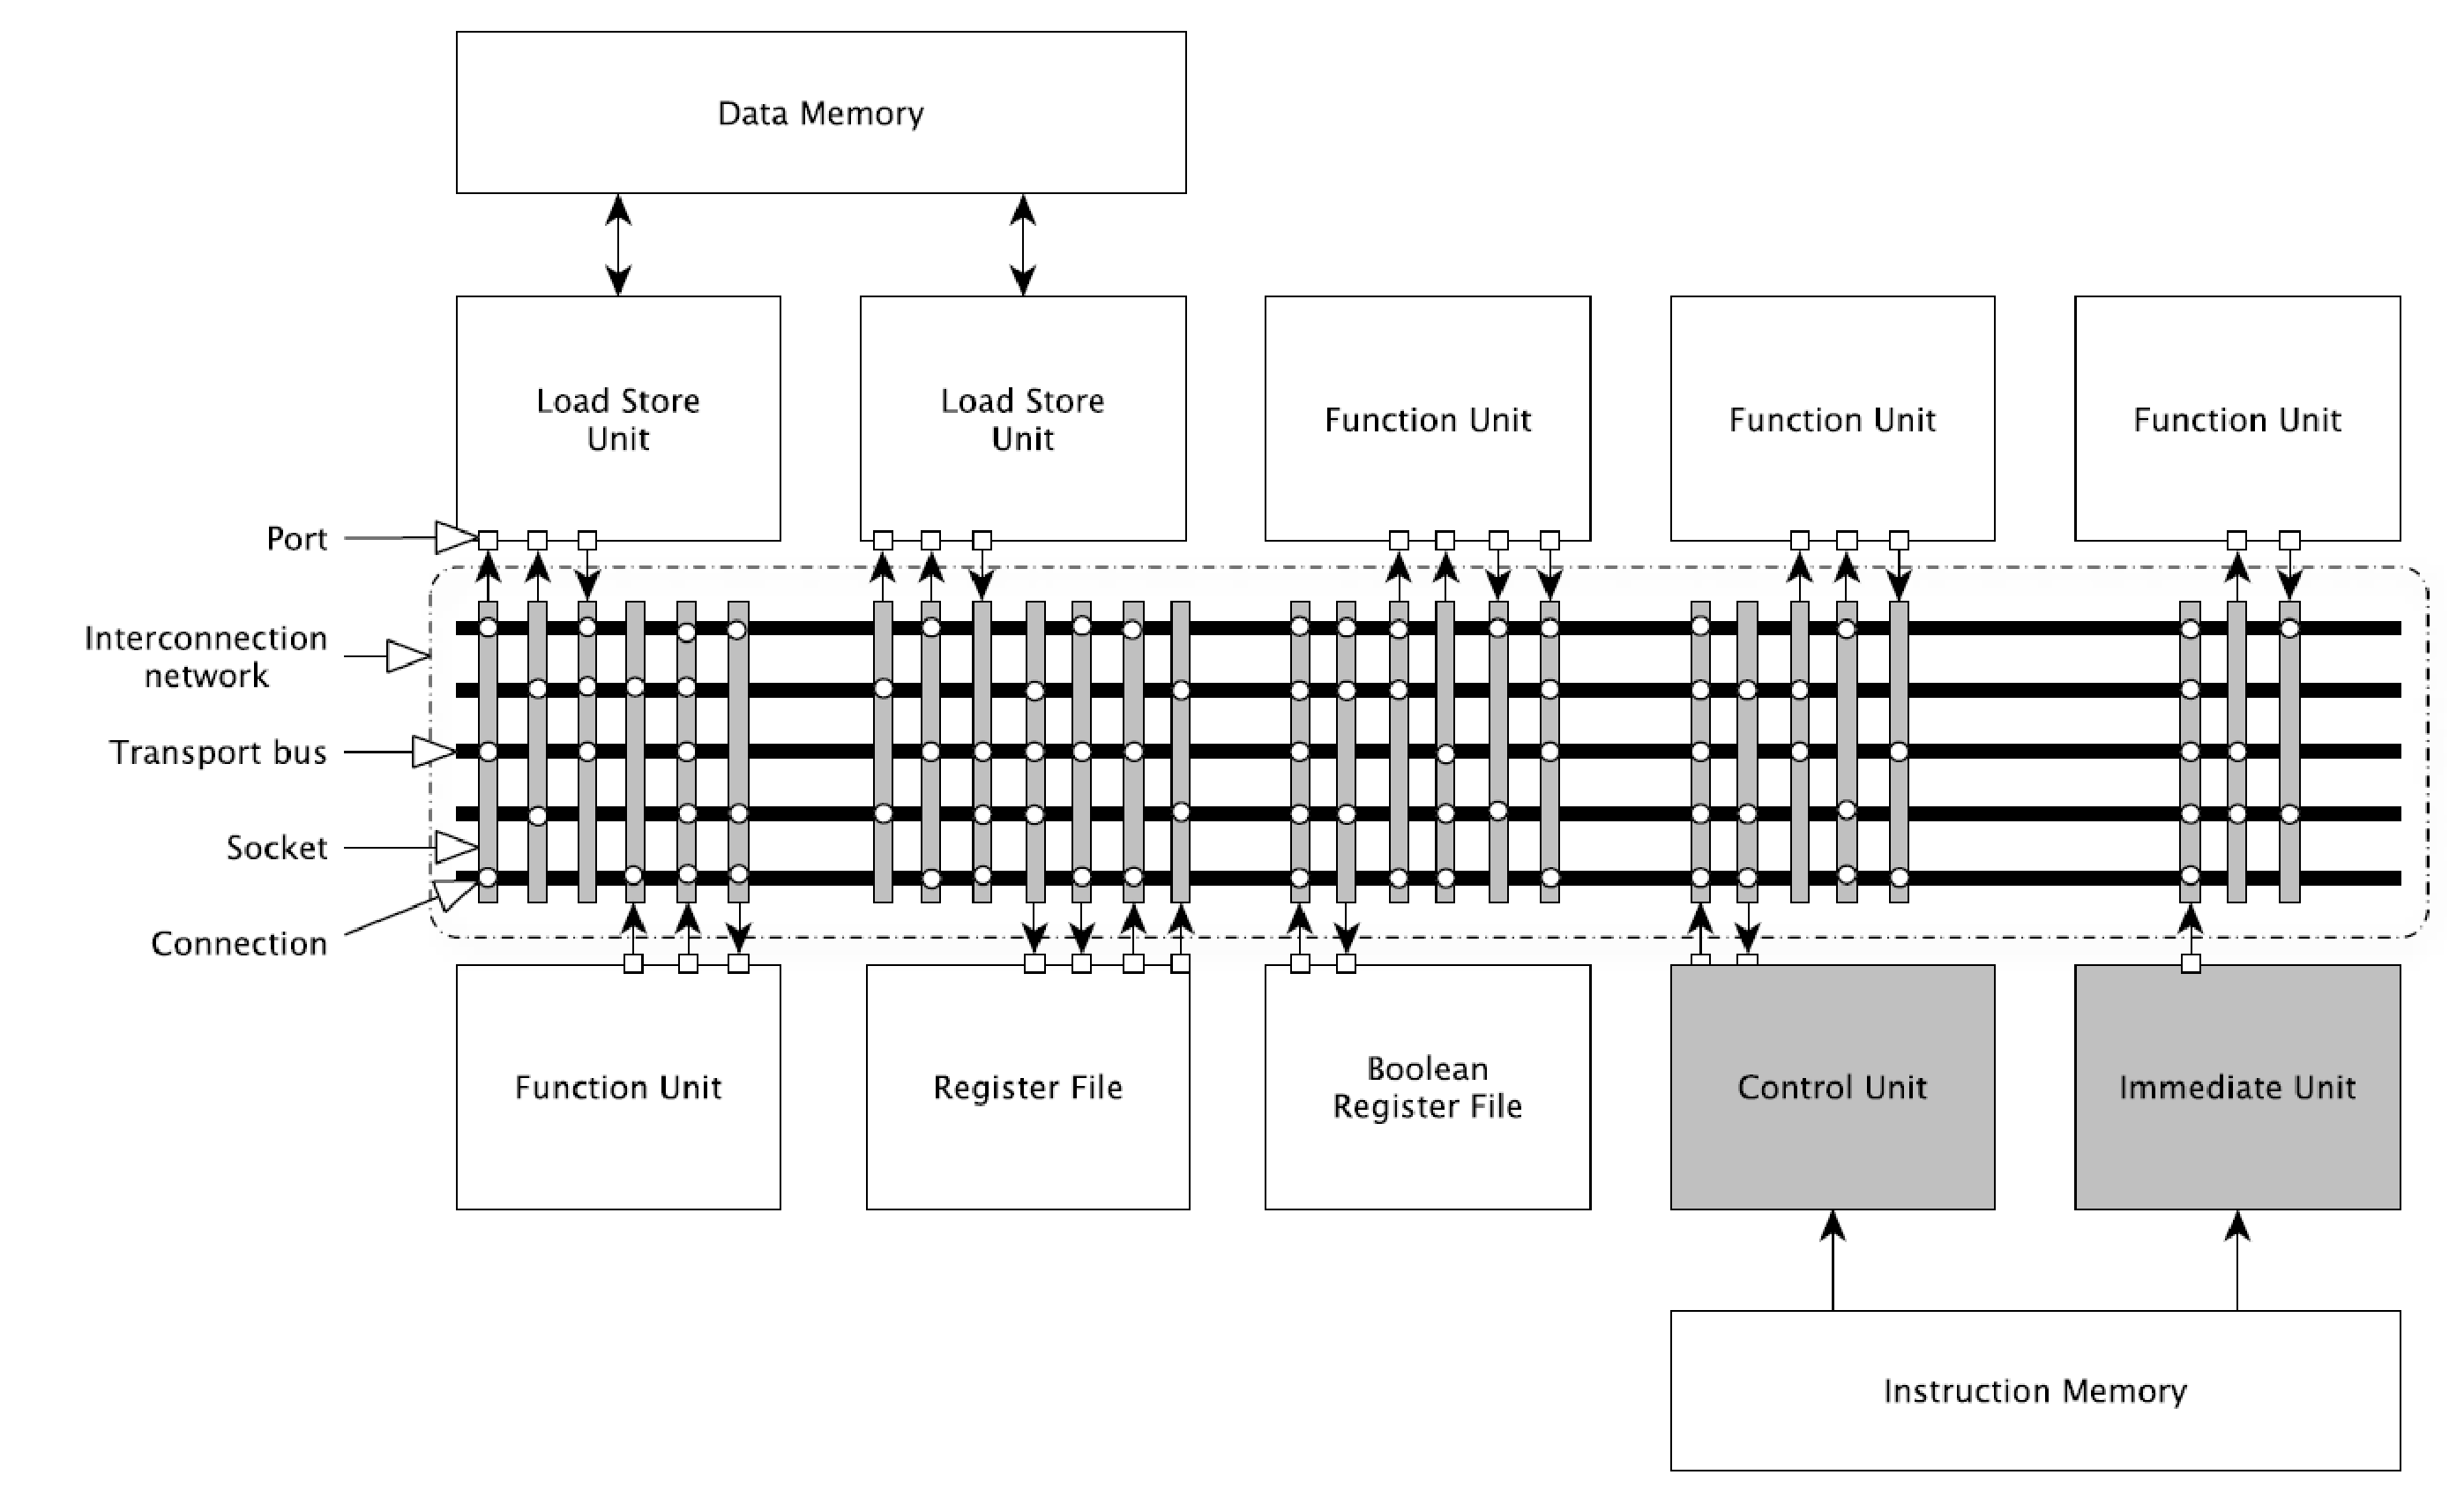
\includegraphics[width=0.75\textwidth]{eps/tta}
	\caption{TTA basic structure} 
	\label{fig:tta1} 
  \end{center}
\end{figure}

In a basic case, all FU input and output ports are registers which
relieves the pressure on the register file. Thanks to the programming
model, operands can be bypassed directly from one FU to another. This
is called software bypassing. Additionally, if the bypassed operand is
not needed by anyone else there is no need to write the operand to a
register file. This optimization technique is called dead result
elimination. Combining software bypassing with dead result elimination
helps to reduce register file traffic.  Moreover, the TCE TTA template
gives freedom for partitioning register files. For example, there can
be several small and simple register files instead one centralized
multiported RF.

The transport programming is also beneficial because it allows easy
scalability of the architecture and compiler, as well as supports
varying pipeline depths at FUs. At the same time, the number of FU
inputs and outputs is not restricted, unlike in most processor
templates which support only instructions with 2 inputs and 1
output value. User can also create instruction set extensions with a
\textit{special function unit} (SFU) which can have arbitrary number
of I/O operands. Instruction set extension is a powerful way of
enhancing the performance of certain applications.

\begin{table}
  \begin{center}
    \caption {Configurable aspects of the TCE's TTA template}
    \label {tab:filetypes}
    \begin{tabular}{l | l | l }
      \hline
      Property & Values & Example  \\
      \hline
      \hline
      Functional unit         & Type, count                         & 3x ALU, 2x LSU, 1x MUL, 1x ctrl...\\
      Register file (RF)      & \# registers, \#RFs, \#ports, width & 16x 32b RF 2x rd + 2x wr ports, 16x 1b boolean RF \\
      Interconnection network & \#buses, \#sockets                & 5 buses, total of 43 write and 44 read sockets\\
      Memory interfaces       & Count, type                       & 2x LSU for SRAM w/ 32b data \& 32b addr \\
      Special FU              & User-defined functionality        & dct, semaphor\_lock, FIFO I/O \\
      \hline
    \end{tabular}
  \end{center}
\end{table}

\subsection{Immediates/Constants}

The TTA template supports two ways of transporting program constants
in instructions, such as \textit{``add value+5''}. \textit{Short
  immediates} are encoded in the move slot's source field, and thus
consume a part of a single move slot. The constants transported in the
source field should usually be relatively small in size, otherwise the
width of a move slot is dominated by the immediate field.

Wider constants can be transported by means of so called \textit{long
  immediates}. Long immediates can be defined using an ADF parameter
called \textit{instruction template}. The instruction template defines
which slots are used for pieces of the instruction template or for
defining the transports (moves).  The slots cannot be used for regular
data transports when they are used for transporting pieces of a long
immediate.

An instruction template defining a long immediate also provides
a target to which the long immediate must be transported. The target register
resides in a so called \textit{immediate unit} which is written directly 
from the control unit, not through the transport buses. The immediate unit is like
a register file expect that it contains only read ports and is written
only by the instruction decoder in the control unit when it detects an 
instruction with a long immediate (see Fig.~\ref{fig:tta1}).

Thus, in order to support the special long immediate encoding, one has
to add a) an instruction template that supports transporting the pieces
of the immediate using full move slots b) at least one long immediate
unit (a read-only register file) to which the instruction writes the
immediates and of which registers the immediates can be read to the
datapath.

\subsection{Operations, Function Units, and Operand Bindings}
Due to the way TCE abstracts operations and function units, an
additional concept of \textit{operand binding} is needed to 
connect the two in processor designs.

Operations in TCE are defined in a separate database (OSAL,
Sections~\ref{section:osal} and \ref{section:osal_details} ) in order
to allow defining a reusable database of ``operation semantics''. The
operations are used in processor designs by adding \textit{function
units} (FU) that implement the wanted operations. Operands of the
operations can be mapped to different ports of the implementing FU,
which affects programming of the processor. Mapping of operation
operands to the FU ports must be therefore described by the processor
designer explicitly.

\textbf{Example.} Designer adds an FU called 'ALU' which implements
operations 'ADD', 'SUB', and 'NOT'. ALU has two input ports called 'in1' and 
'in2t' (triggering), and an output port called 'out'. A logical binding of 
the 'ADD' and 'SUB' operands to ALU ports is the following:

\begin{verbatim}
 ADD.1 (the first input operand) bound to ALU.in1
 ADD.2 (the second input operand) bound to ALU.in2t
 ADD.3 (the output operand) bound to ALU.out

 SUB.1 (the first input operand) bound to ALU.in1
 SUB.2 (the second input operand) bound to ALU.in2t
 SUB.3 (the output operand) bound to ALU.out
\end{verbatim}

However, operation 'NOT', that is, the bitwise negation has only one input
thus it must be bound to port 'FU.in2t' so it can be triggered:

\begin{verbatim}
 NOT.1 bound to ALU.in2t
 NOT.2 (the output operand) bound to ALU.out
\end{verbatim}

Because we have a choice in how we bind the 'ADD' and 'SUB' input operands,
the binding has to be explicit in the architecture definition. The operand
binding described above defines architecturally different TTA function unit
from the following:

\begin{verbatim}
 SUB.2 bound to ALU.in1
 SUB.1 bound to ALU.in2t
 SUB.3 bound to ALU.out
\end{verbatim}

With the rest of the operands bound similarly as in the first example.

Due to the differing 'SUB' input bindings, one cannot run code scheduled
for the previous processor on a machine with an ALU with the latter 
operand bindings. This small detail is important to understand when 
designing more complex FUs, with multiple operations with different number of 
operands of varying size, but is usually transparent to the basic user of 
TCE.

Reasons for wanting to fine tune the operand bindings might include using
input ports of a smaller width for some operation operands. For example, the 
width of the address operands in memory accessing operations of a load store 
unit is often smaller than the data width. Similarly, the second operand of
a shift operation that defines the number of bits to shift requires less
bits than the shifted data operand.


\subsection{Datapath Connectivity Levels}
\label{ConnectivityLevels}
The datapath interconnection network of TTAs is visible to the
programmer (i.e. the compiler in practice).  This enables full
customization of the connectivity, making it possible to remove
connections that are rarely, if at all, used by the programs the
processor at hand is designed to run. This offers notable saving in
the HW area. However, the less connections the machine has, the more
challenging it becomes to automatically produce efficient code for
it. This section describes the different TTA ``connectivity levels''
and their support in the TCE design flow.

The currently identified and supported connectivity levels are, in the order of 
descending level of connectivity, as follows:
\begin{enumerate}

\item Fully connected. Completely connected interconnection network ``matrix''.
All bus-socket and socket-port connections are there. There is a shortcut for
creating this type of connectivity in the ProDe tool.

The easy target for the high-level language compiler tcecc. However, not
a realistic design usually due to its high implementation costs.

\item Directly reachable. The connectivity has been reduced. However, there is
still at least one direct connection from each function unit (FU) and register file 
(RF) output to all inputs.

An easy target for tcecc.

\item Fully RF connected. All FUs are connected to all RFs. That is, you can 
read and write any general purpose register (GPR) from any FU with a single
move. However, some or all bypass connections between FUs might be missing.

An easy target for tcecc. However, reduction of bypass connections means
that less software bypassing can be done.

\item Reachable. All FUs are connected to at least one RF and all RFs (and thus
other FUs) can be reached via one or more additional register copy moves. 

Compilation is fully supported by tcecc. The number of copies is not 
limited by tcecc. However, this style of connectivity results in suboptimal code due to the
additional register copies which introduce additional moves, consume registers, and
produce dependencies to the code which hinder parallelism.

\item RF disconnected. Some FUs are not connected to any RF or there are 
``separated islands'' without connectivity to other ``islands''.

Not supported by tcecc. However, any connectivity type is supported by 
the TCE assembler. Thus, one can resort to manual TTA assembly programming in
this case.

\end{enumerate}

\section{Programmer Interface}

This section describes the programmer interface, which is 
the application binary interface followed by tcecc.

The programs produced by tcecc are fully linked and not expected
to be relinked afterwards to other programs. Therefore, details 
such as the function calling convention can be customized per program by 
the compiler. For these parts, this section describes the current 
default behavior for reference.

\subsection{Default Data Address Space Layout}
\label{ssec:address-spaces-of-umach}

When compiling from a higher-level language using tcecc, there 
has to be at least one byte-addressible data address space in the machine. 
This is the ``default address space'', marked with the numerical 
id 0 in case there are multiple data address spaces. 

The C/C++ compilation lays out the global variables starting from the 
first data memory location to the default address space. The first 
location after the global variables is the start location for heap, 
in case the program uses dynamic memory allocation. It grows upwards. 
The stack, used to store the function local variables and to pass 
parameters in the function calls, grows from the largest memory address 
downwards. The start address of the stack can be changed with the tcecc 
switch \textit{{--}init-sp}.

As both heap and stack grow dynamically towards each other, to way to
increase the available space for heap/stack is to 
increase the size of your data memory address space in ADF. 

\subsection{Instruction Address Space}

The default GCU assumes that instruction memory is intruction addressable. In
other words the instruction word must fit in the MAU of the instruction
memory. This way the next instruction can be referenced by incrementing the
current program counter by one.

How to interface the instruction memory with an actual memory chip is out of
scope in TCE because there are too many different platforms and chips and
possibilities. But as an advantage this gives the user free hands to
implement almost any kind of memory hierarchy the user wants. Most probably
you must implement a memory adapter to bind the memory chip and the TTA
processor interfaces together.

\subsection{Alignment of Words in Memory}
\label{ssec:align-conventions}

tcecc aligns the addresses of data word to the data type size in bytes.
For example, if a floating-point word takes 4 MAU's, its address must be 
a multiple of 8. 

The memory acessing operations in the base operation set (ldq, ldh, ldw,
ldd, stq, sth, stw, and ldd) are aligned with their size. Operations stq/ldq
are for accessing single bytes, thus their alignment is 1 byte, 
for sth/ldh it is 2 bytes, and for stw/ldw it is 4 bytes. Thus, one cannot 
assume to be able to access, for example, a 4 byte word at address 3
using stw/ldw.

Double precision floating point word operations std/ldd which access
64-bit words are aligned at 8-byte addresses. 

The effect of misaligned word accesses on processor implementations are
undefined. Typically: (1) the processor accesses the nearest (lower) aligned
address instead (because of zeroing the lower address bits); (2) the processor 
halts or rises an exception (unlikely). More likely is that, a processor 
could enter a slower operation mode and perform a mis-aligned memory access.
However, these behaviors are not \textit{required} by the above mentioned 
aligned base memory operations shipped with TCE.

\subsection{Stack Frame Layout}
\label{sec:stack-layout}

The register assigned to act as the stack pointer register (referred to as 
SPR) is the register number 0 of the first 32b register file in the ADF. 
There is no frame pointer.

\begin{figure}[t]
  \centerline{
  \psfig{figure=eps/StackFrame.eps,width=9.75cm}
  }
  \caption{Stack layout for a situation with two call frames, A() calling B().}
  \label{fig:stack-frame}
\end{figure}

The stack of a program is divided up into blocks of contiguous memory called
\emph{frames}. Each frame is activated upon entering a function and is
destroyed (its storage is made available for new frames) when that function
invocation returns. The stack frame of a function contains the arguments
with which the function is called and variables local to the procedure.

The stack pointer register (SPR) always points to the the first word past
the area of the current frame that is dedicated to local variables.  The
area of the stack past the local variables area contains the outgoing
arguments of called functions (if any).  The stack of TTA's supported by TCE
grows downwards, therefore the incoming arguments and the local variables on
the local stack frame have positive offsets when accessed from the current
function, whereas the outgoing arguments have negative stack offsets.

Figure~\ref{fig:stack-frame} depicts the memory layout of part of a TTA
stack that contains two frames: A and B.  When function A frame is
activated, SPR points to the first word past the top of the local variable
area of the caller frame (this location is shown as ``SPR'' in figure).  At
function entry and before accessing the stack, function A initialises SPR
with the top of its frame (shown as ``SPR-A'' in figure).  When function A
prepares a call to function B, it sets up the outgoing arguments in the
stack area past its local variable area.  At function entry, function B
initialises SPR with the first word past the top of its local variable area
(shown as ``SPR-B'' in figure).  In case function B does not use any stack
for passing outgoing arguments, the location SPR-B corresponds to one word
past the top of the frame.

The value of the return address register is pushed to stack before the 
function's local variables in case the function is not a leaf function
(a function without calls to other functions). If the called function returns 
an object that does not fit to the return value register, the function 
gets an implicit argument that points to the location in the callee's 
stack where the return value object will be written by the called function. 

\subsection{Word Byte Order}
\label{ssec:word-order}

TCE-TTA processors follow the big endian byte order.

\subsection{Function Calling Conventions}
\label{ssec:calling-conventions}

The current default calling convention generated by tcecc is as follows.

The register number 1 in the first 32b register file of ADF 
is a return value register which is used to return 
32b values such as $int$s or $float$s from functions. 
The same register is reused for the first 
passed parameter value in function calls, if suitable. 

In a function call, the arguments and return values that do not fit 
in the 32b return value / parameter register are pushed to stack.

The return location for the last executed CALL operation is 
stored in the RA register in the control unit. This is pushed 
to stack in case of multiple function call layers. Refer to the 
stack frame layout for more information.


\subsection{Register Context Saving Conventions}
\label{ssec:register-conventions}

All registers except SPR may have to be saved and restored as a result of a
function call.  When a register carries a variable in the caller code that
remains live across a function call, and uses a register overwritten in the callee, 
it needs to be saved and restored.  Registers are subdivided in two groups:
those that are saved and restored around a function call site, and those that are
saved at the beginning of the called function and are restored before it 
returns. The first group is termed \textit{caller-saved} registers, the second 
group \textit{callee-saved} registers.

The compiler has the freedom to optimize the context saving convention.
Depending on the properties of the program and the capacity of the register
allocator, a varying fraction of the total GPR's in a register file may be
assigned to either above mentioned groups.  The register allocator may even 
dedicate one register file completely to caller-saved registers and another 
to callee-saved registers.

The current default register saving convention followed by tcecc is to have 
treat all registers as caller saved. 

\chapter{PRODUCING EFFICIENT TTA DESIGNS WITH TCE}

This chapter gives some tips on how to avoid the most common bottlenecks that
often arise in the TTA designs produced using TCE and how to get good 
performance for your architecture.

\section{Registers and Register Files}

Make sure you have enough general purpose registers and register file 
read ports. Using more than two read ports in one register file may make it 
big, slow and power-hungry, so consider splitting the RF to multiple register files.

However, it should be noted that the current compiler does not perform
intelligent distribution of variables to the register files, so if the machine
is not equally connected to all the function units that consume each variable,
you might end up with ``connectivity register copies'' (see below). The current 
register distribution method is \textit{round robin} which balances the RF load somewhat,
but not perfectly, as it doesn't take in account the computation that uses each 
variable. 

To produce better register distribution, the compiler should balance the RF load at 
the granularity of ``computation trees'', not at the granularity of a single register
to produce more parallelizable code and to reduce register copies. Improving this 
part of the code generation is being worked on with high priority.

\section{Interconnection Network}

See Section~\ref{ConnectivityLevels} for the definitions of the different
connectivity classes of the TTAs designed with TCE.

Some additional points worth considering:

\begin{itemize}
\item
'Fully connected' on architectures that are not very small usually lead to 
low maximum clock frequencies.

\item
Having only the 'Reachable' connectivity leads to the need to add extra
register-to-register transfers created by the compiler and may cause
considerable slowdowns due to the difficulties to parallelize such code.

\end{itemize}

The best compromize between \textit{instructions-per-cycle (IPC)} and clock speed 
is usually 'Fully RF connected' with additional FU to FU connections for commonly 
used bypasses.

This, of course, doesn't always hold. For example, if the clock speed is limited by some
other component than the interconnect, Directly Reachable might give
slightly better performance. Sometimes some architecture with only 
'Reachable' connectivity might give so big clocks speed improvement that
it might outweight the IPC penalty. So, it needs some experimenting from
the designer as it depends on the parallelism of the program among other things.

With some future improvements to the compiler the performance of 'Reachable'
architectures may get a definite improvement, at which point we'll update these
hints.

There is a tool called ConnectionSweeper which can be used to optimize the
interconnection network automatically. ConnectionSweeper is documented in 
Section~\ref{ConnectionSweeper}.

\subsection{Negative short immediates}

Make sure you have one or more buses (actually ``move slots``) with signed short 
immediate fields. Small negative numbers such as -1, and -4 are very common in 
the generated code, and long immediates often cause bottlenecks on the machine code.

\section{Operation Set}

Optimize your operation set for your code. Make sure you support the 
performance-critical instructions with hardware operations. Software-emulation of 
some operations is usually 50-100 times slower than hardware execution and
might prevent parallelization of multiple iterations of the core kernel loop.

For example, if you do a lot of floating point calculations, use hardware floating 
point units. If your inner loop contains integer multiplications, put a multiplier in 
your architecture.

On the other hand, if you do not need a floating point unit, integer multiplier or 
a divider, do not put them to your achitecture ``just in case'', as they increase 
the size of the processor, power consumption, and also the size of the instruction 
word. It also makes the interconnection network more complex which often also 
reduces the clock speed and therefore performance. Unless, of course, you need
the ``general purposity`` and you predict that some of the future programs that 
are going to run in your processor might be able to exploit such hardware units.

After your selection of basic operations is good for your program, and you still 
need more performance or lower power consumption, then consider using custom 
operations. 

\chapter{TROUBLESHOOTING}
\label{chapter:troubleshooting}

This chapter gives solutions to common problems encountered while using TCE.

\section{Simulation}

Problems with simulation, both with command line (ttasim) and graphical
user interfaces (proxim) are listed here.

\subsection{Failing to Load Operation Behavior Definitions}

It might be possible that you have defined some custom operations to
\verb|~/.tce/opset/custom| which conflict with your new definitions, or the
simulation behaviors are compiled with an older compiler and not compatible
with your new compiler. Workaround for this is to either delete the old
definitions or rebuild them.

\section{Limitations of the Current Toolset Version}

This section lists the most user-visible limitations placed by the current
toolset version.

\subsection{Integer Width}

The simulator supports only integer computations with maximum word width of
32 bits. 

\subsection{Instruction Addressing During Simulation}

The details of encoding and compression of the instruction memory are not
taken into account before the actual generation of the bit image of the
instruction memory. This decision was taken to allow simplification in the
other parts of the toolset, and to allow easy "exploration" with different
encodings and compression algorithms in the bit generation phase.

This implies that every time you see an instruction address in
architectural simulation, you are actually seeing an instruction index.
That is, instruction addressing (one instruction per instruction memory
address) is assumed.

We might change this in the future toolset versions to allow seeing exact
instruction memory addresses during simulation, if that is seen as a
necessity. Currently it does not seem to be a very important feature.

\subsection{Data Memory Addressing}

There is no tool to map data memory accesses in the source code to the
actual target's memories. Therefore, you need to have a data memory which
provides byte-addressing with 32-bit words. The data will be accessed using
operations LDQ, LDH, LDW, STQ, STH, STW, which access the memory in 1 (q),
2 (h), and 4 (w) byte chunks. This should not be a problem, as it is rather
easy to implement byte-addressing in case the actual memory is of width of
2's exponent multiple of the byte. The parallel assembler allows any kind
of minimum addressable units (MAU) in the load/store units. In that case,
LDQ/STQ just access a single MAU, etc. One should keep in mind the 32-bit
integer word limitation of simulation. Thus, if the MAU is 32-bits, one
cannot use LDH or LDW because they would require 64 and 128 bits,
respectively.

\subsection{Ideal Memory Model in Simulation}

The simulator assumes ideal memory model which generates no stalls and
returns data for the next instruction. This so called 'Ideal SRAM' model
allows modeling all types of memories in the point of view of the
programmer. It is up to the load/store unit implementation to generate the
lock signals in case the memory model does not match the ideal model.

There are hooks for adding more memory models which generate lock signals
in the simulation, but for the v1.0 the simulator does not provide other
memory models, and thus does not support lock cycle simulation.

\subsection{Guards}

The guard support as specified in the ADF specification~\cite{ADF-specs} is
only partially supported in TCE. `Operators other than logical negation are
not supported. That is, supported guards always ``watch'' a single register
(FU output or a GPR). In addition, the shipped default scheduling algorithm
in compiler backend requires a register guard. Thus, if more exotic guarded
execution is required, one has to write the programs in parallel assembly
(Section~\ref{section:TCEAsm}).

\subsection{Operation Pipeline Description Limitations}

Even though supported by the ADF and ProDe, writing of operands after
triggering an operation is not supported neither by the compiler nor
the simulator. However, setting different latencies for outputs of 
multi-result operations is supported. For example, using this
feature one can have an iterative operation pipeline which computes 
several results which are ready after the count of stages in an iteration.

\subsection{Encoding of XML Files}

TCE uses XML to store data of the architectures and implementation 
locations (see Section~\ref{sec:adf} and Section~\ref{sec:idf}). The
encoding of the XML files must be in 7-bit ascii. If other encodings are
used, the result is undefined.

\subsection{Floating Point Support}

The simulator supports the half (16 bits), single (32 bits) and double
(64 bits) precision floating point types. However, at this time only
single precision float operations (ADDF, MULF, etc.) are selected 
automatically when starting from C/C++ code. Currently, the compiler 
converts doubles to floats to allow compiling and running code with 
doubles with reduced precision.

\appendix

\chapter{FREQUENTLY ASKED QUESTIONS}
\label{chapter:faq}

\section{Memory Related}

Questions related to memory accessing.

\subsection{Load Store Unit}

In the LSU implementations shipped with TCE the two LSB bits are used by the LSU to control
a so called write mask that handles writing of bytes. This means that the
memory address outside the processor is 2 bits narrower than inside the
processor. When you set the data address space width in ProDe, the width
is the address width inside the processor.


\section{Processor Generator}

\subsubsection{Warning: Processor Generator failed to generate a test bench}
The automatic testbench generator currently does not support any special
function units that connect signals out from toplevel.vhdl. This warning
can be ignored if you are not planning to use the automatically generated
test bench.

\subsubsection{Warning: Opcode defined in HDB for operation ...}

Processor Generator gives a warning message if the operation codes in FU
are not numbered according to the alphabetical order of the operations.
The VHDL implementation and the HDB entry of the FU should be fixed to use 
this kind of opcode numbering. See section \ref{sec:opcodeorder} for more 
details.

\section{tcecc}

\subsubsection{Disappearing code}

Tcecc is using the efficient LLVM compiler framework for its optimizations.
Sometimes LLVM is too aggressive and removes code that you might not
intend to get removed. This happens in case you write your output to a
global variable which you might dump only in the simulator and never read 
it in your program nor e.g. print it with \textbf{printf()}. In this case 
LLVM sees writes to a global variable which is never read by the program, 
thus thinks the computation producing the written value is useless and 
removes it as dead code.

A solution to the problem is to always mark the global ``output/verification'' 
variables as 'volatile' which means that the content of the variable should 
be always written to the memory. Thus, LLVM has to assume that there might 
be other readers of the same variable that are just not visible in the 
current program.

\section{Hardware characteristics}

\subsection{Interrupt support}

Currently TCE does not have support for TTA interrupts. This is mostly due to
the fact that context saving is an expensive operation on TTA because the
processor context can be huge. In general, TTA might not be the best
architecture choice for the only processor in a control-oriented or reactive 
system.

\section{Misc}

\subsection{File Search Paths}

The tools in TCE search for files such as HDBs and OSAL operation definitions,
in addition to the TCE install locations, in the current working directory and
its 'data' subdirectory. 

\chapter{SystemC Simulation Example}
\label{appendix:SystemCExample}

This SystemC simulation example simulates a system with two TTA cores
communicating through two shared registers with memory mapped access.
One of the registers (busyReg) is used to denote that the ``receiver TTA'' is
busy processing the previously written data which the ``sender TTA'' writes
(to dataReg). The receiver uses \textbf{iprintf} to print out the received data.

The C source codes for the programs running in the two TTAs 
are shown below:. \textbf{mem\_map.h} defines constants for the memory 
mapped I/O addresses. This file is 
included by both TTA programs and the SystemC simulation code presented
later.

\textbf{mmio\_recv.c: The C program running in the receiver TTA:}

\verbatiminput{systemc_example/mmio_recv.c}

\textbf{mmio\_send.c: The C program running in the sender TTA.}
\verbatiminput{systemc_example/mmio_send.c}

\textbf{mem\_map.h: The memory mapped I/O addresses as constants:}
 
\verbatiminput{systemc_example/mem_map.h}

The simple register is defined in \textbf{register.hh} and the
load-store unit simulation model that overrides the default TTA simulator
one in \textbf{lsu\_model.hh}.

\textbf{register.hh: SystemC model for an integer register:}
 
\verbatiminput{systemc_example/register.hh}

\textbf{lsu\_model.hh: The load-store unit model for the TTAs:}

\verbatiminput{systemc_example/lsu_model.hh}

Finally, the actual main SystemC simulation code is defined as follows.
As can be noted, both of the TTA cores use the same architecture loaded from
\textbf{mmio.adf} of which contents are not presented here. In order to 
make this example work, the TCE-included \textbf{minimal\_with\_io.adf} 
architecture can be used instead.

\textbf{simulator.cc: The main simulation code:}
 
\verbatiminput{systemc_example/simulator.cc}

The simulator can be compiled with the following command (assuming gcc
used):

\begin{verbatim}
g++ `tce-config --includes --libs` simulator.cc -lsystemc -O3 -o simulator
\end{verbatim}

The simulation should produce output similar to the following:

\begin{verbatim}
./simulator

             SystemC 2.2.0 --- Aug 30 2010 13:05:02
        Copyright (c) 1996-2006 by all Contributors
                    ALL RIGHTS RESERVED
mmio_recv got 1234
mmio_recv got 3702
mmio_recv got 4936
mmio_recv got 6170
mmio_recv got 7404
mmio_recv got 9872
mmio_recv got 12340
\end{verbatim}


\chapter{Copyright notices}

Here are the copyright notices of the libraries used in the software.

\section{Xerces}

Xerces-C++ is released under the terms of the Apache License, version
2.0.  The complete text is presented here.


                                 Apache License
                           Version 2.0, January 2004
                        http://www.apache.org/licenses/

   TERMS AND CONDITIONS FOR USE, REPRODUCTION, AND DISTRIBUTION

   1. Definitions.

      "License" shall mean the terms and conditions for use, reproduction,
      and distribution as defined by Sections 1 through 9 of this document.

      "Licensor" shall mean the copyright owner or entity authorized by
      the copyright owner that is granting the License.

      "Legal Entity" shall mean the union of the acting entity and all
      other entities that control, are controlled by, or are under common
      control with that entity. For the purposes of this definition,
      "control" means (i) the power, direct or indirect, to cause the
      direction or management of such entity, whether by contract or
      otherwise, or (ii) ownership of fifty percent (50%) or more of the
      outstanding shares, or (iii) beneficial ownership of such entity.

      "You" (or "Your") shall mean an individual or Legal Entity
      exercising permissions granted by this License.

      "Source" form shall mean the preferred form for making modifications,
      including but not limited to software source code, documentation
      source, and configuration files.

      "Object" form shall mean any form resulting from mechanical
      transformation or translation of a Source form, including but
      not limited to compiled object code, generated documentation,
      and conversions to other media types.

      "Work" shall mean the work of authorship, whether in Source or
      Object form, made available under the License, as indicated by a
      copyright notice that is included in or attached to the work
      (an example is provided in the Appendix below).

      "Derivative Works" shall mean any work, whether in Source or Object
      form, that is based on (or derived from) the Work and for which the
      editorial revisions, annotations, elaborations, or other modifications
      represent, as a whole, an original work of authorship. For the purposes
      of this License, Derivative Works shall not include works that remain
      separable from, or merely link (or bind by name) to the interfaces of,
      the Work and Derivative Works thereof.

      "Contribution" shall mean any work of authorship, including
      the original version of the Work and any modifications or additions
      to that Work or Derivative Works thereof, that is intentionally
      submitted to Licensor for inclusion in the Work by the copyright owner
      or by an individual or Legal Entity authorized to submit on behalf of
      the copyright owner. For the purposes of this definition, "submitted"
      means any form of electronic, verbal, or written communication sent
      to the Licensor or its representatives, including but not limited to
      communication on electronic mailing lists, source code control systems,
      and issue tracking systems that are managed by, or on behalf of, the
      Licensor for the purpose of discussing and improving the Work, but
      excluding communication that is conspicuously marked or otherwise
      designated in writing by the copyright owner as "Not a Contribution."

      "Contributor" shall mean Licensor and any individual or Legal Entity
      on behalf of whom a Contribution has been received by Licensor and
      subsequently incorporated within the Work.

   2. Grant of Copyright License. Subject to the terms and conditions of
      this License, each Contributor hereby grants to You a perpetual,
      worldwide, non-exclusive, no-charge, royalty-free, irrevocable
      copyright license to reproduce, prepare Derivative Works of,
      publicly display, publicly perform, sublicense, and distribute the
      Work and such Derivative Works in Source or Object form.

   3. Grant of Patent License. Subject to the terms and conditions of
      this License, each Contributor hereby grants to You a perpetual,
      worldwide, non-exclusive, no-charge, royalty-free, irrevocable
      (except as stated in this section) patent license to make, have made,
      use, offer to sell, sell, import, and otherwise transfer the Work,
      where such license applies only to those patent claims licensable
      by such Contributor that are necessarily infringed by their
      Contribution(s) alone or by combination of their Contribution(s)
      with the Work to which such Contribution(s) was submitted. If You
      institute patent litigation against any entity (including a
      cross-claim or counterclaim in a lawsuit) alleging that the Work
      or a Contribution incorporated within the Work constitutes direct
      or contributory patent infringement, then any patent licenses
      granted to You under this License for that Work shall terminate
      as of the date such litigation is filed.

   4. Redistribution. You may reproduce and distribute copies of the
      Work or Derivative Works thereof in any medium, with or without
      modifications, and in Source or Object form, provided that You
      meet the following conditions:

      (a) You must give any other recipients of the Work or
          Derivative Works a copy of this License; and

      (b) You must cause any modified files to carry prominent notices
          stating that You changed the files; and

      (c) You must retain, in the Source form of any Derivative Works
          that You distribute, all copyright, patent, trademark, and
          attribution notices from the Source form of the Work,
          excluding those notices that do not pertain to any part of
          the Derivative Works; and

      (d) If the Work includes a "NOTICE" text file as part of its
          distribution, then any Derivative Works that You distribute must
          include a readable copy of the attribution notices contained
          within such NOTICE file, excluding those notices that do not
          pertain to any part of the Derivative Works, in at least one
          of the following places: within a NOTICE text file distributed
          as part of the Derivative Works; within the Source form or
          documentation, if provided along with the Derivative Works; or,
          within a display generated by the Derivative Works, if and
          wherever such third-party notices normally appear. The contents
          of the NOTICE file are for informational purposes only and
          do not modify the License. You may add Your own attribution
          notices within Derivative Works that You distribute, alongside
          or as an addendum to the NOTICE text from the Work, provided
          that such additional attribution notices cannot be construed
          as modifying the License.

      You may add Your own copyright statement to Your modifications and
      may provide additional or different license terms and conditions
      for use, reproduction, or distribution of Your modifications, or
      for any such Derivative Works as a whole, provided Your use,
      reproduction, and distribution of the Work otherwise complies with
      the conditions stated in this License.

   5. Submission of Contributions. Unless You explicitly state otherwise,
      any Contribution intentionally submitted for inclusion in the Work
      by You to the Licensor shall be under the terms and conditions of
      this License, without any additional terms or conditions.
      Notwithstanding the above, nothing herein shall supersede or modify
      the terms of any separate license agreement you may have executed
      with Licensor regarding such Contributions.

   6. Trademarks. This License does not grant permission to use the trade
      names, trademarks, service marks, or product names of the Licensor,
      except as required for reasonable and customary use in describing the
      origin of the Work and reproducing the content of the NOTICE file.

   7. Disclaimer of Warranty. Unless required by applicable law or
      agreed to in writing, Licensor provides the Work (and each
      Contributor provides its Contributions) on an "AS IS" BASIS,
      WITHOUT WARRANTIES OR CONDITIONS OF ANY KIND, either express or
      implied, including, without limitation, any warranties or conditions
      of TITLE, NON-INFRINGEMENT, MERCHANTABILITY, or FITNESS FOR A
      PARTICULAR PURPOSE. You are solely responsible for determining the
      appropriateness of using or redistributing the Work and assume any
      risks associated with Your exercise of permissions under this License.

   8. Limitation of Liability. In no event and under no legal theory,
      whether in tort (including negligence), contract, or otherwise,
      unless required by applicable law (such as deliberate and grossly
      negligent acts) or agreed to in writing, shall any Contributor be
      liable to You for damages, including any direct, indirect, special,
      incidental, or consequential damages of any character arising as a
      result of this License or out of the use or inability to use the
      Work (including but not limited to damages for loss of goodwill,
      work stoppage, computer failure or malfunction, or any and all
      other commercial damages or losses), even if such Contributor
      has been advised of the possibility of such damages.

   9. Accepting Warranty or Additional Liability. While redistributing
      the Work or Derivative Works thereof, You may choose to offer,
      and charge a fee for, acceptance of support, warranty, indemnity,
      or other liability obligations and/or rights consistent with this
      License. However, in accepting such obligations, You may act only
      on Your own behalf and on Your sole responsibility, not on behalf
      of any other Contributor, and only if You agree to indemnify,
      defend, and hold each Contributor harmless for any liability
      incurred by, or claims asserted against, such Contributor by reason
      of your accepting any such warranty or additional liability.

   END OF TERMS AND CONDITIONS

   APPENDIX: How to apply the Apache License to your work.

      To apply the Apache License to your work, attach the following
      boilerplate notice, with the fields enclosed by brackets "[]"
      replaced with your own identifying information. (Do Not include
      the brackets!)  The text should be enclosed in the appropriate
      comment syntax for the file format. We also recommend that a
      file or class name and description of purpose be included on the
      same "printed page" as the copyright notice for easier
      identification within third-party archives.

   Copyright [yyyy] [name of copyright owner]

   Licensed under the Apache License, Version 2.0 (the "License");
   you may not use this file except in compliance with the License.
   You may obtain a copy of the License at

       http://www.apache.org/licenses/LICENSE-2.0

   Unless required by applicable law or agreed to in writing, software
   distributed under the License is distributed on an "AS IS" BASIS,
   WITHOUT WARRANTIES OR CONDITIONS OF ANY KIND, either express or implied.
   See the License for the specific language governing permissions and
   limitations under the License.

\section{wxWidgets}

Copyright (c) 1998 Julian Smart, Robert Roebling [, ...]

Everyone is permitted to copy and distribute verbatim copies
of this licence document, but changing it is not allowed.

WXWINDOWS LIBRARY LICENCE

TERMS AND CONDITIONS FOR COPYING, DISTRIBUTION AND MODIFICATION

This library is free software; you can redistribute it and/or modify it
under the terms of the GNU Library General Public Licence as published by
the Free Software Foundation; either version 2 of the Licence, or (at
your option) any later version.

This library is distributed in the hope that it will be useful, but
WITHOUT ANY WARRANTY; without even the implied warranty of
MERCHANTABILITY or FITNESS FOR A PARTICULAR PURPOSE. See the GNU Library
General Public Licence for more details.

You should have received a copy of the GNU Library General Public Licence
along with this software, usually in a file named COPYING.LIB. If not,
write to the Free Software Foundation, Inc., 59 Temple Place, Suite 330,
Boston, MA 02111-1307 USA.

EXCEPTION NOTICE

1. As a special exception, the copyright holders of this library give
permission for additional uses of the text contained in this release of
the library as licenced under the wxWindows Library Licence, applying
either version 3 of the Licence, or (at your option) any later version of
the Licence as published by the copyright holders of version 3 of the
Licence document.

2. The exception is that you may use, copy, link, modify and distribute
under the user's own terms, binary object code versions of works based
on the Library.

3. If you copy code from files distributed under the terms of the GNU
General Public Licence or the GNU Library General Public Licence into a
copy of this library, as this licence permits, the exception does not
apply to the code that you add in this way. To avoid misleading anyone as
to the status of such modified files, you must delete this exception
notice from such code and/or adjust the licensing conditions notice
accordingly.

4. If you write modifications of your own for this library, it is your
choice whether to permit this exception to apply to your modifications.
If you do not wish that, you must delete the exception notice from such
code and/or adjust the licensing conditions notice accordingly.

\section{L-GPL}

\begin{center}
	  GNU LIBRARY GENERAL PUBLIC LICENSE

	  ==================================

                Version 2, June 1991

 Copyright (C) 1991 Free Software Foundation, Inc.
                    675 Mass Ave, Cambridge, MA 02139, USA
 Everyone is permitted to copy and distribute verbatim copies
 of this license document, but changing it is not allowed.

[This is the first released version of the library GPL.  It is
 numbered 2 because it goes with version 2 of the ordinary GPL.]

Preamble
\end{center}

The licenses for most software are designed to take away your
freedom to share and change it.  By contrast, the GNU General
Public Licenses are intended to guarantee your freedom to share
and change free software--to make sure the software is free for
all its users.

This license, the Library General Public License, applies to
some specially designated Free Software Foundation software, and
to any other libraries whose authors decide to use it.  You can
use it for your libraries, too.

When we speak of free software, we are referring to freedom, not
price.  Our General Public Licenses are designed to make sure
that you have the freedom to distribute copies of free software
(and charge for this service if you wish), that you receive
source code or can get it if you want it, that you can change
the software or use pieces of it in new free programs; and that
you know you can do these things.

To protect your rights, we need to make restrictions that forbid
anyone to deny you these rights or to ask you to surrender the
rights. These restrictions translate to certain responsibilities
for you if you distribute copies of the library, or if you
modify it.

For example, if you distribute copies of the library, whether
gratis or for a fee, you must give the recipients all the rights
that we gave you.  You must make sure that they, too, receive or
can get the source code.  If you link a program with the
library, you must provide complete object files to the
recipients so that they can relink them with the library, after
making changes to the library and recompiling it.  And you must
show them these terms so they know their rights.

Our method of protecting your rights has two steps: (1)
copyright the library, and (2) offer you this license which
gives you legal permission to copy, distribute and/or modify the
library.

Also, for each distributor's protection, we want to make certain
that everyone understands that there is no warranty for this
free library.  If the library is modified by someone else and
passed on, we want its recipients to know that what they have is
not the original version, so that any problems introduced by
others will not reflect on the original authors' reputations.
 
Finally, any free program is threatened constantly by software
patents.  We wish to avoid the danger that companies
distributing free software will individually obtain patent
licenses, thus in effect transforming the program into
proprietary software.  To prevent this, we have made it clear
that any patent must be licensed for everyone's free use or not
licensed at all.

Most GNU software, including some libraries, is covered by the
ordinary GNU General Public License, which was designed for
utility programs.  This license, the GNU Library General Public
License, applies to certain designated libraries.  This license
is quite different from the ordinary one; be sure to read it in
full, and do not assume that anything in it is the same as in the
ordinary license.

The reason we have a separate public license for some libraries
is that they blur the distinction we usually make between
modifying or adding to a program and simply using it.  Linking a
program with a library, without changing the library, is in some
sense simply using the library, and is analogous to running a
utility program or application program.  However, in a textual
and legal sense, the linked executable is a combined work, a
derivative of the original library, and the ordinary General
Public License treats it as such.

Because of this blurred distinction, using the ordinary General
Public License for libraries did not effectively promote
software sharing, because most developers did not use the
libraries.  We concluded that weaker conditions might promote
sharing better.

However, unrestricted linking of non-free programs would deprive
the users of those programs of all benefit from the free status
of the libraries themselves.  This Library General Public
License is intended to permit developers of non-free programs to
use free libraries, while preserving your freedom as a user of
such programs to change the free libraries that are incorporated
in them.  (We have not seen how to achieve this as regards
changes in header files, but we have achieved it as regards
changes in the actual functions of the Library.)  The hope is
that this will lead to faster development of free libraries.

The precise terms and conditions for copying, distribution and
modification follow.  Pay close attention to the difference
between a "work based on the library" and a "work that uses the
library".  The former contains code derived from the library,
while the latter only works together with the library.

Note that it is possible for a library to be covered by the
ordinary General Public License rather than by this special one.

\begin{center}
                GNU LIBRARY GENERAL PUBLIC LICENSE

 TERMS AND CONDITIONS FOR COPYING, DISTRIBUTION AND MODIFICATION
\end{center}

0. This License Agreement applies to any software library which
contains a notice placed by the copyright holder or other
authorized party saying it may be distributed under the terms of
this Library General Public License (also called "this
License").  Each licensee is addressed as "you".

A "library" means a collection of software functions and/or data
prepared so as to be conveniently linked with application
programs (which use some of those functions and data) to form
executables.

The "Library", below, refers to any such software library or
work which has been distributed under these terms.  A "work
based on the Library" means either the Library or any derivative
work under copyright law: that is to say, a work containing the
Library or a portion of it, either verbatim or with
modifications and/or translated straightforwardly into another
language.  (Hereinafter, translation is included without
limitation in the term "modification".)

"Source code" for a work means the preferred form of the work
for making modifications to it.  For a library, complete source
code means all the source code for all modules it contains, plus
any associated interface definition files, plus the scripts used
to control compilation and installation of the library.

Activities other than copying, distribution and modification are
not covered by this License; they are outside its scope.  The
act of running a program using the Library is not restricted,
and output from such a program is covered only if its contents
constitute a work based on the Library (independent of the use
of the Library in a tool for writing it).  Whether that is true
depends on what the Library does and what the program that uses
the Library does.
  
1. You may copy and distribute verbatim copies of the Library's
complete source code as you receive it, in any medium, provided
that you conspicuously and appropriately publish on each copy an
appropriate copyright notice and disclaimer of warranty; keep
intact all the notices that refer to this License and to the
absence of any warranty; and distribute a copy of this License
along with the Library.

You may charge a fee for the physical act of transferring a
copy, and you may at your option offer warranty protection in
exchange for a fee.
 
2. You may modify your copy or copies of the Library or any
portion of it, thus forming a work based on the Library, and
copy and distribute such modifications or work under the terms
of Section 1 above, provided that you also meet all of these
conditions:

    a) The modified work must itself be a software library.

    b) You must cause the files modified to carry prominent notices
    stating that you changed the files and the date of any change.

    c) You must cause the whole of the work to be licensed at no
    charge to all third parties under the terms of this License.

    d) If a facility in the modified Library refers to a function or a
    table of data to be supplied by an application program that uses
    the facility, other than as an argument passed when the facility
    is invoked, then you must make a good faith effort to ensure that,
    in the event an application does not supply such function or
    table, the facility still operates, and performs whatever part of
    its purpose remains meaningful.

    (For example, a function in a library to compute square roots has
    a purpose that is entirely well-defined independent of the
    application.  Therefore, Subsection 2d requires that any
    application-supplied function or table used by this function must
    be optional: if the application does not supply it, the square
    root function must still compute square roots.)

These requirements apply to the modified work as a whole.  If
identifiable sections of that work are not derived from the
Library, and can be reasonably considered independent and
separate works in themselves, then this License, and its terms,
do not apply to those sections when you distribute them as
separate works.  But when you distribute the same sections as
part of a whole which is a work based on the Library, the
distribution of the whole must be on the terms of this License,
whose permissions for other licensees extend to the entire
whole, and thus to each and every part regardless of who wrote
it.

Thus, it is not the intent of this section to claim rights or
contest your rights to work written entirely by you; rather, the
intent is to exercise the right to control the distribution of
derivative or collective works based on the Library.

In addition, mere aggregation of another work not based on the
Library with the Library (or with a work based on the Library)
on a volume of a storage or distribution medium does not bring
the other work under the scope of this License.

3. You may opt to apply the terms of the ordinary GNU General
Public License instead of this License to a given copy of the
Library.  To do this, you must alter all the notices that refer
to this License, so that they refer to the ordinary GNU General
Public License, version 2, instead of to this License.  (If a
newer version than version 2 of the ordinary GNU General Public
License has appeared, then you can specify that version instead
if you wish.)  Do not make any other change in these notices.
 
Once this change is made in a given copy, it is irreversible for
that copy, so the ordinary GNU General Public License applies to
all subsequent copies and derivative works made from that copy.

This option is useful when you wish to copy part of the code of
the Library into a program that is not a library.

4. You may copy and distribute the Library (or a portion or
derivative of it, under Section 2) in object code or executable
form under the terms of Sections 1 and 2 above provided that you
accompany it with the complete corresponding machine-readable
source code, which must be distributed under the terms of
Sections 1 and 2 above on a medium customarily used for software
interchange.

If distribution of object code is made by offering access to
copy from a designated place, then offering equivalent access to
copy the source code from the same place satisfies the
requirement to distribute the source code, even though third
parties are not compelled to copy the source along with the
object code.

5. A program that contains no derivative of any portion of the
Library, but is designed to work with the Library by being
compiled or linked with it, is called a "work that uses the
Library".  Such a work, in isolation, is not a derivative work
of the Library, and therefore falls outside the scope of this
License.

However, linking a "work that uses the Library" with the Library
creates an executable that is a derivative of the Library
(because it contains portions of the Library), rather than a
"work that uses the library".  The executable is therefore
covered by this License. Section 6 states terms for distribution
of such executables.

When a "work that uses the Library" uses material from a header
file that is part of the Library, the object code for the work
may be a derivative work of the Library even though the source
code is not. Whether this is true is especially significant if
the work can be linked without the Library, or if the work is
itself a library.  The threshold for this to be true is not
precisely defined by law.

If such an object file uses only numerical parameters, data
structure layouts and accessors, and small macros and small
inline functions (ten lines or less in length), then the use of
the object file is unrestricted, regardless of whether it is
legally a derivative work.  (Executables containing this object
code plus portions of the Library will still fall under Section
6.)

Otherwise, if the work is a derivative of the Library, you may
distribute the object code for the work under the terms of
Section 6. Any executables containing that work also fall under
Section 6, whether or not they are linked directly with the
Library itself.
 
6. As an exception to the Sections above, you may also compile
or link a "work that uses the Library" with the Library to
produce a work containing portions of the Library, and
distribute that work under terms of your choice, provided that
the terms permit modification of the work for the customer's own
use and reverse engineering for debugging such modifications.

You must give prominent notice with each copy of the work that
the Library is used in it and that the Library and its use are
covered by this License.  You must supply a copy of this
License.  If the work during execution displays copyright
notices, you must include the copyright notice for the Library
among them, as well as a reference directing the user to the
copy of this License.  Also, you must do one of these things:

    a) Accompany the work with the complete corresponding
    machine-readable source code for the Library including whatever
    changes were used in the work (which must be distributed under
    Sections 1 and 2 above); and, if the work is an executable linked
    with the Library, with the complete machine-readable "work that
    uses the Library", as object code and/or source code, so that the
    user can modify the Library and then relink to produce a modified
    executable containing the modified Library.  (It is understood
    that the user who changes the contents of definitions files in the
    Library will not necessarily be able to recompile the application
    to use the modified definitions.)

    b) Accompany the work with a written offer, valid for at
    least three years, to give the same user the materials
    specified in Subsection 6a, above, for a charge no more
    than the cost of performing this distribution.

    c) If distribution of the work is made by offering access to copy
    from a designated place, offer equivalent access to copy the above
    specified materials from the same place.

    d) Verify that the user has already received a copy of these
    materials or that you have already sent this user a copy.

For an executable, the required form of the "work that uses the
Library" must include any data and utility programs needed for
reproducing the executable from it.  However, as a special
exception, the source code distributed need not include anything
that is normally distributed (in either source or binary form)
with the major components (compiler, kernel, and so on) of the
operating system on which the executable runs, unless that
component itself accompanies the executable.

It may happen that this requirement contradicts the license
restrictions of other proprietary libraries that do not normally
accompany the operating system.  Such a contradiction means you
cannot use both them and the Library together in an executable
that you distribute.
 
7. You may place library facilities that are a work based on the
Library side-by-side in a single library together with other
library facilities not covered by this License, and distribute
such a combined library, provided that the separate distribution
of the work based on the Library and of the other library
facilities is otherwise permitted, and provided that you do
these two things:

    a) Accompany the combined library with a copy of the same work
    based on the Library, uncombined with any other library
    facilities.  This must be distributed under the terms of the
    Sections above.

    b) Give prominent notice with the combined library of the fact
    that part of it is a work based on the Library, and explaining
    where to find the accompanying uncombined form of the same work.

8. You may not copy, modify, sublicense, link with, or
distribute the Library except as expressly provided under this
License.  Any attempt otherwise to copy, modify, sublicense,
link with, or distribute the Library is void, and will
automatically terminate your rights under this License.
However, parties who have received copies, or rights, from you
under this License will not have their licenses terminated so
long as such parties remain in full compliance.

9. You are not required to accept this License, since you have
not signed it.  However, nothing else grants you permission to
modify or distribute the Library or its derivative works.  These
actions are prohibited by law if you do not accept this
License.  Therefore, by modifying or distributing the Library
(or any work based on the Library), you indicate your acceptance
of this License to do so, and all its terms and conditions for
copying, distributing or modifying the Library or works based on
it.

10. Each time you redistribute the Library (or any work based on
the Library), the recipient automatically receives a license
from the original licensor to copy, distribute, link with or
modify the Library subject to these terms and conditions.  You
may not impose any further restrictions on the recipients'
exercise of the rights granted herein. You are not responsible
for enforcing compliance by third parties to this License.
 
11. If, as a consequence of a court judgment or allegation of
patent infringement or for any other reason (not limited to
patent issues), conditions are imposed on you (whether by court
order, agreement or otherwise) that contradict the conditions of
this License, they do not excuse you from the conditions of this
License.  If you cannot distribute so as to satisfy
simultaneously your obligations under this License and any other
pertinent obligations, then as a consequence you may not
distribute the Library at all.  For example, if a patent license
would not permit royalty-free redistribution of the Library by
all those who receive copies directly or indirectly through you,
then the only way you could satisfy both it and this License
would be to refrain entirely from distribution of the Library.

If any portion of this section is held invalid or unenforceable
under any particular circumstance, the balance of the section is
intended to apply, and the section as a whole is intended to
apply in other circumstances.

It is not the purpose of this section to induce you to infringe
any patents or other property right claims or to contest
validity of any such claims; this section has the sole purpose
of protecting the integrity of the free software distribution
system which is implemented by public license practices.  Many
people have made generous contributions to the wide range of
software distributed through that system in reliance on
consistent application of that system; it is up to the
author/donor to decide if he or she is willing to distribute
software through any other system and a licensee cannot impose
that choice.

This section is intended to make thoroughly clear what is
believed to be a consequence of the rest of this License.

12. If the distribution and/or use of the Library is restricted
in certain countries either by patents or by copyrighted
interfaces, the original copyright holder who places the Library
under this License may add an explicit geographical distribution
limitation excluding those countries, so that distribution is
permitted only in or among countries not thus excluded.  In such
case, this License incorporates the limitation as if written in
the body of this License.

13. The Free Software Foundation may publish revised and/or new
versions of the Library General Public License from time to
time. Such new versions will be similar in spirit to the present
version, but may differ in detail to address new problems or
concerns.

Each version is given a distinguishing version number.  If the
Library specifies a version number of this License which applies
to it and "any later version", you have the option of following
the terms and conditions either of that version or of any later
version published by the Free Software Foundation.  If the
Library does not specify a license version number, you may
choose any version ever published by the Free Software
Foundation.

14. If you wish to incorporate parts of the Library into other
free programs whose distribution conditions are incompatible
with these, write to the author to ask for permission.  For
software which is copyrighted by the Free Software Foundation,
write to the Free Software Foundation; we sometimes make
exceptions for this.  Our decision will be guided by the two
goals of preserving the free status of all derivatives of our
free software and of promoting the sharing and reuse of software
generally.

\begin{center}
NO WARRANTY
\end{center}

  15. BECAUSE THE LIBRARY IS LICENSED FREE OF CHARGE, THERE IS NO
WARRANTY FOR THE LIBRARY, TO THE EXTENT PERMITTED BY APPLICABLE LAW.
EXCEPT WHEN OTHERWISE STATED IN WRITING THE COPYRIGHT HOLDERS AND/OR
OTHER PARTIES PROVIDE THE LIBRARY "AS IS" WITHOUT WARRANTY OF ANY KIND,
EITHER EXPRESSED OR IMPLIED, INCLUDING, BUT NOT LIMITED TO, THE
IMPLIED WARRANTIES OF MERCHANTABILITY AND FITNESS FOR A PARTICULAR
PURPOSE.  THE ENTIRE RISK AS TO THE QUALITY AND PERFORMANCE OF THE
LIBRARY IS WITH YOU.  SHOULD THE LIBRARY PROVE DEFECTIVE, YOU ASSUME
THE COST OF ALL NECESSARY SERVICING, REPAIR OR CORRECTION.

  16. IN NO EVENT UNLESS REQUIRED BY APPLICABLE LAW OR AGREED TO IN
WRITING WILL ANY COPYRIGHT HOLDER, OR ANY OTHER PARTY WHO MAY MODIFY
AND/OR REDISTRIBUTE THE LIBRARY AS PERMITTED ABOVE, BE LIABLE TO YOU
FOR DAMAGES, INCLUDING ANY GENERAL, SPECIAL, INCIDENTAL OR CONSEQUENTIAL
DAMAGES ARISING OUT OF THE USE OR INABILITY TO USE THE
LIBRARY (INCLUDING BUT NOT LIMITED TO LOSS OF DATA OR DATA BEING
RENDERED INACCURATE OR LOSSES SUSTAINED BY YOU OR THIRD PARTIES OR A
FAILURE OF THE LIBRARY TO OPERATE WITH ANY OTHER SOFTWARE), EVEN IF
SUCH HOLDER OR OTHER PARTY HAS BEEN ADVISED OF THE POSSIBILITY OF SUCH DAMAGES.

\begin{center}
END OF TERMS AND CONDITIONS
\end{center}

\begin{center}
Appendix: How to Apply These Terms to Your New Libraries
\end{center}

If you develop a new library, and you want it to be of the
greatest possible use to the public, we recommend making it free
software that everyone can redistribute and change.  You can do
so by permitting redistribution under these terms (or,
alternatively, under the terms of the ordinary General Public
License).

To apply these terms, attach the following notices to the
library.  It is safest to attach them to the start of each
source file to most effectively convey the exclusion of
warranty; and each file should have at least the "copyright"
line and a pointer to where the full notice is found.

    <one line to give the library's name and a brief idea of what it does.>
    Copyright (C) <year>  <name of author>

    This library is free software; you can redistribute it and/or
    modify it under the terms of the GNU Library General Public
    License as published by the Free Software Foundation; either
    version 2 of the License, or (at your option) any later version.

    This library is distributed in the hope that it will be useful,
    but WITHOUT ANY WARRANTY; without even the implied warranty of
    MERCHANTABILITY or FITNESS FOR A PARTICULAR PURPOSE.  See the GNU
    Library General Public License for more details.

    You should have received a copy of the GNU Library General Public
    License along with this library; if not, write to the Free
    Software Foundation, Inc., 675 Mass Ave, Cambridge, MA 02139, USA.

Also add information on how to contact you by electronic and paper mail.

You should also get your employer (if you work as a programmer) or your
school, if any, to sign a "copyright disclaimer" for the library, if
necessary.  Here is a sample; alter the names:

  Yoyodyne, Inc., hereby disclaims all copyright interest in the
  library `Frob' (a library for tweaking knobs) written by James Random Hacker.

  <signature of Ty Coon>, 1 April 1990
  Ty Coon, President of Vice

That's all there is to it!

\section{TCL}

Tcl/Tk License Terms

This software is copyrighted by the Regents of the University of California, Sun Microsystems, Inc., Scriptics Corporation, and other parties. The following terms apply to all files associated with the software unless explicitly disclaimed in individual files.

The authors hereby grant permission to use, copy, modify, distribute, and license this software and its documentation for any purpose, provided that existing copyright notices are retained in all copies and that this notice is included verbatim in any distributions. No written agreement, license, or royalty fee is required for any of the authorized uses. Modifications to this software may be copyrighted by their authors and need not follow the licensing terms described here, provided that the new terms are clearly indicated on the first page of each file where they apply.

IN NO EVENT SHALL THE AUTHORS OR DISTRIBUTORS BE LIABLE TO ANY PARTY FOR DIRECT, INDIRECT, SPECIAL, INCIDENTAL, OR CONSEQUENTIAL DAMAGES ARISING OUT OF THE USE OF THIS SOFTWARE, ITS DOCUMENTATION, OR ANY DERIVATIVES THEREOF, EVEN IF THE AUTHORS HAVE BEEN ADVISED OF THE POSSIBILITY OF SUCH DAMAGE.

THE AUTHORS AND DISTRIBUTORS SPECIFICALLY DISCLAIM ANY WARRANTIES, INCLUDING, BUT NOT LIMITED TO, THE IMPLIED WARRANTIES OF MERCHANTABILITY, FITNESS FOR A PARTICULAR PURPOSE, AND NON-INFRINGEMENT. THIS SOFTWARE IS PROVIDED ON AN "AS IS" BASIS, AND THE AUTHORS AND DISTRIBUTORS HAVE NO OBLIGATION TO PROVIDE MAINTENANCE, SUPPORT, UPDATES, ENHANCEMENTS, OR MODIFICATIONS.

GOVERNMENT USE: If you are acquiring this software on behalf of the U.S. government, the Government shall have only "Restricted Rights" in the software and related documentation as defined in the Federal Acquisition Regulations (FARs) in Clause 52.227.19 (c) (2). If you are acquiring the software on behalf of the Department of Defense, the software shall be classified as "Commercial Computer Software" and the Government shall have only "Restricted Rights" as defined in Clause 252.227-7013 (c) (1) of DFARs. Notwithstanding the foregoing, the authors grant the U.S. Government and others acting in its behalf permission to use and distribute the software in accordance with the terms specified in this license.

\section{SQLite}

SQLite is public domain. For more information, see http://www.sqlite.org/copyright.html

\section{Editline}

   -

   Copyright (c) 1997 The NetBSD Foundation, Inc.

   All rights reserved.
  
   This code is derived from software contributed to The NetBSD Foundation
   by Jaromir Dolecek.
  
   Redistribution and use in source and binary forms, with or without
   modification, are permitted provided that the following conditions
   are met:

   1. Redistributions of source code must retain the above copyright
      notice, this list of conditions and the following disclaimer.

   2. Redistributions in binary form must reproduce the above copyright
      notice, this list of conditions and the following disclaimer in the
      documentation and/or other materials provided with the distribution.

   3. All advertising materials mentioning features or use of this software
      must display the following acknowledgement:
        This product includes software developed by the NetBSD
        Foundation, Inc. and its contributors.

   4. Neither the name of The NetBSD Foundation nor the names of its
      contributors may be used to endorse or promote products derived
      from this software without specific prior written permission.
  
   THIS SOFTWARE IS PROVIDED BY THE NETBSD FOUNDATION, INC. AND CONTRIBUTORS
   ``AS IS'' AND ANY EXPRESS OR IMPLIED WARRANTIES, INCLUDING, BUT NOT LIMITED
   TO, THE IMPLIED WARRANTIES OF MERCHANTABILITY AND FITNESS FOR A PARTICULAR
   PURPOSE ARE DISCLAIMED.  IN NO EVENT SHALL THE FOUNDATION OR CONTRIBUTORS
   BE LIABLE FOR ANY DIRECT, INDIRECT, INCIDENTAL, SPECIAL, EXEMPLARY, OR
   CONSEQUENTIAL DAMAGES (INCLUDING, BUT NOT LIMITED TO, PROCUREMENT OF
   SUBSTITUTE GOODS OR SERVICES; LOSS OF USE, DATA, OR PROFITS; OR BUSINESS
   INTERRUPTION) HOWEVER CAUSED AND ON ANY THEORY OF LIABILITY, WHETHER IN
   CONTRACT, STRICT LIABILITY, OR TORT (INCLUDING NEGLIGENCE OR OTHERWISE)
   ARISING IN ANY WAY OUT OF THE USE OF THIS SOFTWARE, EVEN IF ADVISED OF THE
   POSSIBILITY OF SUCH DAMAGE.

\bibliographystyle{alpha}
\cleardoublepage
% Equivalent to a chapter in the table of contents
\addcontentsline{toc}{chapter}{BIBLIOGRAPHY}
\bibliography{Bibliography}

\end{document}
